\documentclass[twoside,a5paper,12pt]{article}

%\documentclass[twoside,a4paper,12pt]{article}

%\usepackage[top=2.1in,bottom=1.9in,left=1.1in,right=2.1in]{geometry}

\usepackage[top=1.1in,bottom=0.9in,left=0.9in,right=0.8in]{geometry}

\usepackage{fontspec, xunicode, xltxtra}  
\usepackage{xeCJK}


%\geometry{landscape} 

\usepackage[parfill]{parskip}

\usepackage{graphicx}
\usepackage{amssymb}
\usepackage{amsmath}
\usepackage{url}

\usepackage{mathrsfs}
\usepackage{imakeidx}


%\newcommand*{\songti}{\CJKfamily{zhsong}} % 宋体
%\newcommand*{\heiti}{\CJKfamily{zhhei}} % 黑体
%\newcommand*{\kaishu}{\CJKfamily{zhkai}} % 楷书
%\newcommand*{\fangsong}{\CJKfamily{zhfs}} % 仿宋

% !使用如下命令:{\songti 宋体} 可以临时使用宋体(要加大括号)

\makeindex

%\setmainfont{Microsoft YaHei}  

\setmainfont{STKaiti}


\title{量子序曲}
\author{@季燕江}
\date{\today} 


\begin{document}


\pagestyle{headings}

\maketitle

这是一本利用众筹写给大众看的量子力学讲义。从现在开始到2014年底将继续修订和更新,主要方向是更通俗,更少公式。当然,成熟的历史版本(比如这个)将继续予以保留。

欢迎大家的反馈。(联系我,微信ID:ianwest)

再次感谢朋友们的支持!

版本:1.01

版权:知识共享-署名(CC-BY)

Git: \url{https://github.com/jiyanjiang/QuantumPrelude}

豆瓣小站:\url{http://site.douban.com/223228/}

%\input{Preface}

\newpage
\setcounter{tocdepth}{2}
\tableofcontents


\newpage

\section{写在前面的话}

首先这不是一门课程,但如果我试图给非物理专业的普通人讲清楚量子力学,又必然碰到这样一个困难。物理专业的学生是经过将近三年的艰苦准备才正式开始这样一个主题的学习的,而要完全掌握又至少需要经过将近100学时的授课和至少双倍时间的自学和练习。我们凭什么能很轻松地对一个非专业的普通人讲清楚量子力学呢。

也有人说能否对一个外行讲明白,是“是否懂得”某门学问的真正标志,我正在做这样一个努力,这个努力看起来就是,我花了几乎90\%的时间在说思维,在说概念和数学,而几乎不涉及大家想象中的量子力学,但这真的很重要,你必须用你能Handle,你能想象的经验逐渐进入思维的状态,而一旦你养成了思维的习惯,并真正喜欢它,那你就会轻松地进入任何一个你感兴趣的领域(包括量子力学),并欣赏它,而是否能深入并进而有所造诣,则要看个人的天赋、勤奋和是否准备在这个领域投入“十万小时”,这里并无太多捷径,每个人都会有属于自己的十年创造力的高峰,至于是否会创造出属于自己的奇迹,也许并不重要。

我仍然认为一个“外行”是可以懂量子力学的,前提是如果你对我这样的一份讲义感兴趣。

首先让我们由一个假想的课堂开始,看看我们到底缺什么?或这样一门课程在整个物理学中的地位如何?先对此有个大致了解,然后再展开我们的讨论。(如果你对某节不感兴趣,大可跳过不看,进入下一节,我尽量使每节具有独立阅读的可能性。)

\subsection{对课程的简介}

量子力学是大学物理系的基础课程,是一门承前启后的课程。在物理系的教学计划里它一般放到普通物理之后,在理论物理四大力学中是最后一门学习的,但会放在固体物理、量子场论等更高级的课程之前。

正常情况下,我们假设一个学生在开始学习量子力学之前已经修过以下课程:

\begin{itemize}

\item 普通物理:力学,热学,光学,电磁学,原子物理学

\item 理论物理:分析力学,电动力学,热力学与统计物理 
 
\item 数学课程:微积分,微分方程,线性代数,数学物理方法 
 
\item 实验课程:普通物理实验,近代物理实验,模拟和数字电路实验

\end{itemize}

很大程度上理论物理是对普通物理的重复,理论物理更重视建立数学的形式体系,而普通物理则更注重描述现象并阐述概念的由来。

力学和分析力学是研究运动的,典型研究对象是质点、刚体和机械波。

热学和热力学与统计物理都是研究热现象的,典型研究对象是理想气体。

电磁学和电动力学都是研究电磁现象的,但我们必须知道光现象是一种特殊的电磁现象,所谓光波就是我们肉眼可见的电磁波,对应波长范围是770纳米-350纳米。

以上三个领域在量子力学出现之前就已经成熟了,构成了我们今天所说的经典物理。

\begin{itemize}

\item 经典力学:研究运动和力,典型成就是万有引力定律,我们利用万有引力定律可以解释行星的运动,计算卫星的轨道。

\item 经典电磁学:研究电现象、磁现象和光现象,典型成就是麦克斯韦方程组,广播和通讯等都是基于电磁学的技术应用。

\item 经典统计:研究热现象,典型成就是热力学三大定律和分子运动论。经典统计典型运用的领域是化学。

\end{itemize}

三个领域表面看各不搭界,各有各的基本理论,质点的运动,不同于电磁场的运动,也不同于“熵的增加”。

仔细想想,我们对自然界有三套基本法则,会感到不舒服,最好它们有共同的基础,这才让我们心安。

再者,对机械运动、电磁运动和热运动的划分,仅仅是我们人类的主观界定,很大程度上是为了简化问题,而在现实世界中我们终将会遭遇某个问题它同时会牵涉到不止一种运动,此时我们至少应该期待现象能够被这三套法则以互相不矛盾的方式得到解释。

或者干脆说,我们将会很期待这类牵涉到不止一类基本法则的典型问题的出现。实际上有很多这类问题,最有名的当属“黑体辐射”和“寻找以太”。

黑体辐射研究的对象是处于特定温度下的电磁辐射场。这就涉及到经典电动力学和经典统计两个领域。

以太是假想出的可以承载光波(或电磁波)的介质,就像声波需要空气、水波需要水一样,这就涉及了经典力学和经典电动力学两个领域。

这两个问题最有名,100多年前,物理学家没有找到以太,也没能用经典统计+经典电动力学解释黑体辐射,这就是开尔文勋爵(即威廉·汤姆逊,1824-1907)在上世纪初所说的漂浮在经典物理学上空的两片乌云。

几乎所有的物理教科书上都会这么说,因为这两片乌云与量子力学和相对论直接相关。今天物理学的基础正是量子力学和相对论,就像100多年前我们说物理学的基础是经典力学、经典电动力学和经典统计一样。比如:今天我们要求一个物理理论必须符合相对论,并且可以量子化。

但对引力,我们还没有找到一个令人满意的可以量子化的理论。

寻找以太的失败让爱因斯坦的狭义相对论脱颖而出,在这个框架里以太是个多余的概念,这个词被取消了,自然也不需要找了。狭义(special)就是特殊的意思,即我们只研究匀速运动。广义相对论研究加速运动,而加速运动和处在引力场中又是无法区分的,爱因斯坦就是基于这类讨论建立起了一个几何化的引力理论。

相对论本身不包含量子化的概念,从这个角度说相对论是个经典的理论。并且相对论基本上是爱因斯坦一个人的功劳,虽然说洛伦兹、彭加勒也曾接近过狭义相对论,但接近并非得到。

\subsubsection{量子}

普朗克(Max Planck,1858-1947)为了解释黑体辐射现象第一个使用了“量子”这一概念,他假想处在某个温度下的电磁辐射场与其他物质,比如包裹着这个电磁辐射场的外壁会发生能量的交换,这个能量必须是一份一份的。

一份就是一个量子(quanta)。

这就好比我们去酒馆买啤酒喝,我们只能一杯一杯地买。一杯就是一品脱(1pint,大概相当于500毫升)。

我们需要记住电磁辐射就是光,光就是电磁辐射,为了表述的方便,我们将一会儿说光,一会儿说电磁辐射,完全随意。这里的问题是光是什么?光是本身就是一份一份的呢?还是光仅仅在和物质发生相互作用的时候才以一份、一份这个方式进行交换的。

普朗克强调的是后者,这又让人很不舒服,因为这太人为了,光凭什么如此行为需要解释。爱因斯坦的观点和普朗克不同,他认为光本身就是以一份一份的形式存在的。

这就好比我们抓起一把沙子,沙子本身很细小,一把能抓起成千上万个,但这不否认光本身有个计量的最小单元,这个单元我们权且称其为光子(photon),一个光子就是一个量子,我们一般用能量的多少来描述量子,一个量子就是一个光子携带的能量,它正比于光的频率。

我们用大写英文字母$E$来表示能量,小写希腊字母$\nu$表示频率,而比例因子被记做$h$,为了荣耀普朗克,我们称之为普朗克常数。

现在一个光子(或一个光量子)携带的能量就是:

\begin{equation}
E=h \nu
\end{equation}

在国际单位制中能量的单位是焦耳,能量是物理世界中的“货币”,它可以有多种形态存在,并可以互相转换,但在转换过程中没有“花账”和“黑洞”,我们需要做的是把转换因子定义好,这样就可得到能量守恒的概念了。

对给定物理系统,能量可以互相转换,但总能量必须守恒,如果不守恒我们就得找原因,比如是否有外力对系统做功,比如是否有来自环境的能量流等等。

频率的单位是秒分之一,记做$s^{-1}$,也叫赫兹(Hz,为了纪念用实验证明了电磁波就是光波的德国物理学家赫兹,1857-1894),1Hz指的是在一秒钟内振动重复了1个周期,10Hz指的是1秒内振动重复了10个周期,那么周期$T$和频率$\nu$的关系就是:

\begin{equation}
T = \frac{1}{\nu}
\end{equation}

普朗克常数的单位是“焦耳·秒”,记做$J \cdot s$,普朗克常数的大小是:

\begin{equation}
h = 6.626 \times 10^{-34} J \cdot s
\end{equation}

普朗克常数是个很小的数(“1后面34个零”分之一),这解释了为什么我们平时并不觉得光是一份一份的。比如一个以10米每秒速度奔跑的人具有的动能大致相当于$10^22$个可见光光子。

爱因斯坦(Albert Einstein,1879-1955)认为光本身就是以量子形态存在的,光子是像粒子一样的实体,它能集中地把能量给电子,只要光子的能量足够强,换句话说就是频率足够高(波长足够短),光就能把电子从金属里一脚踢出。这就是爱因斯坦对光电效应的解释,非常简单、直观。

这里我们发现一个问题,量子力学的研究和物质有关,它涉及我们对物质结构的理解,它寻求对物质性质的解释等等。

经典物理不是典型的关于物质的理论,比如经典力学研究运动,它把物质抽象为具有质量的点,或这样点的集合,对经典力学来说,一颗铜行星还是一颗铁行星关系不大,我们都是用诸如位置、速度和质量这类物理量来描述。

化学是研究物质的,化学家会关心物质的颜色、是否有金属光泽,导电性如何等等。但仅仅是这些只能算是资料的罗列,还算不得真正的科学。热力学和统计物理为化学提供了部分理论基础,但远远不够,特别的,热力学和统计物理不涉及化学里的核心问题,即为什么一种元素会和另一种元素那么的不一样?或我们为什么会有元素周期律,这种伴随着元素越来越重,元素的化学性质周期性的由活泼到不活泼,再重新开始由活泼到不活泼……的周期性。

这些问题很大程度是由原子物理回答的,原子物理是一种关于物质的理论,假如我们对原子施加的能量不够大,原子作为物质存在的一个基本单元会保持稳定,原子的性质主要由原子核外的电子决定,而电子的运动应该由什么样的物理法则来描述呢?

最简单的原子是氢原子,原子核外只有1个电子,原子核带正电,电子带负电,它们之间会有吸引力,表面看来这和求解月亮如何围绕地球运动一样,区别仅仅是电磁相互作用替代了万有引力。

根据经典电动力学,如果电子围绕原子核做圆周运动的话,它将会向外辐射能量,以电磁辐射的形式(或说以光的形式),因为电磁相互作用很强,电子本身具有的动能将会以很快的速度被辐射掉,电子因为动能耗尽,会像一颗运动速度过慢的卫星那样一头掉到原子核上。这句话翻译过来就是原子不存在了。

实际上原子相当稳定,比如我们的身体里就有很多很多氢原子,它们显然是非常稳定的,并且这构成了我们能安然坐在这里思考物理问题的前提。

看来经典理论不足以解释原子。

\subsubsection{量子力学是青年文化的产物}

量子力学与相对论以及从前任何一个物理理论的不同在于它没有一个明确的创建人,我们没法把量子力学和某一位物理学家的名字联系起来,就像我们把经典力学和牛顿,经典电动力学和麦克斯韦,相对论和爱因斯坦联系起来一样。

为了说清楚量子力学的创建史,我们必须提及至少几十个物理学家,他们都曾做出不可以忽略的重要贡献,可以说量子力学的创建为我们贡献了最多的物理学大师。

从普朗克和爱因斯坦开始,玻尔、索末菲、玻恩、德布罗意、海森堡、薛定谔、狄拉克、泡利、约丹、费米、玻色……这还仅仅是理论家。

还有很多实验家的名字同样不能忽略:J J 汤姆逊、卢瑟福、密立根、康普顿、劳厄、布拉格父子、布拉开特、劳伦斯……

如果我们总结的话,这主要是一群生活在西北欧的白种青年男性,大多在20-30岁之间,他们之间紧密合作、互通信息,同时又相互竞争。

量子力学是这种青年文化的产物,先是卢瑟福和他的孩子们通过散射实验确立了原子的有核模型,继而是卢瑟福的孩子玻尔猜出了一个能够解释氢原子光谱主要特征的玻尔模型。

海森堡是玻尔、玻恩和索末菲共同的孩子,他从概念上摒弃了那些很难被观测的物理量,如原子的位置,转而从原子的光谱现象出发构建理论,这是一种反玄学的态度,即让物理公式中只出现那些可被测量的物理量。海森堡第一个取得突破,他找到了一个可以表述为矩阵的数学关系来计算原子的光谱现象。

几乎与此同时,薛定谔由德布罗意的物质波概念出发,把电子的运动想象为一种可以用波描述的对象。然后建立了一个对波函数适用的偏微分方程——薛定谔方程。

对物理学家来说,波动是一种很熟悉的图像。对普通人来说也是如此,琴弦上的振动是波,两列水波相遇是波,声波是波,电磁波也是波等等。

这里我们把电子的运动状态用一个波函数来描述,这和说我们把电子想象成一个波还是有区别的。物理学家的意思是电子本身还是粒子,只是它的运动需要借助波的语言。在此基础上我们需要发展成套的数学工具来描述电子的性质,比如:如何由一个波函数知道电子的能量等等。

我们把海森堡的方案叫矩阵力学,把薛定谔的方案叫波动力学,这都是很直接的命名,如果你解矩阵方程的话,就是矩阵力学,如果你解波动方程的话就是波动力学。同时我们也理解为什么一个物理系的学生在学量子力学之前必须先学线性代数和数理方法。线性代数是研究矩阵运算的,而数理方法教我们如何求解波动方程。

量子力学的形式体系是由狄拉克最终完成的,狄拉克比海森堡稍小,他的教育背景是工程学和应用数学。他发明了很多方便的记号去表达量子力学,同时他重新建立起了量子力学与经典力学的联系。

在经典力学中我们有多种数学形式来描述一个物理系统,比如我们可以选择哈密顿的形式,选择拉格朗日的形式等等。狄拉克证明了只要稍加改动——引入普朗克常数$h$——就能把经典力学量子化。

比如我们让位置和动量满足如下关系:

\begin{equation}
xp - px = i \frac{h}{2 \pi}
\end{equation}

这里$i$表示纯虚数,$x$和$p$分别表示位置和动量。

Again,因为普朗克常数太小了,我们以前都没有注意到原来自然是如此行事的。在此意义下,狄拉克推广了经典力学的数学语言使之重新适用于电子的世界。

狄拉克的体系是完结性的,以后量子力学还有发展,但我们使用的语言和思维方式是狄拉克规定的。比如我们迄今为止还没有考虑相对论,对电子考虑相对论后,我们将得到一个相对论性的方程。这也是狄拉克的工作。

作为一个课程,我们将预先设定我们的任务是讨论非相对论性的量子力学,我们也不讨论对场的量子化,不讨论量子统计,不讨论量子力学利用于金属或其他固态结构。这分别对应于量子场论、量子统计、固体理论等其他后续课程。

量子力学建立后,物理学的进展主要集中在三个领域:

\begin{itemize}

\item 场论与粒子物理:典型成就有量子电动力学,标准模型,量子色动力学等。

\item 宇宙学和广义相对论:如何把引力量子化?

\item 凝聚态物理:这个主要是应用推动的,近二十年来的信息社会就是建基于凝聚态物理学的进展。

\end{itemize}

如果大家想了解最新的物理新闻的话,可以访问英国物理学会的PhysicsWorld(\url{http://physicsworld.com/})。

最后,我要强调的是我们必须做练习,学习量子力学必须要拿起笔来做计算,这些计算其实都很简单,但如果你不算,不知道过程,你就不能说你已经懂了。


\subsection{科学计数法}

在物理中我们经常会碰到很大的数或很小的数,比如整个宇宙中质子的数目就是个很大的数,这个数字是大约$10^{80}$,我们不管这个数字是怎么来的,先来理解$10^{80}$是什么意思。

$10^1$就是10,即1后面有1个零,$10^{80}$就是1后面有80个零,如果老老实实全写出来的话,得写四行,而$10^{80}$就很简短。它暗含的意思是甭管多大,它反正是个有限的数,我们很容易相像比它再大是个什么概念,比如2倍就是再乘以个2。

在物理中常见的比较大的数还有阿佛加德罗常数,一般记做$N_A$,它表示的是常温常压下22.4升氢气里面氢气分子的个数。

\begin{equation}
N_A = 6.02 \times 10^{23}
\end{equation}

这个数大概是6后面再跟23个0,也是个很大的数。我们也管$N_A$个氢气分子叫做1摩尔氢气分子,类似地$N_A$个电子就是1摩尔电子,这个概念在化学里面经常用。

1升是容积单位,相当于是1立方分米,就是长宽高各1分米(即0.1米)所包围的体积。22.4升相当于多少立方米呢?

\begin{equation*}
22.4 \times (0.1)^3 = 22.4 \times 0.001 = 0.0224 (m^3)
\end{equation*}

22.4升相当于0.0224立方米,我们也常常把它改写为:

\begin{equation*}
2.24 \times 10^{-2} m^3
\end{equation*}

这个也是科学计数法,$10^{-1} = 0.1$,表示10分之1,1的前面有1个0,$10^{-2} = 0.01$,表示百分之一,即1的前面有两个0,……$10^{-100}$,表示$10^{100}$分之一,即1的前面有100个0。

现在我们来估算在常温常压下,每个氢气分子平均而言占多少体积:

\begin{equation*}
\frac{2.24 \times 10^{-2}}{6.02 \times 10^{23}} = 0.372 \times 10^{-25} = 3.72 \times 10^{-26} (m^3)
\end{equation*}

这是个很小的数,$10^{-26}$表示$10^{26}$分之一,即1的前面有26个0。

如果把$3.72 \times 10^{-26} (m^3)$看作是个小立方体,它的边长就是体积的开立方:

\begin{equation*}
( 3.72 \times 10^{-26} )^{\frac{1}{3}} = (37.2 \times 10^{-27})^{\frac{1}{3}}
\end{equation*}

立方根的英文是cube root,我们只要在谷歌浏览器里键入:

\begin{verbatim}
    cube root 37.2
\end{verbatim}


就可得到结果:3.338,因此:

\begin{equation*}
( 3.72 \times 10^{-26} )^{\frac{1}{3}} = (37.2 \times 10^{-27})^{\frac{1}{3}} = 3.338 \times 10^{-9} (m)
\end{equation*}

$10^{-9} m$表示1米的$10^9$分之一,$10^{-9} m$也叫1纳米。这个计算说明,常温常压下每个气体分子大致占据边长为3.3纳米见方的空间。换句话说分子和分子之间的平均间距也是大约3.3纳米。

\subsection{长度}

3.3纳米当然很小,但这毕竟是物质以气态存在时分子间的平均间距。我们还可以估算物质以固态存在时原子间的平均间距,这个距离更小,小到约$10^{-10} m$,即1米的$10^{10}$分之一,我们管$10^{-10} m$叫1埃。

\begin{table}[htdp]
\caption{常见长度单位}
\begin{center}
\begin{tabular}{|c|c|}
\hline
1公里 或 1千米($km$) & $10^3$ 米 \\
1米($m$) & $10^0$ 米 \\
1分米($dm$) & $10^{-1}$ 米 \\
1厘米($cm$) & $10^{-2}$ 米 \\
1毫米($mm$) & $10^{-3}$ 米 \\
1微米($\mu m$) & $10^{-6}$ 米 \\
1纳米($nm$) & $10^{-9}$ 米 \\
1埃($\overset{\circ}{A}$) & $10^{-10}$ 米 \\
1飞米($fm$) & $10^{-15}$ 米 \\
\hline
\end{tabular}
\end{center}
\label{default}
\end{table}%

关于长度我们还可作如下讨论:

\begin{itemize}
\item 1米是长度的主单位,它和我们人自身的尺度相当。

\item $0.1$毫米是人肉眼可清晰分辨的极限,这首先是个事实,即我们在30厘米附近看东西,能够分辨的两个物体的最小间距是大约$0.1$毫米,再小两个东西就要融为一体了。其次这个$0.1$毫米是可以用光学知识估算出来的。

光学中的角分辨本领公式:

\begin{equation}
\theta = 1.22 \frac{\lambda}{D}
\end{equation}

$\theta$是角分辨本领,即可以分辨的最小张角,$\lambda$是光波波长,因为眼睛是通过接受可见光信号来感知事物的,这里我们可以取光波波长为$550 nm$,$D$是瞳孔大小,只有射到瞳孔上的光才是有效的,我们取$D$为2mm。

\begin{equation*}
1.22 \times \frac{550 \times 10^{-9} }{2 \times 10^{-3}} = 3.36 \times 10^{-4}
\end{equation*}

人眼的明视距离是大约30cm,即我们在30cm左右看近处的东西最舒服。$\theta$是张角,我们用$\theta$再乘以明视距离就可获得人肉眼的分辨本领了。

\begin{equation*}
3.36 \times 10^{-4} \times 0.3 \approx 1 \times 10^{-4} (m)
\end{equation*}

即人肉眼分辨的极限是0.1mm,再小的东西我们就必须借助显微镜了。

\item 光波波长的范围是350-770纳米。即略小于1微米($10^{-6}$米)。

\item 芯片制造技艺在最近20年进步很快,从0.5微米、0.35微米、0.25微米、0.18微米、0.15微米、0.13微米、90纳米一直发展到目前最新的65纳米,45纳米和30纳米。即大致相当于几百个原子一个一个挨着的距离。

\item 1埃,或$10^{-10}$米是原子的尺寸,比如氢原子处于基态时的半径就是大约1埃。

\item 1飞米,或$10^{-15}$米是原子核大小的尺度,从$10^{-10}$一下减到$10^{-15}$,原子很空。就像是校园里飞的一只小苍蝇。

\end{itemize}

这里对长度的罗列都是比较短的,还有大尺度的,比如地球的尺寸,地球到太阳的距离(1个天文单位,记作1AU),银河系的尺寸,乃至整个宇宙的尺寸等等。

\begin{table}[htdp]
\caption{典型的大尺度}
\begin{center}
\begin{tabular}{|c|c|}
\hline
珠穆朗玛峰 & 8848m   \\
地球半径 & 6400公里 \\
地球到月球距离 & $3.84 \times 10^5$公里 \\ 
1天文单位 & $1.5 \times 10^8$ 公里 \\
太阳到最近恒星的距离 & 4.22光年 \\
银河系直径 & $1.0 \times 10^5$光年 (10万光年) \\
可见宇宙半径 & 138亿光年 \\
\hline
\end{tabular}
\end{center}
\label{default}
\end{table}%

光年是长度单位,指光传播一年的距离。这里光速是光在真空中传播的速度,光速是通讯(信息有效交换)的上限,但并非是所有速度的上限,比如宇宙大爆炸的瞬间,宇宙本身扩展的速度就远远大于光速。

无论如何,光速$c$是个很大的数字:

\begin{equation}
c = 3.0 \times 10^8 m/s
\end{equation}

即只需要1秒,光就能跑出去$10^8$米,或$10^5$公里,即10万公里。这意味着,在地球上的两个人,无论多远,打电话基本感觉不到时间的延迟。人对时间的延迟大约是$0.1$秒,足够光跑1万公里了,比地球的半径还大。

但如果有两个人分别在地球和月球上,就需要将近4秒才能把信号从地球传导月球上。如果说这个时间延迟还能让人接受的话,这个数字很快将大到无法让人接受。

比如地球和土星的距离是大约10AU,即:$1.5 \times 10^9$公里,或$1.5 \times 10^{12}$米。地球到土星通讯的时间延迟将是:

\begin{equation*}
\frac{1.5 \times 10^{12}}{3.0 \times 10^8 } = 5000(s)
\end{equation*}

5000秒,即大约83分,或1小时23分。可以想象如果未来在土星上会有地球人的殖民地的话,假如在那里发生了叛乱,叛乱的消息传回地球母星将至少需要1小时23分。这意味着我们很难建立一个“太阳帝国”,如果建立了,也很难建立起有效的统治,这是物理法则给出的Polis的上限。

人类布满太阳系应该是未来100-200年内肯定可以实现的,甚至我们还将启航前往最近的恒星,以接近光速的速度航行大约需要5年的时间,届时人类将重新进入一个割据和争霸的时代,同时也是个以“星”为标示的真正多元文化的时代。可以设想那时一个少年的梦想可能会是穷其一生,漫游各星,最后来到地球,一个被文明遗弃的星。


\subsection*{练习}

\begin{enumerate}
\item 

IPhone视网膜屏的分辨率是128PPCM,即128个像素每厘米,MacBook Air屏的分辨率是53PPCM,即53个像素每厘米。

从视觉的角度微米感觉不出IPhone屏上的颗粒,但确实能看见MacBook Air屏上的颗粒,通过计算来解释这个现象。

\item 

光速可表示为:

\begin{equation}
c = \frac{\lambda}{T}=\lambda \nu
\end{equation}

这里$\lambda$是光波的波长,利用这个公式和$E = h \nu$可以估算可见光的能量范围。(已知可见光波长范围是350-770 nm)


\end{enumerate}






%这导致我们必须用科学计数法,科学计数法可以用来表示很大的数,比如1 Googl

\newpage

\section{原子的观念}

在《生活大爆炸》的第3季第10集中,莱纳德邀请伯纳黛特参观他正在做的验证AB效应(全称是阿哈朗诺夫-玻姆效应)的实验。佩妮不想落于人后,也想在聚餐的时候谈论莱纳德的实验,于是央求谢尔顿教她物理。

但物理是没法速成的,要讲就得从古希腊开始。

“假想在一个炎热的夏季的夜晚,你刚刚在阿戈拉(集市)买完东西,……”

“但,这与莱纳德的研究有什么关系呢?”

谢尔顿的回答是:“科学是个2600年的旅程,从古希腊开始,经由牛顿,到玻尔(旧量子论),然后薛定谔(波动力学),到哥本哈根学派”,最后我们才能谈论莱纳德的实验。

我们也采用类似的路径,首先让我们回到2600年前雅典的阿戈拉,一个炎热的夏季夜晚,那里正有人在发表关于原子的理论。

\begin{figure}[htbp]
\begin{center}
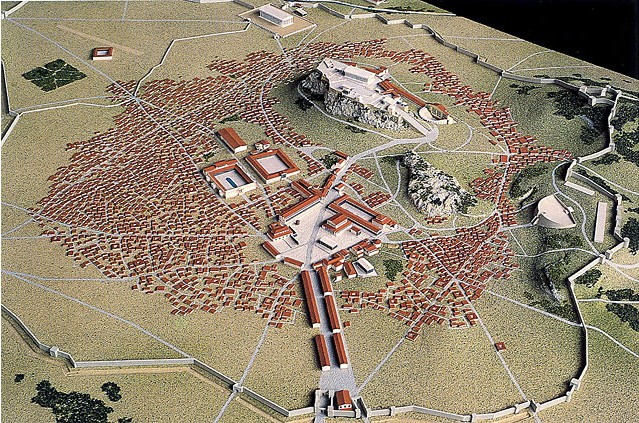
\includegraphics[width=7cm]{Preface/athens2ndc.jpg}
\caption{公元前2世纪雅典鸟瞰图}
%\label{default}
\end{center}
\end{figure}



\subsection{柏拉图的四元素说}

关于物质的理论,自古就有,比如古希腊的泰勒斯曾说“万物皆水”,后来又有人说万物是四种元素“水、气、土、火”构成。这就是所谓四元素说。

四元素说本来是古希腊人的常识(common sense),但柏拉图给这种关于物质的学说理论化,系统化了。这些内容被记载在柏拉图(427 BC — 347 BC)的宇宙论《蒂迈欧篇》中。

这里我们可以给出一个论证的概要:

\begin{itemize}
\item 

万物或者是可见的,或者是可以触摸的。可见是因为光,可以触摸是因为坚硬。光是火的性质,坚硬是土的性质,这样我们就有了“火和土”两种元素。

\item

万物是三维的,我们需要像“胶水”一样的元素把“火和土”按比例混合起来成为三维的物体。

这里柏拉图是通过构造如下数列来论证的:

\begin{equation*}
1=1^2=1^3, 2, 4=2^2, 8=2^3, 16=4^2, 32, 64=4^3,...
\end{equation*}

这里$1=1^3$,$8=2^3$,$64=4^3$,...,叫做立方数。

每两个立方数之间正好是两个数,比如1和8之间是2和4;而8和64之间是16和32。

柏拉图因此论证说需要两种元素在“火和土”之间调和使生成万物,这两种元素就是水和气。

\item

不论是可见,还是可以触摸,都可以归结为形状,而形状可以归结为多边形的拼合,多边形则可以归结为三角形的拼合。

三角形是研究形的基础,或说三角形是研究几何学的基础。

\item

柏拉图提出了两种基本的直角三角形:(1)等腰直角三角形,记做$T_{45}$;(2)一个锐角为$30^o$的直角三角形,记做$T_{30}$。

\item

利用两种基本的直角三角形可以拼成四种正多面体,即正四面体、正八面体、正六面体和正二十面体。

\begin{figure}[htbp]
\begin{center}
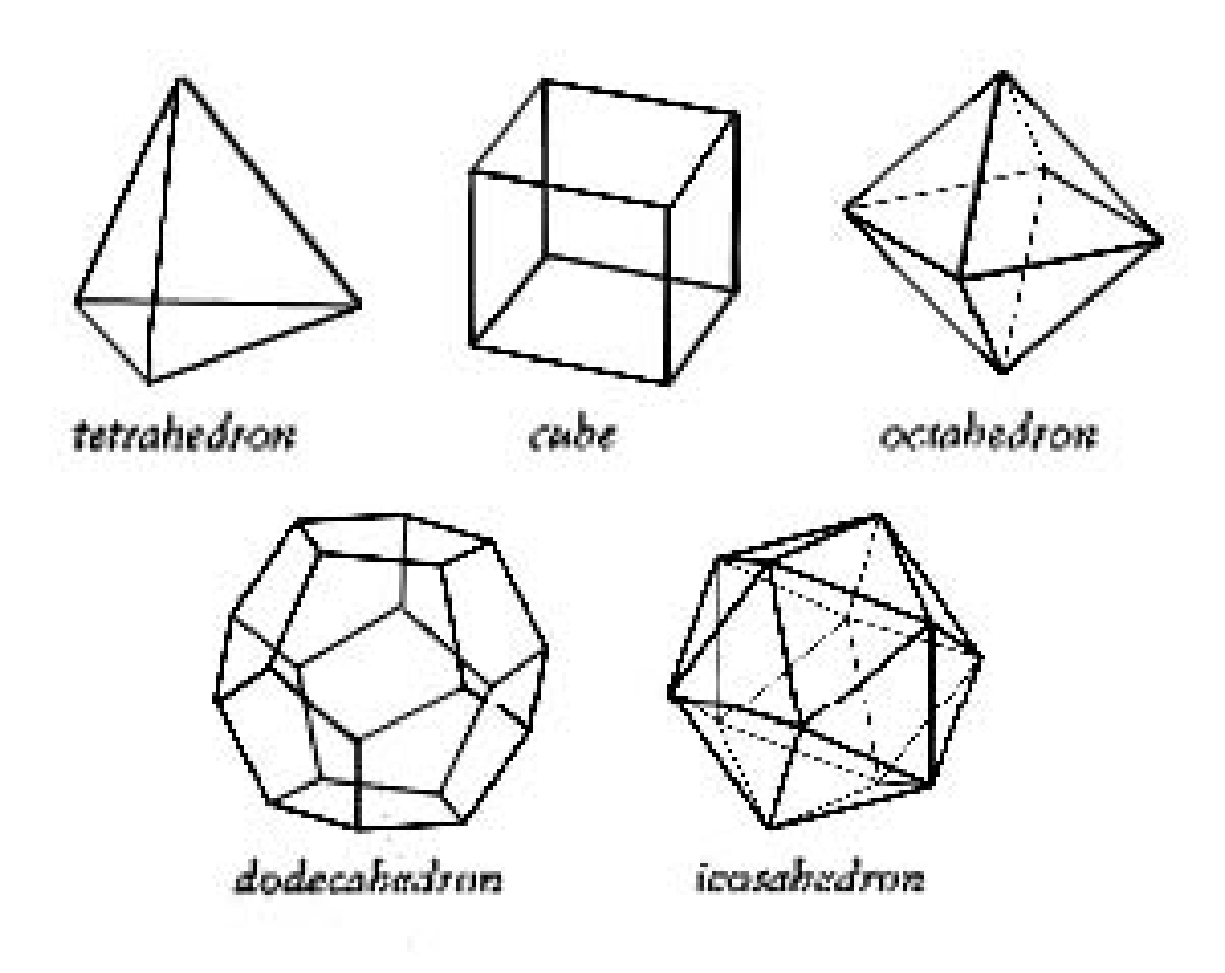
\includegraphics[width=10cm]{Preface/platonic-solids.ps}
\caption{五种正多面体,也称柏拉图多面体。这里面的正十二面体没有出现在对元素的构造中,这是柏拉图理论中欠缺美感的地方。}
%\label{default}
\end{center}
\end{figure}


\begin{enumerate}
\item 柏拉图认为立方体,即正六面体最稳定,因此把土的形定为正六面体。
\item 正四面体有最锐利的尖角,因此是最活跃的。火的形就是正四面体。
\item 剩下的还有气和水。因为气比水活跃,因此气的形就是正八面体。
\item 还剩下最后一个,正二十面体,是水的形。
\end{enumerate}

这些形都是很小的,用今天的话说就是“水气土火”的原子。并且这些原子还可以相互转化。

\begin{table}[htdp]
\caption{柏拉图的“元素说”}
\begin{center}
\begin{tabular}{|c|c|c|c|}
\hline
元素 & 正$n$面体 & 等腰直角三角形 & $30^o$直角三角形 \\
\hline
土 & 正六面体 & 12 & 0  \\
火 & 正四面体 & 0 & 8 \\
气 & 正八面体 & 0 & 16 \\
水 & 正二十面体 & 0 & 40\\
\hline
\end{tabular}
\end{center}
\label{default}
\end{table}%

\item

只有土是由等腰直角三角形围成的,因此土最稳定,它会被火溶解,可以被气或水分解,但不会转变成其它元素。

\item 

“火、气、水”都是由$30^o$的直角三角形围成的,因此可相互转换。比如,我们可以写出如下的反应方程式:

\begin{equation*}
1 Water \to 2 Gas + 1 Fire 
\end{equation*}

反应前有40个$T_{30}$,而反应后有$2 \times 16 + 8 = 40$个$T_{30}$。我们可以把上式与电解水的反应方程式比较:

\begin{equation*}
2 H_2 O \to 2 H_2 \uparrow + O_2 \uparrow
\end{equation*}

从思维的角度这是属于同一母型(Prototype)的。如果我们说古代思想会对近代科学有启迪作用,或我们说人总是在几种思维母型里打转转就毫不奇怪了。实际上量子力学的创建者,比如海森堡自幼就熟读《蒂迈欧篇》,如果说这些这些直观的图像会对他有潜移默化的影响可能并不夸张。

\end{itemize}

以上是柏拉图元素论的概要,当然这些都是非常粗糙的论证,而且经不起实验的定量检测,但元素之间可以互相转化,这个想法还是启迪了后来的炼金术,并最终导致了近代化学的出现。


\subsection{伊壁鸠鲁的原子论}

原子在古希腊语中不可再分的意思,这个不可再分固可以做物理上的拆分理解,亦可作逻辑上的不可再分(析)理解。比如刚才介绍的柏拉图关于“水气火土”四元素的理论就是逻辑上无法再分析的范例。

柏拉图的理论在古代是显学,2000多年来一直有稳定的传承,但它在古代并非没有对手,比如从德谟克利特、留基伯到伊壁鸠鲁、卢克莱修的原子论。但说实话这两种理论区别并不大,他们争执不休,以至于柏拉图都准备带弟子去焚烧德谟克利特的著作,并非是他们对自然真有什么本质的看法不同,毕竟都是一个时代对自然的看法。

关键的分歧是他们对伦理学和政治学的观点不一样,而古人的学问是个整体,伦理学的基础是哲学和科学,要驳倒对方,争取听众,釜底抽薪,攻击对方的科学观点是一个潜在的选择。

古代原子论者是今天所说的唯物论者,他们不相信灵魂,把生命看做是一堆原子具有功能性、活性或协调一致运动的集合。就好像是一把调谐良好的里拉琴,只要弦不断就能奏出美妙的音乐,对应于人的生命状态,而弦断则对应人亡,灵魂在这里是无所栖身的。没有灵魂,自然就没有死后世界,所有传统的道德说理就被架空了,Polis将处于危机之中。柏拉图派对唯物论者(或自然哲学家)的反感和敌对就在这里。

当然这并非我们现在的主题,我也不再继续展开讨论,而仅仅强调一点,即当我们讲到古代原子论的时候,我们应把柏拉图派的很多观点、理论也置于古代原子论的范畴内,而不仅仅是介绍自然哲学家的原子论。实际上很多柏拉图派的理念,比如天球的理念和近代原子模型是很接近的。对玻尔、海森堡这些哲学倾向很强的物理学家,很难想象他们没有阅读过《理想国》和《蒂迈欧篇》,而如果读过的话,他们一定对柏拉图的“数学-几何学”的宇宙模型印象深刻。

下面我将扼要地介绍伊壁鸠鲁的原子论,伊壁鸠鲁(341 BC — 270 BC)的《致希罗多德书信》是现存最早的关于原子论的记录,再早的比如德谟克利特和留基伯的就都已经失传了。

\begin{itemize}
\item 

在视觉上存在最小的点,再小我们就看不见了,这个视觉上的最小的点是有大小的。

由此类比:物质也是由最小的不可再分的最小单元构成的,再小是不存在的。

就这一点而言,伊壁鸠鲁的方案和柏拉图的方案是不同的,柏拉图的基础三角形没有明确地说存在最小、最基础的三角形。

今天的人大多会认为物质存在最小的不可再分的单元是很抽象的,或很难想象,但在古人那里也许未必。比如在中国古代是通过计量“肥而美”的“黑小米”来建立度量衡制度的,而在古代西方也有类似的比喻,比如卢克莱修在《物性论》中把水想象为大量罂粟籽的集合,比如阿基米德在《数沙者》中假想整个宇宙都充满了沙子,然后计算了整个宇宙中有多少粒沙子。

古人的数学观念是由“1,2,3,……”出发开始建立的,对他们来说想象一个由原子构成的世界其实是更简单的。这个原子就好比构成宇宙、万物的基础砖石,我们先寻求生命的结构和功能,进而问生命的可能的意义是什么?

\item

原子很小,因为我们谁也没见过原子。但我们没法假设原子的大小是绝对的0,因为如果那样的话,很多原子就无法构成万物了,而万物在我们的眼里是有体积的。

\item

原子如果有大小,那它就有部分,有形状。所以这里我们说的“不可再分”其实是物理意义下的,因为从几何学的角度,原子既然有部分,有形状,那它就可以在想象中继续分解。

这里区分了物理意义下的“分”,和数学意义下的“分”。前者对应今天的原子物理和量子力学,而后者对应的则是数学分析。

\item

原子既然有大小,有形状,它们之间就可以发生机械的相互作用,甚至结合成几个原子构成的具有特定功能的结构单元——分子。

没错,这都是伊壁鸠鲁天才的猜想。从字面上说已经很类似今天化学、甚至生物化学对结构和功能的解释。

当然,这里我们无需把这一天才的猜想神秘化,古代世界是个机械的世界,各种机械装置,从三列战舰、到攻城者德米特里乌斯的巨型攻城器械,古希腊人生活在这样一个机械无所不在的航海和贸易的时代,把原子想象成简单机械,把分子想象成具有特定功能的机械组合,进而把生命想象成极复杂的巨型机械都不是不可能的。

\end{itemize}

小结一下:柏拉图的四元素说和伊壁鸠鲁的原子论都是基于“形”的学说,但伊壁鸠鲁不能把他的理论数学化同时他的兴趣也不在于研究诸如——既然原子是有大小的,那么原子的大小到底是多少呢?——这类问题。

因此虽然古代原子论,无论是柏拉图的学说还是伊壁鸠鲁等自然哲学家的学说对人们想象原子有启发,但都不能说古希腊人已经接近了一个近代的原子论。近代原子论正如海森堡所说,是建立在一系列实验事实基础上的,当然还有概念体系和计算方法。

以下摘录海森堡在《物理学和哲学》第四章的一段讨论作为本小节的结束。

\begin{verbatim}
“在将原子物理学中的现代观点和希腊哲学作了类比之后,我们必须补充一个警告,即对这种类比不应有所误解。乍看起来,似乎希腊哲学家由于某种天才直觉而得到了与我们现代相同或很相似的结论,而我们的结论却是经过几个世纪的实验和数学方面的艰苦劳动才得到的。对我们的类比的这种解释无论如何是一种完全的误解。

在现代科学和希腊哲学之间有着巨大的差别,那就是现代科学的经验主义态度。自从伽利略和牛顿的时代以来,现代科学就已奠基于对自然的详细研究之上,奠基于这样一个假设之上,这就是:只有已被实验证实的或至少能被实验证实的陈述才是容许作出的。为了研究细节并在连续不断的变化中找到经久不变的定律,人们可用一个实验在自然中隔离出若干事件,这种观念希腊哲学家是没有想到过的。

由此可见,现代科学在一开始就立足于一个比古代哲学更谨慎同时也更巩固得多的基础之上。因此,现代物理学的陈述在某种意义上比希腊哲学更严肃得多。”
\end{verbatim}

\subsection{三角学}

\subsubsection{角度}

首先由圆出发,假设圆的半径是$R$,角$\theta$张成的圆弧是$l$。

\begin{figure}[htbp]
\begin{center}
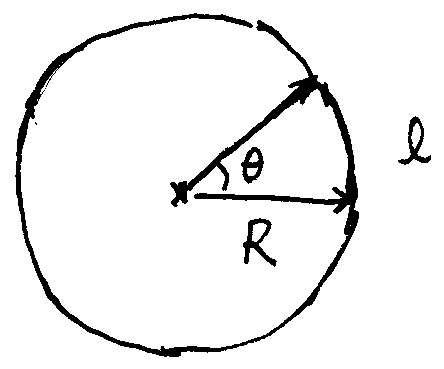
\includegraphics[width=4cm]{Preface/circle.png}
%\caption{default}
%\label{default}
\end{center}
\end{figure}

\begin{equation}
l = R \theta
\end{equation}

这其实构成了对角度$\theta$的定义,

\begin{equation}
\theta = \frac{l }{R }
\end{equation}

假想这个圆以半径$R$完整地转一圈,我们把这个角度定义为$2 \pi$,在平面上的张角只能取$0 \to 2 \pi$,$\pi$是个无理数,它近似地等于:

\begin{equation}
\pi = 3.14159265 ...
\end{equation}

这样定义的角度叫“弧度制”。但通常我们会把一个完整的圆周分成完全相等的360份,每一份称为一度,一度再等分为60份,每份叫一分,一分再等分为60份,每份叫1秒,这就是所谓“度分秒”制。

“度分秒制”的好处是,60很容易被2、3、4、5、6等分,这对古人精确地计算星星在天空中的方位是很重要的。比如:17度25分30秒可记为:

\begin{equation*}
17^o 25' 30''
\end{equation*}

我们可以把一个圆周对应的张角分成完全相等的四份,每一份都是个直角,一个直角在弧度制下是$\frac{\pi}{4}$,而在度分秒制下则是$90^o$。

\subsubsection{正弦和余弦函数}

现在来考虑一个直角三角形,即一个角是直角的三角形:

\begin{figure}[htbp]
\begin{center}
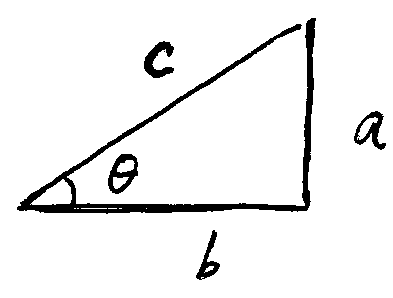
\includegraphics[width=4cm]{Preface/rectriangle.png}
%\caption{default}
%\label{default}
\end{center}
\end{figure}

假设其中一个锐角是$\theta$,$\theta$所对的直角边是$a$,另一条直角边是$b$,斜边是$c$,我们有毕达哥拉斯定理:“斜边的平方等于两直角边的平方和”。

\begin{equation}
c^2 = a^2 + b^2
\end{equation}

我们可定义正弦和余弦函数如下:

\begin{eqnarray}
\sin \theta & = & \frac{a}{c} \\
\cos \theta & = & \frac{b}{c}
\end{eqnarray}

即正弦函数被定义为对边$a$与斜边$c$之比,而余弦函数被定义为邻边$b$和斜边$c$之比。

\begin{figure}[htbp]
\begin{center}
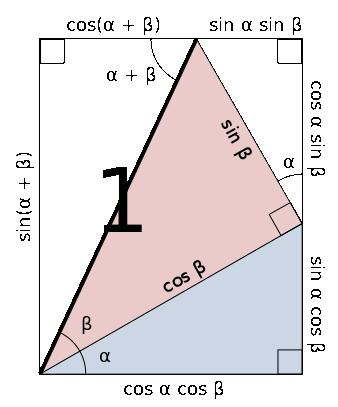
\includegraphics[width=6.5cm]{Preface/angleaddition.png}
\caption{两个角度相加的正弦和余弦:$\sin (\alpha + \beta) = \sin \alpha \cos \beta + \cos \alpha \sin \beta$, $\cos (\alpha + \beta ) = \cos \alpha \cos \beta - \sin \alpha \sin \beta$}
%\label{default}
\end{center}
\end{figure}

类似地我们还可定义正切函数($\tan \theta$)和余切函数($\cot \theta$):

\begin{eqnarray}
\tan \theta & = & \frac{a}{b} \\
\cot \theta & = & \frac{b}{a}
\end{eqnarray}

现在考虑一个单位圆,即半径为1的圆,假设圆上一点逆时针地围绕圆心转动起来。这一点向$x$轴的投影是$x$,向$y$轴的投影是$y$。



\begin{figure}[htbp]
\begin{center}
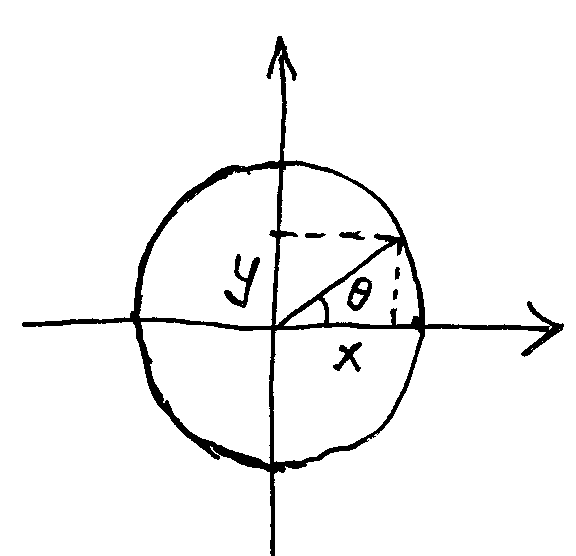
\includegraphics[width=4cm]{Preface/circlexy.png}
%\caption{default}
%\label{default}
\end{center}
\end{figure}


\begin{eqnarray*}
x & = & \cos \theta \\
y & = &  \sin \theta 
\end{eqnarray*}

据说第一个三角函数表(Trigonometric table)是古希腊天文学家伊巴古(又译作喜帕恰斯,190-125 BC)编纂的。

\begin{table}[htdp]
\caption{常见三角函数的取值}
\begin{center}
\begin{tabular}{|c|c|c|}
\hline
$\theta$ & $\sin \theta$ &  $\cos \theta$ \\
\hline
0  &  0 &  1 \\
$\pi/4$ & $\frac{1}{\sqrt 2}$  & $\frac{1}{\sqrt 2}$ \\
$\pi/2$ & 1  &  0 \\
$\pi$ & 0 & -1 \\
\hline
\end{tabular}
\end{center}
%\label{default}
\end{table}%

根据上表,我们可以计算:

\begin{eqnarray*}
\sin ( \theta + \pi /2) & = & \sin \theta \cos \pi /2 + \cos \theta  \sin \pi/2 = \cos \theta \\
\cos ( \theta + \pi /2) & = & \cos  \theta \cos \pi /2 - \sin \theta \sin \pi/2 = - \sin \theta
\end{eqnarray*}

于是得到正弦/余弦函数的性质:

\begin{eqnarray}
\sin ( \theta + \pi /2 ) & = & \cos \theta \\
\cos ( \theta + \pi /2) & = & - \sin \theta
\end{eqnarray}



当$\theta$从$0 \to 2\pi$变化时,$x$的取值将从$1 \to 0 \to -1 \to 0 \to 1$,然后重复,而$y$的取值将从$0 \to 1 \to 0 \to -1 \to 0$,然后重复。

\begin{figure}[htbp]
\begin{center}
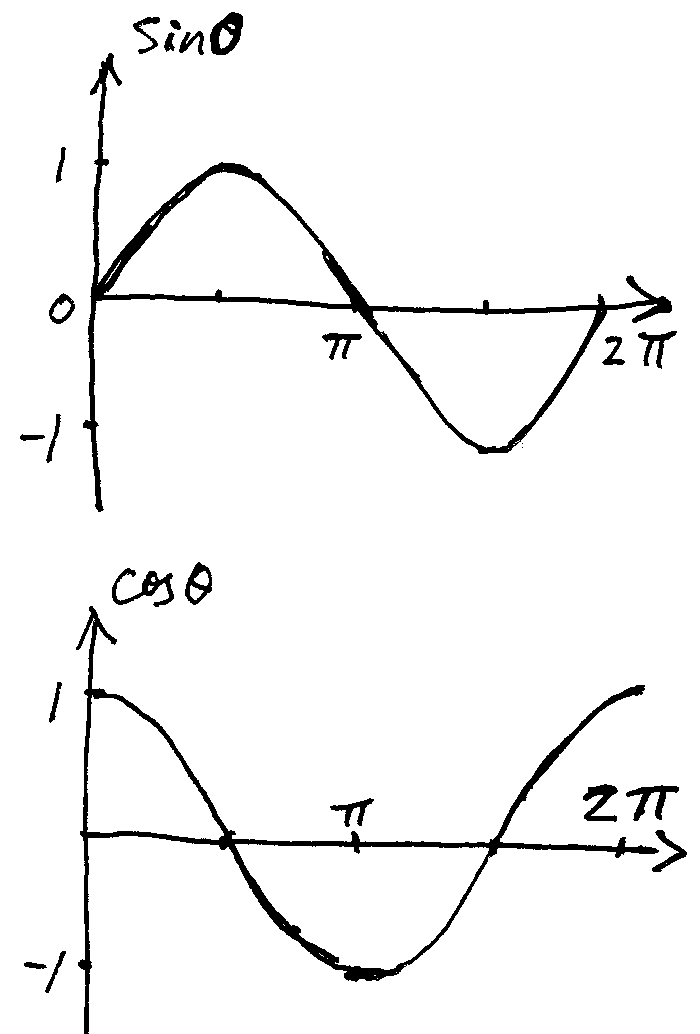
\includegraphics[width=4cm]{Preface/sincostheta.png}
%\caption{default}
%\label{default}
\end{center}
\end{figure}

这种周期性的运动很类似月相的变化,望是满月,朔是新月,由于月球围绕地球的运动,我们在地球上观察将看到月亮由月初的新月,到月中(十五)的满月,然后到月末又回到新月,然后重复。

在此意义下我们称$\theta$为相位(phase)。

正弦和余弦函数在物理学中的用处很多,比如它是弹簧振子的解,是波动方程的解等。

\subsubsection{振动}

对振动而言,相位是:

\begin{equation}
\theta = \omega t 
\end{equation}

这里$\omega$叫角频率,当$\omega t = 2 \pi$时,振动正好重复一个周期$T$,

\begin{equation}
T = \frac{2 \pi}{\omega}
\end{equation}

描述振动的方程是:

\begin{equation}
A \cos \omega t
\end{equation}

$A$叫做振幅,振动将在$A \to 0 \to -A \to 0 \to A$重复发生。

\begin{table}[htdp]
\caption{$A \cos \omega t$ 描述的运动}
\begin{center}
\begin{tabular}{|c|c|c|}
\hline
时间 & 相位 &  位置 \\
\hline
0 & 0 & A \\
T/4 & $\pi /2 $ & 0 \\
T/2 & $\pi$ & -A \\
3T/4 & $3 \pi /2  $ &  0 \\
T &  $2\pi$  & A \\
\hline
\end{tabular}
\end{center}
%\label{default}
\end{table}%

但有时候当$t = 0$时,我们就已经有了一个非零的相位$\theta_0$了,这时描述振动的方程将变成:

\begin{equation}
A \cos (\omega t + \theta_0)
\end{equation}

这里$\theta_0$叫做初相位(initial phase),我们管用正弦/余弦函数描述的振动叫简谐振动。

\subsubsection{波动}

振动是在时间变量上的重复。波动是在时间和空间上的重复。我们所处的世界是一维的时间再加上三维的空间。为了简单,我们先考虑空间也是一维的情况。

假设我们在体育场里造人浪(Mexican wave),开始的时候也许只有一个人重复地做“站起-欢呼-坐下”,再“站起-欢呼”再“坐下”,然后重复的动作,他旁边紧挨着的人注意到他的动作,也会跟着模仿他的动作,但因为距离的存在,旁边的人要反应过来跟着他一起做需要过一段时间,即有个时间的延迟。

\begin{figure}[htbp]
\begin{center}
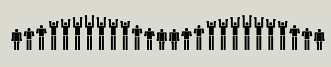
\includegraphics[width=6cm]{Preface/mexicanwave.png}
\caption{墨西哥人浪起源于1986年的墨西哥世界杯。在那届世界杯上,热情的球迷自发地运用一种交替起立欢呼的方式自娱自乐,为球队加油,从远处看就像一阵阵的海浪。}
%\label{default}
\end{center}
\end{figure}


假设人与人之间的间距是$\Delta x$,时间的延迟是$\Delta t$,波动在空间上传播的速度就是:

\begin{equation}
v = \frac{\Delta x }{\Delta t}
\end{equation}

假设第一个人正好完成了一个振动的周期$T$:

\begin{verbatim}
    “坐着、站起、欢呼、坐下、坐着”
\end{verbatim}

这时如果他抬头看的话,他会发现距离他$\lambda$远处某个人正处于和他一样“坐着”的状态,而且他马上就要站起来了,因为他紧邻的人已经在做“站起”的动作了。

可以设想,这两个相距$\lambda$的人将做完全同步的振动,在我们外人看来,他们一起“坐着”,又一起“站起”,一起“欢呼”,……

如果用振动的语言说的话,它们的相位是相同的。但这么说让我们不舒服,因为毕竟后一个人的运动要晚于第一个人,我们说,

\begin{center}
“空间相距$\lambda$远的两个点,它们运动的相位正好差$2 \pi$”
\end{center}

这样说就舒服了。

现在我们假设体育场里已经造起了人浪,我们应该如何描述它呢?这是一个以空间位置$x$和时间$t$为变量的函数。

假设$t$固定,比如令$t = 0$我们得到一个随$x$起伏变化的函数,这就相当于是照相机照的快照,在某个时间运动冻结了,但仍会在空间$x$上有个分布,假设这个函数是:

\begin{equation*}
\psi (x, t = 0) 
\end{equation*}

这个分布其实就是个波形,它围绕$x = 0$附近展开。单独看这个随$x$起伏的波形,它也是周期性的,是空间调制意义下的周期性,每增加波长$\lambda$,$\psi$就重复。

假设$\psi$可以表示为一个正弦/余弦函数,这意味着:$x$每增加$\lambda$,相位的变化是$2 \pi$。即:

\begin{equation*}
\psi (x, t = 0) = A \cos \frac{2 \pi x}{ \lambda}
\end{equation*}

\begin{figure}[htbp]
\begin{center}
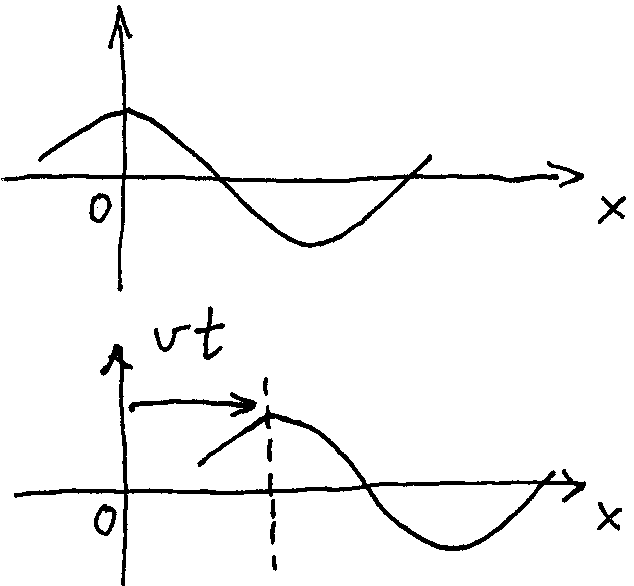
\includegraphics[width=6cm]{Preface/waveaftervt.png}
\caption{经过时间$t$,波形会向前移动$vt$,或者说是函数沿$x$方向发生了平移,平移前函数是$\psi(x)$,而平移后函数是$\psi(x - vt)$。}
%\label{default}
\end{center}
\end{figure}



现在假设时间是$t$,并且$t > 0$,波形会向前传播,时间$t$波形向前移动了$vt$,这意味着波函数是在$x = vt$附近展开的。

\begin{equation*}
\psi(x,t) = A \cos \frac{2 \pi}{\lambda} \left( x - vt \right)
\end{equation*}

假设波形移动$\lambda$需要花费时间$T$,波形移动的速度$v$是:

\begin{equation*}
v = \frac{\lambda}{ T }
\end{equation*}

波函数$\psi(x,t)$变成:

\begin{equation}
\psi(x, t) = A \cos   2\pi \left(  \frac{x}{\lambda} - \frac{t}{T}   \right)
\end{equation}

定义波矢$k$,和角频率$\omega$分别为:

\begin{eqnarray}
k &=& \frac{2 \pi}{\lambda} \\
\omega &=& \frac{2 \pi}{T}
\end{eqnarray}

波函数取常见的形式:

\begin{equation}
\psi (x,t )= A \cos \left( k x - \omega t \right)
\end{equation}

现在相位是:

\begin{equation*}
k x - \omega t
\end{equation*}

固定时间,我们会得到波动随空间的分布,$x$越大,相位也越大。固定位置,我们会得到波动就在这个位置随时间的振动。



%%%%%%%


%%%%%%%

\subsection*{练习}

\begin{enumerate}
\item 

假设人眼瞳孔大小是2mm,可见光波长是550nm,利用公式:

\begin{equation*}
\theta = 1.22 \cdot \frac{\lambda}{D}
\end{equation*}

估算人眼的角分辨本领,并把结果换算为“度分秒”为单位。

据说第谷(1546 — 1601)对星星观察的准确度能够达到二弧分,已经逼近肉眼的理论极限,当然夜晚观星瞳孔会放大,这有利于提高他的精度。

\end{enumerate}

\newpage

\section{运动的观念}

运动是个让人讨厌的概念,这意味着运动着的物体它即在这里,它又不在这里,我们该如何描述它呢?在我们的日常经验里,运动得足够快的物体,我们是“看不见”的,也“捉不住”,因为物体运动的太快,我们的眼睛还没来得及对它们成像,它们就已经跑掉了。

我们从来没有看见过运动的物体,我们看到的都是静态图像,在某个时刻$t_0$开始,持续了某个特征时间$\Delta t$,在这段特征时间里,物体基本不动,比如物体位置的变化小于人眼的视觉分辨极限,于是我们得到了一幅完全静态的图像。每个物体的边界和位置在我们的眼睛里都有很好的定义。

这是一个很夸张的讨论,并且因为这个讨论涉及视觉的生理问题而,压根就是错误的。人眼(+大脑皮层)不仅仅是接收光信号的器官,同时它还在主动地对光信号进行处理,真实的视觉是人眼(+大脑皮层)主动参与的结果。

但以上讨论还是有益的,比如在生活中有时我们会看不清,不论是看“静”物,还是看“动”物,我们都有可能看不清,不但看不清,我们还特想看清,这时候我们一般会眯起眼睛,使劲盯着自己想看清的东西使劲看,这就是所谓凝视(gaze)。

凝视就是暂时中止人眼(+大脑皮层)主动处理视觉信息,迫使人眼(+大脑皮层)清空成见和既有的算法,完全被动地接受物体发出的光信号,这就是把人眼纯粹当照相机镜头用了。

实际上再怎么盯着看,我们也看不清飞奔骏马的步态或子弹穿透苹果的细节,但人就是对视觉的东西有好奇,越是看不清,就越想盯着看,于是高速照相机取代了我们的眼睛。得到了完全“客观”的图像,这里可完全没有人眼(+大脑皮层)主观的参与。

\begin{figure}[htbp]
\begin{center}
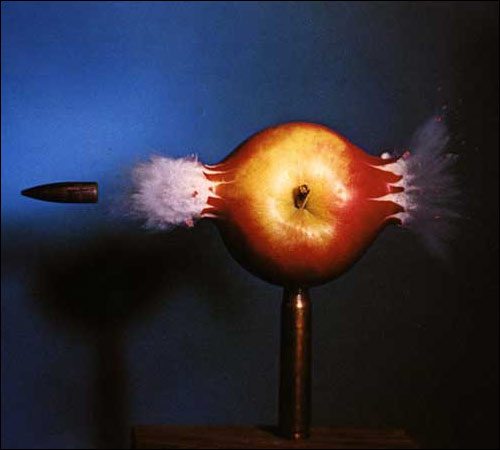
\includegraphics[width=5cm]{Preface/shootapple.jpg}
%\caption{default}
%\label{default}
\end{center}
\end{figure}

人面对运动最终会求助凝视或高速摄像机,说明人是通过“静止”去认识“运动”的,或人压根对“静止”的图像就有偏好,而本能地讨厌“运动”和“变化”,特别是那些无法预知未来的“运动”和“变化”。

\subsection{人对静止图像的偏好}

下面我将举几个例子来说明人对静止图像的偏好,所谓“静止”就是不变化了,我们可以用等式,比例关系等来描述物理规律,而不是用微分方程。

\begin{enumerate}
\item 

阿基米德的杠杆定律:

杠杆定律不讨论杆不平的状况,当杆平的时候,左右两臂的臂长和施加在两臂的力满足以下关系:

\begin{equation}
W_L R_L  = W_R R_R 
\end{equation}

我们可以设想杠杆稍微动起来,比如逆时针转动了$\theta$角度,假设$\theta$很小。

左臂会向下转,角度$\theta$张成的圆弧长度为:

\begin{equation*}
R_L \theta
\end{equation*}

即左侧重物$W_L$会向下移动$R_L \theta$。

重力方向向下,即重物$W_L$移动的方向和重力的方向一致。我们在簿记表中记做“+”,即$W_L$做正功。

\begin{equation*}
W_L  R_L \theta
\end{equation*}

类似地右臂会向上转,角度$\theta$张成的圆弧长度为:

\begin{equation*}
R_R \theta
\end{equation*}

即右侧重物$W_R$会向上移动$R_R \theta $。

重力方向向下,即重物$W_R$移动的方向和重力的方向相反。我们在簿记表中记做“-”,即$W_R$做负功。

\begin{equation*}
W_R R_R \theta
\end{equation*}

根据杠杆定律$W_L R_L  = W_R R_R$,簿记表中的正负贡献正好相抵。

杠杆定律关注的是达到平衡/静止状态的条件。

\item

阿基米德的浮力定律:

物体浸泡在液体中的浮力等于它排开液体的重量。

用今天的物理概念很容易证明。假设一个规则的物体,比如立方体放入水中,或者它比水轻,或者它比水重。

如果它比水轻的话,假设立方体浸入水的深度为$h$,水中压强是各个方向都一样的,并且和深度有关,满足关系:

\begin{equation}
P = \rho_0 g h
\end{equation}

这个压强作用于立方体的底部,方向向上,大小是:

\begin{equation*}
PS = \rho_0 g h S = \rho_0 V g = M_0 g
\end{equation*}

这里$h S$就是排开水的体积,$M_0 g $就是排开水的重量。

假设立方体比水重的证明与之类似,立方体会全部浸入水中,假设上表面距离水面$h$,下表面距离水面为$h + L$。

浮力就是上下表面的压力差,因为作用于下表面的压力较大,所以浮力的方向是向上的。

\begin{equation*}
F = \rho_0 g (h + L) S - \rho_0 g h S = \rho_0 g L S = \rho_0 V g
\end{equation*}

这里$V = LS$是立方体的体积,浮力的大小仍是排开水的重量$\rho_0 V g$。

\item

亚里士多德对运动快慢的讨论:

亚里士多德说重物下落速度较快,轻物下落速度较慢。但亚里士多德讨论的是匀速运动的物体,他其实也注意到物体在刚刚落下的时候运动速度是在变化的,但他拒绝讨论这一阶段,或者说他当时尚不具备讨论速度变化的数学手段。

当重物下落时,由于下落速度$v$的存在,重物会受到一个向上的粘滞阻力。根据斯托克斯定律:粘滞阻力的大小正比于下落速度$v$,此外粘滞阻力也正比于重物的大小,如果是球的话,就正比于球的半径$r$,写成数学式子:

\begin{equation}
F = 6 \pi \eta r v
\end{equation}

这里$\eta$是粘滞系数,和介质及重物的材质有关。实际上空气的粘滞系数比较小,所以重物要下落比较长的距离才会积累到足够大的速度以与重力抵消。为了演示粘滞阻力可以很快抵消掉重力,我们一般都是在粘稠的油中做这个实验,用不同的油,不同直径,不同密度的球来做这个实验。

球的重量可表示为:

\begin{equation*}
Mg = \rho V g = \rho \frac{4 \pi r^3}{3} g
\end{equation*}

考虑到球本身还有浮力$F'$,这个浮力和球排开的流体的重量正好相等。

\begin{equation*}
F' = \rho_0 V g = \rho_0 \frac{4 \pi r^3}{3} g
\end{equation*}

向上的力是浮力$F'$加上粘滞阻力$F$,向下的力是重量$Mg$,我们得到平衡条件:

\begin{equation*}
\rho_0 V g + 6 \pi \eta r v = \rho V g
\end{equation*}

即:

\begin{equation}
( \rho - \rho_0  ) V g = 6 \pi \eta r v
\end{equation}

如果是空气的话,铁球的密度远大于空气的密度,$(\rho - \rho_0) V g = Mg $,就是铁球的重量。球最终匀速落下的速度:

\begin{equation}
v = \frac{Mg}{ 6 \pi \eta r  }
\end{equation}

即物体越重落下的越快。这就是亚里士多德的结论。

必须声明以上讨论是基于现代物理语言和符号的,但这确实是亚里士多德的思路。

\item

最后一个例子是行星运动:

行星运动的轨迹可以是正圆,可以是椭圆,也可以是抛物线,甚至是双曲线(后两种其实已经不是行星了,因为它们注定会飞行到距离恒星无穷远的地方)。

这其实是很复杂的,除正圆的运动外,即行星围绕恒星做正圆的运动是匀速运动,剩下的都不是匀速运动。

我们其实是通过轨迹来理解行星的运动的,不论是椭圆还是双曲线对我们来说都是静态的图形,运动在这里被我们取消了。

当然我们可以指着行星运动的轨迹说,行星离恒星越近它们的速度就越大等等。

比如对椭圆轨道而言,在近日点的速度$v_n$,和在近日点时行星距离恒星的距离$R_n$,与远日点的速度$v_f$,和在远日点时行星距离恒星的距离$R_f$满足:

\begin{equation*}
v_n R_n = v_f R_f
\end{equation*}

\end{enumerate}

\subsection{伽利略的斜面实验}

要想定量地研究运动,必须能对时间进行精确的测定。亚里士多德之所以只研究匀速的运动和他缺乏精确地测量时间的手段有关。

传说,伽利略(1564 — 1642)为了反驳亚里士多德的落体理论,曾登上55米高的比萨斜塔做了著名的落体实验。但这听上去更像是个表演,类似马戏团的表演,因为它仍然缺乏测量和数据的支撑。

我们可以估算一下落体从55米高落下需要多少时间。

\begin{equation}
s = \frac{1}{2} g t^2
\end{equation}

这里$g = 9.8 m/s^2$是地球表面的重力加速度。解出:

\begin{equation*}
t = \sqrt{\frac{2 s}{ g}} = 3.35(s)
\end{equation*}

即大约只需要3秒,要精确地测量这个时间在伽利略的时代是很困难的。这就需要发挥高超的实验技艺将问题转化。

伽利略到底有没有到比萨斜塔去作秀我们不知道,但伽利略确实做过一个“斜面落体实验”。

\begin{itemize}
\item 

首先取来一个长约7米的木板,在木板上刻一条一指宽的槽,槽要非常直而且平滑。

\item

把木板倾斜放置,让一个坚硬、光滑的黄铜球沿木板上的槽滚落。

让铜球沿倾斜放置的木板滚下来是可以有效地减小加速运动的加速度的。这当然会减轻精确测量时间的压力。

\item

在伽利略的时代最精确的测量时间的装置是水钟。

水钟有巨大的装水容器,水会从容器底部的细管流出,由于装水容器的横截面积很大,我们可以忽略水面高度的变化,只要细管的管口经过精细的打磨和加工,经细管流出水的速度就是恒定的。

水钟可以非常精确地计时,这是伽利略斜面实验得以完成的前提。

\item

让铜球从斜面上滚落,开始滚动的瞬间我们打开水钟,当球运动到特定的位置,比如:10厘米,20厘米,30厘米,……我们关掉水钟。

我们把水钟里流出的水收集起来,然后通过非常精密的天平(杠杆原理)去测量它们的质量,水的质量是正比于——铜球滚落特定距离——所用时间的。

\end{itemize}

其实水钟也是希腊-罗马时代的发明,原则上说古典时代人们也是可以做伽利略的“斜面实验”的。

对此我的评论是:(1)首先我们需膜拜伽利略构思实验之精妙;(2)其次即便某位哲学家在2000多年前就做过“斜面实验”,但他也不会有效地撬动当时主流的思想,因为孤立的一个实验(或理论)并没有多少意义,必须把它放入一个潮流里,它的意义才会显现出来。(3)伽利略的这项工作是近代物理学一系列工作最开始的几个之一。评价一项实验,一个工作,重要的是看它引发了什么。

在伽利略的手稿中,我们发现了这么一个表格:

\begin{table}[htdp]
\caption{伽利略的斜面实验记录}
\begin{center}
\begin{tabular}{|c|c|c|}
\hline
$t^2$ & t & s \\
\hline
1 & 1 & 32 \\
4 & 2 & 130+ \\
9 & 3 & 298+ \\
16 & 4 & 526+ \\
25 & 5 & 824 \\
36 & 6 & 1192 \\
49 & 7 & 1600 \\
64 & 8 & 2104 \\
\hline
\end{tabular}
\end{center}
\label{default}
\end{table}%

表格中第三列是距离,单位不是很清楚,但想必是在他7米长的大斜面上做的。第二列是时间,这个时间倒不一定是用水钟测量的,因为它是1、2、3……罗列的,很有可能是人的脉搏或单摆。

第一列数字是后加上去的,因为笔迹的颜色不一样,看来伽利略猜测到这里面的规律了,即铜球延斜面滚落的距离$s$正比于所需时间$t$的平方。

\begin{equation}
s \propto t^2
\end{equation}

可以想象当伽利略达到这个猜测后,他就可以利用水钟做更精确的实验以验证这一结果。比如他可以让铜球延斜面滚落:10厘米,40厘米,90厘米,160厘米,……以验证它们对应的滚落时间是否接近于:$1: 2^2: 3^2 : 4^2 : ...$

\subsection{微分}

用现代的语言,伽利略发现的规律是,

\begin{equation}
s(t) = \frac{1}{2} a t^2
\end{equation}

即加速度恒定条件下,物体的运动。

对这种运动速度是时时刻刻变化的。此时再把速度$v$定义成距离和时间之比就不合适了。

\begin{equation}
v = \frac{s}{t}
\end{equation}

由伽利略测出的数据,我们有一种直觉,即运动速度是越来越快的。我们现在用对距离的微分来定义速度:

\begin{equation}
v = \frac{d s}{d t } = \lim\limits_{\Delta t \to 0} \frac{s(t + \Delta t) - s(t)}{\Delta t}
\end{equation}

这里的$\lim\limits_{\Delta t \to 0}$表示一个取极限的过程,即构造一个序列:$\Delta t = 1 s, 0.1 s, 0.001s , ...$用越来越小的时间间隔去反复计算$\frac{s(t + \Delta t) - s(t)}{\Delta t}$,看什么时候商的取值会稳定下来。这个其实就是做工程的思路,关注结果,不关心形式是否优美。

或者我们把分子展开:

\begin{equation*}
s(t + \Delta t) - s(t) = \frac{a}{2} \left( t^2 + 2t \Delta t + (\Delta t)^2 - t^2 \right)
\end{equation*}

考虑到$ \Delta t \to 0 $是个很小很小的数,那么$( \Delta t )^2$是个更小更小的数,我们管$(\Delta t) ^2$叫高阶无穷小,在有低阶无穷小项$2 t \Delta t$存在的情况下,我们可以放心地忽略$( \Delta t )^2$。


现在公式变成了:

\begin{equation*}
v(t) = \frac{a}{2}  \cdot  \frac{2t \Delta t}{\Delta t } = at
\end{equation*}

现在速度确实变成一个和时间$t$有关的函数。即速度在时时刻刻地变化着。

以下罗列求微分运算的主要结果:

\begin{enumerate}
\item 

对幂函数$x^n$求微分,假设这里$n > 0$,并且是整数。

求微分也叫求导,记做$(x^n)'$

\begin{equation}
( x^n )' = \lim\limits_{\eta \to 0} \frac{(x+ \eta)^n - x^n}{\eta}
\end{equation}

这里需要计算$(x + \eta)^n$

\begin{eqnarray*}
( x + \eta)^n & = & (x + \eta)(x + \eta) ... (x + \eta)   \\
{} & = & x^n + n x^{n-1} \eta + \frac{n(n-1)}{2} x^{n-2} \eta^2 + ... + \eta^n
\end{eqnarray*}

这里涉及$n$个$( x + \eta)$连乘,

\begin{itemize}
\item 

第一项自然是$x^n$;

\item

第二项是一阶无穷小,即包含$\eta$的项,这意味着要从$n$个$( x + \eta)$中挑出一个$\eta$来,这有$n$种可能性;

\item

接下来的一项,是包含$\eta^2$的项,这意味着要从$n$个$( x + \eta)$挑出两个$\eta$来,但这个挑选和次序无关,因此有$\frac{n (n -1)}{2}$。

即第一次挑选有$n$种可能性,第二次挑选只能从剩下的$n-1$项里选,因此有$n-1$种可能性,$n(n-1)$是考虑挑选次序的,即认为先选第一项再选第二项,和先选第二项再选第一项是两种情形,但在我们这里与次序无关,因此需要再除以2。

\item

一般地,包含$\eta^m$的项,其系数是$\frac{n(n-1)...(n-m+1)}{m!}$

这里$m!$被定义为:

\begin{equation}
m! = m (m-1) (m-2) ... 3 \cdot 2 \cdot 1
\end{equation}

即$m$个不同的人排队,从左排到右的所有方式数,先是从$m$个人里随便挑一个出来,排第一个儿,有$m$种可能性,然后在剩下的$(m-1)$个人挑一个出来排第二个儿,有$m-1$种可能性……


\item

最后一项,包含$\eta^n$的项,其系数是$\frac{n!}{n!} = 1$

\end{itemize}

现在我们可计算出$x^n$的导数是:

\begin{equation}
(x^n)' = \lim\limits_{\eta \to 0} \frac{n x^{n-1} \eta}{\eta } = n x^{n-1} 
\end{equation}

\item

我们定义一个新的函数$e^x$

\begin{equation}
e^x = \sum\limits_{n=0}^{\infty} \frac{x^n}{n!} = 1+x + \frac{x^2}{2} + ...
\end{equation}

可以证明$e^x$的导数还是它自己。

\begin{eqnarray*}
(e^x)' & = & ( 1 + x + \frac{x^2}{2} +  \frac{x^3}{3!} +... + \frac{x^n}{n!}  +... )' \\
{} & = & 1 + x + \frac{x^2}{2} + ... + \frac{x^{n-1}}{(n-1)!} + ...
\end{eqnarray*}

那么$e$等于多少呢?

我们取$x =1$,会得到一个估算$e$的数列求和:

\begin{equation}
e = 1 + 1 + \frac{1}{2!} + \frac{1}{3!} + ... + \frac{1}{n!} + ...
\end{equation}

我们管$e$叫做自然指数,也叫欧拉数(Euler's Number),它大约是:

\begin{equation}
e \approx 2.71828
\end{equation}

很重要地,$e^x$的导数还是$e^x$

\begin{equation}
(e^x)' = \frac{d}{dx} e^x = e^x
\end{equation}

\item

假设$f(x)$和$g(x)$是两个函数,存在微分$\frac{df}{dx}$,$\frac{dg}{dx}$,对函数$f(g)$求微分:

\begin{equation}
\frac{d f(g)}{d x} = \frac{d f}{d g} \frac{d g}{ d x}
\end{equation}

作为一个简单的例子,对$f(ax)$求微分:

\begin{equation}
\frac{d f(ax)}{d x} = a \frac{d f(x)}{ d x} 
\end{equation}

\item

假设$f(x) = u(x) v(x)$,导数$u'$, $v'$都存在,求$f'$

\begin{eqnarray*}
f' & = & \lim\limits_{\eta \to 0} \frac{ u(x+\eta) v (x+ \eta) - u(x) v(x) }{ \eta } \\
{} & = & \frac{  u(x+\eta) v (x+ \eta) - u(x+\eta) v + u(x+\eta) v - u v  }{\eta} \\
{} & = & u'v + u v'
\end{eqnarray*}

即:

\begin{equation}
( u v)' = u' v + u v'
\end{equation}

\item

函数$y = f(x)$是由$x \to y$的映射$f$,我们也可定义逆映射$f^{-1}: y \to x$,记做:$x = f^{-1}(y)$。

假设存在导数$f'$,逆函数$(f^{-1})'$的导数如何表示?

\begin{equation*}
\left(  f^{-1} (y) \right)' = \frac{dx}{dy} = \frac{1}{dy/dx} = \frac{1}{ f'(x) }
\end{equation*}

但我们现在必须把右侧的变量$x$变为以$y$为变量,即需代入:$x = f^{-1} (y)$

\begin{equation*}
\left(  f^{-1} (y) \right)' = \frac{1}{ f'( f^{-1} (y)) }
\end{equation*}

然后我们再把等式左侧和右侧的变量都改变为$x$,

\begin{equation}
\left(  f^{-1} (x) \right)' = \frac{1}{ f'( f^{-1} (x)) }
\end{equation}

作为一个例子,我们来研究一下$e^x$的逆函数:

\begin{eqnarray*}
y &=& e^x \\
x &=& \ln y
\end{eqnarray*}

即:

\begin{eqnarray*}
\ln e^x & = & x \\
e^{\ln y} & = & y
\end{eqnarray*}

现在来计算$(\ln y )'$

\begin{equation*}
( \ln y)' = \frac{1}{dy/dx} = \frac{1}{e^x} = \frac{1}{e^{\ln y}} = \frac{1}{y} 
\end{equation*}

最后我们把$y$换成$x$,

\begin{equation}
( \ln x)' = \frac{1}{x}
\end{equation}

\item

考虑函数$f(x) = \frac{u(x)}{v(x)}$,假设导数$u'$, $v'$存在,求导数$f'$。

根据微分/导数的定义:

\begin{equation*}
f' = \lim\limits_{\eta \to 0} \frac{1}{\eta} \left( \frac{u(x+\eta)}{v(x+\eta)} - \frac{u}{v} \right)
\end{equation*}

其中:

\begin{equation*}
\frac{u(x+\eta)}{v(x+\eta)} - \frac{u}{v} = \frac{ u(x+\eta) v - u v(x+\eta)  }{ v(x+\eta) v }
\end{equation*}

其中:

\begin{eqnarray*}
u(x+\eta) v - u v(x+\eta) & = & u(x+\eta) v - uv + u v - u v(x+\eta) \\
{} & = & (u(x+\eta)-u)v - u(v(x+\eta)-v )
\end{eqnarray*}

因此:

\begin{equation}
\left( \frac{u}{v} \right)' = \frac{ u' v - u v' }{v^2}
\end{equation}

现举一例:

比如我们计算$\frac{1}{x}$的导数$\left( \frac{1}{x} \right)'$

\begin{equation*}
\left( \frac{1}{x} \right)' = \frac{ - 1 }{x^2} = -x^{-2}
\end{equation*}

类似地,我们可得到$\frac{1}{x^n} $的导数:$\left( \frac{1}{x^n}  \right)'$

\begin{equation}
\left( x^{-n} \right)' = -n x^{-(n+1)}
\end{equation}

\item

现在来求正弦函数$\sin x$的导数,根据定义:

\begin{equation*}
( \sin x)' = \lim\limits_{\eta \to 0} \frac{ \sin (x + \eta) - \sin x }{\eta}
\end{equation*}

$\sin (x + \eta)$可展开为:

\begin{equation*}
\sin (x + \eta) = \sin x \cos \eta + \cos x \sin \eta
\end{equation*}

当$\eta \to 0$时,$\cos \eta \to 1$,$\sin \eta \to \eta$

因此:

\begin{equation}
( \sin x)' = \cos x
\end{equation}

类似地,我们可以证明余弦函数$\cos x$ 的导数:

\begin{equation}
( \cos x )' = - \sin x
\end{equation}

\item

泰勒展开:

假如对函数$f(x)$,我们求出了其一阶导数$f'$,然后继续求出了二阶导数$f''$($f''$就是$f'$的导数),这个过程可以一直进行下去,……,比如$f$的第$n$阶导数表示为$f^{(n)}$

我们可以把$f(x)$在$f(0)$附近展开为一个级数求和的形式:

\begin{equation}
f(x) = f(0) + f'(0)x+ \frac{f''(0)}{2}x^2 + ... + \frac{f^{(n)} (0) }{n!} x^n + ...
\end{equation}

由于$(e^x)' = e^x$,并且$e^0 = 1$,$e^x$可表示为:

\begin{equation}
e^x = 1 + x + \frac{x^2}{2} + ... + \frac{x^n}{n!} + ...
\end{equation}

由于$(\sin x)' = \cos x$,$(\cos x)' = -sin x$,并且$\sin 0 = 0$, $\cos 0 = 1$,我们可以得到$\sin x$和$\cos x$的展开式:

\begin{eqnarray*}
\cos x &=& 1 - \frac{x^2}{2} +  ... + (-)^n \frac{x^{2n}}{(2n)!} + ... \\
\sin x &=& x - \frac{x^3}{3!} +  ... + (-)^n \frac{ x^{2n+1} }{(2n+1)!} + ...
\end{eqnarray*}

\end{enumerate}

%%%%

\subsection{原子的半衰期}

$y = e^x$是很多微分方程的解。现举一例:

考虑放射性衰变,初始时刻$t = 0$,有$N_0$个放射性原子,放射性原子可能发生衰变,通过某过程变成其他原子,考虑某个时刻$t$,有多少原子会发生衰变呢?

发生衰变的数目记做$d N$,它正比于此时此刻放射性原子的总数目$N(t)$,也正比于时间间隔$d t$,由于原子会衰变为其他原子,这是个减少的过程,因此$d N$是负的,综上所述,我们会得到一个描述这样过程的微分方程:

\begin{equation}
d N = - \alpha N dt
\end{equation}

这里的$\alpha$是衰变因子,对不同的放射性原子它的取值可以不一样。

那么$N(t)$随时间变化的规律是什么呢?

解:

首先把$N$移到等式的左边:

\begin{equation*}
\frac{dN}{N} = - \alpha dt
\end{equation*}

考虑到

\begin{equation}
\frac{d \ln x}{ d x} = \frac{1}{x}
\end{equation}

这意味着:

\begin{equation}
\frac{d x}{x} = d ( \ln x )
\end{equation}

因此:

\begin{equation*}
\frac{dN}{N} = d ( \ln N  ) = - \alpha dt
\end{equation*}

对$d (\ln N)$积分,从$0 \to t$,得到:

\begin{equation*}
\ln N(t ) - \ln N_0 = \ln \frac{N(t)}{N_0}  = - \alpha t
\end{equation*}

因此:

\begin{equation*}
\frac{N(t)}{N_0} = e^{- \alpha t}
\end{equation*}

即:

\begin{equation}
N(t) = N_0 e^{- \alpha t}
\end{equation}

我们也把$\alpha$改写为$\frac{1}{\tau}$,这样:

\begin{equation}
N(t) = N_0 e^{- \frac{t}{\tau}}
\end{equation}

当$t = \tau$时,

\begin{equation}
N(\tau) = N_0 e^{-1}
\end{equation}

即粒子数会衰减为原先的$e^{-1} = 0.368$,即原先的大约1/3。我们管$\tau$叫寿命。

还有所谓半衰期,即当$t$等于多少时,$\frac{N(t)}{N_0} = \frac{1}{2}$

\begin{equation*}
\ln \frac{1}{2} = - \ln 2 = - \frac{t }{\tau} 
\end{equation*}

解出:$t = t_{1/2} = \ln 2 \tau = 0.693 \tau$。

\begin{table}[htdp]
\caption{原子的半衰期}
\begin{center}
\begin{tabular}{|c|c|}
\hline
碳14 & 5730年  \\
铀235 & 7.1亿年 \\
铀238 & 45亿年 \\
\hline
\end{tabular}
\end{center}
\label{default}
\end{table}%



%%%%


\subsection{量纲}


只有同类的量才能相加。比如:

\begin{center}
1苹果 + 1鸭梨
\end{center}

是没有意义的。

说:

\begin{center}
1苹果=1鸭梨
\end{center}

也是没意义的。

但,

\begin{center}
1水果 + 1水果 = 2水果
\end{center}

就有意义。

我们管1叫数字,苹果叫单位,[苹果]叫量纲。

我们用单位来表示“类”,比如1苹果就是一个单位,而1鸭梨是另一个单位。我们对相等的规定是数字和数字相同,而表示“类”的单位也要和单位一样。

英文的量纲是dimension,dimension有尺寸和维度的意思。在$x$方向上我们可以向前也可以向后,但我们还有$y$方向,和$x$方向完全无关,这是另一个维度,维度的扩张和乘法有关。

乘法的定义是这样的:

\begin{center}
1苹果 x 2鸭梨 = 2 苹果·鸭梨
\end{center}

即数字和数字乘,单位和单位乘,所谓单位和单位乘就是把苹果和鸭梨并列,得到新的类,或新的单位——“苹果·鸭梨”,苹果·鸭梨的量纲是:

\begin{center}
[苹果·鸭梨] = [苹果] x [鸭梨]
\end{center}

举例而言,物理里面功的定义是:

\begin{equation}
W = F_l \cdot l
\end{equation}

功是力$F$乘位移$l$,功的单位是焦耳,功的量纲是:

\begin{center}
[功] = [力] x [长度]
\end{center}

我们希望把任意物理量的量纲都表示为几个基本物理量的量纲的表达,在力学中我们选:长度、质量和时间。

那么力的量纲是什么呢?

由牛顿第二定律:

\begin{equation}
F = m a
\end{equation}

力的量纲是:

\begin{center}
[力] = [质量] x [加速度]
\end{center}

加速度的定义是:

\begin{equation}
a = \frac{d v}{d t} = \frac{d^2 x}{dt^2}
\end{equation}

加速度的量纲是:

\begin{center}
[加速度] = [长度] [时间]$^{-2}$
\end{center}

因此功的量纲是:

\begin{center}
[功] = [质量] [长度] [时间]$^{-2}$ [长度] = [质量] [长度]$^2$ [时间]$^{-2}$
\end{center}

我们可以证明功的量纲和动能的量纲是一样的,它们是同一类的物理量。

动能的定义是:

\begin{equation}
K = \frac{m v^2}{2}
\end{equation}

动能的量纲是:

\begin{center}
[动能] = [质量] [长度]$^2$ [时间]$^{-2}$
\end{center}

弧度是没有量纲的,这与我们对弧度的定义有关。

考虑一段圆弧,圆弧所对的角度是$\theta$,或说我们由角度$\theta$,半径$R$,得到一段圆弧,假设圆弧的长度是$L$。

圆弧长度$L$正比于角度$\theta$,也正比于半径$R$,

我们定义:

\begin{equation}
L = R \theta
\end{equation}

圆弧$L$和半径$R$的量纲都是长度。这样定义的角度$\theta$是无量纲的。

更多例子:

\begin{enumerate}
\item 

5米 x 6米 = 30 米·米

“米·米”和“米”不是一类的,我们管“米·米”叫面积,而“米”叫长度。


\item

0.1 元 x 0.1 元 = 0.01 元·元

“元”是货币单位,“元·元”和“元”不是一类的,0.01自然不是对货币多少的度量。

\item

在物理中还会出现这样的表达,比如:

\begin{equation*}
A e^{i (kx - \omega t)}
\end{equation*}

这里在$e$指数里面,$kx - \omega t$ 解释为角度,是无量纲的。

$x$的量纲是[长度],$k$波矢的量纲是[长度]$^{-1}$

波矢的定义是:

\begin{equation*}
k = \frac{2 \pi}{ \lambda}
\end{equation*}

即空间上每增加长度份额$\lambda$,相位(无量纲)会增加$2 \pi$,即重复一周期重回起点。

\item

对包含$e$指数的物理公式,考虑到:

\begin{equation*}
e^x = 1 + x + \frac{x^2}{2} + \frac{x^3}{3!} + …
\end{equation*}

$x$只能是无量纲的,$e^x$也是无量纲的,否则就会造成$e^x$有不确定的量纲,这是不可能的。

比如(放射性)衰减公式:$N(t) = N_0 e^{- t / \tau}$,$t$的量纲是[时间],$\tau$的量纲也是[时间],我们把$\tau$解读为“寿命”。


\end{enumerate}


\subsection*{练习}

请证明量子普适电导率$\frac{e^2}{h}$的量纲是电导率的量纲,这里$e$是电子的电荷,$h$是普朗克常数。

\newpage

\section{数的观念}

\subsection{万物皆数}

数是抽象的观念,它并不在自然中对我们现身。当我们说水的时候,我们知道水是什么,当我们说红的时候也知道红对我们意味着什么,但数是什么呢?当我们说一的时候,是什么意思呢?

“一”是个动作,是我用手指向某物,但我为何要做这动作呢?我是做给他者(另外一个我)看的,“瞧,此物”。这就意味着一种整全性,我无法用手指同时指向0-1之间所有的实数,我指向的是一个整全的对象,我并没有指向部分,除非你要求我澄清。

弗雷格在《算术基础》中问1+1=2意味什么?它不可能是两个月亮相加。世界上也不可能找到两个相同的月亮。

那么1、和1是什么呢?

1是用手指,1是再用手指,1就是count这个动作。

据说在某些原始部落,人们没有超过数字3的概念,他们没法像我们这样数数,他们只能这样:

“1,2,3,3,3,……”

但,假如我们去和这些原始部落中的人做交换,我们能糊弄他们吗?

我们用玻璃珠和他们换珍珠,我们能用3颗玻璃珠,换来比如100颗珍珠吗?

这当然不可能。原始人只是缺乏对数字的命名,没有像我们那样定下加法口诀表,但这并不意味着他们没有算术技术。

比如他们可以用一个玻璃珠和一个珍珠配对,当1 vs 1都配好对了,我们拿走珍珠,他们拿走玻璃珠。

当然这是极其原始的算术技术,但把石头、米粒或小木棍摆放在地上确实给数字一个直观的印象。

必须用不同的东西count,或者空间分离,或者在时间的序列上间隔。count就是数数,数数是用不同的东西数,把石头一个个摆开就是在数数,虽然没有命名,但已经在数了。

1+1是count, count 这个动作,我们对count, count的命名是2,这就是1+1=2. 而count, count, count 我们命名为3。这背后的基础是生活,我们过某种合作的生活导致我们发明了count, count, ... 这种计数技术。它可能用于交换,拿走一个果子,我们就摆一块石头,再拿走一个,再摆一块,....

\subsubsection{自然数}

小孩学数学的第一步是背诵,1, 2, 3, 4,…这就是对count, count,...的命名。n+1= n+1 表示count n次后,再count一次。n+1对n而言是唯一确定的,而且n+1不同于之前任何一个count, 这里我们需要不同的命名,如此定义的对象将像“不闭合的珠链”一样无尽伸展出去。

最简单的数是自然数,0,1,2,3……,从学习的角度,我们是这么掌握自然数的:

\begin{enumerate}
\item 

首先是背诵,先是背熟10以内的自然数:

\begin{center}
0,1,2,3,4,5,6,7,8,9,10
\end{center}

这可以借助10个手指头。

然后还是背诵,背熟20以内的:

\begin{center}
……11,12,13,14,15,16,17,18,19,20
\end{center}

这里已经涉及个位和10位的问题了,好在我们有科学计数法,大于10但小于20的自然数可写为$1n$,这里$n$是0到9中间的一个数:

\begin{equation*}
1n  = 1 \times 10 + n
\end{equation*}

严格来说,我们现在还没有定义加法,从0,1,2,3……开始到18,19,20的罗列仅仅是个罗列,是个有方向的一一罗列,好比是20来个好伙伴手拉手列成一队,从左到右,我一一清点他们,记熟他们的名字和位置。

进一步地,我们还可以背熟0到100的数字,这其实就是对一个链式结构的命名,命名并把它们记熟。这个过程是没头的,中国古代有五数,“一、十、百、千、万”,每逢10进1,一而十,十而百……

有“一、十、百、千、万”,日常生活中碰到的数字足够表达了。

\item

把从0到20的自然数背熟,就是在把握里面的数学结构,我们也可以通过定义运算把这里面的数学结构说清楚。

运算就是对数字的操作,比如我们可以定义加法:

$m + n$,先从0开始数,数到$m$,然后$m+1$,$m+2$,……,一直到$m+n$,因为数字已经背熟了,我们发现$m+n$就是我们背熟的数字序列中的某个数。

这个就是所谓“掰手指头”,由三开始再掰两个就是五,记作:

\begin{equation*}
3+2 = 5
\end{equation*}

但实际上算术不是这么学的,我们依然是背诵,画出加法表,然后把它们背下来。

\begin{table}[htdp]
\caption{加法表就是对加法的定义}
\begin{center}
\begin{tabular}{|c|c|c|c|c|}
\hline
1+1 = 2 & 1+2 =3 & 1+3 =4 & 1+4 =5 & ... \\
2+1= 3 & 2+2 = 4 & 2+3 =5 & 2+4=6 & ...  \\
3+1 =4 & 3+2 =5 & 3+3 =6 & 3+4 = 7 & ... \\
... & ... & ... & ... & ... \\
\hline
\end{tabular}
\end{center}
%\label{default}
\end{table}%

加法满足这样的一些性质:

\begin{enumerate}
\item 

交换律:3 + 2 = 2 + 3

\item

结合律:(3 + 2) + 1 = 3 + (2 + 1 )

\end{enumerate}

对这些性质的理解都可以回到链式结构:

\begin{equation*}
0, 1, 2, 3, 4, 5, 6, ..., n, n+1, ...
\end{equation*}

这样的结构里,但这种结构并非是唯一可能的代数结构。

比如,我们可以设想一个环形的结构:

\begin{equation*}
0, 1, 2, 3, 4, 5, 6, 7, 8, 9, 0, 1, 2, ...
\end{equation*}

即每经过周期10,数字就会重新开始,在这个结构下也可以定义加法,在局部它拥有和链式结构一样的算术,比如:

\begin{equation*}
3 + 2 = 5
\end{equation*}

但对足够大数字的加法,则要考虑以10为周期这样一个特征:

\begin{eqnarray*}
5+5 & = & 0\\
5+6 & = & 1 
\end{eqnarray*}

需要注意的是在这样一个算术系统里,10和11都是不存在的,$5+5$只能是0。

交换律也并非在所有的运算中都成立,比如对物体在空间中的转动,如果我们把围绕不同转轴的转动看作是被运算、操作的对象的话,交换律就不再满足。

\end{enumerate}


\subsubsection{分数}

我们可以用两个数($m,n$)表示分数:

\begin{equation*}
\frac{n}{m}
\end{equation*}

首先把1(这个1可以是单位长度、单位面积,也可以是单位重量等)分成$m$份,然后再从这$m$份中拣选出$n$份来,这意味着$m > n$。

这个动作和分配有关,比如井田制中,公田占$\frac{1}{9}$,剩下的$\frac{8}{9}$分给8家是私田,每家1份,耕作的时候要先8家一起耕公田,公田忙完后才能治私田。

当然也可以$m < n$,只要分母$m$不为0,分数的定义就是有意义的。它表示对$\frac{1}{m}$累积了$n$次。

假设我们有1把尺子,比如汉尺的长度是$23.1$厘米,然后去量尖碑影子的长度,在经历了几个整数的长度后,也许还剩一点,这剩下的一点不足1尺,同时又不可以忽略,这时我们就可以用分数的概念了,把1尺分成$m$份,然后拣选出$n$份来。

比如中国古代用分数来表示圆周率$\pi$\footnote{圆周率被定义为圆周长$L$和圆直径$D$的比值:$\pi = \frac{L}{D}$},比如祖冲之用分数$\frac{22}{7}$来表示对圆周率的粗略近似,而用$\frac{355}{113}$来表示对圆周率的精确近似。

分数也叫有理数,是不是所有的数都是有理数呢?或是不是所有的数都可表示为两个数字($m,n$)的组合$\frac{n}{m}$呢?

\subsubsection{$\sqrt{2}$}

%%%%%%%%

古希腊的毕达哥拉斯坚信,宇宙万物的形状都可表示为数,这里的数指的是整数或整数的组合(比如分数)。这就是所谓“万物皆数”。但很快,毕达哥拉斯本人或毕达哥拉斯学派中的某个弟子就构造出了一个反例。这个反例也利用到了毕达哥拉斯的另外一项成就,毕达哥拉斯定理。

毕达哥拉斯定理说:

\begin{verbatim}
    直角三角形两直角边的平方和等于直角三角形斜边的平方。
\end{verbatim}

\begin{equation}
a^2 + b^2 = c^2
\end{equation}

现在考虑一个等腰直角三角形,直角边的长度是1,斜边的长度是多少呢?

用今天的数学语言,斜边的长度是$\sqrt{2}$。

首先这个$\sqrt{2}$是我们可以用尺规作图严格得到的,其次这个斜边确实没法表示为分数的形式,即我们无法用两个自然数来表示斜边的长度,但这个斜边确实是存在的啊。

这个证明不难,思路是反证法,就是我们先假设$\sqrt{2}$可以表示为某个$\frac{n}{m}$的形式,然后我们将会发现有自相矛盾的地方,为了避免矛盾我们只有假设$\sqrt{2}$不能被表示为分数的形式了。

我们今天管$\sqrt{2}$叫无理数,但无理数不是没道理的意思,尺规作图能严谨地给出$\sqrt{2}$的长度,而且就是几个步骤,这怎么能叫无理呢。

无理数(irrational)的“无理”理解为“不合比例”会更好。$\sqrt{2}$或$\sqrt{2}$的任意整数倍都不可能和单位长度1合乎比例,这样的数字在古人的眼里是不和谐的,是不应该出现在自然界中的。但$\sqrt{2}$确实又是可以被严格构造出来的,毕达哥拉斯没法解释这个困难,因此$\sqrt{2}$的存在长期以来被视为毕派的一个秘密。

\subsubsection{$\sqrt{2}$的连分数表示}

古希腊人用如下连分数来表示$\sqrt{2}$:

\begin{equation}
\sqrt{2} = 1 + \frac{1}{ 2 + \frac{1}{ 2 + \frac{1}{2+ ...} }}
\end{equation}

首先用今天的数学语言,我们很容易验证上式确实是$\sqrt{2}$。

假设:

\begin{equation*}
\frac{1}{2 + \frac{1}{2+ ...}} = \frac{1}{2 + x} = x
\end{equation*}

我们需要求解一元二次方程:

\begin{equation*}
x^2 + 2 x -1 =0
\end{equation*}

可以求出两个$x$,

\begin{eqnarray*}
x_1 & = & -1 + \sqrt{2} \\
x_2 & = & -1 - \sqrt{2} \\
\end{eqnarray*}

$x_2$是负数,不符合我们的要求,根据连分数的表达,$x$一定是个正数。

把$x= -1 + \sqrt{2}$代入$\sqrt{2}$的连分数表达式中,

\begin{equation*}
1 + \frac{1}{2+ \frac{1}{2+...}} = 1 + x = \sqrt{2}
\end{equation*}

其次我们应如何由$\sqrt{2}$的数学表达书得到$\sqrt{2}$的近似值呢?

我们用反复迭代的方法,假设:

\begin{eqnarray*}
a_1 &=& \frac{1}{2} \\
a_2 &=& \frac{1}{2 + a_1} \\
a_3 & = & \frac{1}{2 + a_2} \\
{} & {...} & {} \\
a_n & = & \frac{1}{2+a_{n-1}}\\
{}  & {...} &  {} \\
\sqrt{2} & = & 1 + \lim\limits_{n \to \infty} \frac{1}{2+a_n}
\end{eqnarray*}

\begin{table}[htdp]
\caption{我们把反复迭代的结果列表。并不需要迭代很多次,我们就能得到足够精确的$\sqrt{2}$。}
\begin{center}
\begin{tabular}{|c|c|c|}
\hline
n & $a_n$ & $1 + a_n$  \\
\hline
1 & 0.5 & 1.5 \\
2 & 0.4 & 1.4 \\
3 & 0.4166... & 1.42 \\
4 & 0.4137931 & 1.414 \\
5 & 0.41428571 & 1.4143 \\
6 & 0.41420118 & 1.4142 \\
7 & 0.41421569 & 1.41422 \\
8 & 0.4142132 & 1.4142132 \\
9 & 0.41421362 & 1.4142136 \\
10 & 0.41421355 & 1.41421355 \\
11 & 0.41421356 & 1.41421356 \\
12 & 0.41421356 & 1.41421356 \\
\hline
\end{tabular}
\end{center}
\label{default}
\end{table}%

\subsection{复数}

\subsubsection{纯虚数 $i$}


我们尝试对-1做开方的运算,这使我们陷入困境,因为没有任何实数的平方是负数。但如果我们假想一个数$i$,一个纯虚数(pure imaginary number),满足:

\begin{equation}
i^2 = -1
\end{equation}

这样数域就扩展到了复数域。一个任意的复数$z$可表示为:

\begin{equation}
z = a + ib
\end{equation}

这里$a$, $b$都是实数。

数域扩展到复数域后,我们就可对-1开根了:

\begin{equation}
\sqrt{-1} = \pm i
\end{equation}

\subsubsection{复数}

有了纯虚数和自然指数的定义后,我们能很容易地得到许多漂亮的结果。

比如对指数函数$e^{i \theta}$,我们把它按$i \theta$展开:

\begin{equation*}
e^{i \theta} = 1 + i \theta + \frac{(i \theta)^2}{2}+ \frac{(i \theta)^3}{3!} + ...
\end{equation*}

这可以分成实部和虚部两部分:

\begin{eqnarray*}
\Re e^{i \theta} & = & 1 - \frac{x^2}{2} + \frac{x^4}{4!} - ... = \cos \theta   \\
\Im e^{i \theta} & = & x - \frac{x^3}{3!} + \frac{x^5}{5!} - ... = \sin \theta \\
\end{eqnarray*}

合在一起就是:

\begin{equation}
e^{i \theta} = \cos \theta + i \sin \theta
\end{equation}

两个指数函数的相乘:

\begin{equation*}
e^{i \alpha} e^{i \beta} = e^{i (\alpha + \beta)}  
\end{equation*}

\begin{figure}[htbp]
\begin{center}
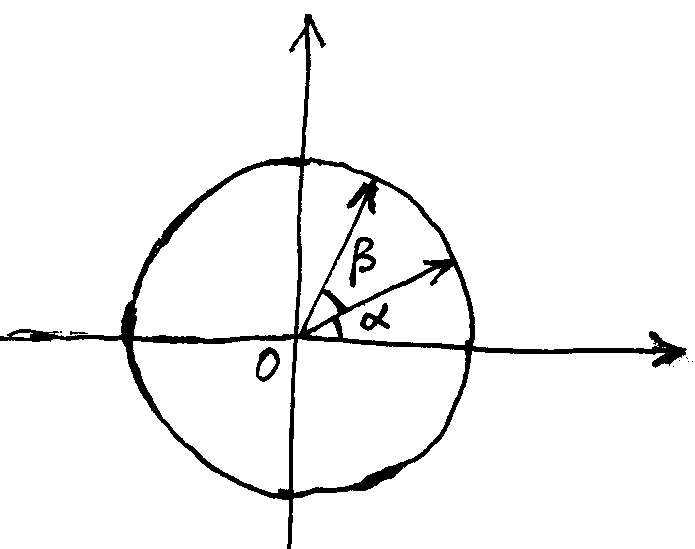
\includegraphics[width=4.5cm]{Preface/alphaplusbeta.png}
%\caption{default}
%\label{default}
\end{center}
\end{figure}


等式左侧(LHS):

\begin{eqnarray*}
(\cos \alpha + i \sin \alpha) \cdot (\cos \beta + i \sin \beta)  \\
 (\cos \alpha \cos \beta - \sin \alpha \sin \beta ) + i ( \sin \alpha \cos \beta + \cos \alpha \sin \beta)
\end{eqnarray*}

等式右侧(RHS):

\begin{equation}
\cos (\alpha + \beta) + i \sin (\alpha + \beta)
\end{equation}

因此:

\begin{eqnarray}
\cos (\alpha + \beta) &=& \cos \alpha \cos \beta - \sin \alpha \sin \beta\\
\sin (\alpha + \beta)&=& \sin \alpha \cos \beta + \cos \alpha \sin \beta
\end{eqnarray}

在物理学中,任何测量值都是一个实数,我们无法从“表盘”中读出个虚数来,但引入虚数,确实可给我们带来计算上的便利。

比如我们经常用$e$指数函数来表示一个波动:

\begin{equation}
\psi (x,t) = A e^{i (kx - \omega t)}
\end{equation}

这里相位是:

\begin{equation*}
k x - \omega t
\end{equation*}

对波动$\psi(x,t) =  A e^{i (kx - \omega t)} $,取固定相位,比如0,研究相位为0传播的速度,这就是相速度(phase velocity)。

\begin{equation*}
 k x  - \omega t = 0
\end{equation*}

对上式做微分,

\begin{equation*}
 k dx - \omega dt  = 0
\end{equation*}

于是得到相速度$v_p$:

\begin{equation}
v_p = \frac{dx}{dt}= \frac{\omega}{k} = \frac{2 \pi / T}{2 \pi / \lambda} = \frac{\lambda }{T }
\end{equation}

这里$v_p > 0$,表示波动是从左向右传播的,即沿着$x$轴的正方向传播。

但假如波函数是如下形式:

\begin{equation}
A \cos (kx + \omega t)
\end{equation}

解出来的$v_p < 0$,我们就说波动是从右向左传播的。


因为虚部的存在,$\psi (x,t)$本身并不直接对应物理量,但$\psi (x,t)$取实部

\begin{equation*}
\Re \psi (x,t) = A \cos (kx - \omega t)
\end{equation*}

就可以对应物理量了。比如机械波的振动,电磁波中电场分量或磁场分量的取值等等。


\subsection{直角坐标系}

我们回到本节一开始的思路,人对运动物体的研究是要借助凝视,或借助高速摄像机的。所谓高速摄像机就是对百万分之一秒($10^{-6}$s),甚至更短的时间间隔进行曝光。

借助于曝光时间很短,但又绝对不是0的高速摄像机,我们可以拍着胸脯说:我已经把我关心的运动都静态化了,或我们已经把它们——运动中的物体——冻结住了。至少可以在高速摄像机里成像了。

然后我们应如何描述它们呢?

物理学家的办法是建立一个坐标系,考虑到真实的世界是三维的,有前后、左右和上下的区别,我们选我们所在的地方为原点,然后以向右为$x$轴,向前为$y$轴,向上为$z$轴,这样我们就得到了一个三维的直角坐标系,也叫笛卡尔坐标系(cartesian coordinate)。笛卡尔(1596 — 1650)是与伽利略几乎同时的一位科学-哲学家。

我们把$x$轴、$y$轴和$z$轴想象为一根长长的尺子,我们需要在尺子上划分刻度,比如以米为单位。物体的位置可以用三个数($x, y, z$)来表示。

首先我们由物体的所在向$z$轴做投影,得到的就是$z$。然后我们由物体的所在出发吊一根铅垂线,得到物体在$x-y$平面上的投影($x, y$),然后再由这一点出发,向$x$轴做垂线,得到的就是$x$,向$y$轴做垂线,得到的就是$y$。

\begin{figure}[htbp]
\begin{center}
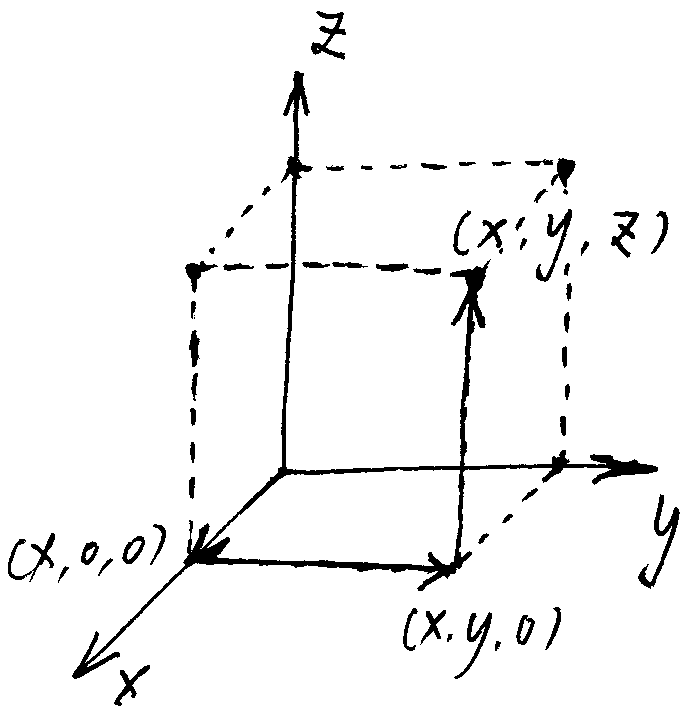
\includegraphics[width=5cm]{Preface/cartesianxyz.png}
%\caption{default}
%\label{default}
\end{center}
\end{figure}

对于大小可以忽略的物体而言,我们说出物体所在的位置,就算交待清楚了。比如:“在$t$等于0秒,物体的$x$取5米,$y$取3米,$z$取0米。”这可能是在描述我家里的玩具小汽车。

这个上下、左右、前后是怎么定的?

我们一般都说物理世界是各向同性的,是平移对称的,即我们在世界的不同地方,不论是巴黎、北京还是纽约,不论我们如何选取我们的坐标轴的取向,我们都会得到相同的物理规律。不同坐标系下,物理陈述的关系可以用一组数学公式描述,这个差不多就是研究相对论的出发点了。

这些当然都对。但我现在想说的是,如果一开始就这么“任意”,我们可能压根就不会得到三维直角坐标系这个概念。

当我们定下第一个三维直角坐标系的时候,上下、左右、前后还是有标准的。

上下:在地球表面上,因为重力的关系,向下落是物体的自然倾向,向上是需要解释的。

前后:人本身并不是前后对称的,眼睛长在脸的前面,所以我们只能向前看,向后看必须要扭脖子。

左右:这个比较难区分,假如你在一个小孩的左侧和右侧放上同样的好吃的,他有可能会真的往左动动,然后又往右,如此纠结、犹豫一番,才会扑向左侧或右侧的好吃东西。难归难,但对人而言,还是有区分左右的标准的,比如对普通人来说,右手会更强健有力一些。

比如我们可以这样:先定上下,用铅垂线;然后定东西,以太阳升起的方向;然后再定南北。或者也可以先定南北,借用北极星的方位。


\subsubsection{单位向量}

在笛卡尔坐标系中,物体的位置用矢量$r$表示,所谓矢量就是一个既有大小,又有方向的量,所谓方向和我们所处的三维空间有关,它来源于我们可以绕过,或跳过障碍物这类日常经验。

为了强调$r$是矢量,我们用符号$\vec r$表示。

我们现在来定义两个矢量的相加,比如:$\vec r_1 + \vec r_2$,它当然还是个矢量,并且应当满足交换律:

\begin{equation}
\vec r_1 + \vec r_2 = \vec r_2 + \vec r_1 = \vec r
\end{equation}

如果是讲数学的话,这就是个规定,不需要再多做解释。但如果是物理的话,我们会再多说几句,说这是先往$\vec r_1$的方向上走了$r_1$远,然后又沿$\vec r_2$方向走了$r_2$远,这么走的效果和先$r_2$再$r_1$的效果是一样的。

这里我们是在替物理挑一套合适的数学语言。这套数学的语言对经典力学而言,具体说是对经典力学里如何描述质点的运动而言,就是三维实系数的矢量空间。

三维实系数矢量空间中的任何一个矢量都可以按照平行四边形的法则进行分解。

\begin{equation}
\vec r = \vec r_1 + \vec r_2
\end{equation}

但有一种分解方式会比较方便,即$\vec r_1$和$\vec r_2$垂直的方式,在这种方式下,我们说$\vec r_1$中没有丝毫的$\vec r_2$的成分,同样$\vec r_2$中没有丝毫$\vec r_1$的成分。

这符合最佳分类的一般原则:

\begin{center}
既不重复,也不遗漏!
\end{center}

在$\vec r_1$方向上的单位向量是:

\begin{equation}
\vec i = \frac{\vec r_1}{r_1}
\end{equation}

在$\vec r_2$方向上的单位向量是:

\begin{equation}
\vec j = \frac{\vec r_2}{r_2}
\end{equation}

\begin{figure}[htbp]
\begin{center}
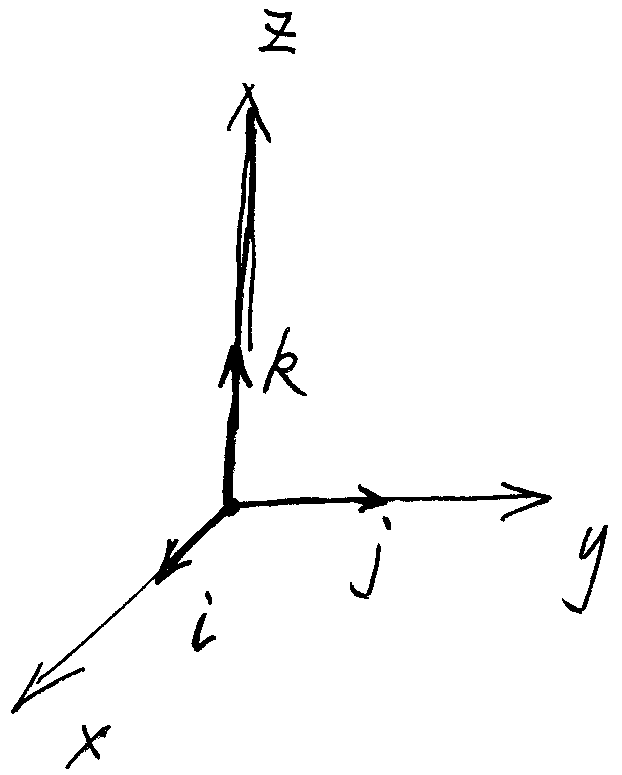
\includegraphics[width=4cm]{Preface/cartesian.png}
%\caption{default}
%\label{default}
\end{center}
\end{figure}

我们选取$\frac{\vec r_1}{r_1}$为$x$方向上的单位向量,记做$\vec i$;选取$\frac{\vec r_2}{r_2}$为$y$方向上的单位向量,记做$\vec j$。最后还剩一个$z$方向上的单位向量$\vec k$,我们通过矢量的叉乘(cross product)得到它。

\begin{equation}
\vec k = \vec i \times \vec j
\end{equation}

叉乘在这里需要满足右手法则,即:

\begin{enumerate}
\item 

伸出右手,除大拇指外其他手指指的方向是$\vec i$的方向;

\item

手指自然向手掌弯曲并握拳,手指弯曲后指的方向是$\vec j$的方向;

\item 

最后大拇指指的方向是$\vec k$的方向。

\end{enumerate}

利用叉乘,我们有更多$\vec i , \vec j , \vec k$的性质:

\begin{eqnarray}
\vec i \times \vec j & = & \vec k \\
\vec j \times \vec k & = & \vec i \\
\vec k \times \vec i & = & \vec j 
\end{eqnarray}

有了$\{ \vec i , \vec j , \vec k  \}$的定义,三维空间中的任何一个矢量$\vec r$都可以表示为$\vec i , \vec j , \vec k$的线性叠加。

\begin{equation}
\vec r =  \vec i  r_i +  \vec j  r_j +  \vec k  r_k 
\end{equation}

这就是说我们的分类(分成$\vec i , \vec j , \vec k$三类)并不遗漏,用数学的术语说,我们的分类是完备的。

\subsubsection{点乘和叉乘}

\begin{enumerate}

\item 

对两个矢量$\vec a, \vec b$,我们可以定义点乘(point product)

\begin{equation}
\vec a \cdot \vec b = a_i b_i + a_j b_j + a_k b_k
\end{equation}

矢量点乘的例子是做功,即“功等于力点乘位移”:

\begin{equation}
W = \vec F \cdot \vec l
\end{equation}

有一点必须提醒大家,因为矢量的记号里的这个箭头 \quad  $\vec {}$ \quad 写起来实在麻烦,所以我们经常会省去,前提是你心里要明白。实际上理论物理学的永恒主题就是发明记号,然后再简化记号。表面看起来很抽象,但其实都是为了方便。

\item

我们可定义矢量$\vec a$的模,即$\vec a$的大小$a$:

\begin{equation}
a = \sqrt{ \vec a \cdot \vec a } = \sqrt{ a_i^2 + a_j^2 + a_k^2 }
\end{equation}

\item

两个矢量$\vec a, \vec b$的叉乘(又叫矢量乘,因为这样乘出来是个矢量):

\begin{equation}
\vec a \times \vec b = 
\left(  
\begin{array} {lcr}
i & j & k \\
a_i & a_j & a_k \\
b_i & b_j & b_k 
\end{array}
\right)
\end{equation}

\end{enumerate}

进一步展开需要用到行列式的知识:

\begin{equation*}
\left(  
\begin{array} {lcr}
i & j & k \\
a_i & a_j & a_k \\
b_i & b_j & b_k 
\end{array}
\right)
= i 
\left(  
\begin{array} {lcr}
 a_j & a_k \\
 b_j & b_k 
\end{array}
\right)
- j
\left(  
\begin{array} {lcr}
 a_i & a_k \\
 b_i & b_k 
\end{array}
\right)
+ k
\left(  
\begin{array} {lcr}
 a_i & a_j \\
 b_i & b_j 
\end{array}
\right)
\end{equation*}

$= \vec i (a_j b_k - a_k b_j) - \vec j (a_i b_k - a_k b_i) + \vec k (a_i b_j - a_j b_i)$

矢量叉乘的例子是力矩$\vec \tau$和角动量$\vec J$等:

\begin{eqnarray}
\vec \tau &=& \vec r \times \vec F \\
\vec J & = & \vec r \times \vec p
\end{eqnarray}


\subsubsection{左手系和右手系}

在物理里面经常会讲左手系和右手系,这个是这样来定的。

伸出你的右手,大拇指向上,剩下的那些手指头做出一个自然向“手掌”握的动作,大拇指的指向是$z$轴的正向,剩下手指头初始指的方向是$x$轴正向,自然握的方向是$y$轴正向。

这样规定的$xyz$坐标系就是右手系,我们在物理里一般都用右手系。

\begin{figure}[htbp]
\begin{center}
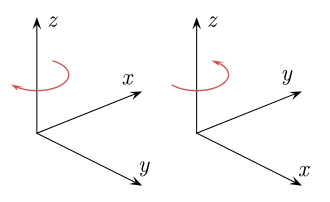
\includegraphics[width=7cm]{Preface/lefthandrighthand.png}
\caption{左图为左手系;右图为右手系。}
%\label{default}
\end{center}
\end{figure}

当然还有左手系(伸出你的左手……),左手和右手的关系好像是照镜子,比如:一个物体在右手系中的坐标是($5, 3, 0$),那么它在左手系中的坐标则可能是($5, -3, 0$)。

对纯平面的东西是没必要分左手和右手的。

比如我拿一张白纸,在纸上画一个向右转的箭头,这个看上去是和向左转的箭头正好相反,但只要你把白纸转过来,你就会发现它其实同时也是个向左转的箭头。

但对三维结构,一个右手的螺旋上升,就没有办法通过一个在三维空间中的重新摆放和定位变成一个左手的螺旋上升。或者更简单的例子:左手握成一个拳头,右手也握成一个拳头,无论我们怎么摆放它们,它们都不可能完全一样。

还是拿一张白纸,我们画一个逆时针旋转的箭头,即面对我们,箭头是向左的,我们再假想这实际上是个三维结构,它是穿过纸面向我运动的。然后我们再把白纸翻转过来,这时固然我们看到的是一个向右转的箭头,或是一个顺时针旋转的箭头,但不要忘记这时这个旋转的箭头已经是穿过纸面远离我运动的了,这就是一个具有右手手性的螺旋。而且随便我们摆放它,这个结构都是个右手手性的螺旋。

DNA双螺旋和蛋白质的$\alpha$螺旋都是有手性的。

\begin{figure}[htbp]
\begin{center}
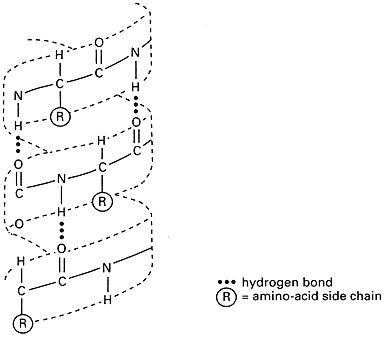
\includegraphics[width=7cm]{Preface/alphahelix.jpg}
\caption{$\alpha$螺旋示意:由于“CO-NH”结构的存在,我们是可以在链上对$\alpha$螺旋定义走向的,它自然是有手性的。}
%\label{default}
\end{center}
\end{figure}


在光学中的例子则是左旋光和右旋光。

\begin{figure}[htbp]
\begin{center}
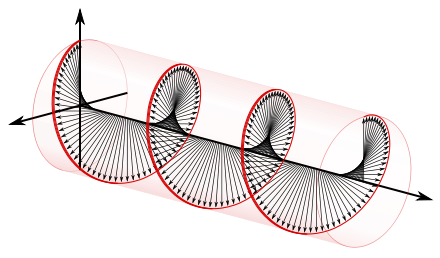
\includegraphics[width=10cm]{Preface/circularpolarization.png}
\caption{按照我们的定义这是一个左旋光}
\label{default}
\end{center}
\end{figure}


\subsection{左旋光和右旋光}

光波就是电磁波,是特定波长(400-700nm)能被我们人眼所见的电磁波,光波传播的方向和光波电分量振荡的方向垂直,光波电分量振荡方向可以是在一个方向上,比如说就固定在$x$方向上,这就是线偏振光,它也可以边振荡边旋转,比如边振荡边往左(或右)转,这就是圆偏振光了。

左旋光或右旋光可以这么定义,假设光是冲着我们传播的,如果电分量是边振荡边向左转就是左旋光,否则就是右旋光。

电磁波是电场$E$和磁场$B$在时间和空间中的传播。它有如下性质:

\begin{enumerate}
\item 

电磁波是横波,电场和磁场振动的方向都和电磁波传播的方向垂直。

电场振动方向$\vec E$,磁场振动方向$\vec B$和电磁波传播的方向$\vec k$,正好构成右手法则。

\item 

根据电磁学的规律。变化的电场会感生变化的磁场,而变化的磁场又会感生变化的电场。

原则上我们只要给出电场$\vec E$随时空的传播,就决定了磁场$\vec B$随时空的传播。

\item

现在我们只需要研究电场$\vec E$随时空的传播。

如果我们选取电磁波传播的方向是$z$轴的正方向的话,电场$\vec E$就在$x-y$平面上。

假如$\vec E$就在$x$轴上,我们说电磁波是$x$-偏振的,因为电磁波就是光波,所以对光来说我们也有$x$-偏振光。

角频率为$\omega$的$x$-偏振光的电场分量就可以表示为:

\begin{equation}
\vec E (z, t) = \vec {e_x} E_0 e^{i ( kz - \omega t ) }  
\end{equation}

这里$\vec {e_x}$表示$x-y-z$坐标系中沿$x$方向的单位矢量。

类似地,我们还可以写出$y$-偏振光的电场分量:

\begin{equation}
\vec E (z, t) = \vec {e_y} E_0 e^{i ( kz - \omega t ) }  
\end{equation}

由于$\vec {e_x}$和$\vec {e_y}$垂直,所以$x$-偏振光里一点$y$-偏振光的成分都没有。反过来说,$y$-偏振光里一点$x$-偏振光的成分都没有。

\item

所谓自然光就是各个方向的偏振光都有,每个方向偏振光的强度都是一样的。

\item

那么圆偏振光如何表达呢?

圆偏振光里面的电场矢量$\vec E$是旋转的,可能向左转,也可能向右转。

$\vec E$在$x$轴的投影:$ \frac{1}{\sqrt{2}} E_0 \cos \theta$

$\vec E$在$y$轴的投影:$ \pm  \frac{1}{\sqrt{2}} E_0 \sin \theta$

如果取正号($\pm$中上面的“+”),($ \frac{1}{\sqrt{2}} E_0 \cos \theta$, $ \frac{1}{\sqrt{2}} E_0 \sin \theta$)正好构成一个向左旋转的圆,或说是逆时针的。(称之为左旋光)

如果取负号($\pm$中上面的“-”),($ \frac{1}{\sqrt{2}} E_0 \cos \theta$, $ - \frac{1}{\sqrt{2}} E_0 \sin \theta$)正好构成一个向右旋转的圆,或说是顺时针的。(称之为右旋光)

考虑到正弦/余弦函数具有如下性质:

\begin{eqnarray*}
\cos (\theta + \pi /2 ) &=& - \sin \theta \\
\cos (\theta -  \pi /2 ) &=& \sin \theta
\end{eqnarray*}

对向左旋转的电矢量,电矢量的$x$分量和$y$分量分别为:

\begin{eqnarray*}
E_x &=& \frac{1}{\sqrt{2}}  E_0 \cos (k z - \omega t) = \frac{1}{\sqrt{2}}  \Re E_0 e^{i (k z - \omega t)}  \\
E_y &=& \frac{1}{\sqrt{2}}  E_0 \cos ( - \pi /2 +  kz - \omega t  ) = \frac{1}{\sqrt{2}}  \Re E_0 e^{ - i \pi /2 } e^{i (kz - \omega t)} \\
{} &=& \frac{1}{\sqrt{2}}  \Re E_0 (-i) e^{i (kz - \omega t)} 
\end{eqnarray*}

类似地,我们可以写出向右旋转的电矢量,表示为:

\begin{eqnarray*}
E_x &=& \frac{1}{\sqrt{2}}  E_0 \cos (k z - \omega t) = \frac{1}{\sqrt{2}}  \Re E_0 e^{i (k z - \omega t)}  \\
E_y &=& \frac{1}{\sqrt{2}}  E_0 \cos ( \pi /2 +  kz - \omega t  ) = \frac{1}{\sqrt{2}}  \Re E_0 e^{ i \pi /2 } e^{i (kz - \omega t)} \\
{} & = & \frac{1}{\sqrt{2}}  \Re E_0 i e^{i (kz - \omega t)} 
\end{eqnarray*}

这么写太啰嗦了,我们把它们写精炼一些,

向右旋转的光:

\begin{equation}
\vec E = \frac{1}{\sqrt{2}} E_0 \Re \left(
\begin{array}{c}
1 \\  i
\end{array}
\right) e^{i (kz - \omega t)}
\end{equation}

简单说电场矢量$\vec E$在$y$方向上的振动比$x$方向上的振动超前$\frac{\pi}{2}$。

向左旋转的光可写为:

\begin{equation}
\vec E = \frac{1}{\sqrt{2}} E_0 \Re \left(
\begin{array}{c}
1 \\ - i
\end{array}
\right) e^{i (kz - \omega t)}
\end{equation}

电场矢量$\vec E$在$y$方向上的振动比$x$方向上的振动要落后$\frac{\pi}{2}$。

类似于$x$-偏振光和$y$-偏振光,向左旋转的光和向右旋转的光也是完全不相容的。

即:左旋光里没有任何右旋光的成分,右旋光里没有任何左旋光的成分。

据说现在3D电影使用的就是左旋光和右旋光,因为用线偏振光有个大毛病,假如左眼看$x$偏振光,右眼看$y$偏振光,我们的脑袋稍微晃一晃,左眼眼镜里偏振片的方向会与$x$方向形成夹角,这样$y$偏振光也能进来一部分了,于是电影的图像就会模糊。

左旋光和右旋光没这个问题,因为它是向左转和向右转的关系,与偏振片本身在空间中的方位无关。所以我们可以让左眼总看到左旋光,而右眼总看到右旋光。


\end{enumerate}



\newpage

%\input{TheReal/Aether}

\section{从天球的音乐到玻尔模型}

形或古希腊人所说的“idea”,有多种含义,比如:形状,这是和视觉有关的;比如风格、分类,这可以是和视觉有关的,也可以无关,比如音乐也可以有风格,这就是和声音有关的了。

和视觉有关的“形”是直观的,我们无须论证,纠结于如何用语言表达,仅凭图形——或者是静态的,或者是想象中动态的——直接给出结果。对形的研究会导向几何学,几何本身是视觉的,而视觉是偏好静的,偏好不动的,但一加“学”,几何“学”或“学”几何就动起来了。

我们如何学呢?或者演示,用圆规和直尺,或者像毕达哥拉斯那样拿根木棍面对沙土,世界是一步一步地被展现出来的,一笔一划本身就是个动态的过程。我们努力说:“首先如何,其次如何,然后,又然后……”

所谓动态就是次序,我们首先只关注首先要解决的,其次,带着对刚刚过去的对首先的记忆,探讨紧接着要解决的问题,我们的思想没法分叉。人在专注的状态下,视觉也需要一个焦点。当我们的视觉遭遇挑战,看不清某物的时候,我们凝眼观瞧,把视线使劲聚焦于某物,凝眼就是凝神,不受诱惑地专注于某物,看清楚一点再继续看下一点。

这个结构很像自然数:“0,1,2,3,……”,一步一步地展示给你看,比如“我是如何用直尺和圆规作图的”,这种线性展开的结构就是时间,“学”的过程,对学的人是学,在Challenge,对展示的人来说是在“证”,在说服,这个过程是世界次第展开的过程,是叙事、是Chronicle。

\subsection{形与声}

“学”依赖语言,语言是一种声音现象。

据说人能够发出一个八度再加一个四度的声音。

古代世界,天和地很近,音乐和人也很近。孔子闻韶乐“三月不知肉味”,这种沉浸在声音里的境界和我们今天听流行音乐,把音乐当做一种背景噪音,是完全不同的两种声音技术。今天我们听音乐往往是为了抑制我们心中的背景噪音。

古代的音乐都很简单。简单到好比就是敲击单音音叉发出的声音,单音音叉是校音用的,它在古代世界的对应物是中国的黄钟律管或希腊的单弦琴(Monochord)。它们发出很纯的音,基本上就是一个频率。孔子一生关心礼,礼与乐相联,乐就是音及音的混杂与排列。

我们用音高,频率,响度,音色等来描述声音。音高就是频率,是描述“音”诸参数中最重要的一个。人天生就是一个感知音高的灵敏动物,高音激越,使人振奋,低音呜咽,让人伤感。简单的音乐庄重使人入静,而复杂多变的音乐也如一场“视觉的盛宴”,它使我们好奇和沉迷。

听觉和视觉一样,是感觉,同时也是思维,我们的眼睛和耳朵接受信息,同时也处理、歪曲信息以为我们所用。古代的政治传统,古代的教育家都注重音乐教育,这其中最重要的就是对音乐体系的保留和传承。

比如唱歌的时候要先定调,调可以定低点,显得庄重,也可以定高点,显得轻快。定好调后,一系列的声音次第展开,它们的相对音高保持一个固定的结构,比如:

“低,低低,高,高高,低,中中,……”

在给定乐谱的前提下。基准音高的选取,或所谓定调是任意的。我们可以定高点,无非大家唱不上去而已。但因为有人唱不上去,这个定调就也不是完全主观任意的了。

古代政治秩序大多由推崇勇猛进取精神的战士集团建立,对战士共同体而言,最重要的是要保持这种勇猛进取的精神,能够保持这种精神的音乐会与特定音高有关,这是人群的共同经验。比如柏拉图在《理想国》中就说,要摒弃悲伤和软绵绵的吕底亚调和伊奥尼亚调,而推崇多利亚调和佛里吉亚调。

保持这种对声音的共同经验在古代政治传统中是非常重要的,其中之一就是确定音调,或基准音的频率,然后在此基础上给出其他音的定义,其他音是相对于基准音而言的,可以更高,也可以更低,构成一个阶梯状的结构。

原子的“idea”是无所不在的,这里由人的听觉经验,我们再次得到了原子的概念,即存在着“音高”的原子,进一步细分不同音高的原子是没有必要的。

保存音乐制度最简单的方法就是造一套标准的乐器,然后后人反复向这些标准的乐器学习,第一套自然是由城邦的缔造者“铸造”的。

考虑到弦乐器与弦绷紧的程度有关,受湿度、温度影响较大,青铜器制造的发音器会是理想的选择,这是为什么“钟”会成为“国家”符号的原因,塔可夫斯基电影《安德烈·卢布廖夫》再现的是俄罗斯帝国创旦的精神基础,在影片的结尾就出现了工匠之子铸钟的奇迹。

\begin{figure}[htbp]
\begin{center}
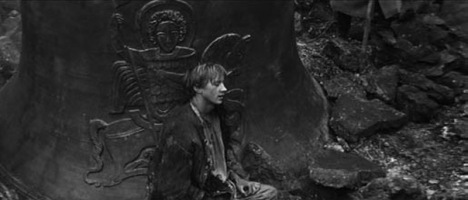
\includegraphics[width=8cm]{Preface/st_george_bell.jpg}
%\caption{default}
%\label{default}
\end{center}
\end{figure}

钟是要发音的,音高是有标准的,“音高”高一些,低一些,很微妙,但人的耳朵,或某些人的耳朵天生就是辨别音高的灵敏仪器。只有能发出特定音高的钟才是可以被接受,一只发音不准的钟在敲响的时候不嘹亮,不能激发人民激越的精神,这对城邦是不利的。

这里有个似是而非但很有趣的讨论,人有时间感,但人的时间感是非常内在的,几乎不存在什么可以相互交流的基础。这是妨碍人产生运动观念,并研究运动的重要原因。音高即频率,频率就是时间的倒数,人没法准确标记时间的流逝,但人却是辨别频率(时间倒数)的精密仪器。同时我们的发音器官,还能娴熟地对不同音高的声音进行模仿,这是我们具有语言和音乐能力的生物学基础。

类似地,我们还可以讨论视觉,讨论视觉对位置和速度的分辨。人天生就能在相当精确的意义下辨别位置,但我们对速度的判断就要差许多。我们说A比B快,其实是通过位置下的判断,即AB同时出发,但A先撞线,所以A更快。这是亚里士多德无法得到“正确”的落体规律的原因,他受人本身的局限,速度是很难直接被看的。

古代实验技术还没有充分发展起来,而实验技术的充分发展与资本主义的生产方式兴盛有关,近代自然科学与资本主义生产方式同步爆发并非巧合。回顾二者,科学史和资本主义发展史,两者讲的是同一个故事,只是叙事的角度生了变化。

由“造钟”故事,我们得到一个新洞见,即:“音与形有关”。对钟来说这是大大地简单化了,因为材质也很重要,但形状确实决定了钟振动的频率。这意味着:“听音可以定形,定形可以定音”。

形既是形状也是模型,还是形式。在毕达哥拉斯和柏拉图的传统里,形是与数紧密相连的。比如钟的形由何而定呢?长、宽、高、是数字,钟的厚度也是数字,但这一堆数字的集合又有什么意义呢?

当我滔滔不绝地罗列一堆数字的时候,这是没有意义的。我们需要给出数字和数字之间的关系,才有意义。而且最好是只给出一个关系(或最少关系),就能让所有的数字各就各位。找到这样的规律自然是对思维的奖励,是可以向众人夸耀的;同时这也是技术,有了技术我们就能铸钟,小孩的父亲是会铸钟的,但他把技术带到坟墓里去了。

《安德烈·卢布廖夫》中的小孩是幸运的,他必须试试,他也只能试试。在拜占庭衰败之后,东正教来到了俄罗斯与当地的土豪、愚民混合,文明在绝望中重新开始,这就是俄罗斯的宿命。卢布廖夫受不会铸造但却造出钟的小孩的激励,重新拿起画笔开始画注定会塑造俄罗斯民族精神的那些很平、很抽象圣像画。

\begin{figure}[htbp]
\begin{center}
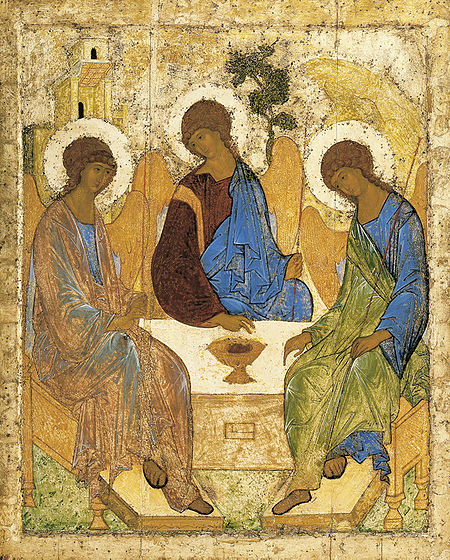
\includegraphics[width=8cm]{Preface/RublevTrinity.jpg}
\caption{卢布廖夫的《三圣像》}
%\label{default}
\end{center}
\end{figure}

画是形(idea),音是声(logos)。形和声都能塑造性格,前提是我们生活在某种生活中,或我们生活在某种历史中。

\subsection{数字与和谐}

“几何学”(Geometry)是对形的规定,而“和声学”(Harmonics)是对音的规定。所谓规定就是数字之间的联系,最简单的数字和数字间的联系是“相等”,稍微高级点的是比例,是合乎比例。

比如人脸,人脸上五官的位置和尺寸是需要合乎比例的,这种合乎比例是我们天生可以判断的,但很难用数字说清楚。近一二十年随着计算机对数据处理能力的提高和神经科学的进步,在这方面有了很多具体技术的进展。

比例或合乎比例会产生美,这是某种审美观念下的模式识别。比如古代东夷部族以扁头为美,甚至不惜把小孩的头骨弄扁以合乎比例。这个习俗在今天还有遗存,不少地方有端正小孩睡姿以把头睡扁的说法。

在音乐中我们很容易发现音高与数字的关系。这是毕达哥拉斯的贡献。音乐的历史一定很古老。在毕达哥拉斯之前人类就有音乐了,不但有音乐还有规定音高的一套体系,即有一套术语来说清楚“不同音高”的音之间的关系。

比如当我发出一个音后,让你发出一个高四度的音,你就能发出这样一个音,并得到我的认同。这套语言游戏能够玩儿的起来。这些当然都是基于感官经验讲的,本来和数字没啥关系。传说毕达哥拉斯在路过铁匠铺时,受到叮叮当当声音的启发,回去研究各种乐器的音高,比如弦乐。

所谓弦乐器就是一根绷紧的弦,两端固定,中间可以快速振动起来,扰动空气发出声音,弦乐的频率自然就是琴弦发出的声音。这是典型的机械振动的问题,弦上会有波动,但因琴弦两端是固定的,所以波传播不出去,它只能被限制在琴弦上振动,并整体具有一个轮廓,琴弦就在这个轮廓内振动,这种振动叫驻波。

琴弦上的振动是波动,当一列波从左向右传播时碰到弦的端点会反射回来,驻波就是两列相向传播的波的叠加:

\begin{equation}
\frac{A}{2} \left( \cos ( kx - \omega t ) + \cos ( kx + \omega t ) \right) = A \cos kx \cos \omega t
\end{equation}

这里A是振动的幅度,振动的轮廓线是:

\begin{equation}
A \cos kx 
\end{equation}

$k = \frac{2 \pi}{\lambda}$是波矢,$\lambda$是波长,因为琴弦的两端已经被限制住了,琴弦的长度$L$可以取半波长,一个波长,一个半波长,……,简单说就是半波长的整数倍:

\begin{equation}
L = \frac{n \lambda}{2}, n = 1, 2, 3, ...
\end{equation}

波长可以表示为:

\begin{equation}
\lambda = \frac{2L}{n}
\end{equation}

这就是合乎比例。

考虑到弦上波速$v$是个常量,频率可以表示为:

\begin{equation}
\nu = \frac{n v}{2 L }
\end{equation}

给定弦长$L$,只有这样的波动,或这样波动的叠加才可以存在。进一步讲,如果我们考虑一个符合两端被限制住的琴弦的一般运动,这个一般运动总是可以被分解为一系列不同$n$取值的,波长为$\lambda_n = \frac{2L}{n}$,频率为$\nu_n = \frac{n v}{2 L }$的振动的叠加。

\begin{equation}
\sum\limits_{n} A_n \cos \frac{n \pi x}{L} \cos \frac{n \pi vt}{L}
\end{equation}

我们管$n = 1$的音叫做基音,这个频率$\frac{v}{2L}$的声音是最主要的,但弦上也会有$n= 2, 3, ...$的成分,这些音叫做泛音。

拨动长度$L$的琴弦,我们听到的是基因和泛音的混合,最主要的是基因,频率为$\nu_1 = \frac{v}{2L} $,其次是第一个泛音,频率为$\nu_2 = 2 \nu_1$,它们之间是1: 2的关系。

假如我们把琴弦的长度减半,其实就是用手在弦长的一半按住琴弦,此时我们会有新的弦长$L/2$,同时新的基因频率$2 \nu_1$,但此时,因为弦长只剩下一半了,我们拨动琴弦发出的声音里就没有$\nu_1$的成分了。

听起来的感觉是这样的,首先$L/2$琴弦发出的音和$L$琴弦发出的音很像,其次$L/2$琴弦发出的音当然要比$L$琴弦发出的音要高,这就好比是一个人沿螺旋形的楼梯升高,每个台阶都对应一个特定音高的音,在螺旋式升高了几个音之后我们又回到了起始位置,只是高了一些,我们还可以继续螺旋升高,每提升一个台阶都会感觉和曾经的某个台阶很像,只是更高了。

在音乐理论里,我们管这个结构叫“八度”,当音高由$\nu_0$提高一倍到$2 \nu_0$的时候,我们就说“升了八度”。类似地,当音高由$nu_0$降一倍到$\nu_0 /2$时,我们就说“降了八度”。我们一般能发出一个八度再加一个四度的音。

\subsubsection{毕达哥拉斯的和声学}

毕达哥拉斯研究了音和形的关系,并发现这个关系可以被数字精确地描述。比如我们刚刚讨论过的,当弦乐器的弦长比是1:2时,频率比是2:1,正好对应音乐理论中的“八度音程”。

八度关系本来就存在于音乐实践中,属于人的日常经验。现在发现“一个八度”可以表示为精确的数字比1:2,这个数字比其实是对形的描述。只是因为这里弦是一维的,我们对形的描述比较简单。

一个日常经验可以对应于一个数字的比例关系是足够让人兴奋的,毕达哥拉斯讲“万物皆数”,其实讲的是“万物皆合乎比例”。只有合乎比例,万物才能存在,只是这些比例有待我们的发现。

合乎比例是个静态的世界观。

除了1:2,毕达哥拉斯还发现当弦长比是2:3时,音的关系是音乐理论中的五度音程。而弦长比是3:4时是音乐理论中的四度音程。毕达哥拉斯只发现了这几个关系。它足够优美,但还不足以解释音乐理论中所有的音。但这已经足够他嘚瑟的了。

更重要的是他开辟了一个用数字、用比例关系去研究音乐的方法,进而是研究整个宇宙万物的方法,可以说今天的理论家都是毕达哥拉斯的信徒。

\begin{figure}[htbp]
\begin{center}
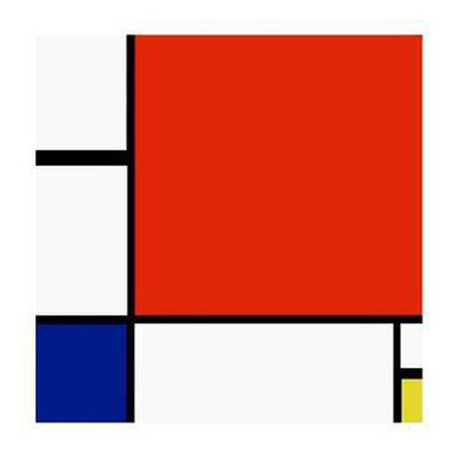
\includegraphics[width=5cm]{Preface/colorsquare.jpg}
\caption{蒙德里安的作品是“万物皆数”、“整体和谐”观念在绘画领域的实践。}
%\label{default}
\end{center}
\end{figure}

毕达哥拉斯方案的缺陷是他被简单数字迷住了,1:2,2:3,3:4确实解释了八度音程、五度音程、和四度音程。但再要想把人对声音的感官经验——极其灵敏的感官经验——和简单数字比(m:n)建立关系就很困难了。

根据近代的十二平均律,我们在八度音程里面做12均分,这个均分是合乎比例地分——作为人,我们当然是凭我们的耳朵来分,这里我们必须赞叹人听觉器官的精密——我们要找到某个合适的比例因子$q$,使得:

$1 \nu_0$,$q \nu_0$,$q^2 \nu_0$,……$q^{12} \nu_0 =2 \nu_0$

因此:

\begin{equation*}
q = 2^{\frac{1}{12}}
\end{equation*}

这里难的是对2开12次方,$\sqrt{2}$就已经是无理数了,即$\sqrt{2}$就已经没办法表示成一个简单数字的比例了!这是毕达哥拉斯方案失败的原因。

我们解出:$q \approx 1.059463 $,并制表:

\begin{table}[htdp]
\caption{十二平均律}
\begin{center}
\begin{tabular}{|c|c|}
\hline
n & $q^n$\\
\hline
0 & 1 \\
1& 1.059463 \\
2 & 1.122462 \\
3 & 1.189206 \\
4 & 1.25992 \\
5 & 1.33484 \\
6 & 1.414213 \\
7 & 1.49831 \\
8 & 1.5874 \\
9 & 1.6818 \\
10 & 1.7818 \\
11 & 1.8877 \\
12 & 2 \\
\hline
\end{tabular}
\end{center}
\label{default}
\end{table}%

四度音程对应的弦长比是3:4,计算出来的频率比是:$\frac{4}{3} = 1.33333$,对应十二平均律表格中是$n = 5$的情形,可见:$1.33484$和$1.33333$相当接近。五度音程对应的弦长比是3:2,频率比是:$\frac{2}{3} = 1.5$,对应十二平均律是$n=7$,$1.49831$和$1.5$也很接近。

\subsection{天体音乐}

音乐与舞蹈相联系,古人总是载歌载舞,而载歌载舞是对“天”,对想象中“绝对秩序”的模仿,通过模仿来表达对“天”和人格化的“天”——神的亲近和虔敬。

根据古人的观念,天是天球,有几重天球,离地球最远的是恒星天,它们构成了一个背景,一个不动的背景。还有行星,“金木水火土,太阳和月亮”,它们相对于不动的背景穿行。每个行星都有自己的天球,以自己独特的方式运动。

天体运行的很慢,在没有灯光污染的古代,天体运行是很合适的研究对象,对恒星而言就是绘制星表,把所有可见的,相对而言都不运动的那些恒星的方位表达出来,所谓方位就是方向,所有恒星离我们是一样远的,它们居于最外层的天球。

在这种叙述下,每个恒星对应一个倾角$\theta $和一个方位角$\phi $,我们需要某种制图技术把天球上的恒星投影到平面上,这种制图技术和制作世界地图的技术没有什么区别。我们得到的星图,简单说就是诸星座。

恒星天以下还有土星天球,木星天球,火星天球,太阳天球,金星天球,水星天球和月亮天球。这是按照由外到内的次序,月亮天球离我们最近,月亮之下就是凡俗世界了(月下世界),万物变化不定,没有规律。但自月亮天球及以上就是神圣的所在,天球庄严地运转,超脱于朽坏和变化,被神圣的数学描述。

数字关系是不朽的,诸天也是不朽的,研究天体运行是研究数学,即像毕达哥拉斯在音乐中曾经找到的,找到简单的比例,天球的运行需要合乎比例,并作为一个整体和谐地存在,所谓和谐就是和声(Harmonics)。

这是“万物皆数”观念在天文学中的运用,古希腊的哲学家们已经能够计算太阳的大小,月球的大小,太阳和地球的距离,以及月亮到地球的距离,各个行星运转的周期等等。在他们的眼里,宇宙整体是一个和谐的存在:诸天各有各的半径,这是宇宙的形,而诸天各以不同的速度运转将会发出声音,速度越快音高就越高,月音低沉,土星离地球最远,运行最快因此土星音也是最激昂的。

传说乐器是阿波罗神给人的礼物,它是理性的象征,乐器因形的合乎比例而发出和谐的声音,和谐的声音使人的心灵柔和、敏感,function well成为一架理性的机器。

据柏拉图的《蒂迈欧篇》,宇宙是造物主理性的设计,在比喻的意义下,我们把宇宙想象为一把里拉琴,诸天的位置对应弦上不同的位置。我们无法想象这天体的音乐是不合乎比例的,虽然我们谁都没有听过天体的音乐(天籁之声),但诸天发出的音乐,有的如男低音,有的如男高音,又有的如女低音,有的如女高音。并整体符合某种比例,某种和谐关系。就好像毕达哥拉斯发现的弦乐中的1:2:3:4。

\begin{figure}[htbp]
\begin{center}
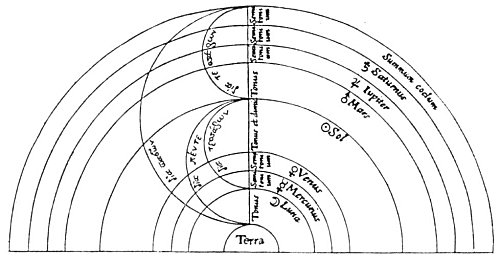
\includegraphics[width=11cm]{Preface/planetoctave1.jpg}
\caption{天体音乐的一种构想:最大圆弧表示八度音程,向下是两个四度音程,从地球向上还有个五度音程,并与从恒星天向下的四度音程正好重合。频率比由高到低是:$2: \frac{3}{2} : \frac{9}{8} : 1$。(根据一本中世纪手抄本的插图绘制,收入O. Pederson, M. Pihl: Early Physics and Astronomy, 1974。图6.1)}
%\label{default}
\end{center}
\end{figure}

这里整体和谐的思想是首要的,它或者体现为音乐的悦耳清晰(比如孔子的“三月不知肉味”),或者干脆就体现为一种数学关系的简单和优美(比如毕达哥拉斯的“1:2:3:4”)。人对音乐的欣赏和想象是可以闭上眼睛进行的,任随自己的思绪伴随着音乐的节奏奔跑,这就摆脱了日常经验对思维的限制,成为一种纯内在的,只与不朽的形式相关的理性思维。

西塞罗在《国家篇》中让西庇阿梦见自己身处宇宙之中,听到:

“由各个天体自身的运动和冲击产生出声音,这种声音是那些按恰当比率严格区别开来的各个不相等的音程划分出来的;它由高音和低音混合而成,将各种不同的和音造成统一的音程;……在处于最高点的星天(恒星天)历程上,那里的运动无比地迅速,就发生尖锐的快速的声音;而月球的历程(那是最低的)则以厚重的声音运动着;”

我们谁都没有听到过天体发出的音乐,西塞罗说这是因为我们从小听习惯了,反而听不见了。毕达哥拉斯的说法更高明,他说除了他自己谁也听不见天体的音乐,毕达哥拉斯说:

“他既不创作也不演奏任何人类演奏的那种竖琴或歌的旋律,而只使用一种神秘的、莫测高深的神圣方法,全神贯注于他的听觉和心灵,使他自己沉浸在流动的宇宙谐音之中。……只有他才能听到并理解这种谐音,以及由这些天体激发起来的和声。”

毕达哥拉斯的高明之处在于点明依靠感官——耳朵——是听不见“天体音乐”的,他需要的沉思,即:全神贯注于听觉和心灵,使自己沉浸在流动的宇宙谐音之中。类似地,柏拉图在《理想国》中嘲笑“仰望星空者”是观星迷,并摆明他自己研究天文学的方法是几何学。

研究天文学也并非是简单地应用数学-几何学,按照柏拉图的说法,研究是要发现理念,现象被理念(光)照亮,新的理念就是新的形式,就是新的类。换言之就是要发现具有表现力的新的数学-几何学。

西庇阿之梦是西方艺术中的常见母题,往前自然是毕达哥拉斯的“天体音乐”和柏拉图的“厄尔神话”,往后则是比如库布里克的《2001太空漫游》。

影片开始的时候,节奏非常缓慢,人(猿)生活在自然中,直到他们凭视觉洞见了一个抽象的几何形体从天而降,这是对几何学起源的神话式描写。在“数学-几何学”光芒的照耀下,镜头一转人类就进入了太空时代。

\begin{figure}[htbp]
\begin{center}
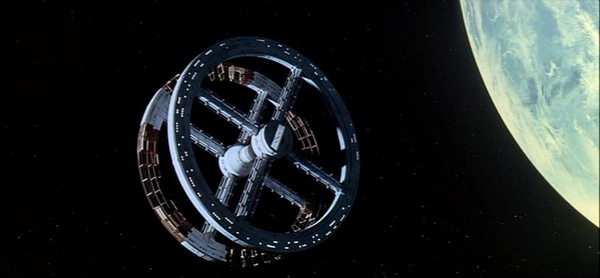
\includegraphics[width=10cm]{Preface/2001space.jpg}
\caption{2001太空漫游}
%\label{default}
\end{center}
\end{figure}

这就是理性的力量,但首先你需要像那只人(猿)一样被理想的几何打动,为之着迷,这就像毕达哥拉斯发现1:2:3:4可以解释音程一样,瞬间被理性的力量击中并宣称“万物皆数”!

而当影片即将结束的时候,我们看到类似西庇阿之梦的梦境,变换的色彩,抽象的几何形体,流动冲撞,这其实是对天体音乐的视觉再现。而随之进入的是更为具象的人类生活,所有美好或可以激发起美好与和谐感觉的画面,西方历史中值得尊敬和记录的种种视觉切片。

向伟大的西方文明致敬!

从毕达哥拉斯和柏拉图始到太空时代终,影片推出的1968年正是人类进军太空的最高潮,一年后的1969年人类首次登月成功。

在影片即将结束的时候我们听到的是《蓝色多瑙河》。

(从几何形体到《蓝色多瑙河》都是最常见的西方文明的符号。)


\subsection{开普勒}

开普勒是位承前启后的人物,一方面他和托勒密、西塞罗一样醉心于天体音乐的概念,希望能够发现宇宙整体和谐的规律,另一方面他关于行星运动的三个定律直接导致了牛顿的经典力学。

在牛顿的体系里万有引力$F = G M m /r^2$和牛顿第二定律$F = ma$取代了整体和谐,微分和积分取代了数字之间的合乎比例,运动的轨迹取代了静态的天球。

托勒密是古代天文学的集大成者,托勒密天文学的核心是匀速圆周运动,他把行星的运动分解为数个匀速圆周运动的叠加,并很好地与当时的天文学观测数据吻合。这是一种描述性的理论,表面看起来简单,但进入细节后就会觉得很繁复。即便是今天,我们也很难凭脑子去想哪怕是几个匀速圆周运动的叠加。

\subsubsection{开普勒的天球理论}

从整体和谐的观念出发,就需要找到更简单清晰的数学规律,具体说就是某种比例关系。开普勒的出发点和毕达哥拉斯很类似,都是整数。

在开普勒的年代,哥白尼的体系已经逐渐为天文学家接受,太阳不再是行星,地球取代了它的位置。已知行星按距离太阳由近到远排列是:水星、金星、地球、火星、木星和土星。

它们的轨道半径比是:

\begin{center}
8:15:20:30:115:195
\end{center}

为什么太阳有6颗行星,不多不少正好6颗,而它们的半径比又正好是以上的整数比?

今天看来开普勒的问题是完全没有意义的,因为根据万有引力定律,行星实际上可以出现在距离太阳的任何距离上,而今天已知的大小行星的数目也远远超出6颗。换句话说,开普勒的问题只有放到“整体和谐”观念下才有意义。

柏拉图在《蒂迈欧篇》中曾用四种正多面体与“水气土火”四种元素对应,但实际上有五种正多面体,这让人感到很不完美。

现在开普勒把五种正多面体与行星所在的天球对应,具体过程是这样的:

\begin{enumerate}
\item 

水星天球在最里面;

\item

在水星天球之外构造一个正8面体,使之与水星天球相切,在正8面体外再构造一个外接球,这个球就是金星天球;

\item

在金星天球外构造一个正20面体,地球天球就在这个正20面体的外接球上;

\item

在地球天球外构造一个正12面体,火星天球就位于这个正12面体的外接球上;

\item

在火星天球外构造一个正4面体,木星天球就位于这个正四面体的外接球上;

\item

最后在木星天球外构造一个正立方体,土星天球就位于这个正立方体的外接球上。

\end{enumerate}

这样我们就用5种正多面体,得到了6个行星天球。根据立体几何,我们可以严格证明只有5种正多面体,现在不多不少各用一次,外接内切得到了正好6个行星天球。而在当时人的知识里,太阳只有6颗行星,不多不少6个天球,每个天球上镶嵌上1颗行星。

更加令人赞叹的是,根据开普勒的天球套天球模型,我们能精确地计算出6个天球的半径比,它们正好是:

\begin{center}
8:15:20:30:115:195
\end{center}

误差有,但不大(不超过5\%)。

这个结果太完美了,可谓是毕达哥拉斯“万物皆数”纲领下的巅峰之作。日后开普勒虽然有更为人称道的行星运动三定律,但他本人仍然最钟爱这个“整体和谐”观念下的理论。

\subsubsection{开普勒的行星运动定律}

开普勒的这个“古典理论”并没有受到当时学术圈的重视,但他树立了他作为优秀数学家的名声。第谷·布拉赫是当时最了不起的实验家,第谷读过开普勒关于天球的著作,虽然不以为然,但主动寻求与他合作。

第谷积累了当时最丰富的对行星观测的资料(也有恒星的),但仅仅是观测就已经耗费了他一生的精力,现在他预感到他的人生不久了,于是把资料留给一位优秀的数学家——开普勒——期待他能把资料整理出来并有所发现,给他带来名声。

第谷的数据中尤其以火星的数据特别详尽,但当开普勒试图用哥白尼的体系对这些数据进行处理时,却碰到了麻烦。

假设火星沿一个匀速圆周的轨道围绕太阳运动,基于哥白尼理论的计算和第谷的实验数据差别较大。本来这个差距可以通过假设更复杂的圆周运动体系来处理——即假设火星同时参与几个匀速圆周运动——这是托勒密和哥白尼体系中都允许的技巧。

这么做带来的是概念上的简单,即只使用更容易让人理解的匀速圆周运动来模仿行星的运动,但从技术的角度,当面对越来越精确的观测数据的时候就会显得太繁琐,并且是难以想象的。开普勒对此非常不满意,于是开始尝试用更多曲线来模仿行星的运动,而不仅仅是限于匀速圆周运动。

\begin{enumerate}
\item 

开普勒关于行星运动的第一个定律说:行星按椭圆轨道围绕太阳运动,太阳在椭圆的一个焦点上。

轨道当然是一种静态的观点,因为它并不涉及快慢。

我们必须要承认想象一个椭圆轨道,可比要想象哪怕两个匀速圆周运动的叠加容易多了。开普勒的椭圆把我们的想象力从哥白尼和托勒密的几十个正圆中解放出来了。

(哥白尼的学说用34个正圆解释了托勒密需要77个正圆才能解释的天体运动,而开普勒现在只需要7个椭圆\footnote{第7个应该是月球的,月球按椭圆围绕地球运动。}。)

\item

开普勒关于行星运动的第二个定律说:行星在离太阳最近的时候运动速度最快,离太阳最远的时候运动速度最慢。并且可以表示为一个比例关系:

\begin{equation}
r v = R V
\end{equation}

这里$r$表示行星离太阳最近时候的距离,$v$表示此时行星运动的速度;而$R$表示行星离太阳最远时候的距离,$V$表示此时行星运动的速度。

这里有快慢,但仍然采取“合乎比例”这一静态观点下的语言(和杠杆定律采用的是相同的语言)。如果不看$v$,而看角动量(定义为$\vec J = \vec r \times \vec p$)的话,角动量是不随时间变化的。

\item

开普勒关于行星运动的第三个定律说:行星做轨道运动的半径$R$——严格说应该是“行星离太阳最近距离”加“行星离太阳最远距离”之和的一半——的立方与行星做轨道运动周期$T$的平方之比是个常数。

即:$\frac{R^3}{T^2} $是个常数。

这其实也是在讲运动要合乎比例,只是这个比例更复杂,涉及了立方和平方,考虑到它对所有的行星都适用,这是个强大的、令人耳目一新的定律。

\end{enumerate}

如此优美普适比例关系的背后一定存在着个解释,就好像毕达哥拉斯的“1:2:3:4”关系的背后是关于琴弦振动的理论。

\subsubsection{牛顿的经典力学}

开普勒定律的背后是牛顿的经典力学。我们现在来勾勒其轮廓:

\begin{enumerate}
\item 

物体不受外力时,物体将保持匀速直线运动或静止状态。

\item

物体运动状态的改变正比于物体所受的外力之和,反比于物体本身的质量。即:

\begin{equation}
F = ma
\end{equation}

这里质量$m$被定义为物体维持运动状态难易程度的量度。

“物体运动状态的改变”就是“物体的加速度”:

\begin{equation}
a = \frac{d v}{d t} = \frac{d^2 x}{d t^2}
\end{equation}

\item

两个具有质量的物体之间会有万有引力,万有引力正比于两个物体质量的乘积,同时反比于两物体间距离的平方。

\begin{equation}
F = \frac{G M m}{r^2}
\end{equation}

假设A、B之间存在引力相互作用,A给B多大的力,B就给A多大的力,只是方向反了。

\end{enumerate}

仔细读的话,这里有两种定义质量的方式,一种是通过运动定义的,物体保持原运动状态的难易程度,叫惯性质量;另一种是通过引力定义的,叫引力质量。我们假设引力质量和惯性质量是相同的,这里并没有太多道理可讲,或者看做是实验(比如落体实验)的结果(同时落地),或者干脆讲这就是个假设,一个迄今不会给理论带来麻烦的假设,不但不会带来麻烦,还会带来好处,比如它是研究广义相对论的出发点。

牛顿的体系和古典的“天球音乐”模型相比差距很大。在牛顿的体系里力是核心概念,力驱动行星运动,相比于太阳,行星很小,我们可进一步把行星抽象为具有质量的点(mass point,质点),它在万有引力的驱动下运动。

我们要想了解行星的运动,需要发展求解微分方程的技巧,即如何求解:

\begin{equation*}
F=ma
\end{equation*}

这是一个关于位置$x(t)$的二阶微分方程,所谓二阶就是这里出现了对时间$t$的二阶微分$\frac{d^2 }{ dt^2 }$。我们需要积分一次求出速度如何随时间变化$v(t)$,然后再积分一次求出位置如何随时间变化$x(t)$,最后再根据$x(t)$得到行星运动的轨迹,比如一个椭圆。

轨迹是整体、静止观念下的,但为了得到轨迹,我们必须由力$F$而$v(t)$,再$x(t)$。从数学的角度,这当然要比列等式,加减乘除、乘方、开方要难。并且这里真正具有运动的概念了,或者说变化,时时刻刻的变化是个逃不掉的概念。

这可以从对速度的定义看出:

\begin{equation}
v = \frac{d x }{d t} = \lim\limits_{\Delta t \to 0} \frac{\Delta x}{\Delta t}
\end{equation}

如果仅仅把速度定义为:

\begin{equation}
v = \frac{\Delta x}{\Delta t} = \frac{ x(t_2) - x(t_1) }{ t_2 - t_1 }
\end{equation}

这还是一个静态的图像,即我们在时刻$t_2$和时刻$t_1$各拍摄一张快照,分别凝神观瞧,用尺子做测量,然后代进公式里计算。我们怎么说这个速度$v$才不过分?它不属于$t_2$,也不属于$t_1$,它是$t_1$到$t_2$之间的平均效果。

那我们还能说时刻$t_0$时的速度$v(t_0)$吗?如果不能加速度$a$的定义就成了空中楼阁。

在牛顿的体系里,速度必须对每一个点都有意义,但如果我们把眼光只聚焦在一点上是不可能有速度的,速度是变化,对一个点怎么能说变化呢?此时我们考虑的是一个点,但这一点的近邻也必须包括进来,否则就不会有变化,不会有速度。

\begin{center}
记号:$\lim\limits_{\Delta t \to 0} \frac{ x(t + \Delta t) - x(t) }{\Delta t}$
\end{center}

表示的是一系列的操作,我们先测$\Delta t = 1$秒,然后0.1秒,0.01秒,0.001秒……

如此构造出一个无穷的序列,就像我们曾经讨论过的0,1,2,3……,这是一个用自然数标记的序列,它是可数的(countable),但无限延伸,没头儿。从技术的角度,我们会发现这个序列往往会很快收敛在某个稳定值上,这个就叫极限。

某时刻$t_0$的速度$v(t_0)$因此就有了定义,它是在极限下得到定义的,这个极限可能存在,可能不存在,但我们物理上只讨论那些极限存在的情况。所谓微积分就是要发展出一套这么做的技巧,更重要的是逻辑体系,把它说严谨,用公理、定义和定律的体系。

现在我们就有了经典力学。

\subsection{原子光谱的玻尔理论}

\subsubsection{经典电磁学}

经典力学里有一条不太让我们放心,这里面似乎只有引力,而引力是个太弱的力。两个人面对面站着,吹口气的力都比他们之间的引力大。

在我们的生活中,除重力外,其他力基本上都不是引力,比如弹簧的弹性回复力,比如我们俩亲切地抱着的压力,比如摩擦力……

这些力的来源是电磁相互作用。

电现象、磁现象和光现象都是人类很早就发现并研究的现象。其规律被麦克斯韦总结成一组非常优美也抽象的数学公式(麦克斯韦方程组):

\begin{eqnarray}
\nabla \cdot E & = & \frac{\rho}{ \epsilon_0}\\
\nabla \cdot B & = & 0 \\
\nabla \times E & = & - \frac{\partial B}{\partial t} \\
\nabla \times B & = & \mu_0 j + \mu_0 \epsilon_0 \frac{\partial E}{\partial t}
\end{eqnarray}

\begin{enumerate}
\item 

这里第一个式子说的事情和引力很类似,写成力的形式:

\begin{equation}
F = \frac{1}{4 \pi \epsilon_0} \frac{q_1 q_2}{r^2}
\end{equation}

即两个电荷之间的力与电量的乘积$q_1 \cdot q_2$成正比,与两个电荷之间距离的平方$r^2$成反比。

这个结果和万有引力几乎一模一样,有两点不同:(1)我们这里讨论的静电力(也叫库仑力)比引力要强的多;(2)有两种电荷,相同电荷之间是斥力,而相异电荷之间是引力。

\item

第二个式子说的是,在自然界中不存在磁单极子,但物理学家早就准备好了一套磁单极子存在的理论了,只等哪天找到它,就在方程的右侧加上一项。

\item

第三个式子和第四个式子说的是变化的磁场会感生电场,而变化的电场也会感生磁场;前者是发电机的原理,而后者是电磁铁的原理。它们在一起可以解释电磁辐射或光波的存在。

\end{enumerate}

在电磁学的研究中,由于电磁相互作用太强了,力反而不是重点,重点是场,是电场和磁场在时空中的分布和传播。比如对一个电的振子,能量会以电磁波的形式向外辐射,这是必须考虑的物理过程。而对引力,我们就根本不需要考虑引力波。

\subsubsection{经典理论的困难}

假设一个质子和一个电子,相距$0.5 \times 10^{-10}$米,这个距离就是氢原子中电子和质子的距离。我们可以先计算他们之间的电磁相互作用,电子和质子都带一个单位的电荷$e$,但符号相反电子带负电,质子带正电。

\begin{equation}
F_e = - \frac{1}{4 \pi \epsilon_0}\frac{e^2 }{r^2 }
\end{equation}

这里:真空电容率,$\epsilon_0 = 8.854 \times 10^{-12} F \cdot m^{-1}$;电子电荷,$e = 1.602 \times 10^{-19} C$。代入计算得:

\begin{equation*}
F_e = 8.25 \times 10^{-8} (N)
\end{equation*}

看起来很小,但要看和谁比。

现在计算电子和质子之间的万有引力,还是这个间距,

\begin{equation}
F_g = \frac{G m_e m_p }{r^2}
\end{equation}

这里:引力常数,$G = 6.673 \times 10^{-11} N \cdot m^2 / kg^2 $;电子质量,$m_e = 9.109 \times 10^{-31} kg $;质子质量,$m_p = 1.673  \times 10^{-27 } kg  $。代入计算得:

\begin{equation*}
F_g = 3.63 \times 10^{-47} (N)
\end{equation*}

电磁相互作用和引力的比值是:

\begin{equation}
\frac{F_e}{ F_g } = 2.27 \times 10^{39}
\end{equation}

电磁相互作用要远远大于引力。

这意味着引力对研究原子尺寸的物理问题是完全可以忽略不计的。

现在只考虑电磁相互作用,电磁相互作用使电子围绕质子运动,但电子会向外辐射电磁波,它损失能量的速度太快了,电子会飞快地撞向质子。估算的结果是只需要$10^{-11}$秒数量级的时间电子就会掉到质子上,即氢原子是不稳定的。

它只能在这个世界上存在一瞬,但经验告诉我们,我们身体里有大量的氢原子,而我们是稳定的。

这就是把经典理论应用到原子现象时碰到的困难。

\subsubsection{氢原子光谱}


一个成功的原子理论应该能够描述原子物理学中的典型现象,原子是稳定的存在,这当然是其中很重要的一个现象。但除此之外还有更独特地属于原子的现象——光谱现象。

光谱现象分为两类,发射光谱和吸收光谱。

所谓发射光谱就是炙热原子发射的光通过三棱镜分光形成的谱分布,吸收光谱是当热光源发出的光通过冷原子气体时,部分光被原子吸收后形成的谱分布。所谓谱分布就是光强相对于波长的分布。

\begin{figure}[htbp]
\begin{center}
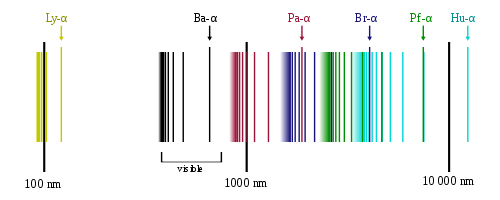
\includegraphics[width=11cm]{Preface/HydrogenSpectrum.png}
\caption{氢原子光谱}
%\label{default}
\end{center}
\end{figure}

我们发现发射光谱中原子发出的特定波长的光,在吸收光谱中也出现,只不过发射变成了吸收。

通俗地说原子就是一个爱戴戒指的人,但她只戴特定尺寸的戒指,戴腻了她就扔,扔掉戒指的尺寸和她拿来戴的尺寸完全一样。对这个现象的解释倒也简单,因为她有5个手指,每个手指粗细不同,但都有确定的尺寸。

我们有理由猜测光谱与原子的本性有关,实验也确实支持我们的这种想法,每种原子都有不同的光谱,它们的谱线出现在不同波长的位置上,就好像是指纹,人人不同,成为我们的标识。

即便是对最简单原子的光谱,比如氢原子的光谱,乍看起来都是很复杂的,但感觉它们是有规律的,或用老话讲,看起来它们是合乎比例的,只是这个比例有待我们的发现。

就好像毕达哥拉斯发现和声学里的1:2:3:4,原子物理早期的突破也来自于人们找到了一个简单、优美的数学式子,这个式子解释了氢原子光谱中可见光区域里的谱线位置(即巴尔末系):

\begin{equation}
\frac{1}{\lambda} = \frac{4}{B} \left( \frac{1}{2^2} - \frac{1}{n^2} \right)
\end{equation}

其中$n = 3, 4, ...$,这就是巴尔末公式,它解释了氢原子光谱中最显著的几条线,很快被推广为里德堡公式:

\begin{equation}
\frac{1}{\lambda} = R_H \left(  \frac{1}{n^2} - \frac{1}{n'^2}  \right)
\end{equation}

这里$n = 1,  2, ...$,$n' = n+1, n+2, ...$。

里德堡公式可以解释氢原子光谱中所有的谱线位置。

原子的稳定性仍然是很重要的问题,但现在首先要解释为什么会有谱线的规律,这个简单的公式强烈地提示我们在氢原子的问题里存在着更为简单清晰的概念体系和数学结构。

\subsubsection{玻尔理论}

%玻尔理论是导致量子力学出现的关键环节,

某种意义上说,玻尔理论从牛顿的经典力学重新退回到了毕达哥拉斯的“天球音乐”图像。天球之所以只奏响这些特定的音,是因为整体的和谐,是形的制约,使天球只能发出特定音高的音。

现在氢原子就是个小天球,它只发射(或吸收)特定波长的光,特定波长的光就是特定频率的光,频率(音)是“形”制约的结果,形的制约就是几何关系,两端固定的弦就是一维振动的形。现在我们需要发现的是氢原子的形。

首先这里有个概念需要澄清,我们说是说氢原子,但其实这里我们研究的是电子,因为质子比电子质量大太多了,质子运动的速度比电子运动的速度要小很多,或者说质子很难跟得上电子的运动,所以我们这里只需要研究电子的运动就可以了,而质子则作为固定的背景最后考虑。

现在假设有一个毕达哥拉斯的信徒来研究原子中电子的运动,他会怎么说呢?

首先电子仍然会受质子的吸引,这个力是:

\begin{equation}
F = \frac{1}{4 \pi \epsilon_0} \frac{e^2}{ r^2 }
\end{equation}

假设电子处在某个半径为$r$的正圆轨道上,电子的势能是:

\begin{equation}
V(r) = - \frac{1}{4 \pi \epsilon_0} \frac{e^2}{ r }
\end{equation}

电子的动能是:

\begin{equation}
K = \frac{1}{8 \pi \epsilon_0} \frac{e^2}{ r }
\end{equation}

电子的总能量是:

\begin{equation}
E = K + V = - \frac{1}{8 \pi \epsilon_0} \frac{e^2}{ r }
\end{equation}

电子只能在特定的轨道上运动,这就好像毕达哥拉斯派把宇宙想象为一把里拉琴,只允许在能奏响整体和谐乐音的位置上放置天球,行星在天球上沿正圆轨道呼啸而过,发出特定频率的声音,行星的速度越快,频率也越高……

现在我们只需要把这幅图像套用过来即可,电子也只能出现在特定半径的轨道上,到底是哪些半径允许,这是有标准的,类似于弦上驻波的整体和谐的标准。

%%%%%%%%%

但电子怎么能和波联系起来呢?假如要联系起来又应该怎么联系呢?

硬要往下讲就是假想的历史了。因为玻尔确实不是按这个思路思维的,而德布罗意提出物质波又在玻尔之后,受玻尔模型的启发。

我们现在要求自己有如神助,假想一个能代表电子和谐运动的波沿着电子的轨道运行,运转一圈正好是波长的整数倍,首尾相接形成圆轨道上的驻波。

\begin{equation}
2 \pi r = n \lambda
\end{equation}

我们又想到行星运转越快对应发出的声音就越高,频率$\omega = 2 \pi /T$是时间上的调制,还有波矢$k = 2 \pi / \lambda$,反映的是空间上的调制。

假如我们让电子运行的速度乘以质量(即动量)正比于波矢$k$会有什么结果呢?(纯属猜测)

假设比例因子是$\hbar$,这个比例因子是研究原子尺度物理问题必须出现的。

\begin{equation}
p = m v = \hbar k = \hbar \frac{2 \pi }{\lambda}
\end{equation}

因此:

\begin{equation*}
m v r = \hbar \frac{2 \pi r}{\lambda} = \hbar \frac{ n \lambda }{ \lambda} = n \hbar
\end{equation*}

即:

\begin{equation}
mvr = n \hbar 
\end{equation}

这就是我们猜测出的对氢原子而言,整体和谐的条件。

电子只能处在由$mvr=n \hbar$(角动量量子化条件)规定的$r$上,并满足:

\begin{equation*}
\frac{m v^2}{2} = \frac{1}{2} m \left(  \frac{ n \hbar  }{ m r }  \right)^2 = \frac{1}{8 \pi \epsilon_0 } \frac{e^2 }{r }  
\end{equation*}

求得:

\begin{equation}
r_n = n^2 \frac{4 \pi \epsilon_0 \hbar^2  }{ m e^2}, n = 1, 2, 3, ...
\end{equation}

定义玻尔半径$a_0$为:

\begin{equation}
a_0 = \frac{4 \pi \epsilon_0 \hbar^2  }{ m e^2}
\end{equation}

$r_n = n^2 a_0$(代入物理常数,可计算得$a_0 = 0.529 \times 10^{-10} m$),由这一系列$r_n$,我们可以得到一系列的能量$E_n$:

\begin{equation}
E_n = - \frac{m e^4 }{ 32 \pi^2 \epsilon_0^2 \hbar^2 } \cdot {\frac{1}{n^2}}
\end{equation}

或代入具体数值:

\begin{equation}
E_n = \frac{-13.6 eV}{n^2}
\end{equation}

因为整体和谐条件的限制,电子只能占据那一系列轨道$r_n$,因此能量的取值也是一系列分立的取值$E_n$,这一系列分立取值的电子能量就叫做能级。电子离质子越近(n小),电子的能量越低,反之电子离质子越远(n大),电子的能量就越高。

氢原子里只有一个电子,假设这一个电子处在比较高能量的轨道上,它可以向下跃迁,电子的能量将降低,多余的能量将以光子的形式释放出去,假设较高能级用$n'$标记,较低能级用$n$标记,能量差为:

\begin{equation}
h \nu = \frac{hc}{\lambda} = E_{n'} - E_n = 13.6 \times \left( \frac{1}{n^2}  - \frac{1}{n'^2} \right) eV 
\end{equation}

于是我们得到里德堡公式。

\begin{equation}
\frac{1}{\lambda } = \frac{13.6 eV}{hc} \times \left( \frac{1}{n^2}  - \frac{1}{n'^2} \right)
\end{equation}

原子的稳定性还是问题吗?在整体和谐的观念下其实已经没有问题了。我们急需澄清的是那个与电子的运动状态相联系的波到底是什么?此刻——玻尔模型的出现——说明替代范式已经出现,与其苦苦执着于老范式,不如发展新范式,而在新范式下,很多老问题是没有意义的,它们被更急迫的问题所替代。

\subsection*{练习}

\begin{enumerate}
\item 

考虑一个平面版的开普勒“圆环套圆环模型”,最内层是个圆轨道,比如水星,然后在外面套一个正方形,使正方形的四条边与水星轨道相切,然后再在正方形的外面再外接一个圆,作为金星的轨道。我们在金星的轨道外做一个正三角形,使正三角形的三条边与金星的轨道相切,最后在金星的轨道外面做一个外接圆,是地球的轨道。

现在我们可以求出水星轨道、金星轨道和地球轨道的比值了,并与观测数据进行比较。

\item

下表罗列了开普勒时代六大行星的轨道和周期,你能否把六大行星的轨道比表示为简单整数比,并计算这么做的误差是多少。

\begin{table}[htdp]
\caption{六大行星的轨道和周期}
\begin{center}
\begin{tabular}{|c|c|c|}
\hline
行星 & R (AU) & T (Year) \\
\hline
水星 & 0.387 & 0.24  \\
金星 & 0.723 & 0.615 \\
地球 & 1.0 & 1.0 \\
火星 & 1.524 & 1.88 \\
木星 & 5.2 & 11.86 \\
土星 & 9.539 & 29.46 \\
\hline
\end{tabular}
\end{center}
\label{default}
\end{table}%

\item

下图是古希腊时期的音阶图,包含两个八度和一个四度,试计算出各个频率比。同时我们也发现某些音是无法根据毕达哥拉斯的“1:2:3:4”规律计算的。这构成了音乐理论中的一个问题,即如何把剩下音的规律用数字表达出来。

\begin{figure}[htbp]
\begin{center}
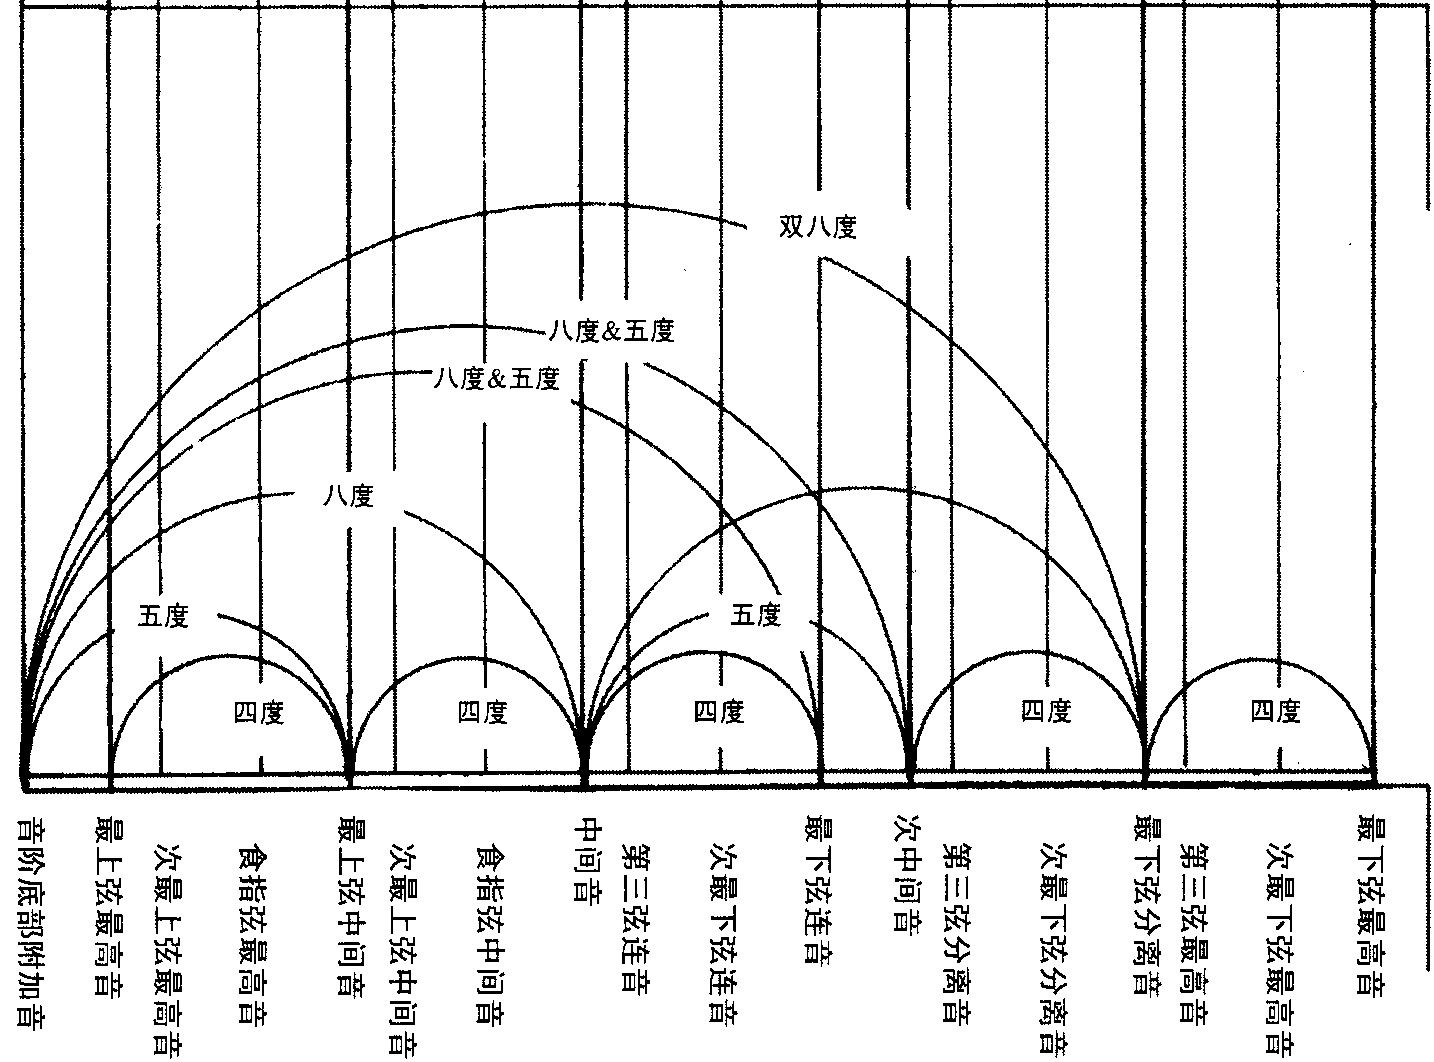
\includegraphics[width=10cm]{Preface/manyoctaves.png}
\caption{和声的基本原理:音阶。(维特鲁威,《建筑十书》,北京大学出版社,2012。图81)}
%\label{default}
\end{center}
\end{figure}


\end{enumerate}


\newpage

\section{波动和粒子}

我们给自己设定一个任务,就是努力把事情说清楚,把事情说清楚就是使听众认同,如果没有听众就是使假想的听众——另一个自己——认同。这听起来有点分裂,但确实要求这另一个自己有一点“较真”和“不断置疑”的精神。

说服,或者使用图像,或者使用语言。而使用图像更有说服力。

图像就是图景,是Picture,但要让它动起来,这需要一点想象力。有时候我们会说动起来的图像比静止的图像更真实,这是由于人在大多数情况已经适应了动起来的图像,或赋予动起来的图像以更高的审美价值。

比如拍照,我们在任一瞬间拍下的照片都是“真实”的,但拿来看却往往惹人笑,表情的瞬间也许很丑,我们从来都没有看过小于$0.01$秒的瞬间,我们看的是“时间”的绵延,是处理过的富于动感的图像,我们是借助动感的图像建立起我们的审美,对人神情的,人动态的……审美。我们觉得眨眼很迷人,但我们觉得眼睛完全闭合的瞬间丑死了。

\begin{figure}[htbp]
\begin{center}
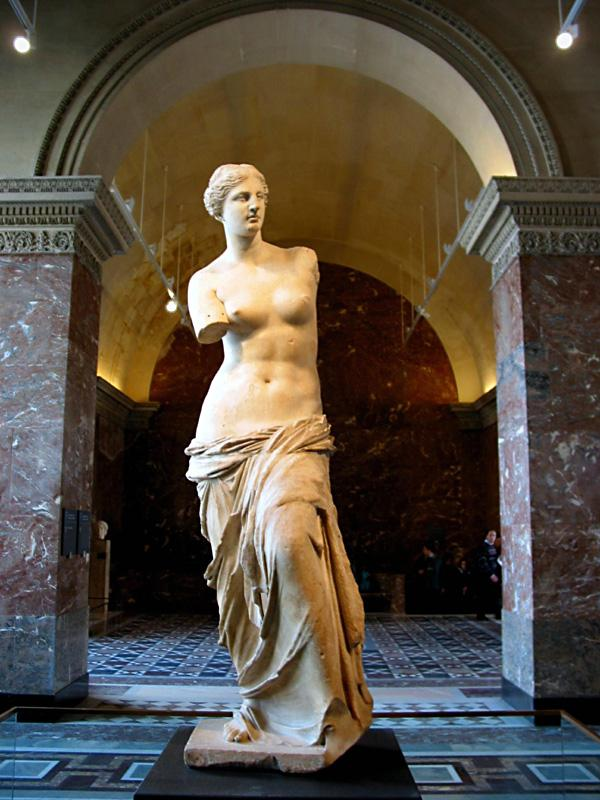
\includegraphics[width=9cm]{Duality/venus_de_milo.jpg}
\caption{米洛的维纳斯像:看起来有动感的雕像都有不符合解剖学比例的地方。}
%\label{default}
\end{center}
\end{figure}

在我们的想象中要让比如一个点动起来,一个三角形变大,旋转……是需要想象力的,而我们确实有这样的能力,有时我们在瞬间看到万丈光芒,极度具有结构特征的几何图形,色彩的斑驳变化,伴随着节奏、音乐的节奏,或我们思绪的内在节奏,在自己的脑海里轮番更替。

在这样的瞬间我们仿佛透彻了宇宙间所有的真理,但却没有合适的语言把它们描述下来,我们只能试一试,努力凭记忆把它们画下来,借着篝火,用颜料涂抹在山洞的顶上。

一些极富想象力的抽象作品。

据说这种抽象风格的绘画和极度写实的绘画同时出现。“写实”是对“可见”事物的模仿,而“抽象”是对“可以想见”事物的模仿。它们都是有力量的存在。

今天的人会设想,也许是出于交流或记录的目的,我们的祖先才开始绘画。但也有人说最早的绘画应该没有任何教育或交流的目的,它纯粹是出于精神的需要,是人灵性的发泄,是与神亲近的方式,所以它们才被创作于黑黢黢的山洞里面。

\begin{figure}[htbp]
\begin{center}
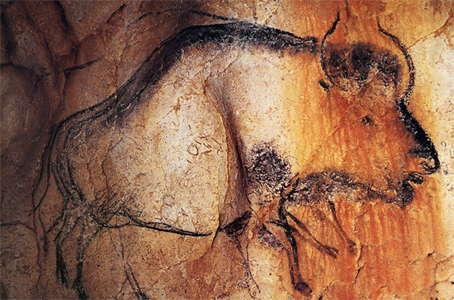
\includegraphics[width=8cm]{Duality/runningbisons.jpg}
\caption{肖维岩洞(Chauvet Cave)中的绘画已经有三万多年的历史了,几乎与人类本身的历史一样悠久,图中奔跑的野牛被表现为有很多条腿的野牛。}
%\label{default}
\end{center}
\end{figure}



\subsection{粒子的图像}

我们现在就需要通过想象而非观瞧来建立关于粒子的图像,和关于波动的图像。这是我们谈论波粒二象性的前提。

何谓粒子?

它是一个点,理想的点,只有方位,而无部分。在我的想象里它居于一个三维的空间,我可以让它上下稍微动一动,而完全不会影响其在左右方向上的位置,也不会影响其在前后方向上的位置。

假如世界只有这一个粒子,这是多么的空洞。

它可以任意地上下、左右、前后地改变位置,但对我来说是完全一样的。它都在我想象的空洞空间的中央,位置的改变无从说起。

我们必须有个参照,有了参照,我们就能说出粒子的位置了。

这个参照就是三把想象的尺子,它们互相垂直构成一个参照。或我们需要第二个点,作为原点,粒子是参照原点运动变化的。我们还需要三个箭头,标明三维空间的三个方向。

但“三”,为什么是“三”呢?

这是我们对我们所在空间的合理分类。

分类是理性的活动,是智慧的活动,谁善于分类谁就是聪明人!

“亚当证明自己是世界上第一位且最伟大的哲学家:他能根据物种的真正的本质和差异恰如其分地对它们加以区分。”

合理分类的标准是:既不重复,也不遗漏。

把我们所在的空间分解为三个不同方向是既不重复也不遗漏的。

我们也可以设想二维或一维的世界,这或者是出于限制,比如我们人类的活动就长期被限制在二维的空间上,当然是在球面上。物理学家现在也喜欢谈量子限制效应(quantum confinement effect),所谓限制就是出于某种原因,粒子(比如电子)就仅仅在二维或一维空间里运动。

想象低维空间的好处是想起来比较容易。比如落体运动,其实就是粒子在引力的作用下以越来越快的速度下落,描述这个运动只需要想象一维空间。比如炮弹的运动,就是粒子一方面以初始速度往斜刺里飞,要想飞的最远就需要以$45^o$的角度往斜刺里飞,另一方面粒子仍然受引力的作用在以越来越快的速度往地面落。

所以这是一个想象中的两个运动的叠加,先往斜刺里飞一段,再往下掉一段,然后再往斜刺里飞一段,然后再以更大速度往下掉一段。最后在我们的想象中再让这一段段锯齿缩小,让它看起来圆顺光滑一些,这就是炮弹的运动——抛物线了。

我们还可以想象很多,比如坐过山车,呼啸而下,越来越快,心悸的感觉,然后在极度的空虚中,我们向上,越来越高,在最高处,时间仿佛停止了,其实是此时速度最小,最后向下,加速,新的循环开始。

这里的窍门,是把我们自己想象成粒子,把自己的心替换为粒子的心,让我们进入粒子的世界。我们会感到有风迎面吹来,感到阻力,……

阻力是阻碍粒子运动的。我们喜欢引力,只要速度合适我们能围绕一个引力的中心(比如地球)循环往复地运动起来,一个椭圆:当我们如过山车一般冲向地球的时候,我们的速度最快,因为速度,我们从离地球最近的地方呼啸而过,然后摆脱地球,离它越来越远,向上,弯曲着向上,依靠惯性,或依靠动能($K = \frac{mv^2}{2}$)反抗地球的吸引,直到冲到离地球最远的地方,空虚地失去了太多动能,然后引力又占了上风,拉着我们加速下降,如此循环。

我们在飞,我们努力想控制飞行的轨迹,但很可惜,我们没有办法,就像梦境中的人想努力控制自己的飞行一样,徒劳和无能为力,我们在虚空中飞行,引力是唯一的外部原因,它严格地按$F = \frac{G M m}{r^2}$行为,椭圆轨道由我们的初始冲动决定,即我们在距离地球多远的地方,决定以一个什么样的速度,什么样的角度,开始运动。

(对一个二阶常微分方程$F = m a$来说,只要给定两个初始条件,初始的位置$x_0$和初始的动量$p_0$,粒子的运动就完全决定了。换句话说我们就能求解出粒子运动的轨迹。)

粒子是我们现在思维的基本单元,每个粒子都可以用质量,位置,和动量来描述。

质量就是粒子的质量。我们假设万事万物都有质量,但光子(光的粒子)除外,我们暂时先不讨论它。位置就是一个三维矢量,我们一般把它记为$\vec r$,它分解为三个固定方向上向量的叠加:

\begin{equation}
\vec r = \vec i x + \vec j y + \vec k z
\end{equation}

动量的定义是质量乘以速度,速度定义为对位置的微分:

\begin{eqnarray}
\vec v & = & \frac{d \vec r}{d t} \\
\vec p  & = & m \vec v
\end{eqnarray}

位置,速度,动量都是矢量,还有力,这给我们的想象力带来极大的挑战,为了思维的轻松,我们往往把它们想象为二维的或一维的。

粒子在三维空间里飞来飞去,但它并没有自由意志,它是由力和它的初始状态完全决定的,我们可以把粒子位置随时间变化的关系求出来。

\begin{equation*}
 \vec r(t)
\end{equation*}

粒子如$\vec r(t)$般在时间和空间里存在,$\vec r(t)$就是粒子的世界,粒子的一生,它完全由它受到的力,它的初始位置和它的动量决定。这是很宿命的世界。

如果只存在牛顿力学,我们的世界就是这样的一个世界。万事万物不过是粒子的集合,很多很多个粒子,虽然多,但它总数的过来,比如整个宇宙中质子的数目就是$10^{80}$数量级。

只要可数,我们就可对它们列方程:可数个质点,可数个力,可数个初始位置,可数个初始动量,一个非常巨大,但确实是可数个微分方程联立,虽然我们不可能对这$10^{80}$个方程求解,但它们的解是存在的,我们求不出是因为我们人自身的局限。

如此巨大的方程,在我想象的世界里是即刻被求解出来的,$10^{80}$数量级的粒子,它们冲撞,互相缠绕,各自远离,经过无限时间后又相互吸引,重新凝聚……就如一场戏剧在笛卡尔空间这个三维的舞台上出演。

每个粒子都是莎士比亚戏剧中的一个人物,各有各的命运,但这一切在戏剧开演的一瞬就已经决定,我们张大嘴巴好奇地看,假想自己进入到戏剧里,与某个粒子化为一体,或进入环绕某个粒子运行的轨道,我们有我们的自由意志,但我们就如梦境中的人一样,我们根本就无法驾驭粒子的运动,我们徒劳地想,徒劳地扭动思想的身躯,但这场戏只由力,初始位置和动量决定,我们的命运早已被安排,只是我们不知道。而我们所有的意志都是无用的,我们不受我们自己指挥。

\begin{figure}[htbp]
\begin{center}
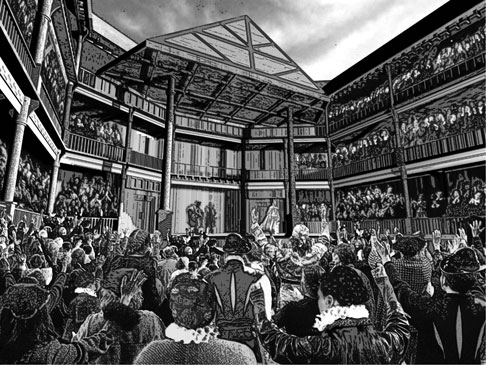
\includegraphics[width=8cm]{Duality/ShakespeareanTheater.jpg}
\caption{莎士比亚时期的舞台提供给我们想象空间和运动的原型。}
%\label{default}
\end{center}
\end{figure}

所谓粒子的图像就是粒子们在虚空中运动,它们各有各的质量,相互之间存在着万有引力。假如上帝是造物者的话,他在造物的瞬间会用他的大手抛洒出这$10^{80}$数量级的粒子,然后以他的全能使其按各自的方式具有初始位置和初始动量,然后他老人家就休息了,在异度空间翘着脚看质点们成形(pattern formation)演化。

这里虚空很重要,无虚空粒子就没有舞台。而所谓质点则是一些没有大小、形状的几何点,它们可以集中地携带一份能量和一份动量。虚空是古代原子论强调的,但他们认为原子有形状,因为古代原子论者没有发现相互作用(力),它们需要形状来解释物性。

古代原子论者还会强调有粒子的突转(swerve),这是想给它们灰暗的世界图景保留一点人性的努力,突转后来被看做是“自由意志”的体现,被挪用到基督教哲学中。引入突转纯粹是哲学的考虑或审美的原因,这在僵硬或被构建得很死的牛顿力学里是没有地位的。粒子有没有自由意志,会不会突然神经质似的蹦跶一下是微分方程($F = ma$)决定的,它告诉我们不行,就是不行!

牛顿力学关于世界的图景是缺乏解释力的,它归根到底只是一个关于机械运动的理论。原则上说由此出发可以构建一个物性的理论,甚至一个电磁学的理论,但实际上太不可行了以至于几乎没人尝试。

\subsection{波动的图像}

牛顿本人也研究光学,它认为光是由很多细小,运动速度很快的粒子组成的,这其实就是在延续古代原子论者的观点。光的粒子说可以解释光的直线传播,光的反射、折射,光可以被物体遮挡等常见的光学现象。

牛顿的粒子说是很不完备的,仅可看作是为了理解方便而做的一种权宜性假设,比如他并没有告诉我们光的粒子(光子)的质量是多少?它的能量是多少?它的动量又是多少?以及如何由这些基本的物理陈述出发,解释牛顿环的条纹间距。

仅仅说光子砸在玻璃上然后激起涟漪形成了圆环是很有想象力的猜测,但还不构成一个靠谱的理论。

一个靠谱的光学理论必须能够对最突出的光学现象做出定量的解释。就好像我们在氢原子的玻尔理论中体会到的,一个靠谱的关于原子的理论首先要能定量地解释这个领域里最独特而且也是最显著的现象,比如——里德堡公式。

\subsubsection{三棱镜分光实验}

波动图像的兴起和牛顿粒子图像在光学研究中的无能为力有关。但吊诡的是牛顿同时还是近代光学实验的先驱,他做的那些实验恰恰可以用波动说去解释。

这里我们只讨论他的三棱镜分光实验。

\begin{figure}[htbp]
\begin{center}
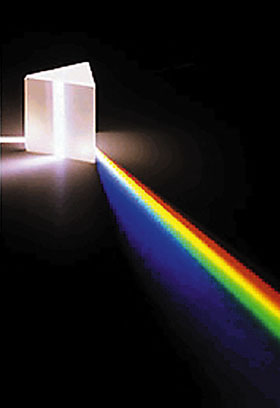
\includegraphics[width=5cm]{Duality/newtonprism.jpg}
\caption{牛顿的三棱镜实验。}
%\label{default}
\end{center}
\end{figure}

彩虹是自然界中常见的现象,又或者我们喝口水对着太阳喷一口,就可看到圆弧形的颜色分布。这些都提示我们,光,看上去很纯,但其实很复杂,也许还可以进一步分类。

牛顿就是那个对光进行分类的聪明人,他是这么做的:

在封闭的屋子里,把厚厚的窗帘稍稍拉开一条缝,使光透进来,然后拿一个玻璃做的三棱镜,玻璃的折射率比较大,它可以使光比较明显地偏离原先的运动方向。但玻璃的折射率对不同波长的光是不一样的,不同波长的光会有不同偏转的角度,不同波长对应不同颜色,一束白光于是就被分成了一系列颜色的光。

假如我们只留下一种颜色,把其他颜色挡掉,继续让光通过三棱镜,我们发现光不会再继续分解了。

在我们的视觉经验里,自然光或白光是纯净的,但现在白光是复杂的,可以被某个操作继续分解,而带颜色的光反而有可能是纯净的了,它不能被这某个操作继续分解。

\begin{table}[htdp]
\caption{可见光的波长($nm$)}
\begin{center}
\begin{tabular}{|c|c|c|c|c|c|}
\hline
   紫 & 蓝 & 绿 & 黄 & 橙 & 红 \\
   380-450 & 450-495 & 495-570 & 570-590 & 590-620 & 620-750 \\
  \hline
\end{tabular}
\end{center}
%\label{default}
\end{table}%

初看起来这有点象变戏法,但为什么我们相信科学家(但不相信魔术师)呢?

原因是科学家不隐瞒自己的发现,科学家做演示(实验其实就是一种“公开”的演示),但他会把演示的步骤一步一步告诉你,使大家都能重复。这个说法在今天有点不确切,但主要是因为科学已经发展到极其复杂和昂贵的程度,致使普通人很难重复他们的工作,但在科学家社群内,各个竞争的小组还是可以的,否则科学发现就不会得到确认,科学活动的功利价值——通过首先发现权获取名誉和利益——就无从体现。

而魔术师就不一样了,他也表演,但他不会教你,除非你付钱成为他的徒弟。

科学活动有一套规范能够认定牛顿并非是在变戏法晃点大家,否则这么反常识的结论大家是不会承认的。而今天我们讨论科学的时候也一定要记住,科学之所以可信,并不在科学方法的严谨,也不在科学家多么有良心,而全在有一套科学实作之成规,我们信赖的是制度,而非个人或具体的科学知识。但普通人在谈论科学话题的时候往往因为知识上的欠缺,就先自己矮了一头,这是不对的,我们当然需要一定的知识做基础,但我们考虑问题的焦点应该是拷问科学实作的成规,检讨其在运作中的漏洞等等。

(这里面的道理其实很简单,假想你是个总统,你需要做决策,很多方面的决策,并对这些决策负责,但显然你不可能是每一方面的专家。)

\subsubsection{水波}

牛顿关于光学的系列实验开创了物理光学,而牛顿粒子说的无所作为则给了波动说机会。

波动也是我们日常生活中常见的图像,比如:水波。

假设我们身处一个巨大的游泳池,或者有人造的海浪或者有天然的海浪(以海为池),套上游泳圈,我们会随着波浪周期性地一起一伏,这是很好玩的体验,起来到顶是波峰,而降到低是波谷,在波峰的时候,我们会看见远处某段距离外的波峰向我们移来,当我们降到谷底的时候,我们会感到波峰离我们越来越迫近,像座小山一样扑来,然后我们随着这下一个波峰的到来和救生圈一起飞快的上升,很像坐过山车,到了波峰的顶部会有空虚的感觉,然后又加速向下,如此反复。

没有水面我们就体验不到这美妙的运动,在每个波峰来临的时候,我们都感到它巨大的力量,它狠狠地把我们从谷底掀起来,往上扔,波峰越高,我们越体验到它巨大的力量。我们无时不刻、处处体验到波的能量,当我们冲到波峰的顶部的时候我们有很大的势能,势就是“位置的优越”,因为我居于此位置,我可以把这位置的好处转化为运动的动能去冲,而当我们居于波谷的时候,我们其实是处于另一个波峰,因为水波的弯曲,水波整体的挤压,我们仍然会居“位置的优越”,或换句话说,我们仍有一个大的势能……

波的能量正比于振幅的平方($\propto A^2$),水波的能量分布在整个水面,波传播到哪里,波的能量就到哪里,我们套上救生圈就可以体验到这种能量。

波是整体的运动,当我们研究水波的时候,能量并非集中在某一点,它是能量的分布,“均匀”地分布在整个波动着的水面。此时虚空的概念就多余了,空荡荡的舞台可以让莎士比亚戏剧中的人物一个个登场,但水波必须要有个游泳池,里面装满水,水波存在于水波的表面上。

在水面上,每一点都随着水波在波动,我们如果一个一个位置地去描述水波的运动可要累死了,因为位置是不可数的(innumerable),我们没有办法用$1, 2, 3, ...$的方式遍历水面上的每一个位置。这是和我们研究牛顿粒子世界的一大区别,在那个世界里,有$10^{80}$数量级个粒子,虽然很多,但到底可数,可以用$1, 2, 3, ...$的方式穷尽。

这里我们必须说$1, 2, 3, ...$的方式其实是个很强大的方式,如果你不限定时间的话,我们可以穷尽无穷多个粒子。这个无穷有专门的名字,叫:“阿列夫零”,即最低阶的无穷多,或可数的无穷多,即用$1,2,3...$数数的方式可以穷尽的无穷多。

\subsubsection{无穷多的自由度}

由此我们已经进入了场论的研究领域,所谓场论就是研究无穷多自由度的运动。场就是物理量随时间、空间的分布,比如电场$E(x,t)$,空间上的每个点$x$都有自己的场,不同位置的场如$E(x_1)$和$E(x_2)$的取值是独立的。

$E(x_1)$和$E(x_2)$是独立的自由度,或每个不同的$x$对应的$E(x)$都是一个独立的自由度,考虑到在空间里有无穷多个$x$,我们这里就有无穷多的自由度。

(自由度就是描述一个物理系统所需要的独立变量的个数,比如对自由落体,只需要一个,即位置。)

假设我们讨论一个经典的场论。我们应如何研究波动呢?

一种方法是把它离散化,因为处处皆在的连续太难想象了。我把它们想象成为一个弹簧床垫,在场里面做想象的切割,每一个小方块,或每一个三角形,六角形,收缩成为一个质点,每个质点的质量将等于面积乘以密度,然后我在想象中让每一个质点按照某种结构相连,用假想的弹簧相连,如果你不想让你的场破碎的话,你就必须用弹簧把它们编织起来。

此时上帝变成了一个编织弹簧床垫的工人,弹簧各有各的弹性系数,它们可用弹性模量来表示。离散模型的好处是好想。一个离散的模型又部分地回到了粒子的图像,但粒子是被固定在各自平衡位置附近的,它们被弹簧束缚住,不能自由地在虚空中跑来跑去。

波的能量现在体现为所有质点的能量和,而每一个质点又由动能和势能两部分组成,很多细小的$\frac{1}{2} m v^2$和$\frac{1}{2}k x^2$之和,然后利用密度,弹性模量等概念再重新把这些关系表示为连续的情形。这时我们会得到一个用连续的场$\varphi(x,t)$表示的动能和势能。

我们使用一套由牛顿力学发展出的技巧(相当于是某种数学变换),我们不考虑力,转而考虑拉氏量$L = T - V$,它的定义是动能减去势能,由拉氏量出发我们利用一个变分求极值条件,就可以得到波动方程。波动方程和我们利用偏微分方程技巧求得的形式是相同的。它的解却可以是自由的,即波可以在弹簧床垫里自由地传播,并不衰减。

这是一个很漂亮的结果,如果你把“弹簧床垫”看做是个粒子的世界的话,这里的粒子是“固定”不动的,它们只能在各自位置的附近做微小的振动,但这些振动由于弹簧的耦合,却可把一个局部的振动向各个方向传播出去,传播给其他位置上的粒子。整体看就是一个波动在自由地传播,所谓自由指的是波动在传播的过程中并不损失能量,而且波动确实是可以传播到弹簧床垫的任意部分的。

\subsubsection{波的干涉}

两列波相遇,会发生干涉现象。这也是我们极熟悉的自然现象。

比如在夏日的傍晚,我们来到一个池塘边,有轻风吹过水面,池塘里泛起一阵涟漪,此时追踪波的运动,观察它,假如波撞在一根芦苇上,我们会发现水波似乎以芦苇为中心形成了一个新的波,你如果仔细看,还会发现波每碰到一个细小的障碍物,都会以此为中心形成一个新的波,以同心圆的形状向外扩散。

波动运行中的每一个点都可看做是一个新的波源,而波动整体的效果就是这无数波源扰动的波动的叠加。这就是惠更斯原理。

这么说很有美感,只是具体计算的时候会很麻烦。但假如波动撞到某面墙上,我们在这墙上只开两个小孔,这个运算就会变得简单。我们只需要计算两列波的叠加,这两列波其实是源自同一个波的,是我们把它们的兄弟姐妹们都挡住了。

如前所述,波动可以看做是相位的奔跑,相位是$k x - \omega t$,假如我们考虑某一时刻波动的情况,即$t$是固定的,我们需要看的是$k x$。

现在一列波由A出发按照某个路径(Path A)跑了$x_A$距离,相位是$k x_A$,而另一列波由B出发按照某个路径(Path B)跑了$x_B$距离,相位是$k x_B$,假设这两列波最终在C相遇。

如果相位差$k (x_A - x_B)$正好是$2 \pi$的整数倍,意味着两列波是同步的,振幅会变为$2A$,而波的强度则会正比于$4A^2$。

但假如相位差$k (x_A - x_B)$正好是$\pi$的奇数倍,则意味着当一列波位于波峰时,另一列波必位于波谷,它们总是相消的,振幅会变为$0$,波的强度也只能是0了,这是无法再弱的情况了。

当然还有居于二者之间的情况,但我们不妨把最强和最弱(0)当做标志。

\begin{figure}[htbp]
\begin{center}
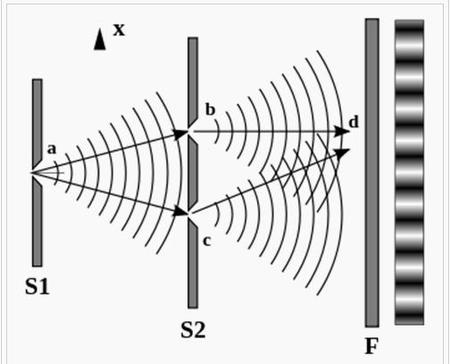
\includegraphics[width=8cm]{Duality/doubleslit.jpg}
\caption{双缝实验示意图。}
%\label{default}
\end{center}
\end{figure}


这就是著名的双缝实验,我们将会在双缝的对面观察到一系列振动“最强、最弱、最强、最弱……”的条纹分布。

对水波而言,我们是能直接看到这种现象的,所谓水波涟漪。就是这种波峰、波谷错综相杂的条纹镶嵌。

光的干涉要难些,首先对光源有要求,我们必须用特定波长的光源,而且光源要稳定,行话叫相干光;另外由于光的波长本来就很短,这需要我们专门设计实验才能观察到干涉现象。

~

光的干涉现象用波动图像很容易解释,而这仅仅是个开始,还有衍射现象,艾里斑等。衍射光栅因为对分辨不同频率/波长的光具有特别强的分辨本领成为测量光谱现象强大的工具。

物理光学就是波动光学,它很快超越几何光学成为光学研究的主流。比如我们可以用衍射光栅测量氢原子的光谱,类似地还有钠原子光谱,我们只要在炙热的火焰里放进某种元素的金属丝,我们就可以研究这种元素的光谱了。

到19世纪,光的波动说开始全面占上风。等到赫兹做实验证明电磁波也是波动,并且如光波一样有干涉、衍射等现象,物理学家普遍相信光波就是一种电磁波,光的粒子说就正式被扫进了历史的故纸堆。(就像我们现在说到以太或燃素的感觉一样)

但情况在一点点的起变化。

\subsection{黑体辐射}

19世纪末,随着工业的进步,人们开始用衍射光栅去研究黑体辐射。所谓黑体就是一个大空腔,这个空腔包纳着一个大空间,这个空间就是电磁场的海洋,各种电磁波在空腔里碰撞奔腾着,就好像是个电磁波的冲浪游乐场。空腔(把它想象为太上老君炼丹的炉子)的温度是可以调节的,电磁辐射场与空腔达成了热平衡,所谓热平衡是个与材质无关的事情,这很平等,铁的$300^o$和陶瓷的$300^o$是一样的,它们都能和$300^o$的电磁辐射场达到热平衡。

我们还记得热交换的几种途径:传导、对流和辐射。这个辐射就是电磁辐射,太阳离我们很远,中间又没有导热的介质,传导和对流都无从谈起,靠的就是辐射。所以我们说辐射、热辐射,还是电磁辐射讲的都是一个东西。

我们可以在想象中把电磁辐射场的一部分画个范围,其内是个物体,这个物体——其实就是电磁辐射场——与腔体通过辐射达成热平衡,假如腔体的温度是$T$的话,那么电磁辐射场也处在温度$T$。

现在温度进来了。

在统计物理的框架内,温度和无规则的热运动有关,无规则代表着信息的缺失,我们没法知道系统内每一个质点的运动,但我们知道它们作为整体的统计规律,这个规律说,质点具有动能$K$的几率正比于玻尔兹曼因子$e^{-\frac{K}{kT}}$。这个概念我们可以推广运用到黑体辐射中。

所谓黑体辐射就是很多电磁波的振动,很多振动的模式,它们的能量正比于电场强度的平方,也正比于磁场强度的平方,而现在电场和磁场就相当于质点的动能$K$。

我们不进入计算的细节,只是声明统计物理现在就能排上用场了,我们有很多振动的模式,每个振动模式用不同的波矢$\vec k$表示,很多波矢,每个波矢对应的振动都有能量,我们希望把这些能量都加起来,我们现在并不知道每个振动的能量,我们求热力学平均,再把它们加起来,并把能量的密度$u_T(\nu)$用波长或频率表示出来。

\begin{equation}
u_T(\nu) = \frac{ 8 \pi }{ c^3 } \nu^2 k_B T
\end{equation}

这是一个很漂亮的计算,就一个毛病,计算出来的能量密度对短波长(或高频率,所谓紫外)是发散的,即$\nu \to \infty$时,$u_T(\nu) \to \infty$。这导致了一个荒唐的结果,即每单位空间我们都有无穷多的能量在等着我们。而且理论计算出来的能量密度随波长的分布与实际实验测量的结果也不匹配。

1900年,普朗克利用内插法凑出了一个黑体辐射的能量密度公式,与实验数据符合的很好:

\begin{equation}
u_T (\nu )  = \frac{ 8 \pi h \nu^3  }{ c^3 } \cdot  \frac{1 }{ e^{ \frac{ h \nu }{ k_B T } }  - 1 }
\end{equation}

这个公式叫普朗克公式,它是凑出来的,我们还需要把它推导出来。但考虑到三维太复杂了,我们先考虑一维,然后由一维的结果推广。

首先对电磁波而言,每个波矢$k$都有两个独立的振动模式,比如一个是$x$线偏振光,另一个模式就是$y$偏振光。其次对大小为$L$的一维空间而言,电磁波存在于这样一个空间里需要满足一定的边界条件,比如在边界处某个方向的分量为0等等。这要求波矢满足这样的关系:

\begin{equation}
k L = n \pi
\end{equation}

这里$n = 1, 2, ...$,可见并不是一个$k$允许,而是一系列的$k$都满足边界条件和波动方程,所以我们考虑的空间里是很多不同波矢电磁波的叠加。

把这个结果推广到三维:

\begin{equation}
\frac{1}{8} \cdot 2 \cdot \frac{4 \pi k^3}{3} V = N \pi^3
\end{equation}

针对这个公式做一些说明:

\begin{enumerate}
\item 

因子$\frac{4 \pi k^3}{3}$对应的是波矢小于等于$k$包围起来的波矢空间的体积;

\item

因子$\frac{1}{8}$表示我们这里的求和是只针对$k_x >0, k_y > 0, k_z >0 $进行的,对应是波矢空间里的$\frac{1}{8}$体积;

\item 

因子$2$指的是对每个波矢,有两个独立的振动模式;

\item

V是电磁波所在空间的体积;

\item

$N$代表波矢小于等于$k$时系统允许的独立振动模式的个数;

\item

$\pi^3$,因为现在是三维了,波矢空间的体积乘以空间的体积对应的应该是$\pi^3$。

\end{enumerate}

黑体辐射能量密度$u_T(\nu)$是单位体积内处于频率由$\nu $到$\nu + d\nu $的电磁波的能量,当然是热力学平均意义下的能量。

现在首先要问单位体积内处于频率由$\nu $到$\nu + d\nu $的独立的电磁振荡的数目有多少,我们管它叫“态密度”(Density of states),写成数学的式子就是:

\begin{equation}
\frac{1}{V} \frac{d N (\nu)}{d \nu}
\end{equation}

首先由$\frac{1}{8} \cdot 2 \cdot \frac{4 \pi k^3}{3} V = N \pi^3$,我们可求出$N(k)$,

\begin{equation}
\frac{N(k )}{ V } = \frac{ k^3 }{3 \pi^2}
\end{equation}

然后根据$k = \frac{2 \pi }{ \lambda}  = \frac{2 \pi \nu}{c}$,把$N(k)$变换为$N(\nu )$:

\begin{equation}
\frac{N(\nu)  }{ V } = \frac{ 8 \pi }{ 3 } \frac{ \nu^3  } { c^3 }
\end{equation}

现在态密度$g (\nu)$是:

\begin{equation}
g(\nu) = \frac{1}{V} \frac{d N (\nu)}{d \nu} = \frac{8 \pi \nu^2 }{ c^3 }
\end{equation}

现在黑体辐射的能量密度可表示为:

\begin{equation}
u_T (\nu) = g (\nu) \left\langle \epsilon (\nu)  \right\rangle_T
\end{equation}

这里$\left\langle \epsilon (\nu)  \right\rangle_T$表示对振荡频率为$\nu$的电磁波能量的热力学平均。

如果使用经典的统计物理,我们需要做的就是对电磁波的能量$ \frac{\epsilon_0}{2} E^2 + \frac{1}{2 \mu_0} B^2 $进行热力学平均,计算结果为$k_B T$,于是我们得到了先前的那个会发生紫外发散的能量密度。

\begin{equation}
u_T(\nu) = \frac{ 8 \pi }{ c^3 } \nu^2 k_B T
\end{equation}

这个公式最早是由瑞利和金斯计算出来的,因此也叫瑞利-金斯公式。

~

普朗克面对的就是这样一个问题。他并没有直接假设电磁波本身是量子化的,他假设的是电磁波与物质发生能量交换时,必须以一份一份的方式进行,一份就是一个量子(quanta),大小是:

\begin{equation*}
h \nu
\end{equation*}

这里$h = 6.626 \times 10^{-34 }$焦耳·秒,叫做普朗克常数。现在频率为$\nu$的电磁波按普朗克的假设就是它可以用$n = 0 , 1, 2, ...$的整数份额与物质交换能量。

而以我们现在的观念则说电磁辐射本身是量子化的,对频率为$\nu$的振荡模式,它可能存在1个激发,也可能是2个激发……,当然也可以是0个激发,对应的就是没有一个$h \nu$光子的状态。

现在我们可以按照统计物理的基本法则计算$\left\langle \epsilon (\nu)  \right\rangle_T$:

\begin{eqnarray*}
\left\langle \epsilon (\nu)  \right\rangle_T &=& \frac{ \sum\limits_{n=0}^{\infty} n h \nu e^{- \beta n h \nu } }{ \sum\limits_{n=0}^{\infty} e^{- \beta n h \nu  } } =  - \frac{\partial }{\partial \beta } \ln \sum\limits_0^{\infty} e^{-\beta n h \nu } \\
{} &=& - \frac{\partial }{\partial \beta } \ln \frac{1}{ 1- e^{- \beta h \nu} } = \frac{\partial }{\partial \beta} \ln \left( 1 - e^{- \beta h \nu} \right)
\end{eqnarray*}

这里$\beta = \frac{1}{k_B T}$,所以:

\begin{equation*}
\left\langle \epsilon (\nu)  \right\rangle_T = \frac{ h \nu e^{- \beta h \nu } }{1 - e^{ - \beta h \nu }} = \frac{ h \nu  }{e^{\beta h \nu} - 1 }
\end{equation*}

最终我们得到了普朗克公式:

\begin{equation}
u_T (\nu )  = \frac{ 8 \pi h \nu^3  }{ c^3 } \cdot  \frac{1 }{ e^{ \frac{ h \nu }{ k_B T } }  - 1 }
\end{equation}

在黑体辐射实验之前光的波动说可谓是牢固地竖立起来了,但普朗克的量子假说打开了一个缺口,这之后的光电效应、康普顿散射等实验都更进一步说明光在这些实验里必须被理解为粒子才可以获得一种简单的解释。

\subsubsection{维恩位移定律}

热辐射即固体、液体或气体由于自身温度($T$)而释放的辐射。用三棱镜使热辐射折射,不同波长的光会被三棱镜折射到不同的方向上,测量不同方向上的光强分布,我们得到连续谱,即一个强度随波长连续变化的分布。

温度低于500摄氏度时,大部分热辐射能量在红外波长的区域。随着温度的升高,辐射能量的主要部分逐渐向短波高频端移动,移动到可见光,紫外光等等。

\begin{figure}[htbp]
\begin{center}
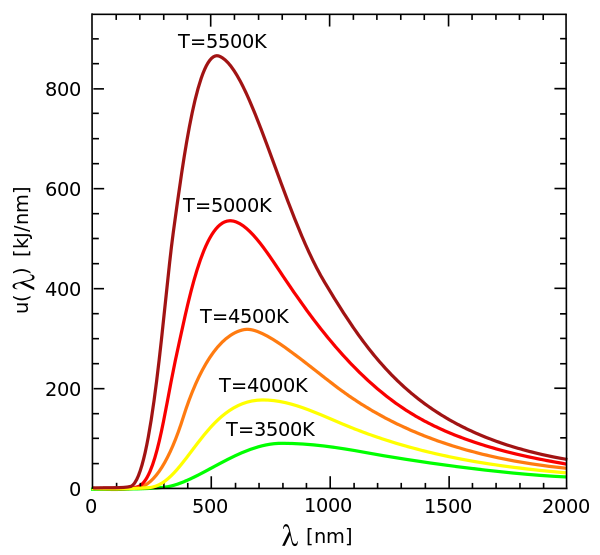
\includegraphics[width=10cm]{Duality/Wiens_law.png}
\caption{维恩位移定律。}
%\label{default}
\end{center}
\end{figure}

看来热辐射的主要部分的波长和温度是成反比的,这就是维恩位移定律(Wien's displacement law):

\begin{center}
$\lambda_{max} T = 2.898 \times 10^{-3 }$米·开尔文
\end{center}

这里$\lambda_{max}$是使谱分布$u_T(\lambda)$取最大值的波长。

这个现象本身是很常见的,比如我们在看电影《大闹天宫》的时候,太上老君把孙悟空扔进炼丹炉里烧,炼丹炉除一个开口外都是封闭的,而那个开口就是黑体,随着炉子里面的温度逐渐升高,窗口会显现不同的颜色,按照波长由长到短,或频率由低到高的次序依次出现,“红橙黄绿青蓝紫”。

用这个方法我们可以确定远方恒星的温度,比如一颗黄星的表面温度就比一颗红星的表面温度高。

\subsubsection{斯特番-玻尔兹曼定律}

物体的温度越高,发射的总能量就越多,这就是斯特番-玻尔兹曼定律(Stefan and Boltzman's law):

\begin{equation}
R(T) = \sigma T^4
\end{equation}

这里$R(T)$是辐射本领,被定义为单位表面积物体向外辐射出的功率。

\begin{equation}
\sigma = 5.67 \times 10^{-8} J s^{-1} m^{-2} K^{-4}
\end{equation}

叫做斯特番-玻尔兹曼常数。

~

我们现在可以来做一个练习:

假设太阳、地球、火星、金星都可看作是绝对黑体,利用斯特藩-玻尔兹曼定律,估算金星、地球和火星的表面温度,这给出了一个讨论温室效应的定量框架。

太阳半径: $R_S  = 6.96 \times 10^5 km$

太阳表面温度: $T_S  = 5780K$

水星距离太阳的距离是0.39AU,火星距离太阳的距离是1.52AU (1AU就是地球到太阳的距离,$1AU = 1.496 \times 10^8 km$)

根据斯特番-玻尔兹曼定律,太阳的总辐射功率为:

\begin{equation*}
P = \sigma T^4 4 \pi R_S^2
\end{equation*}

其中只有一部分会照在“地球”, 比例是: 

\begin{equation*}
\frac{\pi R_E^2}{4 \pi D^2}= \frac{R_E^2}{4 D^2}
\end{equation*}

这里$D$是地球到太阳的距离(地心到日心)。

假设地球表面温度是$T_E$,地球向外辐射的功率是: 

\begin{equation*}
\sigma T_E^4 4 \pi R_E^2
\end{equation*}

当这个辐射功率和吸收功率相等时,可估算出地球表面的温度。

\begin{equation*}
\sigma T^4 4 \pi R_S^2 \cdot \frac{R_E^2}{4 D^2} = \sigma T_E^4 4 \pi R_E^2
\end{equation*}

解出:

\begin{equation*}
T_E = T \sqrt{\frac{R_S}{2D}} = 278.77 K
\end{equation*}

这个温度与地球半径($R_E$)无关。更多结果见下表:

\begin{center}
\begin{tabular}{|l|l|l|l|l|}
  \hline
  % after \\: \hline or \cline{col1-col2} \cline{col3-col4} ...
  {} & 水星 & 金星 & 地球 & 火星 \\
  距离(AU) & 0.39 & 0.73 & 1 & 1.52 \\
  温度(K) & 446 & 326 & 279 & 226 \\
  温度(${}^oC$) & 173 & 53 & 6 & -47 \\
  \hline
\end{tabular}
\end{center}

碳基生命是发生在液态水的环境里的,而水在$0 - 100 {}^o C$保持液态,我们验证了地球确实是太阳系里最适合生命存在的星球。

%%
~

我们现在已经基本明了粒子的图像与波动的图像了。

那它们为啥不兼容呢?

从概念的角度,二者都是理想的模型,粒子要求“点”,能量和动量都被集中地携带,在虚空中穿行。而波动是运动的整体状态,需要一个介质,或像电磁波那样,电磁场本身就是实实在在的物理量,它们在时空中有个分布,波动作为一种整体的运动,能量正比于振幅的平方,充满并且连续地分布在整个介质或场里面。

场的概念比介质的概念更根本,经典物理里强调介质,无非是给出了一种使“场”得以现身的结构,一旦我们写出了场的拉氏量,场就已经数学化了,有了描述场的数学式子,我们要介质何用呢?

对电磁场的研究,我们是先得到场的陈述的,但历史上物理学家对这一数学陈述并不满意,他们试图找出电磁场的介质——以太——其实就是想构造出一种使电磁场得以呈现的机械模型。但电磁场太复杂了,物理学家们一直没成功。到了20世纪,物理学家很快就被接踵而来的新问题吸引,忙别的事情去了。

有一种克服危机的方法就是制造出更紧迫的危机,使矛盾在更高水平和更激烈的程度上爆发,具体到这里,寻找以太导致了相对论的发现,而相对论一旦被大家接受,寻找以太这个任务就不存在了。

\subsection{像波一样的粒子}

我们把Duality翻译成“二像性”,所谓像就是“like”,最有名的二像就是“波粒二像性”,字面的意思就是既像粒子又像波,或有时候像粒子有时候像波。

粒子和波如前所述是两幅图像。所谓像波,就是“wave like”,像粒子,就是“particle like”,这是个构词的游戏,我们可以说“wave like particle”,“像波一样的粒子”,或“particle like wave”,“像粒子一样的波”。

\subsubsection{电子的发现}

在历史上“波动”和“粒子”是两个相互竞争的图像,比如19世纪末,标准的科学问题是“阴极射线是一种粒子还是一种波动?”

在这类争论中,科学家们就像是在搞选举,分裂为两个阵营,以对阴极射线的争论为例,大多数德国科学家认为阴极射线是波动,而大多数英国科学家则认为阴极射线是粒子。

双方都拼命找有利于自己的证据,比如有人用集电器(法拉第笼)收集阴极射线,发现阴极射线是带负电的,由此猜测阴极射线是一种带负电的微小粒子(电的“原子”)。

对立的阵营于是就给阴极射线管加上磁场,然后论证说如果阴极射线是个粒子的话,那它应该在磁场中发生偏转,但阴极射线却没有偏转。这是波动说给粒子说的一个强有力的阻击,但显然没发生波普尔所说的证伪。

这里存在着一个问题,即实验也是可以改进的,否定性结论也和实验的方案、实验的精度有关。比如阴极射线在磁场中是应该发生偏转的,但由于实验条件的限制,比如真空度,比如磁场的绝对强度等等,德国科学家就是没有发现阴极射线能够在磁场中发生偏转。可以想象德国科学家做出了这个否定性结果很Happy,因为缺乏对粒子说的信仰,他们没有进一步改进实验的动力。

回到当时的历史情境,主张波动说意味着你必须把阴极射线看做是某种符合电磁辐射方程的电磁场,你能够通过计算解释实验中的主要现象,又或者你能够证明把阴极射线看做是一种带电粒子,将完全不能解释实验现象,或将导致与实验相反的结论。

电磁波还是带电粒子?这意味着两套方程,两种数学操作的手续,它们吃进一些数据,然后再吐出一些数据,吃进的数据是由实验来的,而吐出的数据也是要和实验比照的。如果我们采用了一套手续,就意味着我没法同时采用另一套手续。

我们讲“波动和粒子是两幅不相容的图像”,我们的意思是:它们是互相竞争、互相替代的两种理论近似(Approach)。而这两种近似又确实是以“波”和“粒子”两种图像为核心构建的。

所谓波就是充盈于整个空间的某种(物理)量的分布,比如电场和磁场,我们可以直接测空间中电场和磁场的强度,电场和磁场的强度又对应能量,因为电磁场是充盈于整个空间的,我们可以在想象中划定一块体积,能量正比于体积,单位体积电磁场的能量就是电磁场的能量密度:

\begin{equation}
\rho(\omega) = \frac{\epsilon_0 E^2(\omega)}{2} + \frac{B^2(\omega)}{2 \mu_0}
\end{equation}

这里我们把电磁场的能量密度$\rho(\omega) $表示为和频率($\omega$)有关的形式,我们在想象中对电磁场进行分类,按照不同振动的频率分类,然后再把它们加起来。

所谓粒子,就是集中地携带一份动量和能量,假如不考虑相对论的话,能量可以写为:$T + V$,动量可以写为:$p = mv$。粒子的运动满足牛顿方程。

比如带电粒子在磁场中运动,它会受到洛伦兹力$F$的影响,洛伦兹力的大小是$q v B$,这里$q$是带电粒子携带的电量,$v$是带电粒子运动的速度,$B$是磁场强度。洛伦兹力与带电粒子运动的方向垂直,如果粒子带正电的话,粒子速度$\vec v$,磁场$\vec B$和洛伦兹力$\vec F$正好构成一个右手法则

\begin{equation}
\vec F = q \vec v \times \vec B
\end{equation}

否则,如果粒子带负电,将构成一个左手法则。

引力是非常弱的,我们总可以忽略,在粒子图像下,我们就是要对粒子的受力进行分析,然后求解牛顿方程。而现在力的方向和运动的方向垂直,这符合做匀速圆周运动的条件。假设粒子做匀速圆周运动,其加速度是:

\begin{equation}
a = \frac{v^2 }{R }
\end{equation}

而向心力就是:

\begin{equation}
m \frac{v^2}{R} = q v B,
\end{equation}

即洛伦兹力正好提供了这个向心力。解出半径$R$:

\begin{equation}
R = \frac{mv}{qB}
\end{equation}

如果磁场不够强的话,半径$R$会很大,带电粒子以半径$R$做圆周运动,如果我们只跟踪粒子有限距离的话,粒子因洛伦兹力而导致的偏转是很小很小的。

真空技术和磁场是制约实验的主要因素,“真空”是对密闭的管子反复抽气制备的,这首先不是严格的真空,其次如果真空管越细小的话,成本会比较低。同样,基于成本的考虑,磁场强度也不会无限制地大。这是为什么德国科学家没有观察到阴极射线在磁场中偏转的原因。

现在需要一位信仰粒子说,坚持理想的人来拯救粒子。这是通过精巧地设计实验达成的。设计实验的人叫J J 汤姆逊,虽然是卡文迪什实验室的主任,但当时实验室的经费很少,J J也用不起大磁铁,磁场比较弱,磁场区域比较小……,这就是实验的基本限制。

\begin{figure}[htbp]
\begin{center}
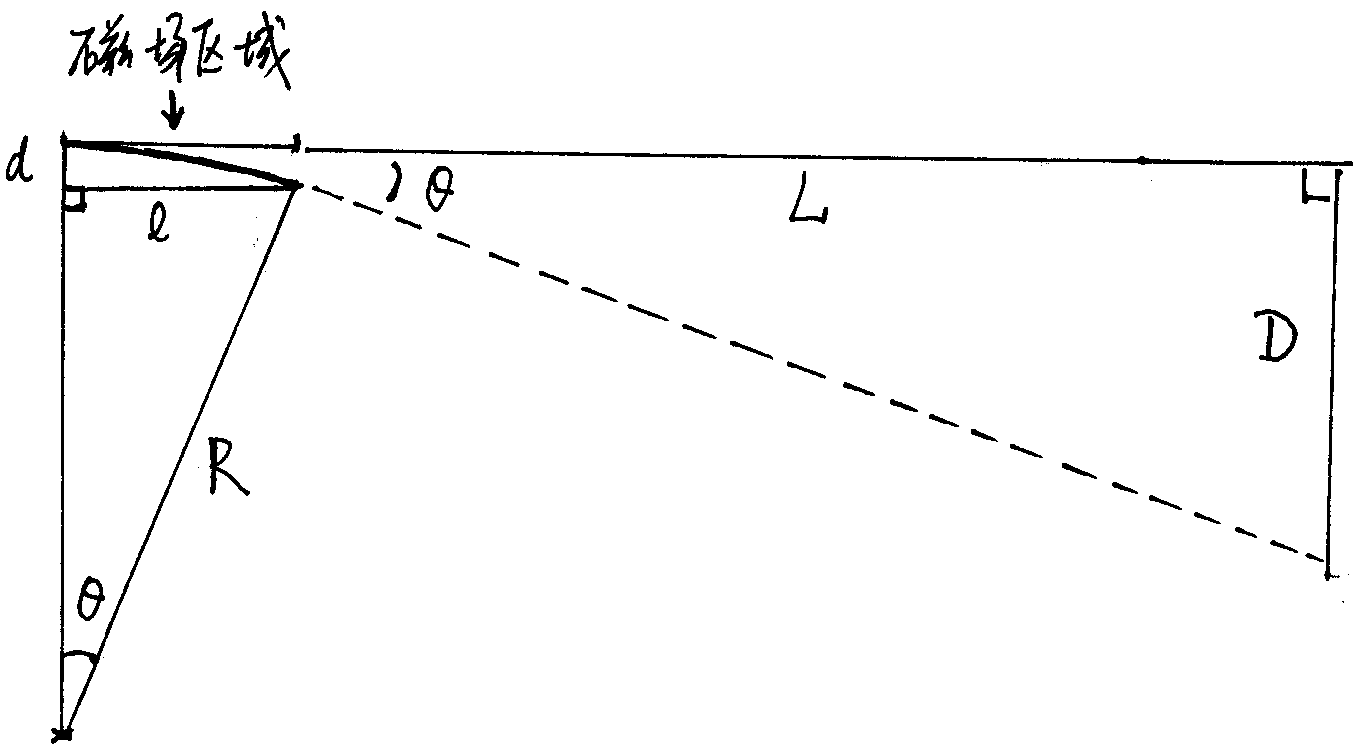
\includegraphics[width=8cm]{Duality/jjthompson.png}
\caption{汤姆逊实验。}
%\label{default}
\end{center}
\end{figure}

J J的方案是把阴极射线放出来,在经历了一个磁场区域后,再让它自由地飞一段,飞一段比较长的距离,这样偏转就会被放大。假设偏转角是$\theta$,阴极射线在水平方向上飞了距离$L$,最终在竖直方向的偏转是$D$,那么$D \approx L \theta$,即$L$越长,我们就越容易观察到偏转。

阴极射线发生偏转是因为它曾在磁场区域中运行过一段距离,假设这个距离是$l$,在这段距离里阴极射线会因磁场的存在,因洛伦兹力而偏转,偏转角度$\theta$满足如下关系:

\begin{equation}
R \sin \theta \approx R \theta = l 
\end{equation}

阴极射线在磁场里运行的时候也会有个偏转,记为$d$,这个偏转很小,很难被直接测量。但假如有这个$d$的话,线段$R - d$,$l$,$R$将构成一个直角三角形,因此有关系:

\begin{equation*}
(R-d)^2 + l^2 = R^2
\end{equation*}

化简后,可以求出:$R = \frac{l^2}{2 d}$,于是$\sin \theta$可以表示为:

\begin{equation}
\sin \theta = \frac{l}{R} = \frac{2d}{l}
\end{equation}

由于$\theta$很小,$\theta \approx \frac{2 d}{l}$。代入$D \approx L \theta$,$D \approx L \frac{2d}{l} $,求出:

\begin{equation}
 d = \frac{D l}{2 L}
\end{equation}

因此:

\begin{equation}
R = \frac{L l }{D }
\end{equation}

我们可以代入当年J J的数据来说明这个实验会碰到的困难。

在磁场区域中阴极射线飞了$ l = 0.05  $米,飞出磁场后阴极射线又继续飞了$ L = 1.1 $米,最终阴极射线在竖直方向上偏转了$ D = 0.07 $米。

由此我们可以估算:$d = \frac{ 0.07 \times 0.05  }{ 2 \times 1.1} = 0.0015 $米,即1.5毫米,确实很小,考虑到阴极射线本身撞在玻璃上会形成一个有限大小的光斑,这个偏转实际上是无法被测量的。

阴极射线在磁场中运动的半径是:$R = \frac{ 1.1 \times 0.05 }{ 0.07 } \approx 0.79$米,即将近1米,相比于$l = 0.05 $米(5厘米)或$D = 0.07$米(7厘米),确实很小。

但现在还有速度$v$不知道,如果假设阴极射线是个粒子的话,那它就可以以一个有限的速度$v$运动,为了把这个$v$表示出来,J J又使用了一个技巧,即加上一个竖直方向的电场,使带电粒子受一个与洛伦兹力正好相反的静电力,这时两个力就抵消了,偏转$D$将归零。

列出力的平衡方程:

\begin{equation}
q E = q v B
\end{equation}

因此:

\begin{equation}
v = \frac{E}{B}
\end{equation}

我们还是用J J当年的数据,电场强度$E = 1.0 \times 10^4 $牛/库,$B = 3.6 \times 10^{-4}$ 牛/安·米。

求出$v \approx 2.78 \times 10^7 $米/秒,将将是光速的十分之一,我们这里忽略相对论效应是安全的。

最终我们可求出:

\begin{equation}
\frac{m }{q } = \frac{B^2}{ E }  \cdot \frac{L l }{D}
\end{equation}

代入J J当年的数据,我们求出:

\begin{center}
$\frac{m }{q  } \approx  1.0 \times 10^{-11} $千克/库。
\end{center}

这个比值叫质量电荷比(Mass-to-charge ratio),但现在我们多用其倒数,即电荷质量比(charge-to-mass ratio),2010年CODATA推荐的数值是:

\begin{equation}
\frac{e}{m_e} = (1.758820088 \pm 39) \times 10^{11} C/kg
\end{equation}

J J 汤姆逊的实验是对粒子说的一大推动,自此之后大家就都倾向于认为在物质中存在着带负电的基本单元——电子(electron),我们把电子的质量记为$m_e$,把电子的电荷记为$e$(但我们需要记住电子所带电荷为负)

\subsubsection{油滴实验}

在汤姆逊实验之后不久,密立根又做了个油滴实验(Oil drop experiment),他把油滴通过小喷嘴喷进一个均匀电场里,在这个过程中,油滴会带上电,而电场的选择会给带电油滴一个向上的力,这个向上的力有可能与油滴本身的重力相互抵消。(必须提醒的是我们这里对实验的讨论是大大简化的。)通过显微镜我们可以找到那些“静止”的油滴,然后测出它们的直径$D$……

现在力的平衡条件是:

\begin{equation}
\frac{ \pi D^3 }{6} \rho g = Q E
\end{equation}

这里$\rho$是油滴的密度,$D$是油滴的直径,$E$是电场强度,它们都是实验可以测量的,因此我们可以确定油滴所带的电量$Q$,通过实验我们可以求出很多$Q$,由此我们再推测它们其中是否存在一个基本单元$e$。

假如我们没有“电子”的观念,我们是不可能做油滴实验的,因为这个实验就是假设物质中存在着一个基本的带电单元$e$,然后力争找到它,现在油滴所带电量可表示为$ Q = N e$,$N$是整数,这样通过列表我们可以推测出$e$的大小。

密立根的结果是:$e = - 1.592 \times 10^{-19}$库。与今天的结果:$e = −1.602 \times 10^{-19} $库比较差别不大。


科学活动某种意义下就是一个游戏,游戏要好玩、丰富才玩的下去。电子的粒子图像在迄今为止的实验中之所以能占上风,就是因为它更丰产,假设阴极射线是一种粒子,我们就能更有效地进行计算,对实验做出解释,并激发新的实验,并进而做出新的解释……更“丰产”就决定了粒子说会压倒波动说。

所以这里的关键并非是想象“电子到底是什么?”或“电子的图像到底是波还是粒子?”

而是要问:“电子存在的实验证据是什么?”“采用粒子图像我们能计算什么?”而“采用波动图像我们又能计算什么?”

我们通过手中的笔纸与实验生产出来的实验事实对话。


\subsubsection{光的粒子性}

19世纪末、20世纪初,物理学家普遍认为电子适用粒子图像,而光适用波动图像。但接下来情况又会有所变化,普朗克在解释黑体辐射的时候引入了量子概念,认为光在与物质发生能量交换的时候是以一份一份的方式进行的,每一份能量的大小是$h \nu$。

爱因斯坦在此基础上则干脆认为光也有个基本组成单元——光子——每个光子会集中地携带一份能量$h \nu$,并利用这个概念解释了光电效应实验。接下来我们就该问光子是否会像粒子那样携带动量了,考虑到光子速度是$c$,我们必须考虑相对论效应:

\begin{equation}
E^2 = c^2 p^2 + m_0^2 c^4
\end{equation}

这是适用于相对论的能量和动量的关系,$m_0$是静止质量,对光子而言$m_0 = 0$。公式可化简为:

\begin{equation}
E = cp
\end{equation}

考虑到光子的能量是$E = h \nu$,光子具有的动量就是:$p = \frac{h \nu }{ c }$,即:

\begin{equation}
p = \frac{h }{\lambda }
\end{equation}

在粒子的图像下,光将集中地携带一份动量,和一份能量,光子可以和其他粒子发生碰撞。在这个概念下,可以解释康普顿散射实验。

康普顿用一束X-射线(就是频率极高的光)照射在C原子上,由于X射线能量太高了,能量高,意味着频率$\nu$大,而频率$\nu$大则意味着波长$\lambda$小,因此入射的光子具有很大的动量。这么大能量-动量的光子会撞在C原子的某个外层电子上,相比于光子的大能量-动量,电子仅仅是被松散地束缚在原子核的附近,就好像是个被轻轻地放在一个浅坑上的高尔夫球,被飞速射来的另一个高尔夫球击中,这是一个标准的碰撞问题,光子的一部分能量-动量会转移给电子,其后果就是电子被撞飞,而光子会损失部分能量-动量,然后以某个特定的角度$\theta$被散射出去,这个散射角会和散射前后光子的波长有如下关系:

\begin{equation}
\lambda'  - \lambda  = \frac{h }{m_e c}  (1 - \cos \theta)
\end{equation}

这里$\lambda'$是散射后的波长,$\lambda$是散射前的波长,散射后X-射线的波长变长了。

\subsubsection{电子的波动性}

现在我们就有了这样一个序列:

起初,从古希腊到牛顿人们认为光是一种很细小的粒子,然后认为光是一种波动(托马斯·杨),再然后认为光是一种电磁波,被麦克斯韦方程组描述(赫兹实验),而现在从黑体辐射、光电效应到康普顿散射实验都表明“光的行为”像是个粒子。

但我们现在没法讨论关于光的量子理论,这涉及到对电磁场的量子化。我们只是回顾了一下潮流,关于光的观念就像时尚界的潮流,先是粒子、然后是波动,最后又回到粒子。

这种历史性的考察启发了一位专业本来是历史学的物理学家——德布罗意——他认为既然传统上被认为是波动的对象可以在某些实验里像粒子,那么传统上被认为是粒子的对象——比如电子——它是否也可被认为是波动呢?这就把我们带到了波动力学的门槛。

首先我们需要建立一个翻译,即由粒子的语言翻译到波动的语言,粒子的语言里我们有动量$p$,而在波动里我们有波长$\lambda$,德布罗意由氢原子的玻尔模型出发,猜出了一个联系:

\begin{equation}
\lambda = \frac{h }{p }
\end{equation}

利用普朗克量子化条件$E = h \nu$,我们还可把能量$E$翻译为频率$\nu$:

\begin{equation}
\nu = \frac{E }{h }
\end{equation}

以上两个等式对电子适用,对光子也适用。某种意义上我们可以把它们看做是从光子到电子的推广。

在波矢$k = \frac{2 \pi }{\lambda}$和角频率$\omega = \frac{2 \pi }{T }$的定义下,使用波动语言,我们把一个能量为$E = \hbar \omega$,动量为$p = \hbar k$的粒子表示为一个波:

\begin{equation}
\psi( x, t ) A \cos ( k x - \omega t )
\end{equation}

或写为复数的形式:

\begin{equation}
\psi (x,t ) = A e^{i ( k x - \omega t )} = A e^{\frac{i }{\hbar } (p x - E t) }
\end{equation}

这种波被称为德布罗意波或物质波(matter wave)。既然电子是波,那么电子也应该有干涉/衍射效应\footnote{这里,干涉一般被定义为两列波相加,而衍射一般被定义为很多列波相加。}。

1925年,戴维逊和革末(Davisson \& Germer)在做电子在镍单晶上散射实验时,第一次观察到了电子在晶体中的衍射效应。

\begin{figure}[htbp]
\begin{center}
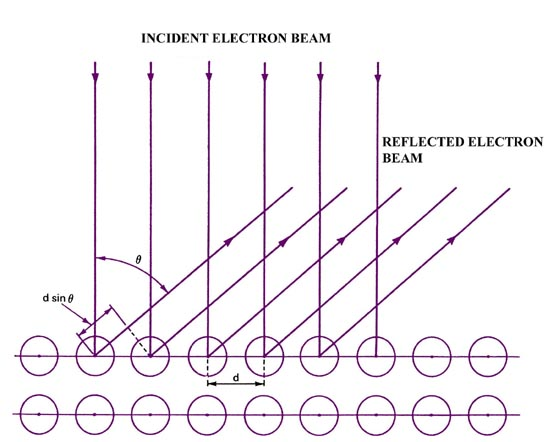
\includegraphics[width=8cm]{Duality/davisson.jpg}
\caption{电子在晶格上的衍射。}
%\label{default}
\end{center}
\end{figure}

假设电子由正上方垂直入射到镍晶体上,所谓晶体是原子的周期性排列,我们把每个原子都想象为一个障碍物,当电子如波一样撞到原子上时就和水波撞到芦苇上一样,我们可把障碍物看做是个新的波源,波撞在障碍物上然后向四面八方发射出去。

这时晶体上的每个格点都是一个新的波源,假设格点间的间距是$d$,或说假设晶格中存在着以$d$为周期的平移对称性,我们就可以构造如图一束束垂直入射,然后向某个方向$\theta $散射的电子波束。

我们考虑相邻的两列向$\theta$方向散射出去的波,然后计算它们之间的相位差。波动的相位和$(k x - \omega t)$有关,$t$是时间,对大家都一样,那么相位差就只和$x$有关。如图两列波走过的路程是不一样的,它们都由上方的无穷远入射,出射到$\theta$方向的无穷远去。

因此路程差是:

\begin{equation}
d \sin \theta 
\end{equation}

假设相邻两列波的路程差正好是一倍的波长:

\begin{equation}
d \sin \theta = \lambda
\end{equation}

或:

\begin{equation}
\theta =  \sin^{-1} \frac{\lambda }{d }
\end{equation}

我们将能观察到一个波峰遇波峰的情况,即相干地加强!如果物质波的波长$\lambda$和晶格的间距$d$差不多,我们会比较容易观察到这个波的加强。

假设不考虑电子的相对论效应,自由电子的能量是:

\begin{equation}
E = \frac{p^2}{2 m}
\end{equation}

电子的动量是:

\begin{equation}
p = \sqrt{ 2 m E  } = \frac{h }{\lambda }
\end{equation}

我们可估计出电子入射的能量:

\begin{equation}
E = \frac{ h^2 }{ 2 m \lambda^2 }
\end{equation}

计算出来的结果是$2.4 \times 10^{-17} $焦耳,或$150$电子伏。


\subsection*{练习}

\begin{enumerate}
\item 

在一个恒星系统中,行星离恒星越近它的温度就越高,反之则温度越低,我们可以针对特定恒星计算它的宜居带,即围绕恒星的带状区域,离恒星既不近也不远,温度正好处于$0-100 {}^o C$之间。

现在已知有这样一颗恒星Kepler-186(主序M1-型矮星),它的表面温度是3788开尔文,半径是0.47倍太阳半径,质量是0.48太阳质量。

求:(a)这颗星的颜色;(b)它的宜居带——即使行星表面温度处于$0-100 {}^o C$之间——距离恒星的最近和最远距离。


\item

由黑体辐射公式导出维恩位移定律:能量密度极大值所对应的波长$\lambda_m$与温度$T$成反比,即:$\lambda_m T = B$,$B$是一常量,近似计算$B$的数值。

解: 由频率的分布$\int u_T(\nu) d\nu$出发:

\begin{equation*}
\int u_T(\nu)d\nu =\int  \frac{8\pi h
\nu^3}{c^3}\frac{1}{e^{\frac{h\nu}{k_B T}} -1} d \nu
\end{equation*}

变量变换,把$\nu \to \lambda$, $\lambda = \frac{c}{\nu}$, $d \lambda = - \frac{c}{\nu^2} d \nu$. 或:$\nu = \frac{c}{\lambda}$, $d\nu = - \frac{\nu^2}{c} d\lambda=-\frac{c}{\lambda^2}d\lambda$。

\begin{equation*}
\int u_T(\nu) d \nu = \int \frac{8\pi
hc}{\lambda^5}\frac{1}{e^{\frac{hc}{k_B T\lambda}}-1} d\lambda
\end{equation*}

上式中我们把负号“-”略去不写. 现在对新的$\int u_T(\lambda)
d\lambda$中的$u_T(\lambda)$求微分. 极值条件:

\begin{equation*}
\left. {\frac{d u_T(\lambda)}{d\lambda}} \right|_{\lambda =
\lambda_{max}} = 0
\end{equation*}

令: $x = \frac{hc}{k_B T \lambda}$, 上式化简可得:

\begin{equation*}
(5-x)e^x =5
\end{equation*}

这个方程可通过``作图法''求解\footnote{Mathematica:
``FindRoot[5*Exp[x]-x*Exp[x] ==5 , \{x,10\}]''

``解析解'', 网址:

\url{http://www.udel.edu/physics/csaapt/Fall2002/files/analytic-solutions.doc}},

解出: $x \approx 4.97$, 即:

\begin{equation*}
\frac{hc}{k_B T \lambda_{max}} = 4.97
\end{equation*}

即:

\begin{equation*}
    \lambda_{max} T =\frac{hc}{4.97 k_B} = 2.898 \times 10^{-3} m \cdot K
\end{equation*}

值得注意的是如果我们由$\int u_T(\nu) d \nu$出发, 对$u_T(\nu)$求偏导, 即: $\left.{ \frac{d u_T(\nu)}{d \nu}} \right|_{\nu = \nu_{max}}= 0$, 所求出的$\nu_{max}$与$\lambda_{max}$不是一个“颜色”,即这样定义的$\lambda_{max} \nu_{max} \neq c$。

令$\frac{h\nu}{k_BT} = x $,由$\left.{ \frac{d u_T(\nu)}{d \nu}} \right|_{\nu = \nu_{max}}= 0$得到:

\begin{equation*}
    (3-x)e^x = 3
\end{equation*}

利用Mathematica中的FindRoot命令

\begin{verbatim}
    FindRoot[3*Exp[x]-x*Exp[x]==3, {x,10}]
\end{verbatim}

解出: $x \approx 2.82 $, 即:


\begin{equation*}
\frac{h\nu_{max}}{k_BT} = 2.82
\end{equation*}

\end{enumerate}




\newpage

\section{波动力学}


\subsection{波粒二像性}


我们对粒子和波动的概念来自直接的经验。和粒子有关的经验对象:小到石子大到天上的星星等;和波动有关的经验对象:最常见的例子是水波,还有拨动的琴弦等。但这些还不是物理中所说的模型,物理中所谓粒子和波动是理想化的模型,是我们头脑中抽象的对象。


\subsubsection{粒子的图像}


在经典物理中,粒子的概念可进一步抽象为:大小可忽略不计的具有质量的对象,即所谓质点。质量(mass)在这里是新概念,mass的原初含义就是多少,这里引申为对物体惯性质量多少的量度。一个西瓜,比西瓜籽的质量大,因为西瓜里包含的物质比西瓜籽多,西瓜保持自身运动状态的能力比西瓜籽强。

为叙述的简单,我们现在可把粒子等同于质点。要描述一个质点的运动状态,我们需要知道其位置$x$和速度$v$,速度是对位置的微分。

\begin{equation}
v = \frac{d x}{d t}
\end{equation}

这是莱布尼茨的记号,我们有时也把它记为$\dot x$,$\dot x$是牛顿的记号。记号会有助于我们思维,比如$\dot x$比较简短,而$frac{d x}{d t}$则会提醒我们微分运算的结构,即微分是如何定义的,粒子在时间$\Delta t$内飞行了$\Delta x$,然后我们对$\Delta t$取极限。

而取极限是构造这样一个可以count的过程,(1)首先,$\Delta t = 1$秒;(2)$\Delta t = 0.1$秒;(3)$\Delta t = 0.01$秒;(4)……。假设运算$\frac{\Delta x }{\Delta t}$在这样一个可以count的过程里趋于一个确定的数,我们就说极限存在。

我们研究数学是为了应用于物理的研究,而物理研究的对象都是确定的现象,这决定了我们特别对这类数学形式感兴趣,比如在这里就是极限存在,如果极限不存在,我们也要努力调整数学结构使其存在,否则我们正在使用的数学对物理研究就是不趁手的。

对时间做微分就必须讨论时间,时间也是一个直观的概念,这里我们可把时间描述为一个时钟,我们会发现当指针指到不同位置时,质点的位置可能不同,于是指针的位置就定义了时刻$t$。有了时刻$t$,我们对质点的描述就变成了$x(t)$,在想象中动起来的质点就是一条线,就是轨迹。由$x(t)$可定义速度$v(t)$,考虑到质点还有质量$m$,我们现在用位置$x$和动量$p$这一对量来表示质点的运动状态。

$x$和$p$并放$(x, p)$就是相空间(phase space)中的一个点。相空间是抽象的数学空间,比如在这里我们要描述一个粒子的运动,位置是三维的($x, y, z$),动量也是三维的($p_x, p_y, p_z$),相空间就是六维的。我们用六维超空间中的一个点来描述一个质点的运动。

在日常经验中我们还有相互作用或所谓力的概念,我们在地球上拎起不同质量物体时肌肉的紧张程度是不同的,或者说在地球上用弹簧秤拎起不同质量物体时弹簧的拉伸程度是不同的。

以上我们对质量、时间、力等的定义都是直观的,是可以操作的。按照以上思路进行研究,研究落体的运动,研究天体的运动,……最终诞生了牛顿的经典力学。这里我们可简单地用两个公式:$F=ma$(牛顿第二定律)
和$F = \frac{GMm}{r^2}$(万有引力公式)
来代表牛顿力学。前者是质点的运动方程,用数学的语言说是一个关于位置$x$的二阶微分方程,根据微分方程的理论,只需要知道初始时刻$t=0$时的位置$x$和速度$v$即可求出以后任意时刻$t$质点所处的位置,即轨迹$x(t)$。

需要强调的是一旦我们知道$t=0$时$x$和$v$的精确值(没任何误差),$x(t)$的取值也是精确的,即我们得到的是对质点未来演化的精确预测,并且这个求解对$t < 0$也精确成立,这意味着我们还可精确地反演质点的历史。这些结论是由牛顿力学的数学结构严格保证的,即轨迹是一根理想的线,它没有宽度。

现在我们就有了一个关于世界的整体图像:宇宙是由很多质点构成的复杂系统,它们两两之间的相互作用由$F=\frac{GMm}{x^2}$决定,对每一个质点我们又可列出$\sum\limits_i F_i = ma$这样的运动方程,$\sum\limits_i
F_i$表示质点所受的合力,与其他质点的位置有关,因此这是一个联立的二阶微分方程组。

还是根据数学的理论,如果我们知道了初始时刻$t=0$时每个质点的位置和速度,我们即可无限精确地知道系统内每个粒子的轨迹。这在哲学上被引申为所谓的“决定论”,我们会倾向于相信:世界只不过是个巨大的机械,人生的命运是确定的,事物的演化也是确定的等等。

当然要想在某一时刻同时测量出全世界所有粒子的位置和速度是不可能的,但这是否意味着——“某一时刻全世界所有粒子具有确定的位置和速度”——本身就不存在呢?有些人可能会持怀疑的态度。另一些人会倾向于相信,当然这种相信并无充分的证据,相信的好处是我们可建立起一个关于世界的整体图像,整个世界变得有秩序了,可以理解了。

不管我们是否相信决定论,牛顿力学本身获得了巨大成功,解释了大到行星运动,小到苹果落地等广泛的现象,因此主流物理学家在100多年前相信牛顿力学提供了描述整个世界的基础。

\subsubsection{波动的图像}

在有了粒子的图像后,我们很容易把波动还原为很多粒子的集体运动。比如最简单的波动,抖动绳子可产生一维波。要解释这样的波动现象,最简单的模型就是假想把绳子分成很多很多份,每部分很小以至我们可将其视为质点,质点间的力用弹性力表示。看起来这就是一根弹簧,上面放了很多等质量的小球,如果你横向摇晃第一个小球,这种运动就会渐次地传递给其他小球,像墨西哥人浪一样,波行进的方向和小球偏离的方向垂直,即所谓横波;如果你纵向压缩拉伸第一个小球,这种纵向的振动也会渐次地传递给其他小球,即所谓纵波,纵波的例子是声波。

由此可见波动是一种整体运动,是由很多粒子参与步调统一的运动。最简单的波动是单色平面波,即体现为正弦或余弦函数:$A\cos(kx - \omega t)$。波动的特点是会传播出去,因此你很难说波在什么地方,或说了也没啥意义,因为它无所不在。对单色平面波来说,波动在每一点的状况都是一样的,但我们可以发现相邻波峰间距离总是相同的,于是可定义波长:$\lambda$,我们还发现每个质点振动一个周期的时间也是相同的,因此可定义频率:$\nu$。

很多质点的整体运动——“波动”——和“粒子”是很不同的,描述粒子的运动,使用位置和动量,描述波动使用振幅$A$、波长$\lambda$和频率$\nu$。粒子的特点是分立的,每个粒子会集中地携带能量$E$和动量$p$,而波动的特点则是弥散的,能量会均匀地分布在介质(中的每个质点)上,波动的能量密度正比于振幅的平方($A^2$)。

粒子是分立的,它们各自在虚空中运行,互相用引力勾连着;而波动是连续的、充盈的整体运动,由波动方程描述。从这个意义上我们说粒子的图像和波动的图像是排斥的,即我们无法想象一个对象既是粒子又是波动。

\subsubsection{电磁波}

尽管粒子的图像和波动的图像是互相排斥的,我们仍会认为粒子的图像更本质,波动的图像可还原为粒子的语言,因此是从属的。但物理学家很快又发现了一种新的波——电磁波。

电磁现象是不同于机械力学(即上面讨论的质点或质点系的运动)的新现象。麦克斯韦是电磁学中的牛顿,他提出的麦克斯韦方程组是解释电磁现象的基础。利用麦克斯韦方程组最重要的预言是“光波就是电磁波”或“电磁波就是光波”。

所谓电磁波就是电场($E$)和磁场($B$)在空间中的传播,和机械波中质点振动会在空间中传播一样,它们都满足类似的波动方程,只是波动传播的速度不同而已。

物理学家自然提出一个任务,即能否把电磁波还原为纯粹的机械运动?追求统一的物理是物理学家永恒的追求,牛顿使天上的物理(行星运动)和地上的物理(苹果落地)统一,麦克斯韦使光学和电磁学统一,那么经典力学和经典电磁学也应该是统一的。但实际上把电磁波还原为机械运动的努力一直没取得啥进展。

如果考虑到光波或电磁波无法还原为机械运动,我们现在可说粒子的图像和波动的图像在概念上是同等重要的,但在量子场论中,粒子被解释为场的激发,这有点把粒子还原为场的意思。

\subsection{双缝实验}

量子力学诞生于原子物理学,即关于原子尺寸物理现象的研究。今天我们知道原子大约是0.1纳米,而人类肉眼可分辨(假设可借助光学显微镜)的尺寸大约是可见光波长的数量级——几百纳米,即我们研究的对象小了至少几万倍。从这个意义上说量子现象是超越于我们日常经验之外的。当我们提到粒子和波动的时候,即便没有系统地学习过物理学,我们也可借助日常经验在“望文生义”的意味下知道粒子大致指的是什么现象,波动指的是什么现象。但当我们讲到原子或电子的运动时,我们就没有这样的直观了。

~

所以如果不系统地补足物理学史上关于原子物理的研究的话,就必须得有一个机会供我们直观地体验一下量子现象。费曼曾提出著名的双缝实验\footnote{费曼提出单粒子双缝实验时并未真的试图实现它,但随着技术的进步现在已有物理学家完成真正的单电子双缝干涉实验:\url{http://physicsworld.com/cws/article/print/9745}},通过这个实验我们可建立量子力学的基本概念——波粒二像性。

在光学中也有双缝实验,光通过双缝,绕过障碍物,互相叠加,最终在屏上呈现出明暗相间的条纹状分布,这个被称为干涉。干涉现象很容易用波动的图像解释:光是电磁波,当波照射到双缝上时,每个缝相当于是新的波源(惠更斯原理),每个波源都会发出一系列波峰和波谷,当两个波峰相遇时则加强呈现出明亮的条纹,当一个波峰和一个波谷相遇时则抵消呈现出暗条纹。

\begin{figure}[htbp]
\begin{center}
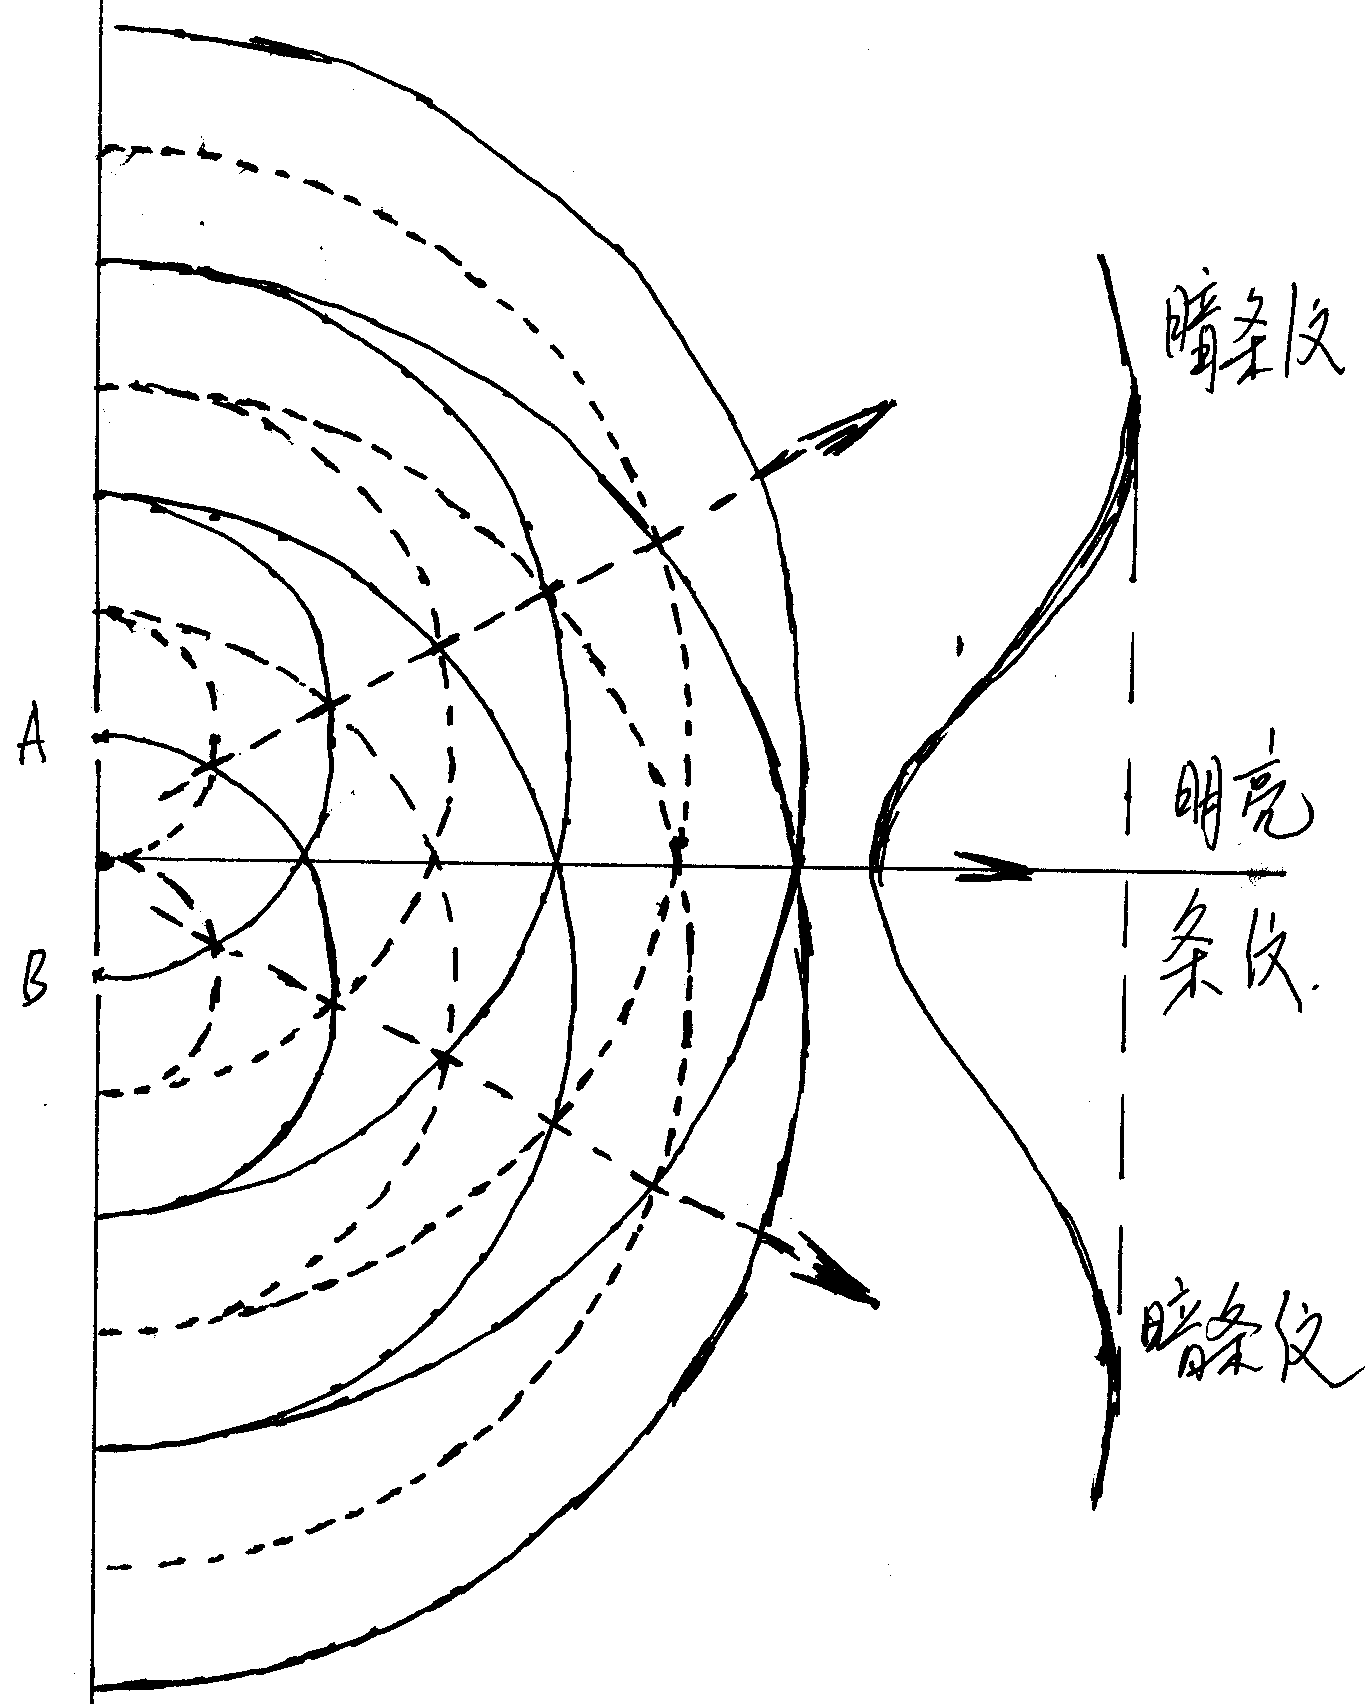
\includegraphics[width=10cm]{QuantumIntro/doubleslit.png}
\caption{双缝干涉示意。}
%\label{default}
\end{center}
\end{figure}

现在我们假设以一束电子入射到双缝上,看看会发生什么现象。电子是量子力学对象,但现在我们先猜测它就是经典的粒子,这种情形下电子穿过双缝——呈上、下两个条状分布。费曼讲的是机枪扫射,看子弹如何穿过双缝,根据日常经验子弹无法绕过障碍,将集中地分布在双缝的方向上。

那么实验的结果是什么呢?是明、暗相间的条纹状分布,就好像光学中的双缝实验结果一样。这是否意味着电子是一种波动呢?就像迄今为止我们都理所当然地认为光就是一种波动,一种电磁波。

我们可以再做实验,让电子一个、一个地通过双缝,看看是否会有干涉现象。实验结果是电子将随机地出现在任意位置,我们根本无法预测电子下一次出现在什么位置。但我们也注意到电子并未弥散开来,每次都只出现在一个位置,这说明电子还是粒子。另外一个特点是当我们进行很多次这样的单电子双缝干涉实验后,电子的总体分布会趋于明暗相间的干涉条纹。

有趣的是,对于我们一直认为是波动的“光”,我们也可完成类似的实验,即当我们降低光的强度,最终我们发现光竟然也是由一个一个的粒子——“光子”组成的。当光强极弱时,我们可完成所谓“单光子干涉实验”,单光子穿过双缝对应一个随机的位置,很多单光子事件累积起来呈现干涉条纹。实际上人眼就是理想的“单光子”探测器,生理实验表明只需要5个光子就可使视杆细胞兴奋。

因此,把电子(或光子)简单地设想为经典的粒子或经典的波动都是不可能的,现在我们说电子(或光子)首先是粒子,但它不是经典的,它的运动状态不能用位置$x(t)$和动量$p(t)$描述,而需要用波函数$\psi(x,t)$来描述。这就是所谓波粒二像性,这与日常经验中的粒子是两回事,但物理学家们一般还称呼它们是粒子。

\subsection{波函数}

根据量子力学,粒子的运动状态是由波函数来描述的,其实经典的波动也是由波函数来描述的。量子力学中的波
函数和经典波动波函数的区别在于:经典波动波函数有确切的物理含义,比如电磁波波函数表示的是变化的电场或磁场;量子力学中波函数不对应确切的物理含义,
它一般是复函数,而物理量(如位置、动量)的取值是实数,但物理系统中所有信息却又都包含在波函数中,即根据波函数我们可求出物理量的取值。从数学形式上
看波函数很类似经典波动的波函数,因为经典波动为计算方便也常常表示为复函数的形式;而量子力学中波函数在某些特定情况下也可表示为实函数的形式。这给思考量子力学问题带来很多直观上的好处,因为想象一个经典波动总是很容易的。

最简单的波函数是单色平面波(plane wave):

\begin{equation}
\psi_k (x, t) = A e^{i(kx -\omega t)}
\end{equation}

它所描述粒子的动量是:$p = \hbar k$,能量是:$E = \hbar
\omega$(前者是德布罗意的贡献,后者是普朗克的贡献)。动量的表达式很有用,稍作变形:

\begin{equation}
\lambda = \frac{h}{p}
\end{equation}

这个公式代表了波动语言(左边)和粒子语言(右边)的“翻译”关系。

如前所述,波函数本身——是个复数——没有物理意义,但其绝对值的平方——$\psi^* \psi $是个实数——代表发现粒子的几率密度,这叫做波函数的统计解释(或玻恩解释)。

如果要使得波函数的模方$\psi^*(x) \psi(x)$就是几率密度$\rho(x)$,我们就必须把波函数归一化(Normalization),使得:

\begin{equation}
\int \psi^* \psi dx =1
\end{equation}

粒子的平均位置是:

\begin{center}
粒子的位置 $\times$ 粒子在某处的几率
\end{center}

表示为数学的式子:

\begin{equation}
\overline{x} = \int x | \psi(x) |^2 dx = \int \psi^*  x \psi  d x
\end{equation}

量子力学中还有一条基本原理——“态的叠加原理”(或波函数的叠加原理):

\begin{quote}
如果$\psi_1$代表物理系统一个可能的态,$\psi_2$代表另一个可能的态,那么$c_1\psi_1 + c_2\psi_2$也是一个可能的态。(这里$c_1$,$c_2$是任意复数)
\end{quote}

利用“波函数的统计解释”和“态的叠加原理”,可以很容易理解费曼双缝实验,单电子通过双缝,可用如下波函数表示:

\begin{equation}
\psi  = \psi_1 +  \psi_2
\end{equation}

这里的1和2并不是表示1、2两个电子,单电子意味着只有一个电子,$\psi_1$和$\psi_2$都是这个电子波函数的一部分,1 对应的是上缝,2对应的是下缝。电子的几率分布为:

\begin{equation}
\left( \psi_1^* + \psi_2^*  \right) \left( \psi_1 + \psi_2  \right) = |\psi_1|^2 + |\psi_2|^2 + \psi_1^*\psi_2 +
\psi_1\psi_2^*
\end{equation}

这相当于经典光学中两束光波的迭加,体现为明暗相间的条纹,从数学上说它是由干涉项$\psi_1^*\psi_2 + \psi_1\psi_2^*$导致的。

假设:$\psi_1 = |\psi_1| e^{i \theta_1}$,$\psi_2 = |\psi_2| e^{i \theta_2}$, 则:

\begin{equation}
\psi_1^* \psi_2 + \psi_1 \psi_2^*  = 2 |\psi_1 | \cdot | \psi_2 | \cos (\theta_1 -\theta_2)
\end{equation}


\subsubsection{测量}


我们继续对最简单的波函数:$A e^{i(kx - \omega t)}
$做一些讨论,假设我们设法测量一下粒子的位置$x$
\footnote{利用超快光学测量电子运动的最新进展:\url{http://focus.aps.org/story/v21/st7}
这里是通过制备很多相同电子波函数,然后测量不同阶段电子的位置来获得电子运动图像的,并非是对相同电子运动的持续测量。}。

根据统计解释,波函数绝对值的平方是粒子的分布几率,由于波函数的振幅是常数,粒子是等几率分布的,因此我们可能在空间中任意地方等几率地观测到粒子。那么对于一次具体的测量,粒子将出现在何位置?我们没法预测,只知道会在空间任何地方。

暂不讨论我们是如何测量粒子位置的,假设$t=0$时我们完成了一次成功的测量,我们会观测到粒子在某确定位置$x=x_0$
,现在我们问:在$t=0$之前的一瞬间粒子在什么地方?关于这个问题有两种答案\footnote{关于波函数统计解释和波函数坍缩更详尽的讨论可参考:D. J. Griffiths, Introduction to Quantum Mechanics, pp2-5;}:

\begin{figure}[htbp]
\begin{center}
\includegraphics[width=8cm]{QuantumIntro/peak_atx0.ps}
\caption{假设$t=0$完成一次成功的测量,测得粒子在$x=x_0$附近;}
%\label{default}
\end{center}
\end{figure}


\begin{enumerate}
\item 

虽然我们无法精确地知道粒子在什么地方,但我们可推测其一定在$x_0$附近,因为根据狭义相对论,粒子运动速度存在一上限,因此在测量前一瞬间,粒子应在$x_0$附近。那么在测量前一瞬间,波函数还是单色平面波吗?因为我们考虑的是测量前,在此操作前波函数无任何理由发生变化,因此应当仍然是单色平面波。但根据量子力学统计解释,粒子应等几率地分布在整个空间,而不是仅仅分布在$x_0$的附近。看来根据量子力学无法得到关于粒子的全部信息,从这个角度说量子力学是不完备的。因此一定还存在某种未知因素,决定了粒子以何种方式在$x_0$附近,因为不知道该因素到底是什么,我们就管它叫隐变量(hidden variables)。这是对量子力学的一种态度,即认为量子力学是不完备的,我们需要发展一种新理论取而代之。持这种观点的物理学家有爱因斯坦、玻姆等。

\item

这一派物理学家认为基于波函数和统计解释的量子力学是完备的,我们可称之为正统派,对创建量子力学有直接贡献的玻尔、玻恩、海森堡等都属于这一派。正统派提出“波函数坍缩”来描述量子力学的测量过程。测量前是单色平面波,粒子等几率地处在整个空间,一次成功的测量意味着在这一瞬间,波函数坍缩为一位置在$x_0$附近的尖峰形函数(数学上叫$\delta$函数,$\delta$函数仅在$x_0$取值不为0,其他地方都是0)。根据统计解释,粒子只能在$x_0$位置,自然这是一次成功的测量,因为我们得到了唯一的位置,在$t=0$之后,我们再做测量,也只能获得$x_0$这一确定性的结论,因为尖峰函数再坍缩也只能是尖峰函数。那么正统解释是否意味着与狭义相对论矛盾呢?或者说我们是否可利用波函数坍缩来构造一个可以携带信息的超过光速的信号呢?仔细的分析否定了这种设想,在这里我们暂不展开讨论。对这个问题的深入讨论引发了量子信息这个前沿领域。

\end{enumerate}

这两派意见,到底哪一派正确呢?贝尔后来针对隐变量理论提出了一个不等式——贝尔不等式,如果隐变量理论成立,不等式成立;如果正统解释成立,则不等式可以不成立。但迄今为止的各种实验对隐变量理论都是不利的,或者说量子力学是完备的,波函数中包括了粒子运动的所有信息。

\subsubsection{经典和量子的界限}

物理学家的基本信念是只有一个物理。原来经典物理可以描述的物理现象,比如行星的运动和几何光学也适用于量子力学。原则上量子力学应适用于所有的物理现象,只是对这些问题的处理会比较繁琐而已,而且经过繁琐的计算我们会发现奇异的量子效应被抵消掉了,这解释了为什么我们使用“错误”的经典理论也能得到正确的结果。

此外物理学是非常灵活,具有实用和工具精神的,当我们面对复杂问题时,大胆地舍去次要因素,只考虑主要因素并得到一个简单有效的算法始终是物理学的核心,而这么做的核心是发现看待事物的新角度,即简单有效是基于新形式的发现和新类的发现。严格求解或回答形而上学意义下僵硬的“是”的问题(比如“电子到底是波还是粒子”)从来不是物理学的趣味。

讨论经典和量子的界限\footnote{关于量子和经典的界限,可继续阅读:\url{http://physicsworld.com/cws/article/print/21590}},目的并不是给出经典物理和量子物理分别适用的界限(只有一个物理),而只是在讨论什么时候必须使用量子力学,或什么时候量子效应不可忽略。

我们可以用一个简单的计算来讨论,量子效应比较明显意味着我们必须用波函数描述粒子,意味着干涉效应比较明显。回忆公式:$\lambda = \frac{h}{p}$,左边是描述波动性的波长,如果波动性较明显,说明波长应比较长,比如说达到几百纳米(达到可见光波段)。这意味着等式右边:$h$必须越大越好,$h$是普朗克常数,恰恰是个很小很小的物理量,这解释了为什么我们平时观察不到量子效应。$p$是粒子动量,应越小越好,但再小也有上限,宏观物体普遍存在无规则热运动,无规则热运动能量可使用$E=k_B T$来估计(即温度越高,无规则热运动越激烈,这也与我们的常识吻合)。现在$p= \sqrt{2 m k_B T}$,$k_B$是另一个物理常数——玻尔兹曼常数,

\begin{equation}
k_B = 1.3806488 \times 10^{-23} J/K
\end{equation}

我们可讨论:

\begin{enumerate}
\item 

m越小越好,这解释了为什么我们会在原子系统中观察到量子现象,因为原子足够小;

\item

另一方面$T$(温度)越低越好,这解释了为什么在低温条件下我们会观察到宏观量子现象,比如超导、超流、超固体\footnote{“超级固体”(super solid)是个很新的研究领域,生活大爆炸中的谢耳朵曾提到过。}和玻色凝聚等。

\end{enumerate}

\subsection{薛定谔方程}

根据量子力学,系统状态是由波函数描述的,假设我们知道某时刻系统的波函数$\psi(t_0)$,我们希望知道系统是如何随时间演化的,即知道未来某时刻的波函数$\psi(t)$。波函数随时间演化的规律是由薛定谔方程给出的:

\begin{equation}
i \hbar \frac{\partial \psi}{\partial t} = \hat H \psi
\end{equation}

这里$\hat H$是哈密顿算符。

薛定谔方程可能是物理学中最重要的方程,其地位很类似于牛顿力学中的牛顿第二定律$F=ma$。它们都是描述随时间演化的动力学方程,不同之处在于牛顿第二定律中的加速度是对时间的二阶微商,因此需要知道初始时刻的位置$x_0$和速度$v_0$才可求解,而薛定谔方程中出现的是对时间的一阶微商,因此只需要知道$\psi(t_0)$就可确定$\psi(t)$。牛顿第二定律和薛定谔方程都是确定性的方程,一旦初始条件确定了,未来的演化是唯一确定的,不同的是牛顿力学中求出的是轨迹,而量子力学中求出的是波函数。轨迹代表了可视化的物理运动(比如开普勒的椭圆),而波函数则是一个复函数并不直接对应任何实际物理量。

但我们又说波函数中已经包含了物理系统的所有信息,因此我们关心的物理量(也称观测量或力学量)可通过特定的数学步骤由波函数导出,当然并非所有经典力学中可获得的信息在量子力学中也可获得。比如:我们在量子力学中无法同时获得一个粒子的位置和动量的取值,但在经典力学中我们是可以获得的。

考虑到两种理论内在的数学结构不同,有这样的区别应该也不算太出乎我们的意料吧。

%%%

\subsubsection{算符}

考虑最简单的波函数——单色平面波——$\psi = A e^{i(kx - \omega t)}$。波函数在任意$x$的取值是复数,并不对应具体物理量,但其绝对值$\rho(x) = \psi^* \psi $ 表示粒子处在$x$位置的概率密度。因此我们虽然无法由$\psi$预测$x$的具体取值,但可计算$x$的平均值(期望值):

\begin{equation}
\overline{x} = \int \psi^* x \psi dx = \int x \rho(x) dx
\end{equation}

我们可以把这样的数学步骤推广为:

\begin{equation}
\bar A = \int \psi^* A \psi dx,
\end{equation}

这里$\bar A$ 表示力学量$A$的期望值,$\hat A$叫做算符。算符是某种抽象的数学操作,它可把一个波函数$\psi(x)$映射为另外一个波函数$\phi(x)$,即:

\begin{equation}
\phi(x) = \hat A \psi(x)
\end{equation}

为了理解算符$\hat A$,我们可以把上式与函数的定义进行类比,函数的定义是:

\begin{equation*}
f: x \to y ,
\end{equation*}

即由定义域中的某数$x$按照规则$f$映射到值域中的某数$y$, 记作: 

\begin{equation*}
y = f(x)
\end{equation*}

算符也是映射,但它是把特定函数空间(数学上叫希尔伯特空间)中的一个函数$\psi(x)$,按照规则 $\hat A$ 映射到函数空间中的另一个函数$\phi(x)$,即:

\begin{equation*}
\hat A: \psi(x) \to \phi(x)
\end{equation*}

记作:

\begin{equation*}
\phi(x) = \hat A \psi(x) .
\end{equation*}

可见,对位置算符而言:

\begin{equation}
\hat x = x
\end{equation}

但并非都这样简单。比如对动量$p$,我们知道单色平面波$\psi_k = A e^{i(kx -\omega t)}$对应的动量是$p =\hbar
k$,只有一个确定的取值。如果取:

\begin{equation}
\hat p = \frac{\hbar}{i} \frac{\partial}{\partial x},
\end{equation}

可以验证:

\begin{eqnarray}
\hat p \psi_p &=& \hbar k \psi_p \\
\bar p &=& \hbar k
\end{eqnarray}

类似, 可验证能量算符为:

\begin{equation}
    \hat E = i \hbar \frac{\partial }{\partial t}
\end{equation}

它使得:

\begin{equation}
i \hbar \frac{\partial }{\partial t} \left( A e^{i (kx-\omega t)} \right)= \hbar \omega A e^{i (kx-\omega t)} ,
\end{equation}

像这样的方程叫作本征方程(eigen equation),抽象地写,就是这样的:

\begin{equation}
\hat A \psi_{\lambda}(x) = \lambda \psi_{\lambda}(x)
\end{equation}

其中$\lambda$是个数,一般来说是复数(complex number),本征方程就是要使得$\hat A \psi$仍然等于$\psi$ “自己”再乘上一个复系数“$\lambda$”,“eigen”一词在德语中就是“自身的”意思,因此这个“命名”是很形象的。这里$\lambda$叫本征值(eigen value),$\psi_{\lambda}(x)$叫本征函数(eigen function)。求解本征方程的过程叫“本征值问题”。

在量子力学中,我们都是用“厄米算符”去表示力学量的,“厄米算符”有个性质,就是它的本征值都是实数(real number)()。假设算符$\hat A$是“厄米算符”,并且$\psi_{\lambda}(x)$已经归一化了,那么对$\psi_{\lambda}(x)$测量物理量$\hat A$,我们将得到:

\begin{equation}
\bar A = \int \psi_{\lambda}^*(x) \hat A \psi_{\lambda}(x) dx =
\lambda \int |\psi_{\lambda}(x)|^2 dx = \lambda
\end{equation}

这意味着,如果我们对$\hat A$的某个本征波函数$\psi_{\lambda}(x)$测量,我们将只能得到一种取值,即$\lambda$,概率是100\% 。如果我们对一般的波函数$\psi(x)$测量,我们首先把$\psi(x)$表示成对不同$\psi_{\lambda}(x)$叠加的形式,即:

\begin{equation}
\psi(x) = \sum\limits_{\lambda} c_{\lambda} \psi_{\lambda}(x)
\end{equation}

然后,物理量$\hat A$的期望值:

\begin{equation}
\bar A = \int \psi^* A \psi dx = \int \left( \sum\limits_{\lambda}
c_{\lambda} \psi_{\lambda} \right)^* A \left( \sum\limits_{\lambda'}
c_{\lambda'} \psi_{\lambda'} \right) dx
\end{equation}

上式中求和指标$\lambda, \lambda'$必须写成不同的形式,因为针对$\psi^*$的求和与针对$\psi$的求和是独立的。这里需要用到一条性质,即对“厄米”算符而言,我们可将这一系列的$\{ \psi_{\lambda}(x) \}$“正交归一化”,即:

\begin{equation}
    \int \psi^*_{\lambda}\psi_{\lambda'}dx = \delta_{\lambda,\lambda'}
\end{equation}

这里的$\delta_{\lambda,\lambda'}$叫“克罗尼克”记号,它使得:当$\lambda = \lambda'$时,$\delta = 1$;当$\lambda \ne \lambda'$时,$\delta = 0$。由此我们可进一步计算出$\hat A$的期望值:

\begin{equation}
\bar A = \sum\limits_{\lambda} |c_{\lambda}|^2 \lambda
\end{equation}

即物理量$\hat A$的期望值等于一系列本征值$\lambda$的“加权平均”,测得某个$\lambda$的概率是$|c_{\lambda}|^2$。

\subsubsection{对易关系}

我们已经能够写出$\hat x$和$\hat p$了,现在我们可计算它们的对易关系:

\begin{equation}
[\hat x, \hat p] = \hat x \hat p - \hat p \hat x = i \hbar,
\end{equation}

这是个简化的写法,完整的形式是:

\begin{equation}
[\hat x, \hat p]\psi(x) = \hat x \hat p \psi(x) - \hat p \hat x
\psi(x)= i \hbar \psi(x).
\end{equation}

由这个关系我们可以严格地推导出不确定关系,或测不准原理,即如果两个算符不对易

\begin{equation}
[\hat A, \hat B] =\hat A \hat B - \hat B \hat A  \neq 0 ,
\end{equation}

我们无法同时无限精确地测量力学量$A$和$B$,这种不可能是量子力学理论体系决定的,而非由于操作的不可能或实验技术的欠发达。

在数学上我们称$[A, B]=AB-BA$为“对易式”(commutator),$\{ A,B \} = AB + BA$为“反对易式”(anti-commutator),对“对易式”和“反对易式”,我们容易证明以下恒等式:

\begin{eqnarray}
% \nonumber to remove numbering (before each equation)
  \left[A, BC \right] &=& B \left[A, C \right] + \left[A,B \right]C \\
  \left[AB, C \right] &=& A \left[B,C \right] + \left[A, C \right]
  B \\
  \left[AB,C \right]  &=& A \{ B,C \}- \{ A, C \} B \\
  \left[A, BC \right] &=& \{A , B \} C- B \{A , C \}
\end{eqnarray}

\subsubsection{正则量子化}

由$\hat x$和$\hat p$我们可写出哈密顿算符$\hat H$。哈密顿算符是由经典力学中哈密顿量得出的,单粒子的哈密顿量可写为:

\begin{equation}
H(x,p)=T+V
\end{equation}

这里$T$表示动能,$V(x)$是势能;并且:

\begin{eqnarray}
\dot x &=& \frac{\partial H}{\partial p}  \\
\dot p &=& - \frac{\partial H}{\partial x}
\end{eqnarray}

多粒子(或多自由度)哈密顿量可由下式得出:

\begin{equation}
H(q,p) = \sum\limits_i p_i \dot q_i - L
\end{equation}

这里$L$是经典力学中的拉格朗日量,其定义为:

\begin{equation}
L = T-V
\end{equation}

$q$表示广义坐标,可以是粒子的位置,也可以是刚体转动的角度等,$p$表示广义动量,其定义为:

\begin{equation}
p = \frac{\partial L}{\partial \dot q}
\end{equation}

在经典力学中我们常常使用哈密顿量来描述一个物理系统,这种数学形式甚至可以推广为无穷多自由度(无穷多独立的广义坐标)的系统,比如用于描述电磁场。经典力学的拉格朗日形式和哈密顿形式是通用的数学语言,稍作推广就可应用于量子力学和量子场论。

我们只需把经典的 中的$q$,$p$分别用算符$\hat q$,$\hat p$替代,并要求它们满足对易关系:

\begin{equation}
[\hat x, \hat p] = i \hbar ,
\end{equation}

同时保证$\hat H (\hat q,\hat p)$满足厄密性:

\begin{equation}
\int (\hat H \phi)^* \psi dx = \int \phi^* (\hat H \psi) dx
\end{equation}

我们即得到系统的哈密顿算符,这样对系统的一个经典描述就变为对应的量子描述,这个过程叫做“正则量子化”(canonical quantization)。

正则量子化也适用于场(比如电磁场等),这么做,我们就会得到量子场论。

\subsubsection{定态薛定谔方程}

对于一个质量为$m$,动量为$p$,在势场$V(\vec
r)$中运动的非相对论粒子,薛定谔方程为:

\begin{equation}
i \hbar \frac{\partial}{\partial t} \Psi(\vec r,t)=\left[-
\frac{\hbar^2}{2m}\nabla^2  + V(\vec r)\right]\Psi(\vec r,t)
\label{schrodinger eq}
\end{equation}

由于势场$V(\vec r)$中不包含$t$,所以存在分离变量(separation of variables)的解。假设:

\begin{equation}
\Psi(\vec r,t)=\psi(\vec r)T(t)
\end{equation}

把上式代入公式(\ref{schrodinger eq})中,然后两边再同时除以$\psi(r)T(t)$,得到:

\begin{eqnarray}
% \nonumber to remove numbering (before each equation)
  i \hbar \frac{dT}{dt} &=& E T \\
  \left[ - \frac{\hbar^2}{2m}\nabla^2 + V(\vec r) \right] \psi &=& E \psi
\end{eqnarray}

时间变量$t$和空间变量$\vec r$就分开了,$E$是分离常数,具有能量的量纲。由含$t$的微分方程解出:

\begin{equation*}
T(t) = T_0 e^{-iEt/\hbar}
\end{equation*}

若把常数$T_0$重新计入到$\psi$中,我们得到$\Psi(\vec r,t)$的表达式:

\begin{equation*}
\Psi(\vec r,t)=\psi(\vec r) e^{-iEt/\hbar}
\end{equation*}

同时, $\psi(\vec r)$所满足的微分方程与时间$t$无关,

\begin{equation}
\left[ - \frac{\hbar^2}{2m}\nabla^2 + V(\vec r) \right] \psi = E
\psi
\label{stationary state schodinger eq}
\end{equation}

这就是所谓的定态薛定谔方程。

\subsubsection{一维无限深势井}

我们现在来求解最简单的薛定谔方程:

\begin{equation}
i \hbar \frac{\partial \psi(x,t)}{\partial t} = \frac{\hat p^2}{2m}
\psi(x,t)
\end{equation}

对应哈密顿算符为:

\begin{equation}
\hat H = \frac{\hat p^2}{2m}
\end{equation}

只有动能,没有势能,即自由粒子。

解出:

\begin{equation}
E =\hbar \omega= \frac{\hbar^2 k^2}{2m}
\end{equation}

即能量是连续的,这与经典情形是一致的。

稍微复杂一点的问题,一维无限深势井。先考虑经典情形,相当于粒子在井内自由地运动,在井壁发生完全弹性碰撞,能量是连续的。

\begin{figure}[htbp]
\begin{center}
\includegraphics[width=7cm]{QuantumIntro/infinite_well.ps}
\caption{一维无限深势阱。}
%\label{default}
\end{center}
\end{figure}

如果考虑量子的情形:

\begin{enumerate}
\item 

波函数在井外出现概率为0,即井外波函数为0;

\item

波函数在井壁处应当是连续的,即井壁处波函数亦为0;

\item

波函数在井内,相当于是自由粒子的波函数,即:

\begin{equation}
E=\frac{\hbar^2 k^2}{2m} \propto \frac{1}{\lambda^2} ;
\end{equation}

\end{enumerate}

即能量与井内波函数对应的波长有关,而波长的取值由于必须满足条件2(井壁处波函数为0)而有所限制,即只能取为:

\begin{equation}
2d = n \lambda
\end{equation}

这里$d$表示势井宽度。因此:$E \propto n^2$,即能量取值不再连续,而是分立的。先求出$\lambda$,

\begin{equation}
\lambda = \frac{2d}{n},
\end{equation}

由$p =\frac{h}{\lambda}$, 得到:

\begin{equation}
p = \frac{nh}{2d}
\end{equation}

代入$E = \frac{p^2}{2m}$, 得到:

\begin{equation}
E_n = \frac{n^2 h^2}{8m d^2}, n=1,2,3,...
\end{equation}

波函数为:

\begin{equation}\label{wave functions for 1d infinite well}
\psi_n (x) = A \sin \frac{n \pi x}{d}, x \in [0,d]
\end{equation}

我们可把以上波函数归一化,求出: $A= \sqrt \frac{2}{d}$。


~

类似地我们还可以考虑氢原子的模型(即假设一个电子围绕比它重很多的质子转动)。在这种情形下,波函数应当在转一圈后回到初始的取值,即:$2 \pi r = n \lambda$ 。由此可证明:$E \propto \frac{1}{n^2}$。

一个量子力学系统的能量分布可能是连续的(连续谱),也可能是分立的(分立谱),也可能是连续与分立混合的(混合谱)。

\subsection{轨道角动量}

经典角动量是这样定义的:$L = r \times p$,如果我们把$r$,
$p$看作是算符$\hat r$,$\hat p$,我们就得到了量子力学中角动量算符的定义:

\begin{equation}
\hat L = \hat r \times \hat p .
\end{equation}

我们可以计算$\hat L$的各分量:$\hat L_x$, $\hat L_y$, $\hat L_z$间的对易关系,并得到如下性质:

\begin{eqnarray}
\left[ {\hat L_x ,\hat L_y } \right] &=& i\hbar \hat L_z \\
\left[ {\hat L_y ,\hat L_z } \right] &=& i\hbar \hat L_x \\
\left[ {\hat L_z, \hat L_x } \right] &=& i\hbar \hat L_y \\
\left[ {\hat L_x ,\hat L^2 } \right] &=& \left[ {\hat L_y ,\hat L^2 }
\right] = \left[ {\hat L_z ,\hat L^2 } \right] = 0
\end{eqnarray}

根据不确定关系(测不准原理),我们无法同时精确获得$L_x$, $L_y$的测量值,但我们可同时获得$L_z$和$L^2$
的测量值。因此我们预期可求解出以下方程:

\begin{eqnarray}
\hat L^2 \left| {\lambda ,\mu } \right\rangle &=& \lambda \left| {\lambda ,\mu } \right\rangle \\
\hat L_z \left| {\lambda ,\mu } \right\rangle &=& \mu \left| {\lambda ,\mu } \right\rangle
\end{eqnarray}

对这种形式方程的求解在数学上叫做本征值问题(Eigen value problem),可以通过求解偏微分方程得出,其结果是:

\begin{eqnarray}
\hat L^2 \left| {l,m} \right\rangle &=& l\left( {l + 1} \right)\hbar ^2 \left| {l,m} \right\rangle \\
\hat L_z \left| {l,m} \right\rangle &=& m\hbar \left| {l,m} \right\rangle
\end{eqnarray}

这里:$m = 0, \pm 1, \pm 2,..., \pm l$, $l = 0,1,2,...$。即角动量量子数$l$只能取整数。

我们还可以通过角动量算符的对易关系求解这个本征值问题,形式上得出相同的结果,但我们发现这样计算出的结果对$l$的要求也可以是半奇数,即:$l = \tfrac{1} {2},\tfrac{3} {2},...$。

角动量量子数为整数的情形,我们可以用经典角动量的图像来理解,如行星围绕太阳运动,行星具有轨道角动量。但对于角动量量子数为半奇数情形,我们无法还原为经典角动量的图像。但我们发现有一种新的物理现象,必须使用角动量量子数为$1/2$的理论来解释,这就是自旋(spin)。

\newpage

\section{永恒的陀螺}

\subsection{你是凭什么想到这个的?}

学物理最困惑我们的是,“你是凭什么想到这个的?”

如果有人能够把物理学家发现的思维过程一步一步给我们展示出来就太好了,这么做的好处,首先是欣赏,欣赏一个大师如何被一个现象吸引、困扰,进而定义问题,做出种种尝试,然后是挫败,接连的挫败,继而是灵感,耐心地尝试,非常接近于成功,然后功亏一窥……

这听起来像是追求异性,上世纪最富天才名声的两位物理学家朗道和费曼就是这么形容的。费曼表示研究物理对他来说就象是性,虽然很少有功利的用途,但又绝对不能缺少。朗道也曾经酸溜溜地表示: “漂亮姑娘都和别人结婚了,现在只能追求一些不太漂亮的姑娘了。”这里漂亮姑娘指的是量子力学。

%(这里我要表达对费曼敬意,因为他在量子力学已经成型的年代,发现了量子力学的路径积分表示和非常直观的图形技术,他比朗道年青,但他确实追到了更迷人的姑娘。)

最好的展现物理思维的场所是讲台,好的讲师都是天才的演员,比如费曼,比如Sidney Coleman。欣赏物理思维的point不是看其如何顺畅地解决问题,相反我们要看的是正在展开思维者是如何掉进他自己挖的坑里,在坑里苦苦挣扎,然后坚强、倔强并且也是聪明地从坑里爬出来。比如杨振宁就曾回忆说他很欣赏他的老师泰勒(Edward Teller)的讲授,泰勒很忙,氢弹之父嘛,他上课不做准备,就是上来现讲,所以常常被挂在讲台上,但对杨振宁来说这正是窥探大师如何思维的绝佳机会。

我们在精心准备好的演讲里,在反复修改的paper里反而不能学习如何思维,用柏拉图的话说这些都属于第二等的知识,它们由规定好的公理、定义出发,剪除无数不成功的路径,顺着已经探索好并修剪过的路径顺势而下,这就类似我们去已经开发好的旅游景点游玩,只是观光,说不上探索。

人思维的倾向可分为两大类,图像的、和语言符号的。前者和人的视觉经验有关,对正常人来说,有超过95\%的信息是通过视觉信息获得的,我们平时看到的山川大地、美形美景都构成了图像思维的基础,或如亚里士多德在《形而上学》开篇中所说:我们总是在看,贪婪地看。

原文是这样的:……在诸感觉中,(人)尤其喜爱视觉……比之于任何事情,我们也更喜欢观看,其理由是,在所有感觉中,视觉最能帮助我们认识事物并揭示事物之间的差别。

就信息的获取来说,人是压倒性地依赖视觉。但人又是社会性的,他们在一起,发生关系,这就必须依赖语言和听觉现象。而要把这些记录下来,超越生命和时代,就需要发明书写的技术,即使用文字和符号来记录。语言/符号思维自然也是重要的思维倾向。

Anne Roe在The Making of a Scientist (New York, 1953)中,曾统计了不同科学领域内学者偏好的思维类型\footnote{摘自普赖斯,《巴比伦以来的科学》}:

\begin{table}[htdp]
\caption{科学领域和思维类型}
\begin{center}
\begin{tabular}{|c|c|c|c|}
\hline
{} & 视觉的 & 语言符号的 & 总计 \\
\hline
生物学家 & 10 & 4 & 14 \\
实验物理学家 & 6 & 0 & 6 \\
理论物理学家 & 3 & 4 & 7 \\
社会学家 & 2 & 11 & 13 \\
\hline
\end{tabular}
\end{center}
%\label{default}
\end{table}%

这里样本比较小,但已足以说明问题,即物理学家是极其偏向图像思维的,全部实验物理学家(6),和几乎半数的理论物理学家(3/7)都倾向于图像思维。

~

比如狄拉克就承认自己非常依赖图像思维,狄拉克的教育不是严格的精英教育,他大学的第一个学位是工程学,作为一名工科生他修习了大量投影几何和工程制图的课,而这些都在牛津或剑桥学生的射程之外,这些教育经历以及他本人供认的对图像思维的依赖应该对他的研究工作有影响。但可惜的是狄拉克是个沉默的人,他不喜欢和别人分享他的科学发现的故事,所以我们无从知道,他的那些伟大发现,比如表象变换、投影算符、空穴(正电子)是如何与栩栩如生地发生在他脑子里的图像关联的,但我们必须承认,就我刚刚提到的这三个例子,我们普通人作为后进往往要借助图像思维才能获得直观的理解。

讽刺的是狄拉克的文风和授课都如水晶般清澈,其经典的《量子力学原理》中没有任何图表。但,我们千万不要被他骗了,他只是在尽力隐藏自己,就像他不愿与人分享自己的工作进展,甚至也不关心其他同行的工作一样。

我们也思考,比如在公交的路上,我就经常一个人陷入沉思,有时觉得idea发展的不错,想通了一些道理,但如果不记录下来,那些道理转瞬就会被我忘掉,而要记录下来,打字或写字的速度显然又跟不上思维的速度。但,胡塞尔\footnote{上世纪数得着的大哲学家,海德格尔的老师,先学物理,然后改数学、心理学,最后聚焦在哲学上,因其写作的风格,是一位极高产的哲学家。}可以,他是个用笔思维的人,他用速记法把他的思维记录下来,这样思维和记录就同步了。

物理学家中玻尔是通过语言思维的典范,他的基本工作方式就是和人聊天,通过聊天了解对方的工作兴趣,同时发展自己的idea。玻尔作为量子力学的早期缔造者,他比海森堡、泡利、狄拉克等稍微年长一些,他是团队(哥本哈根学派)出色的组织者和精神领袖,他和每一个到访的物理学家交谈,通过说话,把他的思路展示出来。玻尔是个喋喋不休的人,想到什么就说什么,甚至会把如何选择词汇的过程大声说出来\footnote{The power of silence. \url{http://physicsworld.com/cws/article/indepth/2014/apr/03/the-power-of-silence}}。

玻尔在等一个好听众,一个能听懂他说话的人。而海森堡就是这个人(这里真的很微妙,因为我们知道还有《哥本哈根》,也许这两个人真的都太能听懂对方的弦外之音了,都对语言太敏感了)。

在海森堡眼里玻尔用词讲究,精妙措辞的背后有长长的思想在等着他继续挖掘,玻尔的语言暗示着很多哲学反思,但玻尔尚未彻底把它们说清楚。海森堡深深地被这种工作方式打动,他认为他在玻尔这里学会了思维,而在哥廷根他只是学会了计算。


\subsection{神圣的陀螺}

人类学家萨林斯主张那些貌似“科学”、“现代”、“进步”的观念,那些在表面上属于启蒙时代以后才发展起来的新符号文化,实际上是西方远古时代宇宙观的延续作用。\footnote{萨林斯,《甜蜜的悲哀》} 

人在思维方面的进步要比我们想象的缓慢,甚至压根没有进步一说,有的只是各种思维原型(prototype)的轮番登场,自然发展和日趋成熟。今天科学的研究对象已经远离日常经验,越来越抽象,越来越依赖大型的仪器和专门的术语和概念,但我们的思维仍然受制于图像和语言,我们要发展自己的思维能力,仍然要依赖于和视觉、听觉和语言有关的审美经验和实践活动。

(考虑到人的生理、心理和生活形式自古以来都是高度稳定的,再者真理/形式往往又是超越的,我们得到这样的结论并不奇怪。)

我们可以对物理学中出现的图像思维做一个不完全列表:原子与虚空;振动与波;齿轮和轨迹;陀螺和旋转……(图像的好处是直观,比如原子在虚空中的运动,不受任何外力时的匀速直线运动,在重力场中的抛体运动,……对我们来说都是很容易想象的。波动会稍微抽象些,因为它同时涉及空间中的分布,和时间上的传播。……静态的图像也比较好想象,比如天平的平衡,或振动琴弦的比例关系,如果要动起来的话,闭合轨迹的运动,比如圆和椭圆。)

陀螺的运动是所有这些图像中最难想明白的,但同时它又是常见的玩具,我们对陀螺的运动并不陌生。

陀螺是高速旋转的物体,它围绕自身轴线高速旋转,同时它与地面的支撑只发生在一个尖端上。旋转起来的人也可看做是陀螺,比如在芭蕾舞和冰舞中的人。

\begin{figure}[htbp]
\begin{center}
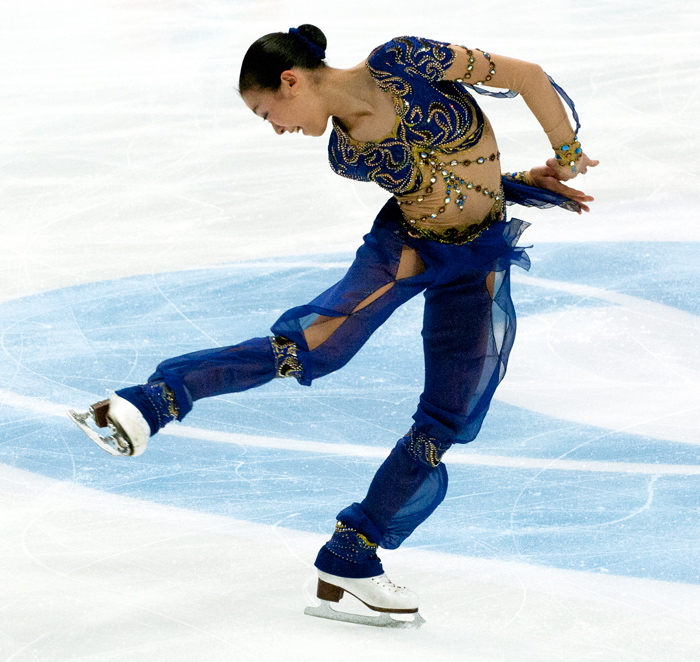
\includegraphics[width=10cm]{Spin/asada.jpg}
\caption{日本花样滑冰选手:浅田真央。}
%\label{default}
\end{center}
\end{figure}

\subsubsection{静止的陀螺}

首先先让我们由一个静止的陀螺开始:

陀螺一头大、一头小,小的一端非常尖,如果我们能够,仅仅是假设让物体的重力通过尖端的话,陀螺即便静止也能够立在支撑点P上。

但这个平衡是不稳定的,我们可以设想桌子的晃动,甚至人的呼吸都能扰动静止的陀螺,使其偏离平衡,然后重力就会使陀螺倒下。但严格说不是重力使陀螺倒下,因为支撑力是能够和重力抗衡的,使陀螺倒下的是力矩,支撑力向上,重力向下,而两个力现在又对不上,这就像两手转动方向盘,向相反的方向用力,总的效果就是方向盘转动起来了。当然这个运动无法持久,陀螺轰然倒地,就像推倒一个立起来的条石。

\begin{figure}[htbp]
\begin{center}
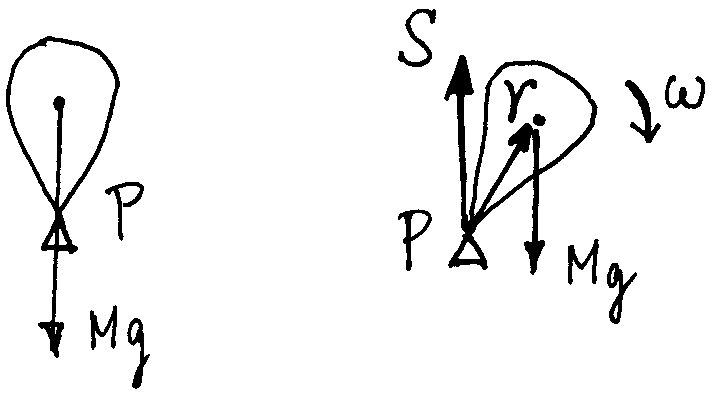
\includegraphics[width=8cm]{Spin/afallingspin.png}
\caption{静止的陀螺会倒下}
%\label{default}
\end{center}
\end{figure}

这种不稳定是很常见的现象,我们把它看作是正常的,是符合直觉的。比如一块立起来的条石,我们轻轻一推它就会倒。

但人呢?从形状上说人接近条石,照道理也是一推就倒,但推倒人要比推倒条石难,因为人是有“灵魂”的,他会根据推力调整自己身体的姿态,人是不太容易被推倒的,但原则上我们加大力,还是可以做到的。

\subsubsection{旋转起来的陀螺}

现在我们让陀螺围绕自身的轴转动起来。其实我们一般讲陀螺的运动,指的都是转动起来的陀螺,而且陀螺本身应该是具有轴对称性的,即陀螺围绕对称轴转动任何角度,在我们看来是一样的。

\begin{figure}[htbp]
\begin{center}
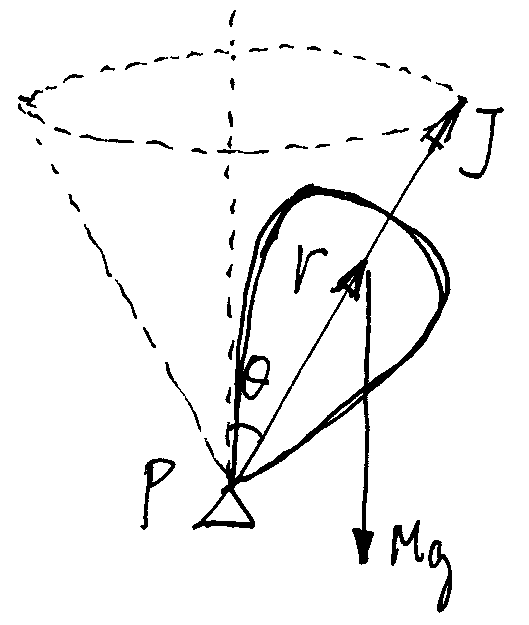
\includegraphics[width=5cm]{Spin/spinningtorque.png}
\caption{旋转起来的陀螺}
%\label{default}
\end{center}
\end{figure}

一个旋转起来的陀螺就是稳定的了,它可以稳定地立在它的尖端。假如我们稍稍偏转陀螺的转轴,陀螺并不会倒下去,它会倔强地以一个稍稍偏离垂直于地面的轴线继续旋转。

~

“陀螺的运动”对我们来说大有象征意义。

首先这是一个违反我们直觉的运动,在我们的直觉中一个歪着的物体,并且是大头朝上,小头朝下,仅凭一个点P与桌面接触,它就应该是不稳定的,它应该与万物一样有向下的趋势。但它偏不!

正因为陀螺行为的反常,所以它才显得好玩,甚至是由灵性的,或接近于神圣的。

在古希腊的观念里,诸天是最神圣的,它们最完美,最善,而最完美最善的几何形体就是“球”。这是爱利亚学派巴门尼德的观念,翻译成现代语言就是球具有最多的对称操作的数目(所谓对称就是某个操作下的不变性,球在任意围绕球心的转动操作下都是不变的),因此它是最完善的。

巴门尼德说的其实不是球,它说的是围绕固定轴旋转起来的球,即天文学意义下的“诸天”。我们现在就知道为什么陀螺是神圣的了,因为它是对神圣诸天的模仿,但它在现实中,在万物皆会腐朽变化的地界,因此它终将会停止旋转,屈服于必朽物向下的趋势,因为各种阻力,各种不够理想的原因。

陀螺是能模仿诸天运行的物件,而且就在我们的身边,可以随身携带,放在兜里面。于是我们看到在电影《盗梦空间》中,梦和现实的区分也是依靠一个旋转的陀螺。梦境是理想的世界,那里的陀螺永不倾倒。而在现实世界里,不论陀螺转的多快,终有倒下的一刻,即人的灵魂、人的意志终有抵挡不住朽坏和变化的那一刻。

\begin{figure}[htbp]
\begin{center}
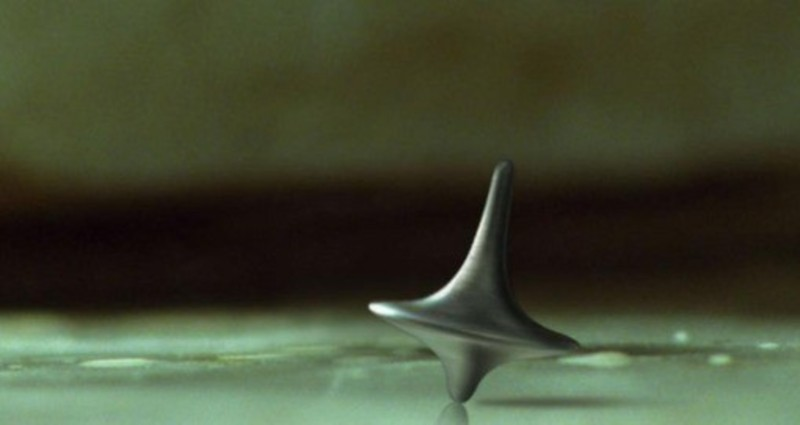
\includegraphics[width=8cm]{Spin/spinningtop.jpg}
\caption{盗梦空间里的陀螺}
%\label{default}
\end{center}
\end{figure}

\subsubsection{陀螺的进动}


旋转起来的陀螺,一般而言会参与两个运动,一个是陀螺自身围绕其对称轴的高速转动,这种转动可以被说成是自己围绕自己的旋转,它看起来是不动的,因此也就有柏拉图在《理想国》第四卷中的著名段落。

\begin{figure}[htbp]
\begin{center}
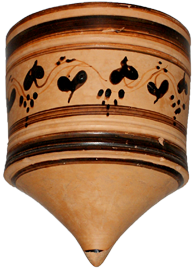
\includegraphics[width=8cm]{Spin/ivyleavestop.png}
\caption{出土于底比斯(Thebes)的公元前5世纪的陀螺,陀螺上装饰有常青藤叶图案。陀螺是当时妇女、儿童喜爱的玩具,同时也是向神献祭的贡品。在观念上旋转的陀螺是对神圣诸天的模仿。}
%\label{default}
\end{center}
\end{figure}


柏拉图说“我们不能讲陀螺既是动的,又是不动的”这种不合逻辑的话,(字面上看这和“波粒二像性”很像)。要说就要说明白,柏拉图采用的方案是“分类”,即把陀螺的运动——这一完整的运动——分解为轴线部分和非轴线部分,他说陀螺的轴线部分——假设陀螺的轴线垂直于地面——是静止的,而陀螺的非直线部分在运动,在三维空间中运动。

更严谨的讨论是:假设陀螺的运动是定点转动,对“陀螺的支撑点”,和“陀螺的非支撑点”分别讨论其运动,陀螺的支撑点是定点因此是不动的,而陀螺的非支撑点部分则是动的。

陀螺除参与围绕自身对称轴的转动外,陀螺整体还会围绕垂直于地面的轴线转动,这个运动和陀螺本身围绕其对称轴的运动不是一个运动,我们一般称之为进动。

即陀螺一边围绕自己转,一边其整体围绕着垂直于地面的轴线转动。陀螺与地面的非垂直的夹角$\theta$会给陀螺一个力矩,这个力矩正好驱动陀螺围绕垂直于地面的轴进动。

在我看来这些运动都是很难想象的,以上是对现象的描述,而要理解这个现象借助于力矩、角动量等自然很简单,但要能够想象这种运动并不容易,这就是我说的反直觉。

陀螺所受力矩是:

\begin{equation}
\tau = Mg r \sin \theta
\end{equation}

假设经过了$\Delta t$时间,陀螺围绕自身轴线高速旋转具有角动量$J$,角动量$J$会以某个角频率$\Omega$围绕垂直于地面的轴线进动。

$\Delta t$时间内,角动量的改变是:

\begin{equation}
\Delta J = J \sin \theta \Omega \Delta t
\end{equation}

最后“力矩乘以时间 = 角动量的改变”,即:

\begin{equation}
\tau \Delta t = \Delta J
\end{equation}

我们可以求出陀螺进动的频率:

\begin{equation}
\Omega = \frac{Mg r}{J}
\end{equation}

我们的结论是,如果陀螺转的越快的话,角动量$J$也就越大,相应地进动频率会比较小。

陀螺是一种反直觉的运动,所谓“反直觉”就是和我们的“想当然”的猜测正好相反。这些都与“旋转”有关,如果翻检物理学史的话,我们能找到不少这样的例子。

\begin{enumerate}
\item 

围绕不同转轴的转动没法交换次序。比如我们先围绕$x$轴旋转$90^o$,然后围绕$y$轴转动$90^o$这一系列的旋转操作和先围绕$y$轴转动$90^o$再围绕$x$轴旋转$90^o$是不一样的。(我们约定所有转动都是逆时针转动)

写成代数式子就是:

\begin{equation}
R_y (\pi /2)  R_x (\pi/2)  \neq  R_x (\pi/2)  R_y (\pi /2)
\end{equation}

这就导致了非对易代数。(其实就是把转动这种操作对应到一种数学语言/结构中去)

\item 

福科摆,假设地球不围绕自己旋转的话,我们是观察不到单摆轨迹的花样的。

\item

电子的托马斯进动。

\end{enumerate}

\subsubsection{惯性导航}

陀螺有一些变种,比如旋转的子弹,它一旦旋转起来,就不会因风等因素使子弹翻转,而保持大致固定的取向。(用物理的语言说就是,假如物体有个大角动量的话,你要改变它的取向$\theta$,你就需要给它一个足够大的力矩。)

\begin{figure}[htbp]
\begin{center}
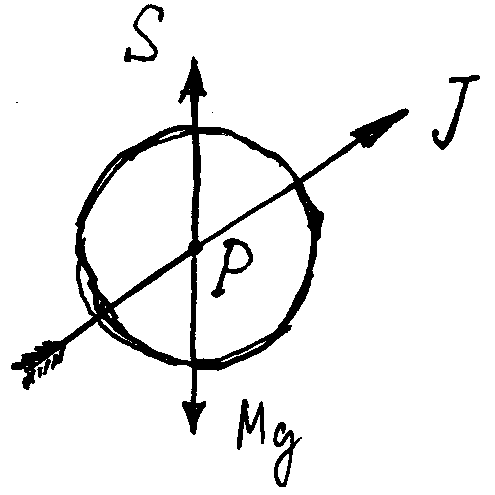
\includegraphics[width=5cm]{Spin/rotationofaball.png}
\caption{陀螺仪原理}
%\label{default}
\end{center}
\end{figure}

可以设想一个飞速旋转的均匀球体,我们假想在球的重心处施加一个向上的力,或我们在想象中把支点固定在球的球心处,所谓支点有两方面的作用,一是支撑,一是固定使其可以被我们带着走来走去。

现在所有的力都是通过支点施加给球的,除此之外它将不受任何外力,因此没有任何力矩会施加在这个球上,因此球的角动量将保持不变。大小和方向都不变,换句话说球的取向将永远不变,不管支点如何动的热闹。

这就是惯性导航的原理,如果我们让这个球高速转起来,并让它的转轴指向某个方向,这个方向将和我们如何运动支点P无关,它永远指向那个固定方向。在此意义下我们的陀螺确实是对神圣诸天的模仿,我们天球的转轴大致是指向北极星方向的。

当然地球并不是一个理想的陀螺,因为它本身的质量分布并不完全对称,这导致了力矩不能完全为0,这导致了地球转轴的方向其实有进动。

这个效应非常小。天文学上叫岁差,一个中等长度的周期是25868年,相比于人生百年,这个变化实在太小了,完全可以忽略。

人类其实很早就发现岁差了,古希腊的天文学家喜帕恰斯(约前190年-前120年)是一个毫不逊色于第谷的古代天文学家,他在比较了他的数据和古巴比伦人的数据后发现了岁差,这再次提示我们科学是一项超越个人生死的集体的事业,若无共同的信仰,持续的观测,岁差或地球自转的进动就不可能被观测到。知识的进步则更加无从谈起。

~

不使用数学,陀螺是一种很难被想象的运动,这一方面使陀螺成为人们好奇的对象,从而成为大人、小孩玩耍的玩具,同时陀螺也保有了一份神秘,就像我们面对星空时的感觉一样,一方面她(现象)是向我们敞开的,我们为之吸引,研究她接近她,但另一方面她又是向我们封闭的,永远向我们保留一部分秘密,提醒我们天与地、永恒与必朽、我与物的区别。(这符合古希腊哲学中对知识、对智慧的定义,我们可以接近她,有认识她的能力,但我们永远处在饥渴和追求的过程中,成为神或全知全能的可能性对人来说是封闭的。)

\begin{figure}[htbp]
\begin{center}
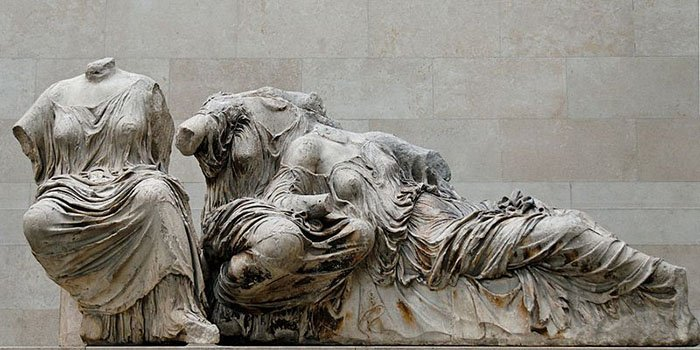
\includegraphics[width=10cm]{Spin/threegoddess.jpg}
\caption{命运三女神雕像:一个女神转动纺轮纺线,一个女神丈量线的长度,一个女神剪短绳子。纺轮的运动也是一种自己围绕自己的转动。}
%\label{default}
\end{center}
\end{figure}

我们现在不知道陀螺是受何种“机械”启发的,纺轮很可能启发了陀螺的发明。或者说纺轮的对象化,去功能化就是陀螺,即陀螺是废弃的纺轮,成为妇女和小孩纯粹娱乐/玩耍的对象。柏拉图在《理想国》第十卷中曾提到过一个关于宇宙的模型,就是基于纺轮、纺杆和挂钩的图像。

\begin{figure}[htbp]
\begin{center}
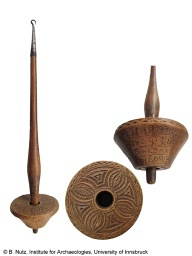
\includegraphics[width=5cm]{Spin/thespindle.jpg}
\caption{古希腊的纺轮、纺杆和挂钩。}
%\label{default}
\end{center}
\end{figure}

\subsection{电子的发现}

电现象是很古老的一种现象。毛皮摩擦橡胶棒带的是负电,玻璃摩擦丝绸带的是正电。我们可以通过接触的方法把电“接”到纸屑上做实验,发现同性相斥,异性相吸,我们还可以把电接到“量电器”上,量电器有两个脚,两个脚因解除都带同性的电,电越多,两个脚的夹角就越大。

关于电的最早的模型是“双流体模型”,所谓流体就是水流,水流可以流来流去,电也可以流来流去,正电和负电分别对应两种流体。但从哲学上假设两种实体是让人不舒服的,比如奥古斯丁就否定有恶的实体,他把恶解释为善的缺乏,或说只有善一种实体。受这种思想的影响,有人就提出单流体模型,把负电解释为正电的缺乏……

当然我们现在知道,有两种电荷,一种是正电,一种是负电……但这种把“负”解释为“正”的缺乏的idea后来在物理里还真用上了,比如狄拉克的“空穴”(hole)概念,所有“负能量”的电子的态都是填充满的,假如我们湮灭掉一个具有“负能量”的电子,就相当于产生了“正能量”的“空穴”,在充满“负能量”电子的背景上,并且电荷是亏空$-e$的,或换句话说我们可以把“空穴”看做是个带相反电荷$e$的正电子,电子的反粒子。

~

现在我们回到对电现象的讨论,牛顿的万有引力定律后,受此启发,大家猜想对电现象应该也有这么一个平方反比的定律,即力的大小正比于距离的平方分之一($F \propto r^{-2}$),两电荷离得越近力越强,越远力越弱。平方反比规律是很直观的,假如我们的空间是三维的,假如我们的质点、电荷会向空间的各个方向放出力线,或散发出某种神秘的“诱惑”,这个力线或诱惑是不应该无缘无故地消失的,它们同时向空间的所有方向跑,假如距离质点或电荷$r$地方我们做一个球面截住这些力线,在这个距离上我们能感受到相互作用的强弱应该正比于力线的密度,即单位面积里力线的“根数”,力线的根数和电荷或质量有关(或更直观地说一个电子或一个质量子放出一根“力线”),而单位面积就是要除以这个同心球面的面积($4 \pi r^2$),力线的密度就是场的强度,假如我们在这个地方再放上另外一个电荷,力的大小就是:

\begin{quote}
场的强度乘以电荷,
\end{quote}

完整写出来:$F \propto \frac{q_1 q_2}{r^2}$。这个力就是库伦力,因为库伦最早做了这个实验,并把比例系数定下来……写成国际单位制就是:

\begin{equation}
F = \frac{1}{4 \pi \epsilon_0 } \frac{q_1 q_2}{r^2}
\end{equation}

这里$\epsilon_0 = 8.854 \times 10^{-12} F/m$,是真空介电常数(Vacuum permittivity)。

~

在原子论的观念下,人们自然会猜测对电现象而言有电的原子。即存在着很小很小的带电的基本单元,甚至我们会把这个基本单元想象为一个小圆球,很多小圆球在一起,看起来就像是一种流体,或用现代的概念讲就是一种“颗粒流”。

在牛顿力学之后,人们有一种对世界的想象,或一种关于世界的整体图景,在这个图景下,世界就是一个质点系统,很多很多质点,质点间有相互作用,在某一刹那($t = t_0 $ ),每个质点的位置和速度(或动量)都是确定的,这时我们就面对一个巨大的联立方程,对每一个质点都是个牛顿第二定律,比如对第$i$个质点:

\begin{equation}
F_i = \sum\limits_{ j \neq i } F_{ij}    =  m a_i
\end{equation}

$F_{ij}$表示第$j$个质点给第$i$个质点的力。但这里力是什么?即质点和质点的相互作用是什么?如果从前的话就是万有引力定律,但现在又多了库伦力,库伦力不同于万有引力的是,第一它可能是吸引的也可能是排斥的,而引力就只能是吸引的,单纯靠引力,世界是不稳定的。第二电磁相互作用,或这里就是库仑力,比引力要强的多,光靠引力我们甚至解释不了最简单的物质——比如氢原子——的结构,但有电磁相互作用就可以。

我们知道有四种相互作用,或三种,引力最弱,强相互作用最强,但它仅存在于原子核里面,剩下的就是“电磁相互作用+弱相互作用”(统称“电弱”,用一套理论描述),我们所处的这个层次的世界,比如为什么会有生命等等,主要是用电磁相互作用解释的。

传统上讲,化学是研究物质结构的。在电化学实验中,我们可以电解水,电解盐酸……

\begin{eqnarray*}
2 H_2 O & \to & 2 H_2 \uparrow + O_2 \uparrow  \\
2 H Cl & \to &  H_2 \uparrow + Cl_2 \uparrow
\end{eqnarray*}

在这些实验中我们会发现产生单位质量的氢气(比如2克)总和确定量的氧气(8克)和确定量的电量转移(1F)相匹配。这提示我们电很可能存在一个最小单元,这个最小单元参与化学反应,它使比如两个氢离子变成一个氢气分子($2 H^+ + 2 e \to H_2  \uparrow $)。并且这个基本单元普遍存在于很多物质中。

~

在发现电子的过程中,塞曼效应(Zeeman effect)是很关键的。所谓塞曼效应就是研究磁场对光的影响,这是法拉第(Faraday,1791 — 1867)临终时研究的课题,但由于他当时用的磁铁不够强大,他没看到磁场对光的任何影响。

法拉第一生做了很多实验,记了好多实验笔记,他的工作奠定了电磁场理论的实验基础。麦克斯韦是电磁理论的数学形式的完成者,所谓场就是物理量(这里就是电场强度$E$/磁场强度$B$)在空间中的分布和时间上的变化,电场和磁场必须看做是个整体,而电场/磁场本身又是矢量,在三维空间上有分量,可以想象电磁场的理论是很复杂的。

麦克斯韦的理论证明光其实就是一种电磁波,一种肉眼可以看见的电磁波,光波波长正好对应太阳——我们的母星——发出的主要电磁辐射。这不是巧合,我们的母星以黄光照亮我们的世界,我们人类的视觉器官也主要适应这个波长,并在这个波长附近进化出辨认不同波长的能力——通过颜色——赤橙黄绿青蓝紫。颜色使我们一眼就能从环境获得更丰富的信息,进而通过生活造就我们内在的心理和智力世界,眼睛充分利用了太阳给我们的馈赠,发达的视觉是人类演化出智慧的基础。

~

牛顿用三棱镜可以把不同波长的光分开,这就是最原始的光谱(spectrum),所谓谱就是分布,光谱就是光强随不同波长的分布($I_{\lambda}$),但牛顿的方法分辨本领不高。

更好的——把不同波长的光分开的方法——是利用光的干涉现象,假如有两束光它们都是从A出发走不同路径,最后都落在屏上的B,如果它们走过的路正好相差波长$\lambda$的整数倍的话,它们就会波峰和波峰叠加,对应光的加强,即一个明亮的条纹,换句话说条纹的位置会和波长的长度有关,不同波长的光会在屏的不同位置出现加强(他强你不强,你不强他强)。现在的问题是要让条纹们变窄一点,否则都叠在一起不好测量。

我们可以使用光栅来使条纹变窄,所谓光栅就是把光分成细而密集的很多束,比如最早的光栅就是用金属丝缠绕而成的,而晶体因为本身就有周期性结构,可以看做是天然的光栅。

假设有很多束光,它们两两之间正好相差$\delta$相位$e^{i \delta}$,所有这些波的叠加是:

\begin{equation}
1 + e^{i \delta} + e^{i 2 \delta } + ... + e^{i N \delta}
\end{equation}

这是一个等比数列,我们可以求出和是:

\begin{equation}
\frac{1 - e^{i N \delta}}{ 1 - e^{i \delta}} = \frac{ 1- \cos N \delta - i \sin N \delta }{ 1- \cos \delta - i \sin \delta}
\end{equation}

光强正比于波幅的绝对值的平方:

\begin{equation}
I(\delta) \propto \frac{( 1 - \cos N \delta)^2 + \sin^2 N \delta  }{  (1 - \cos \delta)^2 + \sin^2 \delta } = ... = \frac{\sin^2 N\delta /2}{\sin^2 \delta /2} 
\end{equation}

可见增加$N$会有效地提高光栅的分辨本领,随着光栅技术的进步,我们能够把不同波长的光在光谱上分的越来越开。

~

与此同时洛伦兹基于麦克斯韦的电磁场理论提出了他的关于金属的理论,他假设金属里面有很多带电的基本粒子,它们和分子运动论中讨论的原子一样在做无规则的热运动,在这样一幅图像下洛伦兹解释了电的输运现象,比如为什么会有欧姆定律(Ohm's law)。

塞曼是洛伦兹的助手,他受法拉第想法的启发,想再试一试磁场对光的影响,当时实验技术已经有很大进步了,更大的磁铁,更精细的对光波波长的分辨等等。塞曼对磁场中的钠光谱进行了分析,发现磁场能够使钠的黄线变粗(就是分裂了),他测量了波长的变化,并把结果告知洛伦兹。

洛伦兹很快基于他的电子论给出了对塞曼效应的解释。假设金属里面有带电的基本单元,这个基本单元的运动对物性负责,现在磁场加上去了,就有洛伦兹力$q v B$,洛伦兹力是有方向的,假设带电粒子既可以围绕磁场顺时针转动,也可以逆时针转动,这个力对顺时针转动和逆时针转动的影响就是相反的,它使得一个转动变快,而使另一个转动变慢。转动快慢对应频率,而频率对应波长。

\begin{equation}
\lambda = c T = \frac{c }{\nu} = \frac{2 \pi c}{ \omega }
\end{equation}

洛伦兹基于以上思路做了一个简单的计算,正好可以解释塞曼的实验结果。并且给出了一个重要的结果,假如金属中的这个带电单元既有质量($m$)又有电荷($q$)的话,它们的比值将是$q/m \propto 10^{11} $库伦/千克。

几个月后,JJ汤姆逊就对阴极射线完成了他的著名实验,在这个实验中他对阴极射线的轨迹进行了直接的测量,阴极射线在磁场的作用(洛伦兹力)下会偏转,这用粒子图像很容易解释。汤姆逊测出了阴极射线的电荷质量比,也是大约$10^{11}$库伦千克。

关于存在电的基本单元,我们现在就有了好几个独立的证据,电解实验表明在水、盐酸……中存在着带电的基本单元,塞曼效应说明在金属中存在带电的基本单元,汤姆逊实验说明在阴极射线里有带电的基本单元,而且我们还观察到了带电基本单元在磁场和电场下的偏转,这可以说是更直接的证据。

现在汤姆逊就假设在物质中普遍存在带电的基本单元,并称之为电子,它是负的,电荷质量比是$10^{11}$库伦/千克量级。汤姆逊还猜测,如果存在带正电的基本单元的话,其电量应该和带负电的基本单元——电子——相同,只是正负号相反。这个猜测是合理的,因为在电解水实验里就是电子在离子之间跑来跑去,这意味着一个氢离子(质子)加一个电子正好就是电中性的。

\begin{eqnarray*}
2 O^{--} & \to &  O_2 \uparrow + 4 e \\
4 H^+ + 4 e  & \to & 2 H_2 \uparrow 
\end{eqnarray*}

我们也可以用磁场偏转质子来测量质子的电荷质量比$e/m_p$,发现这个数比电子的电荷质量比小很多,说明电子比质子轻很多。这个结果让我们很不舒服,因为自然界中带负电的基本单位竟然比带正电的基本单位轻很多……假如质量一样,只是电荷相反我们就会觉得舒服,有“左右对称”式的“均衡”感。现在我们知道有电子有反电子,有质子也有反质子,这就舒服多了,于是问题就变成为什么我们的这个世界电子会比反电子多很多……,这个问题是被苏联物理学家萨哈罗夫解决的。

密立根通过油滴实验测出电子电荷的具体数值$e = 1.602 \times 10^{-19} C$,这意味着现在电子的质量也知道了$m_e = 9.109 \times 10^{-31} kg$。

那么电子有多大呢?我们现在有两个简单的选择,一种是把电子想象为一个球体,它的半径是$r_e$,电荷和质量都均匀地分布在这个球体上。另一种选择是把电子干脆看成是一个点,好比曾经的质点模型,我们用位置和速度描述电子的运动状态(或在量子力学中,以位置和时间为变量的波函数$\psi(x,t)$),就电子本身而言,它的质量是$m_e$,电荷是$e$(虽然说电子带负电,但我们还是习惯把它写为$e$,这里的逻辑很简单,就是省事)。

~

回到塞曼效应,进一步的实验表明,塞曼效应比我们想象的复杂,我们可以把不同的金属放进磁场里,测不同的谱线分裂。我们发现谱线可能会分裂成偶数条,这是洛伦兹粗糙的电子论无法解释的。我们把理论上好解释的叫“正常塞曼效应”,把暂时还没法解释的起名叫“反常塞曼效应”。但实际上大部分观察到的是“反常塞曼效应”,或者说你们“正常”的其实才是“反常”的。

塞曼效应(磁场中光谱线的分裂)是原子物理中的一个重要实验,因为它很早就发现了,一直没获得完满的解释,或者说它一直在驱动理论演进。此外塞曼效应还启发人们去研究电场中光谱线的分裂,这就是斯塔克效应(Stark effect),斯塔克效应对催生量子力学也有重要作用。

~

根据物质的摩尔质量,密度等参数我们可以估计不同元素原子的大小,其结果非常整齐,都是$10^{-10}$米,即不管它们的密度多么悬殊,但对于构成它们基本单元的原子,不同种类原子的大小是差不多的。

\begin{table}[htdp]
\begin{center}
\caption{不同原子的半径}
\begin{tabular}{|c|c|c|c|}
\hline 
元素&   质量数$A$&    质量密度$\rho$($g / cm^3$)&
原子半径($nm$)\\
\hline
Li &  7&  0.7&   0.16\\
Al & 27& 2.7& 0.16\\
S &  32& 2.07&    0.18\\
Cu &  63& 8.9&    0.14\\
Pb &  207& 11.34&    0.19\\
\hline
\end{tabular}
\end{center}
\end{table}

我们还可以估计电子的大小$r_e$,根据狭义相对论,质量就是能量,能量就是质量,电子的质量$m_e$对应能量$m_e c^2$,而电子本身还带电荷$e$,电荷周围是电场的分布,假设电荷是个半径为$r_e$的均匀带电球体的话,我们能把电场在整个空间的分布$E(r) $都计算出来,根据电磁学,电场是有能量的,单位体积的能量(或能量密度)是$ \frac{\epsilon_0}{2} E(x)^2$,我们把所有电场的能量都加起来,它将是一个和参数$r_e$有关的表达式,这样表达出的能量要和电子的总能量$m_e c^2$相等。相当于我们从两个角度计量了电子的总能量,然后我们就能计算出$r_e$。

这样计算出来的$r_e$很小,大约是$10^{-15}$米,它比原子的尺度$10^{-10}$米小很多,就相当于我们在足球场里爬进了一只小蚂蚁。

这个计算很微妙,首先它似乎否定了电子——是个几何点——这样的物理图像(因为这样的话总能量会趋于无穷大),其次它是通过考虑相对论来否定的。这意味着我们必须考虑相对论才能得到一个关于电子的完整理论。这也是当时物理学家的普遍想法,因为狭义相对论1905年就提出了,把所有物理理论推广使其符合相对论是当时很多理论家喜欢做的事情。

我们还知道电子不是经典的对象,我们必须发展量子力学的理论才能描述它的运动,假如电子的运动速度很慢,也许存在一个非相对论性的量子力学,但如果电子的运动速度接近光速,就必须使用相对论性的量子力学。

当时很多物理学家都希望能直接得到一个关于电子的相对论性理论,但最后都失败了。首先成功的还是一个关于电子的非相对论性理论,即海森堡-玻恩-约丹的矩阵力学和薛定谔的波动力学。

\begin{figure}[htbp]
\begin{center}
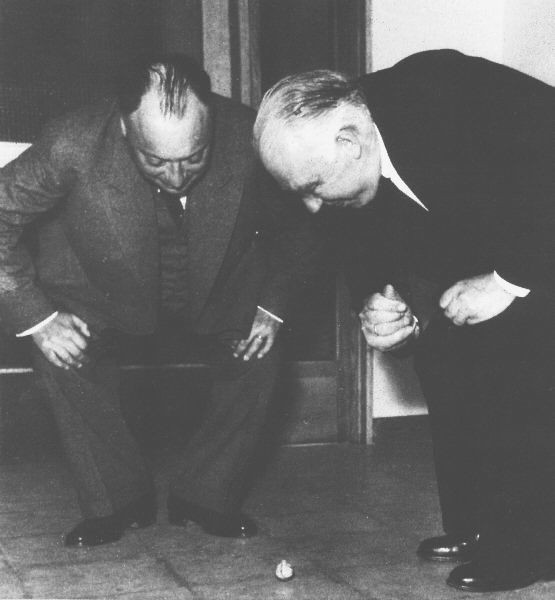
\includegraphics[width=6cm]{Spin/bohrandpauli.jpg}
\caption{玻尔和泡利在一起玩陀螺。}
%\label{default}
\end{center}
\end{figure}

在非相对论性量子力学中,电子是被当做点处理的,因为把电子处理为球体,并认为电子会像地球一样自转起来恰恰无法解释反常塞曼效应。我们必须接受这样一个尴尬的局面——我们把电子理解为点,但同时这个点还必须能有角动量(自旋角动量$s$)和磁矩。这是非常别扭的,我们在经典物理中根本就找不到这样的例子\footnote{这是柏拉图在《理想国》第四卷中讨论的问题,对于一个点我们能说它围绕自身旋转吗?

柏拉图否定了点能旋转,用我们今天的话说就是“对于一个几何的点,没有自转,只能是静止的”。

那什么是转动呢?

如果我们把转动定义为物体的一部分相对于另一部分在空间中的运动的话,我们就可以立刻说对于点是不可能有自转的,因为它没有部分(点在《几何原本》中的定义是“没有部分”)。

更多请参考:“柏拉图、陀螺和自旋”, \url{http://jianshu.io/p/3f98e4086955} }。

如果我们回顾海森堡等创建量子力学的过程的话,他们非常依赖于把原子现象(量子力学)与日常经验(经典力学)进行类比,他们建立了一整套对应的法则,根据这些法则,我们由经典力学的概念、公式出发就会得到相应量子力学的概念、公式。比如经典力学中的位置$r$对应量子力学中的位置算符$\hat r$;经典力学中的角动量$L$对应量子力学中的角动量算符$\hat L$;经典力学中的泊松括号对应量子力学中的对易关系等等。

这里我们碰到的就是这个困难——自旋角动量$S$没有经典对应,它是个纯粹的量子现象,我们没法用一个陀螺的旋转(或任何其他经典现象)与之对应。

这个困难必须到狄拉克的相对论性量子力学才能得到解释,在那里电子仍然被当做一个点来处理,但这个点所满足的运动方程是个矩阵方程,它可以求出四个解,两个解是正能量,两个解是负能量。负能量解对应的是反电子(为了好理解,狄拉克把它解释为电子背景上的空位,即空穴,但到量子场论里我们是不需要借助这个图像的),而两个解分别对应自旋向上和自旋向下。电子和反电子在形式上现在就对称了,它们质量相同,什么都一样,就是电荷不同。

现在我们再来说电子的话,电子就是这样一个对象,它的自旋角动量是1/2,质量是$m_e$,电荷是$e$,电子本身的运动状态要用波函数来表示,但有两个分量,一个对应自旋向上,另一个对应自旋向下。我们可以把它写为列向量的形式:

\begin{equation}
\left(  
\begin{array}{lcr} 
\psi_{s \uparrow} \\
\psi_{s \downarrow}
\end{array}
\right)
\end{equation}


\subsection{自旋的发现}


有两种讲授量子力学的方法,一种是按照历史的逻辑,介绍黑体辐射、关电效应、康普顿散射、卢瑟福散射、玻尔模型、塞曼效应等一系列著名实验,说明经典物理是如何失效的,然后建立“波粒二像性”概念,即“像波一样的粒子”,然后我们用波函数、薛定谔方程来描述电子。

以氢原子为例,不考虑相对论,我们需要求解这样一个偏微分方程:

\begin{equation}
i \hbar \frac{\partial }{\partial t} \psi (r, t) = \left[ -\frac{\hbar^2 }{2m} \nabla^2 + V(r) \right] \psi (r, t) 
\end{equation}

还有一种讲授量子力学的方法是直接从某一个实验出发引入量子力学。比如费曼就是从假想的双缝实验出发建立量子力学的,讨论双缝实验的好处是方便和费曼发明的路径积分方法对接。除双缝实验外还有一个选择,就是通过讨论斯特恩-盖拉赫实验引入量子力学。

但首先,让我们讨论“磁矩在磁场中运动”。

\subsubsection{磁矩在磁场中运动}

所谓磁矩就是一个小磁针。假设一个小磁针放到磁场里,磁矩在磁场中不受力,但会受到力矩的作用,它会倾向于倒向和磁场平行的取向。

\begin{figure}[htbp]
\begin{center}
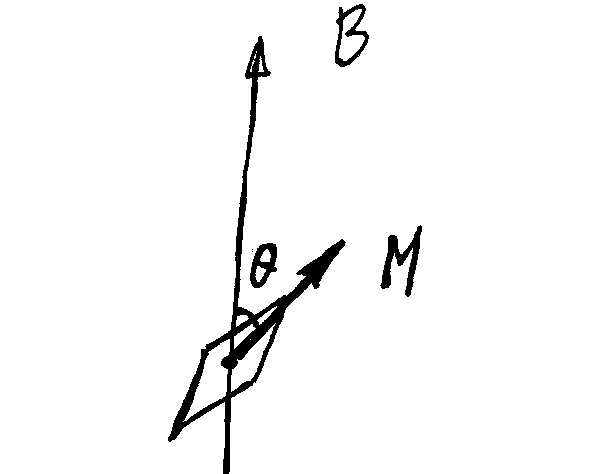
\includegraphics[width=4cm]{Spin/momentinB.png}
\caption{在磁场中的磁矩。}
%\label{default}
\end{center}
\end{figure}

假设磁针的磁矩是$M$,磁场是$B$,其能量为:

\begin{equation}
U = - B \cdot M
\end{equation}

类似于陀螺会在重力场中进动,磁矩也会围绕磁场进动。

力矩是:

\begin{equation}
\tau = \mu \times B = \frac{d J}{d t}
\end{equation}

这里$J$是角动量。

假设这里的磁矩$\mu $、角动量$J $都是“环形电流”导致的,即假设电子围绕$z$轴做圆周运动导致的磁矩和角动量。

\begin{figure}[htbp]
\begin{center}
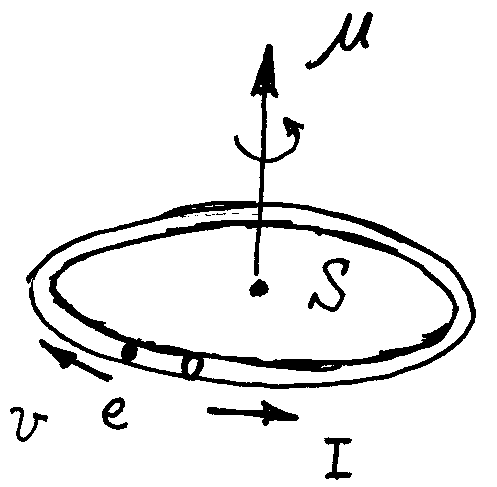
\includegraphics[width=5cm]{Spin/currentrotate.png}
\caption{电子的运动导致环形电流。}
%\label{default}
\end{center}
\end{figure}

角动量:

\begin{equation*}
L = r \times p =  m r^2 \omega 
\end{equation*}

磁矩$\mu$等于电流$I$乘以电流围成的面积$S$,电流是单位时间通过某截面的电荷数,即$I = \frac{\Delta Q}{\Delta t}$,如果取电子运行周期$T$是$\Delta t $的话,$\Delta Q$正好是电子的电量$- e$(负号表示电子带的电量是负的)。

现在:

\begin{eqnarray*}
\mu & = & IS = - \frac{e }{T } \pi r^2 \\
{} &=& - \frac{e}{2m} L
\end{eqnarray*}

换句话说电子的轨道运动会导致电子具有轨道运动的角动量(就像地球围绕太阳运动,地球会具有轨道角动量一样),同时电子是带电的,因此电子的轨道运动也会导致电子具有磁矩,就像一个环形电流会具有磁矩一样,因为都是电子的运动导致的,我们会发现磁矩和角动量是成正比的,我们把这个比例因子进一步改写为:$- g \frac{e}{2m}$,这里负号表示电子是带负电的,$g$是朗德因子,因为我们很快将发现电子不但具有轨道磁矩,它还将具有自旋磁矩。

字面上理解好像是说电子会同时参与两个运动,就像我们的地球在太阳系里的行为一样,一个是电子因轨道运动(这里就是半径为$r$的匀速圆周运动)导致的磁矩,另一个是电子因自旋运动(字面意思就是电子自己围绕自己旋转)导致的磁矩。对轨道运动而言$g_L = 1$,对自旋运动而言$g_S = 2$。写成统一的形式:

\begin{equation}
\mu = - g \frac{e}{2m} J
\end{equation}

我们用$J$表示一般的角动量,用$L$表示轨道角动量,$S$表示自旋角动量,当然马上我们会发现“自旋”(Spin)是个错误的命名。

在原子物理中我们用玻尔磁子(Bohr magneton, $\mu_B$)作为磁矩的单位:

\begin{equation}
\mu_B = \frac{e \hbar }{ 2 m} 
\end{equation}


%但为什么是2呢?

\subsubsection{斯特恩-盖拉赫实验}

我们可以通过讨论斯特恩-盖拉赫实验直接引入量子力学。

斯特恩-盖拉赫实验是个充满了意外的实验,斯特恩(Otto Stern)是爱因斯坦的第一个学生,但他却是个实验物理学家,他想用实验验证当时原子物理研究中的主流理论——“玻尔-索末菲模型”(Bohr-Sommerfeld model)。

玻尔模型是个大杂烩,为了解释原子光谱他把很多并不相容的假设捏在了一起。比如他让电子在一个轨道上围绕原子核运动,这就是经典力学。但他又引入了量子化条件,只允许电子在几个分立的轨道上围绕原子核运动,这就又不要经典力学了。

但既然玻尔模型能够很简单地解释氢原子光谱,而且推导又那么简单,物理学家认为这个对原子现象的描述还是很有潜力的,比如索末菲就对玻尔模型进行了推广。原子中电子和原子核之间符合库伦力,一个平方反比的吸引力,原子核本身的质量比电子质量大很多很多,这些都使得原子就像是一个微小的太阳系,根据开普勒的运动定律行星在一个椭圆轨道上围绕太阳运动,而椭圆是可以有不同偏心率的(圆是一种特殊的椭圆,偏心率为0)。

索末菲把玻尔模型中的圆轨道推广到椭圆轨道,同时他把玻尔的量子化条件也推广了。他引入了两个量子数,一个角量子数$n_\phi$,使:

\begin{equation}
\oint p_\phi d \phi = n_\phi h , n_\phi = 1, 2, ...
\end{equation}

这里$\phi$是电子在椭圆上运动时的方位角,$p_\phi = \frac{\partial L }{\partial \dot \phi }$,$L ( r, \phi; \dot r , \dot \phi  ) = T - V$是拉氏量。

另一个是径向的量子数$n_r$,使:

\begin{equation}
\oint p_r dr = n_r h , n_r = 0, 1, 2, ...
\end{equation}

使用极坐标系($r , \phi$)描述电子在原子核附近的位置,$r$是矢径,从原子核指向电子,$p_r$定义为$\frac{\partial L }{\partial \dot r }$。对正圆运动来说,$r$是个常数,所以$n_r$是可以等于0的。

\begin{figure}[htbp]
\begin{center}
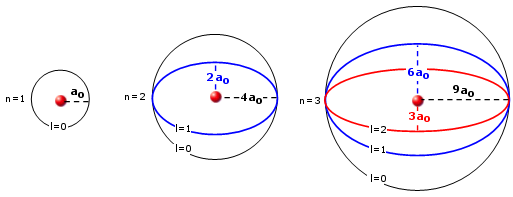
\includegraphics[width=11cm]{Spin/bohr-sommerfeld-model.png}
\caption{玻尔-索末菲模型,这里$l$相当于是$n_r$}
%\label{default}
\end{center}
\end{figure}




$n_r + n_\phi = n $,$n = 1, 2, 3, ...$就是原先玻尔模型中的量子数$n$(主量子数)。

\begin{table}[htdp]
\caption{玻尔-索末菲模型}
\begin{center}
\begin{tabular}{|c|c|c|c|}
\hline
主量子数$n$ & 角量子数$n_{\phi}$ & 磁量子数$m$ & 矢径量子数$n_r$ \\
\hline
1 & 1 & $\pm 1$ & 0 \\
\hline
2 & 2 & $\pm 2$ & 0 \\
{} & 1 & $\pm 1$ & 1 \\
\hline
3 & 3 & $\pm 3$ & 0 \\
{} & 2 & $\pm 2$ & 1 \\
{} & 1 & $\pm 1$ & 2 \\
\hline
\end{tabular}
\end{center}
\label{default}
\end{table}%


对$n = 1$而言,$n_\phi = 1$,$n_r$只能等于0。这是氢原子能量最低的态,称之为基态。考虑到电子既可以是顺时针围绕原子核运动,也可以是逆时针围绕原子核运动的,于是一个$n_\phi$就对应两个“状态”,用角动量的语言说就是$L = \hbar$,但角动量在$z$方向上的投影只能取$L_z = \pm \hbar $两种情况,即角动量的取向也是量子化的,只能沿$z$轴向上或向下。我们把$L_z$写作$m \hbar$,这里$m = \pm 1$,我们管$m$叫做磁量子数,只要$m$不是0,原子就会在$z$方向上有非0的磁矩。


量子化条件会引入不同于经典物理的陈述,比如能量分裂成一个一个能级——能量量子化;现在又导致角动量的$z$分量只能取分立值(对氢原子基态而言是两个),我们称这种现象为空间取向的量子化(Space quantization)。

%对$n=2$而言,$n_\phi = 1, 2$,$n_r = 0, 1$……

虽然“玻尔-索末菲模型”能解释不少物理实验,但对这么一个大杂烩式的理论,物理学家并不真的相信。比如电子是否真的会在原子里面按照圆形或椭圆形的轨道运动?这样的图像辅之以量子化条件等也许能够解释实验,但如果电子真的这么行为的话,那也太神奇了。

\begin{figure}[htbp]
\begin{center}
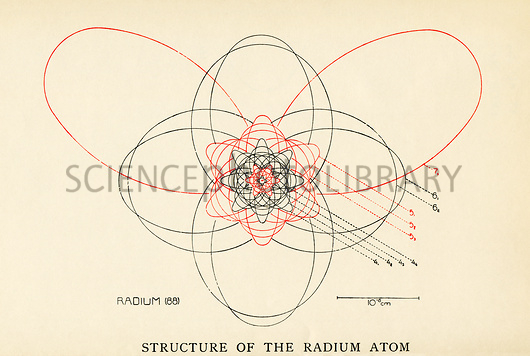
\includegraphics[width=10cm]{Spin/Bohr-Sommerfeld_model_of_the_atom.jpg}
\caption{玻尔-索末菲模型下的“镭”原子}
\label{default}
\end{center}
\end{figure}

斯特恩是物理化学的博士,但他却有幸成了爱因斯坦的第一个学生,作为犹太人,他的父母坚决资助他们的儿子继续深造。一战结束后,斯特恩又成了玻恩的助手,当时玻恩在法兰克福大学任教并领导一个实验室,在那里斯特恩研究了原子束方法。所谓原子束方法就是用一个炉子给金属加热,使金属原子从炉子里跑出来,通过准直装置后,然后再对射出来的金属原子进行各种操作和测量。

斯特恩知道要想验证氢原子的“空间取向量子化”,就要让$L_z = \pm \hbar$的基态氢原子分开,但如何把不同$L_z$的氢原子分开呢?斯特恩有一天醒早了,当时是冬天,他怕冷于是就躺在被窝里想这个问题。他想到可以让氢原子通过一个在$z$方向上的非均匀磁场$B(z)$,磁场的非均匀性可以通过磁场的梯度$\frac{d B(z)}{d z}$来描述,如果梯度足够大的话,就有可能把不同角动量的原子分开。

%%%%

假设原子的磁矩是$\mu$,它在磁场中的能量是:

\begin{equation}
U_m = - \mu \cdot B = \mu_x B_x + \mu_y B_y + \mu_z B_z 
\end{equation}

由于磁场是非均匀的,磁矩将会受到一个非0的力:

\begin{equation}
F = - \left( \hat x \frac{\partial }{\partial x} + \hat y \frac{\partial }{\partial y}  + \hat z \frac{\partial }{\partial z}  \right) U_m  = \hat z  \mu_z  \frac{\partial B_z }{\partial z}
\end{equation}

这里$\hat x $,$\hat y $,$\hat z $分别是$x, y$和$z$方向上的单位矢量,换句话说,原子受到的力在磁场的非均匀方向上,即$z$方向上,力的大小是:

\begin{equation}
F =  \mu_z  \frac{\partial B_z }{\partial z}
\end{equation}

可见这个实验的难点确实在磁铁上,磁铁的规格要使得$\frac{\partial B_z}{\partial z}$越大越好,同时磁铁要足够长,这样不同大小的力会驱动银原子在$z$方向上漂移足够长时间,使具有不同磁矩的原子充分分开。

%%%%

斯特恩有了这个想法后很兴奋,于是跑去向玻恩汇报,但玻恩并不认为这个实验有价值,在他看来“空间取向量子化”无非是个象征,在它的背后还有我们暂时不懂的物理,而斯特恩竟然在字面上相信会有这么回事,……,这就是他自己的事了\footnote{“It took me quite a time before I took this idea seriously. I thought always that (space) quantization was a kind of symbolic expression for something which you don’t understand. But to take this literally like Stern did, this was his own idea… I tried too persuade Stern that there was no sense (in it), but then he told me that it was worth a try.” 摘自:“Stern and Gerlach: How a Bad Cigar Helped Reorient Atomic Physics”,Physics Today 56, December 2003, \url{http://zimp.zju.edu.cn/~xinwan/qm2/note/PhysToday_Friedrich03.pdf}}。

斯特恩获得了盖拉赫的帮助,而盖拉赫直到此时才第一次听说“空间取向量子化”。实验很难做,花了斯特恩和盖拉赫一年多时间。

他们使用的是银原子Ag,用炉子把银加热到1000多摄氏度,然后使跑出来的银原子通过两个只有0.03毫米宽的准直装置。磁铁有3.5厘米长,磁场强度是大约0.1特斯拉,在$z$方向上的梯度达到了10特斯拉每厘米。银原子确实分裂成了两束,两束的间隔只有0.2毫米,而准直装置或磁铁的方位只要差0.01毫米就会把银原子的分裂图样破坏掉。可想而知这是一个十分精细的实验。

\begin{figure}[htbp]
\begin{center}
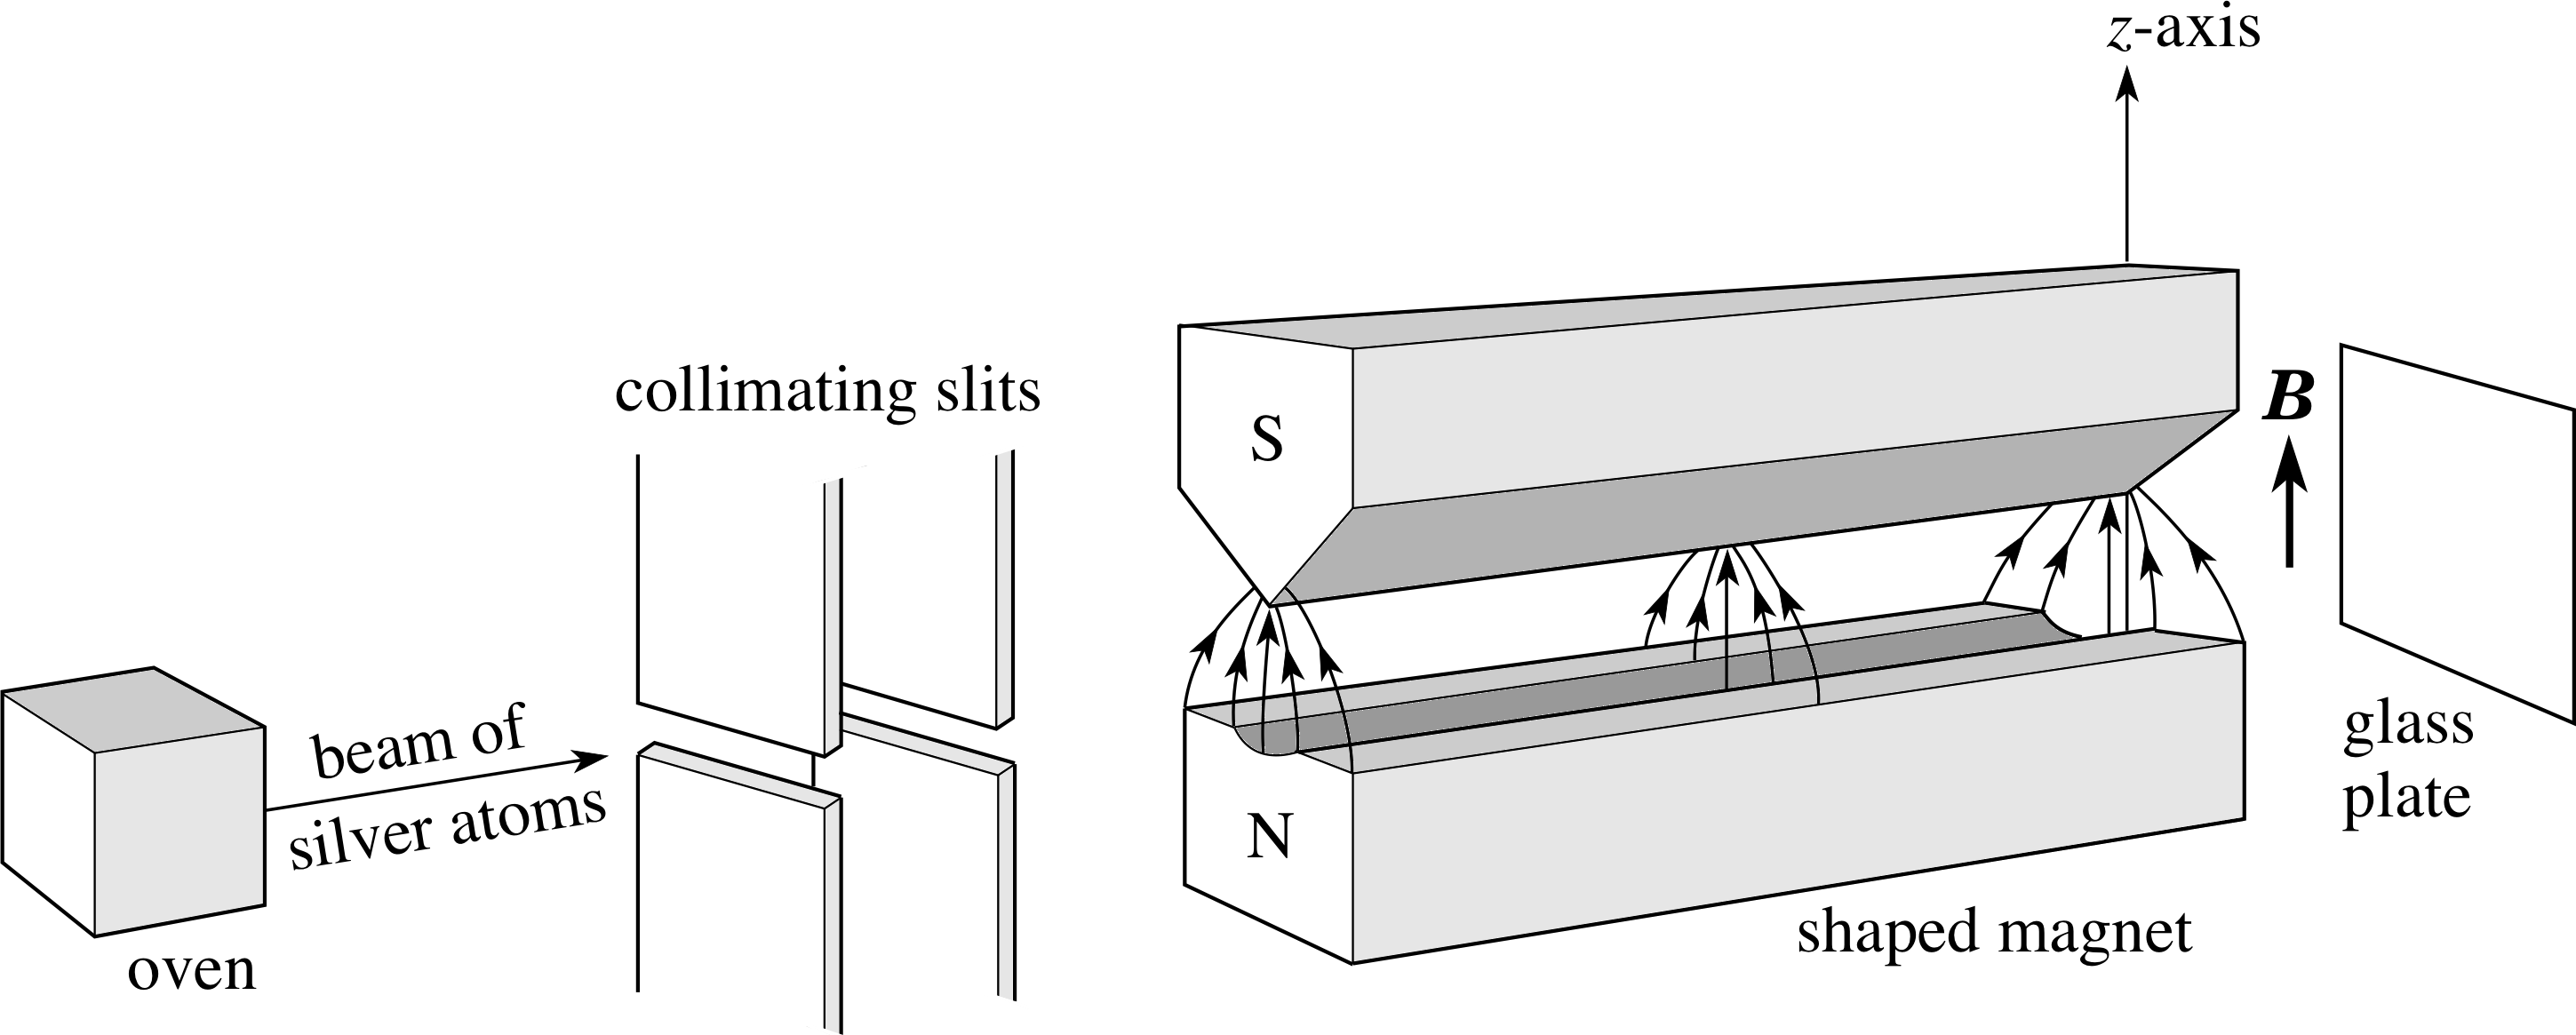
\includegraphics[width=11cm]{Spin/SGexperiment.png}
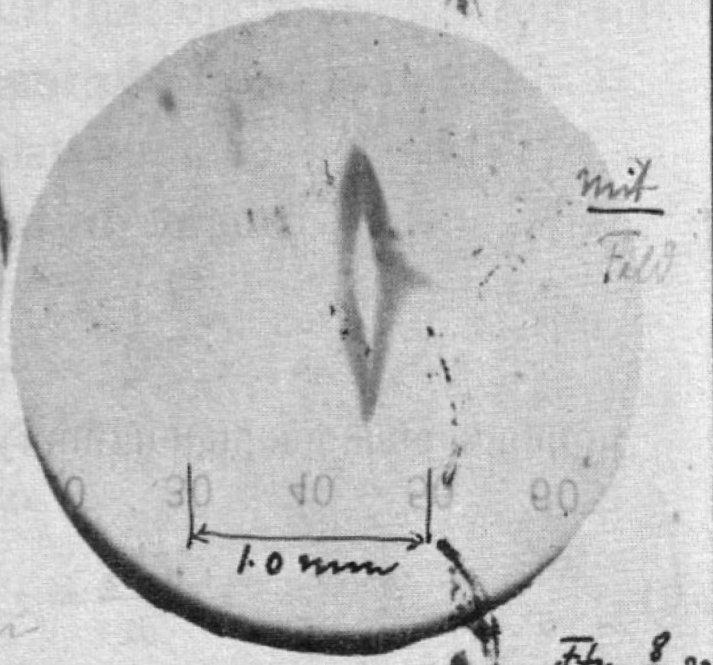
\includegraphics[width=8cm]{Spin/splitting.jpg}
\caption{上:斯特恩-盖拉赫实验装置图。下:最终条纹分裂只有0.2毫米,但很清晰。}
%\label{default}
\end{center}
\end{figure}


积累在靶上的银原子很少,盖拉赫什么都没看到,他把靶板递给斯特恩,这时他们看到银原子积累的痕迹逐渐显现。很神奇,他们把这归结为银的硫化,因为斯特恩当时的薪水很低,他在实验室里抽劣质的雪茄,他们分析可能是劣质雪茄里的硫太多了,使银硫化,而硫化银是黑色的,很容易被看到。

尽管如此,斯特恩和盖拉赫仍然无法得到稳定的图样,他们的结果在证实和否定“空间取向量子化”之间摇摆。同事们也质疑他们的实验,比如德拜就认为“空间取向量子化”根本就不可能被观察到\footnote{“But surely you don’t believe that the (spatial) orientation of atoms is something physically real; that is (only) a timetable for the electrons.”  摘自:“Stern and Gerlach: How a Bad Cigar Helped Reorient Atomic Physics”,Physics Today 56, December 2003, \url{http://zimp.zju.edu.cn/~xinwan/qm2/note/PhysToday_Friedrich03.pdf} }。

斯特恩和盖拉赫都是挺固执的人,面对质疑盖拉赫说:“在这个世界上没有不值得试的事情。”(No experiment is so dumb, that it should not be tried.)

除此之外,他们还碰到很严峻的财务危机,当时德国正处在一战后的困苦中,玻恩竭尽一切办法为斯特恩-盖拉赫实验筹款。他利用公众对相对论的兴趣在学校最大的演讲厅内为爱因斯坦办系列公共演讲,并对参加的听众收取门票。但通货膨胀太厉害了,靠这笔钱也就支持了几个月。最后还是多亏了美国的银行家Goldman(金人)\footnote{Goldman是著名投行Goldman Sachs(高盛)的创始人,他虽然是犹太人但对德国比较友好,1930年代初起移居德国。1936年,在大屠杀发生的前夜,Goldman狼狈逃出德国,保住性命,但其在德财产皆被纳粹没收。}出手寄了几百美元给玻恩。于是,实验继续。

尽管如此,实验进展得仍不如意。1922年,斯特恩去罗斯托克做教授,他和盖拉赫在哥廷根碰头决定放弃实验。但一次铁路罢工改变了这个实验的命运,当时盖拉赫正坐着火车在回法兰克福的途中,因为罢工他在火车上又把实验的种种细节回顾了一遍,他想到了如何改进准直的新主意,回到法兰克福后他继续实验,这一次他获得了非常清晰的分裂条纹。进一步的计算表明,条纹的分裂确实对应$\pm 1$个玻尔磁子($\mu_B $)磁矩的区别,误差在10\%左右。

1922年2月13日,盖拉赫给玻尔寄出一张明信片,背后附有实验结果的照片。明信片上说:“尊敬的玻尔先生:附上我们……所得方向量子化的实验证据。我们祝贺您的理论得到证实。”

表面看这是对玻尔-索末菲理论的直接证实,但其实只是巧合。求解氢原子的薛定谔方程,我们可以得到三个量子数:

\begin{quotation}
主量子数:$n$,$n = 1, 2, ...$

角量子数:$l$,$l = 0, 1, 2, ... n-1$

磁量子数:$m$,$m= 0, \pm 1, \pm 2, \pm l$
\end{quotation}

氢原子的基态,对应$n=1$,$l = 0$,$m = 0$,换句话说氢原子的基态应该是没有角动量的,也没有磁矩。当然斯特恩-盖拉赫实验里用的是银原子,银原子正好只剩一个5s电子在最外层,其他电子在内层,其磁矩都相互抵消掉了。对5s电子而言,$n =5$,$l = 0$,$m = 0$,也没有角动量和磁矩。

那么斯特恩-盖拉赫实验应如何解释呢?实际上它是表明电子具有新角动量——自旋角动量$S$的实验证据。自旋(spin)这个名称来自与经典图像的类别,但这个对比又是不成立的!换句话说这个名字取错了,但名字无非是个指称,物理学家似乎不太在乎这个名字会给门外汉带来误导,他们只是强调自旋是电子(或粒子)的内禀性质,和空间位置($x, y, z$)无关,既然和空间位置无关,我们也就无法把自旋想象成一种在三维空间里发生的自己围绕自己的转动了。

仿照玻恩的句式,我们可以这么说:

\begin{quote}
自旋只是个符号,你要是做字面理解那你可就太Naive了。
\end{quote}

\subsubsection{连续的斯特恩-盖拉赫实验 }

自旋不是真实的,但无论如何斯特恩-盖拉赫实验是真实的。我们可以忘掉玻尔-索末菲理论,继续挖掘这个实验的内涵。

我们把具有$z$方向上的非均匀磁场的斯特恩-盖拉赫装置记做$SGz$,银原子通过$SGz$后将在$z$方向上分裂为两束。分别对应磁矩为$\pm \mu_B$,磁矩是在$z$方向上的,我们称$- \mu_B$的那束为$s_z = \frac{1}{2}\hbar$,$\mu_B$的那束为$s_z = - \frac{1}{2}\hbar$(假设自旋的朗德因子是2,$g_S = 2$,负号很讨厌,这是因为电子带的是负电)。

非均匀磁场的取向是任意的,如果我们设法使银原子通过一个$x$方向非均匀的磁场,即通过SGx,我们会观察到银原子在$x$方向上的分裂,分裂成对称的两束,对应$x$方向上的磁矩$\pm \mu_B$,$- \mu_B $对应的那束是$s_x = \frac{1}{2} \hbar$,$\mu_B $对应的那束是$s_x = - \frac{1}{2} \hbar$。

类似地,我们让银原子通过$y$方向上的非均匀磁场$SGy$,我们会观察到银原子在$y$方向的分裂,也是对称的两束,我们称$- \mu_B$对应的那束是$s_y = \frac{1}{2} \hbar$,$\mu_B$对应的那束是$s_y = - \frac{1}{2} \hbar$。

\begin{figure}[htbp]
\begin{center}
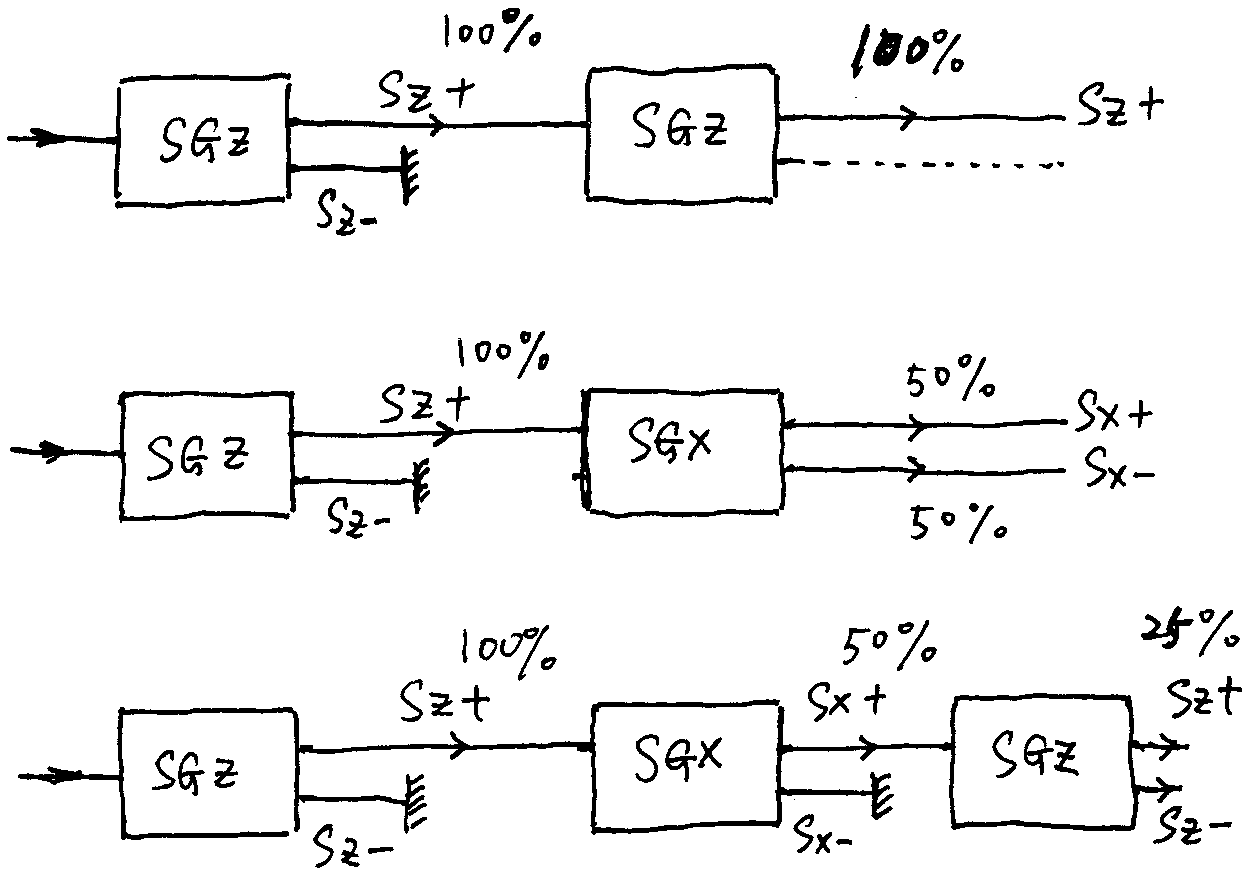
\includegraphics[width=10cm]{Spin/sequentialSGs.png}
\caption{连续的斯特恩-盖拉赫实验。}
%\label{default}
\end{center}
\end{figure}

现在我们使这些实验组合起来,比如:

先让银原子通过SGz,银原子分成对称的两束,我们用隔板挡住$s_z = -\frac{1}{2} \hbar$的那束,只让$s_z = \frac{1}{2} \hbar$的那一束出射,这个动作就是一个选择或过滤的动作。好比我们在一个篮子里放了一堆水果,有香蕉也有苹果,我们现在做一个选择,丢掉香蕉,把苹果留下来。

我们把这种专门选择$s_z = \frac{1}{2}\hbar$的斯特恩-盖拉赫装置记为SGz+,类似地还有SGz-,专门选择$s_z = - \frac{1}{2}\hbar$的银原子。类似地我们还可以定义SGx+,SGx-,SGy+和SGy-。

现在我们来做这样的组合实验:

\begin{equation*}
Ag \to SGz+ \to SGz+ \to ?
\end{equation*}

我们现在使用狄拉克的记号,把$s_z = \frac{1}{2}\hbar$的银原子用记号$\left| z+ \right\rangle$表示。我们用$\left| { ... } \right\rangle$表示量子力学的一个态,括号里面放上可以描述这个态的参数,现在就是z+,和银原子束如何在$z$方向上发生偏转有关。

让银原子束先通过SGz+,即把$\left| z+ \right\rangle$的态选择出来,然后再通过一次SGz+,还是选择$\left| z+ \right\rangle$,最后出射的还是$\left| z+ \right\rangle$。

现在考虑组合:

\begin{equation*}
Ag \to SGz+ \to SGz- \to ?
\end{equation*}

这个组合的作用是先选择$\left| z+ \right\rangle$,再试图从$\left| z+ \right\rangle$中选择$\left| z- \right\rangle$,实验表明最终没有任何银原子出来。这说明:$\left| z+ \right\rangle$和$\left| z- \right\rangle$是两个不相容的态,$\left| z+ \right\rangle$里面完全没有$\left| z- \right\rangle$,$\left| z- \right\rangle$里面完全没有$\left| z+ \right\rangle$。

这就好像是两个互相垂直的矢量$A, B$,A向B投影,或B向A投影都是0,我们可以说A里面完全没有B的成分,相反B里面也完全没有A的成分。

同时把任意的态$\left| \alpha \right\rangle$分解为$\left| z+ \right\rangle$和$\left| z- \right\rangle$的线性组合又是完备的,因为我们使银原子通过SGz时只得到了对称的两束,换句话说在这个标准下对银原子分类只能得到两类。

~

%需要提醒的是,以上陈述都是对实验的陈述,虽然我们有时会用推测式的语气。

下面我们在SGz+和SGz-之间插入一个SGx+:

\begin{equation*}
Ag \to SGz+ \to SGx+ \to SGz- \to ?
\end{equation*}

$x$方向上的非均匀磁场意味着变换了筛选法则。当然我们还可以推测,比如我们把$SGz \pm$想象为对水果种类的筛选,而$SGx \pm$想象为对水果颜色的筛选,那么我们有可能从“红苹果”中找出“香蕉”吗?在这种推测下,我们会认为没有银原子束出射。但最终结果只能实验说了算,实验表明有$\left| z- \right\rangle$态的银原子出来。

类似地,我们还可以做这样的实验:

\begin{center}

$Ag \to SGz+ \to SGx - \to SGz- \to ?$

$Ag \to SGz+ \to SGy + \to SGz- \to ?$

$Ag \to SGz+ \to SGy - \to SGz- \to ?$

$Ag \to SGx+ \to SGy - \to SGx- \to ?$

……

\end{center}

它们都会有银原子出来。

我们管这样的实验叫“连续的斯特恩-盖拉赫实验”(sequential Stern-Gerlach experiment)。

~

现在的问题是如何解释实验。

如果我们认为$\left| z+, x+ \right\rangle$这样的态存在的话,即存在一个对自旋态(我们从现在开始不说银原子了)的陈述,我们可以同时说$s_z = \frac{1}{2}\hbar$而且$s_x = \frac{1}{2}\hbar$,那么我们就没法从$\left| z+, x+ \right\rangle$中筛选出$\left| z- \right\rangle$。

%%

为了理解连续的“斯特恩-盖拉赫实验”,我们只有求助于比喻,即用我们熟悉的现象来类比,而建立比喻并不需要两种现象很像或……,所谓比喻是可以任意建立的,比如这里我们可以建立一个“颜色-形状”比喻来理解连续的“斯特恩-盖拉赫实验”。

假想在黑箱里有一堆小物件,我们应如何对其分类呢?比如颜色是一个分类的标准,形状是另一个分类的标准,颜色和形状是完全不相干的描述物件性质的两个标准。

我们说一个小物件是白色的;或是黑色的;白色和黑色是两种互相排斥的陈述,只要是白色的就不能是黑色的,相反只要是黑色的就不能是白色的。

我们也说一个小物件是个立方体,或说它是个球体。球体和立方体也是互相排斥的,我们没法说它既是球体又是立方体。

假设在我们的世界里,这个小物件不是立方体就是球体,但不能既是立方体又是球体。类似的我们说在我们的世界里,这个小物体不是白色的就是黑色的,但不能既是白色的又是黑色的。

形状是我们对物件的陈述,颜色也是我们对物件的陈述。现在我们的问题是:我们能够同时使用颜色和形状来陈述一个物件吗?

在经典世界里,或在我们的日常经验中,当然可以,香蕉是黄色的,同时它也是弯曲的棒棒形,形状和颜色是我们一眼看去可以直观的。

但在量子世界里,这种陈述是被禁止的!看清楚了物件的颜色,物件就完全没有形状;同样看清楚了物件的形状,那它就没有颜色\footnote{使用苹果、香蕉的语言:

设想我们先筛选出苹果,然后换个筛选标准,对苹果按颜色筛选,筛选出所有“红色的苹果”,注意!问题就在这里,一旦你说出了“红色的苹果”这一陈述,我们就没法从“红色的苹果”中筛选出香蕉了。

正确的陈述是:

我们首先筛选出苹果,然后换个筛选标准,对苹果按颜色筛选,但这两个标准是相克的,我们一旦知道了颜色,我们就完全丧失形状的信息,现在我们只知道是红色的,但完全不知道到底是苹果和香蕉,最后我们是对红色的水果筛选出香蕉。}。

这非常反直觉。但需记住,这种叙事是基于比喻建立的,如果我们换一个比喻的话,比如光的偏振现象,我们就会觉得一切都会来的很舒服。(对相同事件,切换视角,任意武断地使用比喻(图像)进行叙事是发现的门径。)

\subsubsection{与光偏振现象的类比}

我们现在来建立对连续斯特恩-盖拉赫实验的数学描述,考虑:

\begin{equation*}
Ag \to SGz+ \to SGx+ \to SGz- \to ?
\end{equation*}

假设银原子从SGz+出来的比例是100\%,通过SGx+后就只剩下50\%,然后通过SGz-还剩25\%银原子。

\begin{figure}[htbp]
\begin{center}
\includegraphics[width=10cm]{Spin/sequentiallightpolarization.png}
\caption{连续的偏振光实验}
%\label{default}
\end{center}
\end{figure}

我们可以通过与光偏振现象的类比来建立自旋的理论。光有线偏振光,还有圆偏振光。

比如我们使偏振片的偏振方向与x轴平行,它的作用就是使电矢量垂直于x轴的光统统被吸收,而电矢量平行于x轴的光全部通过。这样我们就得到一个x偏振的光,这也是筛选。

对一束x偏振的光而言,没有任何y偏振的成分,相反亦然,这可以类比态$\left|z+ \right\rangle $和$\left| z- \right\rangle$,它们都是互相排斥的分类标准。
 
~

现在使偏振片旋转$45^o$,我们称之为x'偏振片,它筛选出x'方向的偏振光,继续旋转$90^o$得到y'偏振片,筛选出y'偏振光,x'和y'是垂直的,因此x'偏振光中不会有任何y'的成分,反之亦然。

并且如果我们让一束光先通过x偏振片再通过x'偏振片,最后通过y偏振片的话,我们会看到出射光,而且百分比和刚才连续的斯特恩-盖拉赫实验的实验结果是一致的。

因此,我们就可以用x'偏振光来类比态$\left|x+ \right\rangle$,y'偏振光来类比$\left|x- \right\rangle$。

但我们还有态$\left| y+ \right\rangle$和$\left| y- \right\rangle$,它们应和什么样的偏振光来类比呢?

我们还有圆偏振光,R右旋光和L左旋光是互相排斥的分类标准,正好可以对应态$\left| y+ \right\rangle$和$\left| y- \right\rangle$。

现在我们的问题就转换为如何描述偏振光了,假设光沿$z$方向传播,光是横波,电矢量只能在$x-y$平面上振动,因此我们用$x-y$平面上的一个矢量来表示:

\begin{figure}[htbp]
\begin{center}
\includegraphics[width=8cm]{Spin/E0_projection.png}
\caption{振幅为$E_0$的x线偏振光先向x'方向投影,振幅变为$\frac{E_0}{\sqrt{2}}$,最后向y方向投影,振幅变为$\frac{E_0 }{2}$。光强正比于振幅的平方,因此光强的比为:100\% : 50\% : 25\%。}
%\label{default}
\end{center}
\end{figure}

$x-y$平面里的任意矢量可以表示为一个二维列向量,如矢量:

\begin{equation*}
V = 1 \cdot e_x + 0 \cdot e_y  \dot =\left( \begin{array}{ccc} 1 \\ 0 \end{array} \right) 
\end{equation*}

我们可以用一个二维的列向量来描述任意一束偏振光,但为了描述圆偏振光,列向量中必须出现纯虚数$i$,换句话说我们是用一个复系数的二维列向量来描述沿$z$方向传播的光的偏振态的。

%%

\begin{enumerate}
\item 

沿$z$轴传播的x线偏振光可表示为:

\begin{equation}
E^{x} = E_0 e_x \cos (k z - \omega t) 
\end{equation}

沿$z$轴传播的y线偏振光可表示为:

\begin{equation}
E^{y} = E_0 e_y \cos (k z - \omega t) 
\end{equation}

这里$e_x, e_y$分别是$x$轴和$y$轴上的单位向量。我们一般把它们写为列向量的形式,第一行对应$e_x$分量,第二行对应$e_y$分量。

\begin{eqnarray}
E^{x} & = & \left( \begin{array}{ccc} 1 \\ 0  \end{array} \right)  E_0 \cos (kz - \omega t )  \\
E^{y} & = & \left( \begin{array}{ccc} 0 \\ 1  \end{array} \right)  E_0 \cos (kz - \omega t )
\end{eqnarray}

再把它们改写为复数的形式。

\begin{eqnarray}
E^{x} & = & \Re \left( \begin{array}{ccc} 1 \\ 0  \end{array} \right)  E_0 e^{i ( kz - \omega t  )}  \\
E^{y} & = & \Re \left( \begin{array}{ccc} 0 \\ 1  \end{array} \right)  E_0 e^{i ( kz - \omega t  ) }  
\end{eqnarray}

\item

沿$z$轴传播的x'和y'线偏振光可表示为:

\begin{eqnarray}
E^{x'} & = & \Re \left( \begin{array}{ccc} 1 \\ 1  \end{array} \right)  \frac{ E_0 }{ \sqrt{2} }   e^{i ( kz - \omega t  )}  \\
E^{y'} & = & \Re \left( \begin{array}{ccc} -1 \\ 1  \end{array} \right)  \frac{E_0}{ \sqrt{2} }  e^{i ( kz - \omega t  ) }  
\end{eqnarray}

\item

沿$z$轴传播的右旋R圆偏振光和左旋L圆偏振光可表示为:

\begin{eqnarray}
E^{R} & = & \Re \left( \begin{array}{ccc} 1 \\ i  \end{array} \right)  \frac{ E_0 }{ \sqrt{2} }   e^{i ( kz - \omega t  )}  \\
E^{L} & = & \Re \left( \begin{array}{ccc} 1 \\  -i  \end{array} \right)  \frac{E_0}{ \sqrt{2} }  e^{i ( kz - \omega t  ) }  
\end{eqnarray}

\end{enumerate}

由于我们把自旋的态类比为光的偏振态,因此我们可以尝试把自旋的态表示为一个复系数二维向量空间中的一个向量。

\begin{enumerate}
\item 

我们分别用x线偏振光和y线偏振光来表示$\left| z+ \right\rangle$和$\left| z+ \right\rangle$。即尝试性地把$\left| z+ \right\rangle$表示为列向量$\left( \begin{array}{ccc} 1 \\ 0   \end{array} \right)$,把$\left| z- \right\rangle$表示为列向量$\left( \begin{array}{ccc} 0 \\ 1 \end{array} \right)$。即:

\begin{eqnarray}
\left| z+ \right\rangle & \dot = & \left( \begin{array}{ccc} 1 \\ 0   \end{array} \right) \\
\left| z- \right\rangle & \dot = & \left( \begin{array}{ccc} 0 \\ 1 \end{array} \right)
\end{eqnarray}

这里$\dot =$读作“表示为”,以示与“等于”的区分\footnote{等于只用于同类间的关系,而“表示为”或比喻则可用不同类的现象互为引证。}。

\item

态$\left| x \pm \right\rangle$可表示为:

\begin{eqnarray}
\left| x + \right\rangle & \dot = & \frac{1}{\sqrt{2}}  \left( \begin{array}{ccc}  1 \\ 1 \end{array}  \right)  \\
\left| x - \right\rangle  & \dot =  & \frac{1}{\sqrt{2}}  \left( \begin{array}{ccc}  -1 \\ 1 \end{array} \right)
\end{eqnarray}

\item

态$\left| y \pm \right\rangle$可表示为:

\begin{eqnarray}
\left| y + \right\rangle & \dot = & \frac{1}{\sqrt{2}}  \left( \begin{array}{ccc}  1 \\ i  \end{array} \right)  \\
\left| y - \right\rangle  & \dot =  & \frac{1}{\sqrt{2}}  \left( \begin{array}{ccc}  1 \\ -i \end{array} \right)
\end{eqnarray}

\end{enumerate}



\subsection*{练习}

\begin{enumerate}
\item 

斯特恩-盖拉赫实验,银原子束从温度为600K的炉子跑出来,经过准直装置后,通过一个0.1米长的非均匀磁场,磁场的梯度是$\frac{\partial B_z}{\partial z} = 10^3$特斯拉/米。银原子从非均匀磁场跑出来后又继续“飞”了1米,求最终银原子在靶上的分裂宽度是多少。(假设银原子的平均速度为$v$,它的平均动能是$\frac{M v^2}{2} = \frac{3 k_B T}{2}$,这里$M$是银原子的质量,$k_B$是玻尔兹曼因子。)

\end{enumerate}

\newpage

\section{投影和表示}

\subsection{太阳比喻}

在晴朗的日子里出去走一走,我们看不见自己,但却能看见自己的影子。这是很有意思的事情。

如果太阳不是很晒的话,我们可以站在一个空旷平坦的地上观察我们的影子,它和阳光射来的方向相对,在地上留下一个阴影,如果时间早的话,太阳升的不是很“高”,光线会斜斜地在地上投下一个较长的阴影,随着时间的流逝,太阳会沿着自己的轨道在天空中划出一个圆弧,随着太阳的升“高”,阴影会越来越短,当太阳升到最“高”的时候,阴影也最短。

但说高并不精确,我们可以把眼睛眯起,朝太阳的方向看,所谓“高”就是我们要仰起脖子才能“追踪”到太阳,我们仰起脖子的角度越大、太阳越高,我们可以把这个仰角定义为“太阳-观察者”连接线与地面的夹角$\theta$。当这个角度为$90^o$的时候,太阳在天顶,光线垂直地射下来,此时我们在地上的影子会“消失”\footnote{阴影之内没有光线是暗的,而阴影之外会被阳光照亮,光在这里更多地体现出“粒子性”,它以直线传播,绝对不会绕过障碍物。光从$\theta$方向照射到物体上,在地面上留下一个影子,假设物体的高度是$H$,影子的长度将是$H \cdot \frac{\cos \theta}{\sin \theta } = H \cdot \cot \theta$。}。

\begin{figure}[htbp]
\begin{center}
\includegraphics[width=5cm]{DiracNotation/sun_projection_1.png}
\caption{太阳光入射,与竖直方向成$\alpha$角。}
%\label{default}
\end{center}
\end{figure}


有时我们也以竖直的方向为基准,定义太阳光与竖直方向的夹角为$\alpha$($\alpha = \frac{\pi}{2} - \theta $),当$\alpha = 0$时,阳光笔直地照射在地面上,这时照射到单位面积上太阳光的能量最大,当角度$\alpha$逐渐增大时,照射到单位面积上太阳光的能量会变小,变小的比例正比于$\cos \alpha$。

人类走出非洲后,一路向北,先来到中近东,然后扩散到欧洲、亚洲等其它地方。中近东、欧洲、亚洲比非洲的纬度高,太阳会以一个更大的角度$\alpha$照射下来,随着$\alpha$的增大,单位表面积上地球吸收到的能量会减少,气温会随之降低,尤其是夜晚温度会更低。

我们现在都是住在屋子里的,但在远古人类甚至连制造房屋的技术都没有发明,冷了只能去山洞。但山洞里已经有其他动物占领了,比如曾广泛分布于欧洲和中近东各地的洞熊(cave bear)。洞熊的体型庞大,雄性洞熊的体重可高达1吨,可以想象与洞熊争夺山洞的战役是人类走出非洲后碰到的一大挑战。在这个过程中,火的使用是决定性的,因为在各种动物中只有人类不怕火,甚至还学会了使用火,发明了保存火种的方法,甚至制造火种的技术\footnote{维特鲁威在《建筑十书》中说:“远古时候,人类生来就像出没森林、洞穴和丛林中的野兽一样,茹毛饮血,辛苦度日。那时有一个地方,生长着密集繁茂的森林,狂风袭来,树木剧烈摇晃,树枝相互摩擦而起火。住在附近的人们被火焰吓坏了,逃之夭夭。但后来他们凑近时发现,火的热量对人体有极大的好处,他们将原木投入火中,将火种保存下来。”}。

可以想象人类曾长期生活在生有篝火的洞穴里,而这样的一个原始记忆也被用于比喻说理中,比如柏拉图在《理想国》中借用“洞穴”比喻了城邦和知识。

那么我们的洞穴经验是什么样的呢?

首先需要一个封闭的空间,比如在伸手不见五指的夜晚,任何一个房屋都可以是个洞穴,山洞无非也是个封闭的空间。

漆黑的夜晚,我们呆在山洞或封闭的房子里。我们什么都看不见,我们看不见自己,也看不见他人和物体。我们点燃一个火把或蜡烛。人是喜欢光亮的,于是都凑过去,此时我们在墙壁上看到影子,因为火把的光比较弱,反射一次后就基本没亮光了,洞穴中的影子会比阳光下的更显著和夸张,光和影在一起给我们的视觉极大的刺激。

阳光下我们不能清晰地看到物体的轮廓,但在洞穴经验中,阴影和光亮是截然分开的,我们甚至可以想象一个人去描摹阴影的轮廓。

用简单的线条去对象化一个物体是认识活动的开始,比如自我是不可见的,俗话说我们是在别人的眼睛(其实就是镜子)里认识自己的,但在洞穴经验里,我们在墙壁上能直接看见自己的阴影,比如我们可以面对着墙壁,背对着火把,伸出一只手,举过头顶……然后,我看见我面对的那个阴影会同步地作出这种种动作。

这就从视觉经验上把自我对象化了,同时我还能看见别人的阴影和其他物体的阴影……

火把的好处是可以随意移动,要想看清楚什么东西我们只需要把火把拿过来照一照就可以了。这意味着我们可以控制光线行进的方向,我可以让光向上方射,只需要我们把火把放在物体的下方,我们也可以让光向左射,只需要把火把放在物体的右边……

在洞穴中,我们举着火把从各个方向照物体,为的是要看清某物,光从某个方向射过来,我们看到的是光照亮的那个“面”,物体其他面的形象对我们是隐藏的,我们必须移动火把,使光从另外的方向射向物体,这个动作其实就是选择,我们选择从另一个角度“照亮”物体,刚才对我们显现的将隐藏在黑暗里,但新的面,新的形象会对我们显现。

\begin{figure}[htbp]
\begin{center}
\includegraphics[width=10cm]{DiracNotation/project_to_3D.png}
\caption{三视图就是往三个方向做投影。}
%\label{default}
\end{center}
\end{figure}

同时照亮所有的面则需要很多火把,比如我们可以从两个、三个,甚至六个方向上照亮物体。假设物体是三维的,并且假设物体是“透明”的,我们需要至少从三个互相垂直的方向上照亮物体,才能获得对物体的整体认识。这个其实就是工程里的三视图,上视、侧视和前视\footnote{假如物体不是透明的那就很复杂,因为还涉及物体内部构造的问题,即便不考虑内部构造,我们也得假设物体必须是“凸起”的,才能通过六视图获得物体的整体概念。}。

光源(太阳)、物体、阴影也构成一个常见的“认识论比喻”,这就是柏拉图的“太阳喻”。我们能“看”,是因为有光,而光是源自太阳的;光照射在物体上,我们像洞穴中背对着光源的原始人一样只能看到物体的阴影,即物体本身是不对我们显现的,对我们显现的只是物体的阴影。

这里我们的兴趣并不是介绍哲学上的“太阳喻”,我们只是借助这一图像建立量子力学中的“表示概念”。

在量子力学中没有物体,只有量子态,使用狄拉克记号,记作$\left| \alpha \right\rangle$,量子态本身是无法直接被“看”到的。我们需要对量子态建立一个表示,所谓表示就是选择一个观看的方式。

以观看物体为例,就是我们拿着火把以什么样的方式把物体仔细打量一番?比如我们可以选择从$x$,$y$,$z$三个方向上照亮物体,从三个方向照亮物体其实就是把物体对这三个方向做投影。

我们把矢量$V$看做是最简单的物体,往三个方向做投影就是:

\begin{quotation}
$x$方向,方向是$e_x$,投影是$V_x = e_x \cdot V$

$y$方向,方向是$e_y$,投影是$V_y = e_y \cdot V$

$z$方向,方向是$e_z$,投影是$V_z = e_z \cdot V$
\end{quotation}

我们把量子态想象成一个矢量(态矢量,state vector),它可能有很多“方向”,每个方向都有一个单位矢量,称作基矢,记为$\left| n \right\rangle$。

在量子力学中,态矢量$\left| \alpha \right\rangle $并不直接对应观测值,在这个意义下我们也说我们是“看不见”量子态的。但我们能“看见”态矢量的投影$\left\langle n | \alpha \right\rangle $,根据玻恩的统计解释,一个量子态处在$\left| n \right\rangle$态的几率正比于$\left|  \left\langle n | \alpha \right\rangle  \right|^2 $,我们管$\left\langle n | \alpha \right\rangle$叫几率幅\footnote{我们一般只讨论已经归一化了的量子态,所以就是等于了,即量子态$\left| \alpha \right\rangle$处在$\left| n \right\rangle$态的几率等于$\left\langle n | \alpha \right\rangle^2 $。}。

我们把投影算符$P_n$定义为:$\left| n \right\rangle \left\langle n \right|$,对量子态$\left| \alpha \right\rangle$投影的效果就是获得投影$\left| n \right\rangle \left\langle n | \alpha \right\rangle$。

\begin{figure}[htbp]
\begin{center}
\includegraphics[width=6cm]{DiracNotation/QM_sun_interpretation.png}
\caption{一个量子力学版的“太阳比喻”}
%\label{default}
\end{center}
\end{figure}

这里基矢$\{ \left| n \right\rangle \}$的选取是关键,它决定了观看方式,我们一般是通过构造一组和哈密顿$H$两两相互都对易的算符集$\{  H, A, B, ...  \}$来构造$\{ \left| n \right\rangle \}$的。

这样几率$\left| \left\langle n | \alpha \right\rangle \right|^2 $就有了明确的物理意义:

\begin{quotation}
现在我们把$\{ \left| n \right\rangle \}$改写成$\{ \left| E_n , a, b, ... \right\rangle  \}$,几率$\left|  \left\langle E_n, a, b | \alpha \right\rangle  \right|^2 $就是量子态$\left| \alpha \right\rangle $坍缩到态$\left| E_n, a, b \right\rangle$上的几率。
\end{quotation}

\begin{table}[htdp]
\caption{太阳比喻:哲学版本和量子力学版本}
\begin{center}
\begin{tabular}{|c|c|c|}
\hline
视觉 & 哲学 & 量子力学 \\
\hline
太阳 & 善(最高理念) & 研究纲领 \\
\hline
光线 & 逻各斯(Logos) & 投影算符$P_n $ \\
物体本身 & 理念 & 量子态 $\left| \alpha \right\rangle$ \\
阴影、影像 & 现象 & 几率幅 $\left\langle n | \alpha \right\rangle$ \\
眼睛,视觉能力 & 灵魂,求知能力 & 物理学家 \\ 
\hline
\end{tabular}
\end{center}
\label{default}
\end{table}%


\subsection{狄拉克记号}

下面我们将结合自旋1/2这个例子讨论量子力学中的狄拉克记号(Dirac Notation)。在理论物理学中记号法很重要,合适的记号法会使数学推导清晰简洁并且不容易出错。

狄拉克记号就是括号,括号在英文里是:

\begin{center}
bracket
\end{center}

我们把它表示为:

\begin{equation}
\left\langle  {bra}  \right|  {c} \left|   {ket}  \right\rangle 
\end{equation}

左边括号的“尖头”是向左的,我们称$\left\langle  {  }  \right|$是左矢空间(bra space)中的一个矢量(简称“左矢”),右边的括号的“尖头”是向右的,我们称$\left|  { }  \right\rangle $是右矢空间(ket space)中的一个矢量(简称“右矢”)。左矢和右矢中间夹着一个“内容”(content),这个内容是算符(operator),我们一般用大写字母$A$表示算符。

\begin{figure}[htbp]
\begin{center}
\includegraphics[width=4cm]{DiracNotation/bracket.png}
\caption{一个卡通化的“bra”和“cat”,即“胸罩”和“咪咪”。这个图对应的是“内积”。}
%\label{default}
\end{center}
\end{figure}

\subsubsection{向量、左矢和右矢}

针对自旋1/2的量子态,我们建立如下映射/表示关系:

\begin{eqnarray}
\left| + \right\rangle &\dot =& \left( \begin{array}{ccc} 1 \\ 0 \end{array} \right) \\
\left| - \right\rangle &\dot =& \left( \begin{array}{ccc} 0 \\ 1 \end{array} \right)
\end{eqnarray}

这里我们把$\left| z \pm \right\rangle$简记为$\left| \pm \right\rangle$,$\left| \pm \right\rangle$是互相排斥的同时完备的两个分类“标准”,任意的一个二维列向量$\left| \alpha \right\rangle$可以表示为它们的叠加:

\begin{equation}
\left| \alpha \right\rangle = a \left| + \right\rangle + b \left| - \right\rangle = \left( \begin{array}{ccc} a \\ b \end{array}  \right)
\end{equation}

这里的叠加系数$a$,$b$是复数(complex number)。在量子力学中我们用态矢量$\left| \alpha \right\rangle$表示系统的一个态。复数$c$是所谓对易数,它可以随便出现在列向量(态)的左边或者右边,或者我们把它和$\alpha$写在一起放在括号里面:

\begin{equation}
c \left| \alpha \right\rangle = \left| \alpha \right\rangle c = \left| c \alpha \right\rangle
\end{equation}

~

假设有两个向量$\left|  \alpha \right\rangle$、$\left| \beta \right\rangle$,我们想知道这两个向量的相似程度。如果在笛卡尔空间,我们让$\left|  \alpha \right\rangle$向$\left|  \beta \right\rangle$投影,记做:

\begin{equation}
\left|  \beta \right\rangle \left\langle \beta | \alpha  \right\rangle
\end{equation}

投影之后,向量在$\left| \beta \right\rangle$方向上,同时大小变成$\left\langle \beta | \alpha  \right\rangle$,即$\left| \alpha \right\rangle$在$\left| \beta \right\rangle$方向上的投影是$\left\langle \beta | \alpha  \right\rangle$倍的$\left| \beta \right\rangle$。

$\left\langle \beta | \alpha  \right\rangle$是个数,假如:

\begin{eqnarray*}
\left| \alpha \right\rangle &=& \left( \begin{array}{ccc} a \\ b \end{array} \right) \\
\left| \beta \right\rangle &=& \left( \begin{array}{ccc} c \\ d \end{array} \right)
\end{eqnarray*}

$\left\langle \beta | \alpha  \right\rangle$被定义为:

\begin{equation}
\left\langle \beta | \alpha  \right\rangle = \left( c^* , d^* \right) \left( \begin{array}{ccc}  a \\ b  \end{array}  \right) = c^* a + d^* b
\end{equation}

我们称$\left\langle \beta | \alpha  \right\rangle$为内积(inner product),这样定义内积的好处是会使向量$\left| \alpha \right\rangle$,自己和自己的内积——$ \left\langle \alpha | \alpha  \right\rangle $——是非负的。

\begin{equation*}
\left\langle \alpha | \alpha  \right\rangle = \left( a^* , b^* \right) \left( \begin{array}{ccc}  a \\ b  \end{array}  \right) = a^*a + b^* b \ge 0
\end{equation*}

如果向量$\left| \alpha \right\rangle$本身不是0向量,那么我们总可以把它归一化(normalized),归一化的因子是:

\begin{equation*}
\frac{1}{\sqrt { a^* a + b^* b }}
\end{equation*}

为了叙述的方便,下面我们引入几个术语(terminology):

\begin{enumerate}
\item 

$\left| \alpha \right\rangle$叫狄拉克“右矢”(ket),对每一个狄拉克右矢而言,都有一个狄拉克“左矢”(bra)与其对应,记作:$\left\langle \alpha \right|$。

\item

以二维复系数线性空间为例,一个狄拉克右矢可以表示为$\left| \alpha \right\rangle = \left( \begin{array}{ccc} a \\ b \end{array}  \right)$,与之对应的左矢$ \left\langle \alpha \right| $可表示为:$\left( a^* , b^*  \right)$。

即转置(transpose)再加复共轭(complex conjugate)。

转置的定义是:

\begin{equation}
\left( a_{ij}  \right)^T = \left( a_{ji} \right)
\end{equation}

即矩阵中“行变成列,列变成行”。比如:第一行第一列的元素,变到第一行第一列;第二行第一列的元素,变到第一行第二列。

复共轭的定义是:

\begin{equation}
\left( a_{ij}  \right)^* = \left( a_{ij}^* \right)
\end{equation}

即矩阵中每一个元素都取复共轭。

转置再加复共轭整体叫做厄米共轭(Hermite conjugate),表示为:

\begin{equation}
\left( a_{ij}  \right)^{\dagger} = \left( a_{ji}^* \right)
\end{equation}

\item

我们管$\left| \alpha \right\rangle  \leftrightarrow  \left\langle \alpha \right|$这样的关系叫“对偶”(dual correspondence),即对一个右矢而言存在一个左矢与之对应,相反对一个左矢而言也存在一个右矢与之对应。

\end{enumerate}

关于对偶,我们可以总结如下性质:

\begin{enumerate}
\item 

两向量相加的对偶:

\begin{equation}
\left| \alpha \right\rangle + \left| \beta \right\rangle  \leftrightarrow \left\langle \alpha \right| + \left\langle \beta \right|
\end{equation}

\item

复数乘一个向量的对偶:

\begin{equation}
c \left| \alpha \right\rangle  \leftrightarrow c^* \left\langle \alpha \right|
\end{equation}

\item

内积的对偶:

\begin{equation}
\left\langle \beta | \alpha \right\rangle = \left\langle \alpha | \beta \right\rangle^*
\end{equation}

\end{enumerate}

\subsubsection{算符}

算符(operator)就是操作,我们把算符定义为对矢量的操作,它把一个矢量映射为另一个矢量,比如它把一个右矢映射为另一个右矢:

\begin{equation}
A \left| \gamma \right\rangle = \left| \alpha \right\rangle \left\langle \beta |  \gamma \right\rangle =  \left\langle \beta |  \gamma \right\rangle  \left| \alpha \right\rangle = \left| \delta \right\rangle
\end{equation}

这里$ \left| \alpha \right\rangle \left\langle \beta \right| $,我们称之为两个向量的外积(outer product),就是算符$A$,它把右矢$\left|  \gamma \right\rangle$映射为$\left| \delta \right\rangle$。

\begin{equation}
A \left| \gamma \right\rangle = \left| \delta \right\rangle
\end{equation}

$\left| \delta \right\rangle$的对偶是$\left\langle  \delta \right|$,那么$A \left| \gamma \right\rangle$的对偶是什么呢?

我们把$A \left| \gamma \right\rangle$的对偶记作:

\begin{equation}
\left\langle \gamma \right| A^\dagger = \left\langle \delta \right|
\end{equation}

为了避免运算中出错,这里算符$A^\dagger$看作是向右——即对右矢——起作用的。

我们称$A^\dagger $是$A$的厄米共轭,并且$A$与$A^\dagger $互为厄米共轭。

下面我们来做几个练习:

\begin{enumerate}
\item 

$A = \left| \alpha \right\rangle \left\langle \beta \right|$,那么$A^\dagger = ?$

解:

把$A$作用于任意右矢$\left| \gamma \right\rangle$,然后求它的对偶:

\begin{equation*}
\left| \alpha \right\rangle \left\langle \beta | \gamma \right\rangle \leftrightarrow \left\langle \beta | \gamma \right\rangle^* \left\langle \alpha \right| = \left\langle \gamma | \beta \right\rangle \left\langle \alpha \right|
\end{equation*}

同时我们又有厄米共轭的定义:

\begin{equation*}
A \left| \gamma \right\rangle \leftrightarrow \left\langle \gamma \right|   A^\dagger
\end{equation*}

因此:

\begin{equation}
\left(  \left| \alpha \right\rangle \left\langle \beta \right|  \right)^\dagger = \left| \beta \right\rangle \left\langle \alpha \right|
\end{equation}


\item

定义两算符的相乘$AB $为

\begin{equation}
AB \left| \alpha \right\rangle = A \left( B \left| \alpha \right\rangle  \right)
\end{equation}

那么$AB$整体的厄米共轭$(AB)^\dagger = ?$

解:

先考虑$B$对$\left| \alpha \right\rangle$的作用$\left| \beta \right\rangle =  B \left| \alpha \right\rangle$,它的对偶是:

\begin{equation*}
\left| \beta \right\rangle = B \left| \alpha \right\rangle \leftrightarrow \left\langle \beta \right| = \left\langle \alpha \right| B^\dagger
\end{equation*}

现在考虑$AB \left| \alpha \right\rangle$的对偶:

\begin{equation*}
A B \left| \alpha \right\rangle = A \left| \beta \right\rangle \leftrightarrow \left\langle \beta \right| A^\dagger = \left\langle \alpha \right| B^\dagger A^\dagger 
\end{equation*}

同时我们又知道:

\begin{equation*}
A B \left| \alpha \right\rangle  \leftrightarrow \left\langle \alpha \right|  \left( AB \right)^\dagger 
\end{equation*}

因此:

\begin{equation}
\left(  AB \right)^\dagger = B^\dagger A^\dagger 
\end{equation}

\item

定义厄米算符为:

\begin{equation}
A^\dagger = A
\end{equation}

即:如果一个算符$A$的厄米共轭$A^\dagger $就是它自己的话,我们就说它是厄米的(Hermitian)。

证明如下等式对厄米算符成立:

\begin{equation}
\left\langle \beta \right| A \left| \alpha \right\rangle =  \left\langle \alpha \right| A \left| \beta \right\rangle^*
\end{equation}

证:

\begin{equation*}
\left\langle \beta \right| A \left| \alpha \right\rangle = \left\langle \beta \right|  \left( A \left| \alpha \right\rangle \right)  =   \{ \left(  \left\langle \alpha \right| A^\dagger \right) \left| \beta \right\rangle \}^* 
\end{equation*}

考虑到$A$是厄米的,$A^\dagger = A$:

\begin{equation*}
\left\langle \beta \right| A \left| \alpha \right\rangle = \left\langle \alpha \right| A \left| \beta \right\rangle^*
\end{equation*}

假如$\left| \beta \right\rangle = \left| \alpha \right\rangle$的话,

\begin{equation*}
\left\langle \alpha \right| A \left| \alpha \right\rangle = \left\langle \alpha \right| A \left| \alpha \right\rangle^*
\end{equation*}

一个数的复共轭就是这个数自己,这说明$\left\langle \alpha \right| A \left| \alpha \right\rangle$是个实数(real number)。

由于物理可观测量的数值必须是实数(而不能是复数),在量子态$\left| \alpha \right\rangle$下,$\left\langle \alpha \right| A \left| \alpha \right\rangle$就可以用来表示物理量A的期望值(expectation value),前提是我们必须用一个厄米算符$A$来表示物理量A。

\end{enumerate}



\subsubsection{本征值问题}

考虑:

\begin{equation}
A \left| a' \right\rangle = a' \left| a' \right\rangle
\end{equation}

即:算符作用于右矢上,其后果是这个算符自身再乘上一个复数,于是这个复数就可用来标记(命名)这个右矢。

$a'$叫做本征值(eigen value),$\left| a' \right\rangle$叫做本征矢(eigen vector),$\left| a' \right\rangle$是与$a'$对应的本征矢。把所有符合$A \left| a' \right\rangle = a' \left| a' \right\rangle$条件的$a'$及其对应的$\left| a' \right\rangle $都求出来的挑战叫做“求解本征值问题”。

我们可以证明,假如$A$是厄米算符的话,其本征值$a'$一定是实数。并且如果有两个本征值$a'$和$a''$,假如$a' \neq a''$的话,它们对应的本征矢$\left\langle a' | a'' \right\rangle = 0$,即$\left| a' \right\rangle$和$\left| a'' \right\rangle$一点都不像。

证:

由本征值问题:

\begin{equation*}
A \left| a' \right\rangle = a' \left| a' \right\rangle
\end{equation*}

出发。其对偶形式是:

\begin{equation*}
\left\langle a'' \right| A^\dagger =  \left\langle a'' \right| A = a''^* \left\langle a'' \right|
\end{equation*}

再把上式作用于右矢$\left| a' \right\rangle$

\begin{equation*}
\left\langle a'' \right| A \left| a' \right\rangle = a' \left\langle a'' | a' \right\rangle = a''^* \left\langle a'' | a' \right\rangle
\end{equation*}

整理一下:

\begin{equation*}
\left( a' - a''^* \right) \left\langle a'' | a' \right\rangle = 0
\end{equation*}

假如$a'$就是$a''$的话,只要$\left| a' \right\rangle$不是0矢量,$\left\langle a' | a' \right\rangle > 0 $,因此:

\begin{equation*}
a' = a'^*
\end{equation*}

一个数的复共轭就等于这个数自己,这意味着这个数的虚部为0,或这个数是实数。

现在假设$a' \neq a''$,同时利用刚刚证明出的结果$a'$和$a''$都是实数,考虑:

\begin{equation*}
\left( a' - a'' \right) \left\langle a''  | a'  \right\rangle = 0
\end{equation*}

因为$a' - a'' \neq 0$,内积$\left\langle a''  | a'  \right\rangle$就必须为0。

~

假设$\left| a' \right\rangle$是$A$的本征矢,任意乘一个复数,$c \left| a' \right\rangle$也是$A$的本征矢,一般我们提到的本征矢$\left| a' \right\rangle$都是归一化的本征矢。

根据以上证明,算符$A$的所有本征矢$\left| a' \right\rangle$构成一个集合$\{ \left| a' \right\rangle \}$,并且满足正交归一(orthonormal)的关系。

\begin{equation}
\left\langle a' | a'' \right\rangle = \delta_{a', a''}
\end{equation}

这里$\delta_{a', a''}$是克罗尼克记号,当$a' = a''$时,$\left| a' \right\rangle$是归一的,即$\delta_{a', a''} = 1$;当$a' \neq a''$时,$\left| a' \right\rangle$和$\left| a'' \right\rangle$是正交的,即$\delta_{a', a''} = 0$。

~

这里我们忽略了一种情况,即一个本征值$a'$,它有可能对应多个不同的本征矢量,比如$\left| a'_1 \right\rangle $、$\left| a'_2 \right\rangle $……$\left| a'_f \right\rangle$。一个本征值和$f$个不同的本征矢量对应,我们称这种情况为简并,简并度为$f$。

对于存在简并的本征值问题,原则上我们也能得到一个正交归一的本征矢的集合$\{ \left| a' \right\rangle \}$,难的是给它们起名字,或做标记。

因为一个$a'$有可能对应好几个不同的$\left| a'_1 \right\rangle $、$\left| a'_2 \right\rangle $、……,仅仅靠$a'$我们是无法分辨它们的。

这就要求我们考虑新的本征值问题。比如,考虑算符$B$的本征值问题,为了使$B$及其对应的分类命名体系在物理上有意义,我们要求$B$也是个厄米算符。

假设$A$和$B$是对易的,即

\begin{equation}
AB = BA
\end{equation}

$A$的本征值问题存在简并,即存在某个本征值$a'$,有$\left| a'_1 \right\rangle$,$\left| a'_2 \right\rangle$,……,$\left| a'_f \right\rangle$,$f$个不同的本征矢与$a'$对应,现在的关键是找到给它们标记的方案,光靠$A$的本征值$a'$是不够的。

首先,对$i = 1, 2,... f$,我们有:

\begin{equation}
A \left| a'_i \right\rangle = a' \left| a'_i \right\rangle 
\end{equation}

我们定义这$f$个不同的本征矢的线性叠加$\left| \alpha \right\rangle $:

\begin{equation}
\left| \alpha \right\rangle = \sum\limits_i c_i \left| a'_i \right\rangle
\end{equation}

对$\left| \alpha \right\rangle $,我们依然有:

\begin{equation}
A \left| \alpha \right\rangle  = a' \left| \alpha \right\rangle
\end{equation}

考虑到$A$,$B$对易:

\begin{equation}
AB \left| \alpha \right\rangle = B A \left| \alpha \right\rangle = a' B \left| \alpha \right\rangle
\end{equation}

上式中最左边的一项和最右边的一项说明$B \left| \alpha \right\rangle $依然是$A$的本征矢。

假设算符$B$满足关系:$B \left| \alpha \right\rangle = b' \left| \alpha \right\rangle$,求解本征值问题:

\begin{equation}
B \left| \alpha \right\rangle = b' \left| \alpha \right\rangle
\end{equation}

$\left| \alpha \right\rangle$可以表示为一个$f$维的列向量。

\begin{equation}
\left| \alpha \right\rangle \dot = \left( \begin{array}{ccc} c_1 \\ c_2 \\ ... \\ c_f  \end{array} \right)
\end{equation}

我们需要求解的线性代数问题是:

\begin{equation}
\left( B - b' I \right) \left( \begin{array}{ccc} c_1 \\ c_2 \\ ... \\ c_f  \end{array} \right)  = 0
\end{equation}

如果我们要求关于$\left( \begin{array}{ccc} c_1 \\ c_2 \\ ... \\ c_f  \end{array} \right)$的非零解,我们就得要求如下行列式为0:

\begin{equation}
\det \left( B - b' I \right) = 0
\end{equation}

这是一个关于$b'$的一元$f$次方程。

幸运的话,我们能求出$f$个不同的$b'$的取值,$b'_1, b'_2, ... b'_f$。把$b'$值代回方程我们能得到不同的本征矢,记作$\left| a', b'_i \right\rangle$,$i = 1, 2, ...f$。

~

我们一般会笼统地把$A$,$B$的共同本征态记作$\left| a', b' \right\rangle$,

%但也可能求不出$f$个不同的$b'$,我们可以笼统地把$A$,$B$的共同本征态记作$\left| a', b' \right\rangle$,

%存在$A$,$B$的共同本征态$\left| a', b' \right\rangle$使得:

\begin{eqnarray}
A \left| a', b' \right\rangle &=& a' \left| a', b' \right\rangle \\
B \left| a', b' \right\rangle &=& b' \left| a', b' \right\rangle
\end{eqnarray}

在引入新的指标$b'$后,$a', b'$在一起就有可能把简并消除掉,即不同的本征矢$\{  \left| a', b' \right\rangle  \}$可以和指标$\{ a', b' \}$构成“一一对应”。

如果还存在简并的话,原则上我们可以引入更多两两都对易的厄米算符的集合;由于在量子力学中我们用厄米算符表示物理量,我们也说找到一个“两两都对易的力学量(或物理量)的集合”,$\left( H, A, B, ...  \right)$。

这里总会包括哈密顿算符$H$,因为哈密顿算符对应能量,在物理里我们最关心能量,比如对求解氢原子的量子力学问题,我们会取这样一个两两都对易的力学量的集合$\left( H, L^2, L_z  \right)$。

$H$对应的是主量子数$n$,对应的本征值问题是:

\begin{equation}
H \left| n \right\rangle = E_n \left| n \right\rangle 
\end{equation}

$L^2$是轨道角动量算符的平方,$L_z$是轨道角动量算符在$z$方向上的分量,对应的本征值问题是:

\begin{eqnarray}
L^2 \left| l, m \right\rangle & = & l (l + 1 )\hbar^2 \left| l, m \right\rangle \\
L_z \left| l, m \right\rangle & = & m \hbar \left| l, m \right\rangle
\end{eqnarray}

$n, l, m$一起构成了对氢原子量子态$\left| n, l, m \right\rangle$进行描述的恰当语言。(所谓恰当就是分类的合理,每个不同的对象都有命名,而命名和命名之间有绝不重复)

所有的$\left| n, l, m \right\rangle$,两两都是正交归一的:

\begin{equation}
\left\langle n', l', m' | n, l, m \right\rangle = \delta_{nn'} \delta_{ll'} \delta_{mm'}
\end{equation}

它们的集合$\{ \left| n, l, m \right\rangle \}$构成了基矢(basisi),任意用$H$描述的物理系统的量子态可以表示为$\{ \left| n, l, m \right\rangle \}$的线性叠加。

\subsubsection{投影算符}

假设$\{  \left| n \right\rangle \}$构成基矢,基矢就相当于笛卡尔坐标系里的$\{ i, j, k \}$

笛卡尔坐标系里的任意向量$V$可以表示为向$i$($x$方向的单位矢量),$j$($y$方向的单位矢量),$k$($z$方向的单位矢量)三个方向的投影之和。

\begin{equation}
V = i V_x + j V_y + k V_z
\end{equation}

这里$V_x$是$V$向$i$的投影,表示为$V \cdot i$,我们也可以把它们按照狄拉克记号的形式进行改写:

\begin{equation}
\left| V \right\rangle =\left| i \right\rangle \left\langle i | V \right\rangle + \left| j \right\rangle \left\langle j | V \right\rangle + \left| k \right\rangle \left\langle k | V \right\rangle
\end{equation}

这里的$\left| i \right\rangle \left\langle i \right|$,$\left| j \right\rangle \left\langle j \right|$和$\left| k \right\rangle \left\langle k \right|$就是投影算符,分别表示把向量$\left| V \right\rangle $向$\left| i \right\rangle $,$\left| j \right\rangle $或$\left| k \right\rangle $投影的动作。

向所有方向投影再加起来就是单位算符$I$

\begin{equation}
I = \left| i \right\rangle \left\langle i \right| + \left| j \right\rangle \left\langle j \right| + \left| k \right\rangle \left\langle k \right|
\end{equation}

对量子力学而言,我们的基矢是$\left| n \right\rangle $,投影算符$P_n$是:

\begin{equation}
P_n = \left| n \right\rangle \left\langle n \right|
\end{equation}

表示向第$n$个基矢$\left| n \right\rangle$的投影动作。

单位算符是:

\begin{equation}
I = \sum\limits_n \left| n \right\rangle \left\langle n \right|
\end{equation}

这个表达式是量子力学中最重要的公式,因为我们可以选择不同的分类体系(其实就是表象),这样我们就可以让物理陈述在不同的表象间变换。

\subsubsection{幺正算符}

考虑一个已经被归一化了的量子态$\alpha$,

\begin{equation}
\left\langle \alpha | \alpha \right\rangle = 1
\end{equation}

假设态可以经历一个变化,这个变化用算符$U$表示,它使得:

\begin{eqnarray*}
\left| \alpha \right\rangle & \to & U \left| \alpha \right\rangle \\
\left\langle \alpha \right| & \to & \left\langle \alpha \right| U^\dagger
\end{eqnarray*}

假设我们考虑的物理过程$U$不会导致粒子的产生和湮灭,即:

\begin{equation}
\left\langle \alpha | \alpha \right\rangle \to  \left\langle \alpha \right| U^\dagger U \left| \alpha \right\rangle = 1
\end{equation}

这意味着$U$满足:

\begin{equation}
U^\dagger U = I
\end{equation}

这里$I$表示单位算符,但我们往往也把单位算符就简单地写作1,实际上在进行推导的时候,必要的简略是不可避免的,甚至如何简略公式的表达本来就是物理思维的一部分。

满足关系$U^\dagger U = 1$的算符$U$是幺正算符(Unitary operator),一般来说幺正算符不是厄米算符。

%并不仅仅是厄米算符才在量子力学中有用。

\subsection{自旋的泡利矩阵表示}

回到自旋1/2的例子,我们定义自旋算符$S$为

\begin{equation}
S = i S_x + j S_y + k S_z
\end{equation}

这里的$S_z$是自旋算符在$z$方向上的分量,它可定义为:

\begin{equation}
S_z = \frac{\hbar}{2} \left( \left| + \right\rangle \left\langle + \right| - \left| - \right\rangle \left\langle - \right|  \right)
\end{equation}

它使得:

\begin{eqnarray}
S_z \left| + \right\rangle &=& \frac{\hbar}{2} \left| + \right\rangle \\
S_z \left| - \right\rangle &=& - \frac{\hbar}{2} \left| - \right\rangle
\end{eqnarray}

这对应$z$方向的非均匀磁场(SGz)可以把“非极化”的Ag原子束分裂为相等percentage的上下两束。

我们还可以写出$S_z$的矩阵表示:

\begin{equation}
S_z =  \frac{\hbar}{2} \left( \begin{array}{ccc}  1 & 0 \\ 0 & 1   \end{array}  \right)
\end{equation}

~

我们把$S_x$定义为:

\begin{equation}
S_x = \frac{\hbar}{2} \left( \left| x+ \right\rangle \left\langle x+ \right| - \left| x- \right\rangle \left\langle x- \right| \right)
\end{equation}

这意味着$x$方向的非均匀磁场(SGx)可以把“非极化”的Ag原子束分裂为相等percentage的“左右”两束。

我们一般取$\left| z+ \right\rangle = \left| + \right\rangle = \left( \begin{array}{ccc} 1 \\ 0 \end{array} \right)  $,$\left| z- \right\rangle = \left| + \right\rangle = \left( \begin{array}{ccc} 0 \\ 1 \end{array} \right)  $,这种对基矢的取法叫$S_z$表象。这意味着$S_x$的矩阵表示就不能是对角的了。

我们可以这么来计算$S_x$的矩阵表示:

\begin{equation}
S_x \dot = \left( \begin{array}{ccc}  \left\langle + \right| S_x \left| + \right\rangle  &  \left\langle + \right| S_x \left| - \right\rangle \\   \left\langle - \right| S_x \left| + \right\rangle  &   \left\langle - \right| S_x \left| - \right\rangle  \end{array} \right) 
\end{equation}

利用:

\begin{eqnarray*}
\left| x+ \right\rangle  & = & \frac{1}{\sqrt{2}} \left(  \begin{array}{ccc} 1 \\ 1  \end{array} \right) \\
\left| x- \right\rangle & = &  \frac{1}{\sqrt{2}} \left(  \begin{array}{ccc} -1 \\ 1  \end{array} \right)
\end{eqnarray*}

我们可以计算比如矩阵中的第一项:

\begin{eqnarray*}
\left\langle + \right| S_x \left| + \right\rangle &=& \frac{\hbar}{2} \left( \left\langle + | x+ \right\rangle \left\langle x+ | + \right\rangle - \left\langle + | x- \right\rangle \left\langle x- | + \right\rangle   \right) \\
{} &=& \frac{\hbar}{2} \left( \frac{1}{2} - \frac{1}{2} \right) = 0
\end{eqnarray*}

最终计算出$S_x$的矩阵表示是:

\begin{equation}
S_x  = \frac{\hbar}{2} \left( \begin{array}{ccc} 0 &  1 \\ 1 & 0 \end{array} \right)
\end{equation}

~

我们把$S_y$定义为:

\begin{equation}
S_y = \frac{\hbar}{2} \left( \left| y+ \right\rangle \left\langle y+ \right| - \left| y- \right\rangle \left\langle y- \right| \right)
\end{equation}

其矩阵表示为:

\begin{equation}
S_y \dot = \left( \begin{array}{ccc}  \left\langle + \right| S_y \left| + \right\rangle  &  \left\langle + \right| S_y \left| - \right\rangle \\   \left\langle - \right| S_y \left| + \right\rangle  &   \left\langle - \right| S_y \left| - \right\rangle  \end{array} \right) = \frac{\hbar}{2} \left( \begin{array}{ccc} 0 &  -i \\ i & 0 \end{array} \right) 
\end{equation}

小结一下:

\begin{eqnarray}
S_x &=& \frac{\hbar}{2} \sigma_x =  \frac{\hbar}{2} \left( \begin{array}{ccc} 0 &  1 \\ 1 & 0 \end{array} \right)  \\
S_y &=& \frac{\hbar}{2} \sigma_y = \frac{\hbar}{2} \left( \begin{array}{ccc} 0 &  -i \\ i & 0 \end{array} \right)  \\
S_z &=& \frac{\hbar}{2} \sigma_z = \frac{\hbar}{2} \left( \begin{array}{ccc} 1 &  0 \\ 0 & -1 \end{array} \right)  
\end{eqnarray}

这里$\sigma_x = \left( \begin{array}{ccc} 0 &  1 \\ 1 & 0 \end{array} \right) $,$\sigma_y = \left( \begin{array}{ccc} 0 &  -i \\ i & 0 \end{array} \right) $,$\sigma_z = \left( \begin{array}{ccc} 1 &  0 \\ 0 & -1 \end{array} \right) $。再加上单位矩阵$I =  \left( \begin{array}{ccc} 1 &  0 \\ 0 & 1 \end{array} \right)$,总共四个合称泡利矩阵(Pauli matrices)。

%任意一个$2 \times 2$的厄米矩阵都可以表示为以上四个泡利矩阵的线性叠加。

%这是因为一个$2 \times 2$的厄米矩阵可表示为:

%\begin{equation}
%\left( \begin{array}{ccc}  a  & c+ id  \\  c- i d & b  \end{array} %\right)
%\end{equation}

%这里$a, b, c, d$都是实数,正好对应四个独立的变量。

~

我们可以验证自旋$S$确实符合角动量的性质:

\begin{eqnarray}
\left[ S_x , S_y  \right]  & = & i \hbar S_z\\
\left[ S_y , S_z  \right]  & = & i \hbar S_x\\
\left[ S_z , S_x  \right]  & = & i \hbar S_y\\
\left[S_x , S^2 \right] & = & \left[S_y , S^2 \right] = \left[S_z , S^2 \right] =  0
\end{eqnarray}

~

升降算符$S^+$和$S^-$可以大大简化涉及自旋算符的量子力学计算:

%我们定义升降算符$S^+$和$S^-$为:

\begin{eqnarray}
S^+ & = & \hbar  \left| + \right\rangle \left\langle - \right|  \\
S^- & = & \hbar  \left| - \right\rangle \left\langle + \right|
\end{eqnarray}

$S^+$的作用是使$\left| - \right\rangle$ 变成 $\left| + \right\rangle$,

\begin{equation}
S^+ \left| - \right\rangle = \hbar  \left| + \right\rangle \left\langle -  | -   \right\rangle = \hbar \left| + \right\rangle
\end{equation}

$S^-$的作用是使$\left| + \right\rangle$ 变成 $\left| - \right\rangle$,

\begin{equation}
S^- \left| + \right\rangle = \hbar  \left| - \right\rangle \left\langle +  | +   \right\rangle = \hbar \left| - \right\rangle
\end{equation}

升降算符是极形象的命名。

我们可以把“升降算符”表示为一个$2 \times 2$的方阵,它使得一个“$2 \times 2$的方阵”乘以一个“二维列向量”等于一个“二维列向量”,这就是算符的“矩阵表示”。

比如$S^+$的矩阵表示是:

\begin{equation}
S^+ \dot = \left(  \begin{array}{ccc}  S^+_{++} &  S^+_{+-} \\  S^+_{-+} & S^+_{--}  \end{array} \right)
\end{equation}

这里的矩阵元分别是:

\begin{eqnarray*}
S^+_{++} &=& \left\langle + \right| S^+ \left| + \right\rangle = \hbar \left\langle + | +  \right\rangle  \left\langle  - | + \right\rangle = 0 \\
S^+_{+-} &=&  \left\langle + \right| S^+ \left| - \right\rangle = \hbar \left\langle + | + \right\rangle  \left\langle - | - \right\rangle = 1 \\
S^+_{-+} &=& \left\langle - \right| S^+ \left| + \right\rangle = \hbar \left\langle - | + \right\rangle \left\langle - | + \right\rangle = 0 \\
S^+_{--} &=&  \left\langle - \right| S^+ \left| - \right\rangle = \hbar \left\langle - | + \right\rangle \left\langle - | - \right\rangle = 0
\end{eqnarray*}

这里我们利用了:

\begin{eqnarray*}
\left\langle + | + \right\rangle & = & \left\langle - | - \right\rangle = 1 \\
\left\langle + | - \right\rangle & = & \left\langle - | + \right\rangle = 0
\end{eqnarray*}

因此,自旋1/2的升算符$S^+$可表示为:

\begin{equation}
S^+ \dot = \hbar \left(  \begin{array}{ccc}  0 &  1 \\  0 & 0  \end{array} \right)
\end{equation}

类似地,可求出降算符$S^-$的矩阵表示(或直接利用性质:$\left( S^+ \right)^\dagger = S^-$):

\begin{equation}
S^- \dot = \hbar \left(  \begin{array}{ccc}  0 &  0 \\  1 & 0  \end{array} \right)
\end{equation}

最后,我们可以验证:

\begin{equation}
S^{\pm} = S_x \pm i S_y
\end{equation}

\subsection{角动量的代数解法}

我们现在来求解$(L^2, L_z)$的共同本征值问题,通常来说这需要我们求解一个关于极角$\theta$和方位角$\phi$的偏微分方程,这是极啰嗦的,但我们也可由对易式出发,仅凭代数关系就把$(L^2, L_z)$的共同本征值问题求出来,而且我们发现在这个代数解法中,$l = 1/2$这样的解不再是不允许的了\footnote{由于代数解法中根本就不出现$\theta$和$\phi$,所以$l= 1/2$这样的解就是允许的。},这实际上给出了一个关于轨道角动量(量子数取整数)和自旋角动量(量子数取1/2)的共同描述。

假设$(L^2, L_z)$的共同本征态是$\left| \lambda, \mu  \right\rangle$,

\begin{eqnarray}
L^2 \left| \lambda, \mu \right\rangle &=& \lambda \hbar^2 \left| \lambda, \mu  \right\rangle \\
L_z \left| \lambda, \mu  \right\rangle &=& \mu \hbar \left| \lambda, \mu  \right\rangle
\end{eqnarray}


首先我们模仿自旋1/2的情形定义升降算符$L^{\pm}$:

\begin{eqnarray}
L^+ &=& L_x + i L_y  \\
L^- &=& L_x - i L_y 
\end{eqnarray}

我们可以证明对易式:

\begin{equation*}
[ L_z, L^+ ] = [L_z, L_x + i L_y] = L_z L^+ - L^+ L_z = \hbar L^+
\end{equation*}

利用:

\begin{equation*}
( L_z L^+ - L^+ L_z ) \left| \lambda, \mu  \right\rangle = \hbar L^+ \left| \lambda, \mu \right\rangle
\end{equation*}

考虑到:$L^+ L_z \left| \lambda, \mu \right\rangle = \mu \hbar L^+ \left| \lambda, \mu \right\rangle $,

\begin{equation}
L_z L^+ \left| \lambda, \mu \right\rangle = (\mu + 1) \hbar L^+ \left| \lambda, \mu \right\rangle
\end{equation}

这里我们把$L^+ \left| \lambda, \mu \right\rangle$看成是一个新的态矢量,它也是$L_z$的本征矢,本征值为$( \mu + 1 ) \hbar$,因此$L^+ \left| \lambda, \mu \right\rangle$可表示为:

\begin{equation}
L^+ \left| \lambda, \mu \right\rangle = C \left| \lambda, \mu+1 \right\rangle
\end{equation}

这里$C$是待定的复数因子。

即$L^+$可以使量子数$\mu+1$,我们形象地称之为升算符。类似地,我们可证明$L^- \left| \lambda, \mu \right\rangle $也是$L_z$的本征矢,对应本征值为$(\mu-1) \hbar$。

因此,$L^- \left| \lambda, \mu \right\rangle$可表示为:

\begin{equation}
L^- \left| \lambda, \mu \right\rangle = C' \left| \lambda, \mu-1 \right\rangle
\end{equation}

这里$C'$是待定的复数因子。

即$L^-$可以使量子数$\mu-1$,我们形象地称之为降算符。

现在的问题是这种“升、降”操作是否可无限制地进行下去?

如果可以的话,就意味着$L_z$的本征值的大小就没有限制了,而这是不可能的。因为$L_z$仅仅是$L = i L_x + j L_y + k L_z$算符的一个分量,而我们假设$L^2 = L_x^2 + L_y^2 + L_z^2$的本征值是$\lambda \hbar^2$,这样“升、降”操作就不能无限制地进行下去。

通俗地说就是我们假设角动量量子数是$l$,那么$\mu$的取值最大将只是$l$,再大是不可能的。

我们把这句话翻译成数学的语言,对态$\left| \lambda, l \right\rangle$,必须有:

\begin{equation}
L^+ \left| \lambda, l \right\rangle = 0
\end{equation}

对零矢量前面再乘一个算符$L^-$并不会改变计算结果,即:

\begin{equation}
L^- L^+ \left| \lambda, l \right\rangle = 0 
\end{equation}

我们把$L^- L^+$展开:

\begin{eqnarray*}
L^- L^+ &=& ( L_x - i L_y ) (L_x + i L_y) = L_x^2 + L_y^2 + i [ L_x, L_y ] \\
{} &=& L^2 - L_z^2 - \hbar L_z
\end{eqnarray*}

即:

\begin{equation}
L^2 \left| \lambda, l \right\rangle = (L_z^2 + \hbar L_z) \left| \lambda, l \right\rangle = l (l + 1)\hbar^2 \left| \lambda, l \right\rangle
\end{equation}

现在我们重新把$\lambda$写作$l (l +1)$,$\mu$重新写作$m$,$\left|  \lambda, \mu \right\rangle$写作$\left| l, m \right\rangle$,得到:

\begin{eqnarray}
L^2 \left| l,m \right\rangle &=& l(l+1)\hbar^2 \left| l,m \right\rangle \\
L_z \left| l,m \right\rangle &=& m \hbar \left| l,m \right\rangle
\end{eqnarray}

这里$m$的取值是从$l$开始逐渐“减1”,“减1”,最后得到对称的$-l$,或者我们由$-l$开始逐渐“加1”,“加1”,最后得到$l$。要得到这种结构,$l$取整数$0, 1, 2 ...$是可以的,取半整数$1/2, 3/2, ...$也是可以的,但取其他情况就不可以了。

小结一下:

\begin{eqnarray*}
l &=& 0, 1/2, 1, 3/2, 2, ...\\
m &=& l, l-1, ..., -l +1 , -l
\end{eqnarray*}

对轨道角动量而言$l$只能取整数,是我们这里讨论的一种特殊情况。

~

下面我们继续证明一个有用的性质,对升降算符$L^{\pm}$,有:

\begin{equation*}
L^{\pm} \left| l,m \right\rangle = \hbar \sqrt{(l \mp m)(l \pm m +1)
} \left|l, m \pm 1 \right\rangle
\end{equation*}

定义: $\left| \gamma \right\rangle = L^+ \left| lm
\right\rangle$, 对应到左矢空间, $\left\langle \gamma \right| =
\left\langle lm  \right| L^-$,

因此:

\begin{equation*}
\left\langle \gamma | \gamma \right\rangle = \left\langle lm \right|
L^- L^+ \left| lm \right\rangle
\end{equation*}

上式中的$L^- L^+$展开是:

\begin{equation*}
(L_x-iL_y) (L_x + i L_y) = L_x^2 + L_y^2 +i [L_x, L_y] = L^2 - L_z^2
- \hbar L_z
\end{equation*}

因此:

\begin{equation*}
\left\langle \gamma | \gamma \right\rangle = \left\langle L^2 -
L_z^2 - \hbar L_z \right\rangle = l(l+1)\hbar^2 - m^2\hbar^2 -m
\hbar^2
\end{equation*}

上式化简可得:

\begin{equation*}
\left\langle \gamma | \gamma \right\rangle =  (l - m)(l+m+1)\hbar^2
\end{equation*}

即:

\begin{equation}
L^+  \left| l, m \right\rangle = \hbar \sqrt{(l - m)(l + m +1) } \left|l, m + 1 \right\rangle
\end{equation}

类似地,我们还可对降算符$L^-$证明:

\begin{equation}
L^-  \left| l, m \right\rangle = \hbar \sqrt{(l + m)(l - m +1) } \left|l, m - 1 \right\rangle
\end{equation}

\subsection{自旋单态和自旋三重态}

假设有两个自旋,自旋甲和自旋乙,它们是独立的,所谓独立就是说甲的态不会影响乙,反过来乙的态也不会影响甲。但我们现在考虑的系统是“甲和乙”。对这样“甲和乙”的自旋的态我们应如何描述。

但考虑自旋甲的话,自旋甲可以是随便一个态$\left| \alpha \right\rangle$,如果我们使用$S_z$表象的话,我们取自旋甲在$z$方向向上和向下的态$\{ \left| + \right\rangle, \left| - \right\rangle,   \}$为基矢。如此我们“张”成一个二维的线性空间,所谓“张”是个很形象的动作,好比我们在雨季撑开一把伞,$\left| + \right\rangle$和$\left| - \right\rangle$是两个互相正交归一的态,即:

\begin{eqnarray*}
\left\langle + | + \right\rangle  &=& \left\langle - | - \right\rangle  = 1\\
\left\langle + | - \right\rangle &=& \left\langle - | + \right\rangle = 0
\end{eqnarray*}

这两个互相正交归一的态矢量“像”笛卡尔坐标系中的$\vec e_x$和$\vec e_y$一样成为表示任意矢量的“一套单位向量。”

但我们要注意以上所有陈述都是针对自旋甲而言的,我们应该在记号里予以明确的说明或规定,比如我们在右下角标个指标“1”,像这样:

\begin{equation*}
\left| \alpha \right\rangle_1 = \left( \begin{array}{ccc} a \\ b \end{array} \right)_1 = a \left| + \right\rangle_1 + b \left| - \right\rangle_1
\end{equation*}

我们还有自旋乙,用完全类似的方案把它表示出来。单考虑自旋乙,任意态$\left| \beta \right\rangle_2$——这里用指标“2”表示自旋乙——可表示为:

\begin{equation*}
\left| \beta \right\rangle_2 = \left( \begin{array}{ccc} c \\ d \end{array} \right)_2 = c \left| + \right\rangle_2 + d \left| - \right\rangle_2
\end{equation*}

“甲和乙”一起考虑,我们首先要找到描述“甲和乙”的基矢,既然甲和乙是独立的,一种自然的选择是:

\begin{eqnarray}
\left| ++ \right\rangle & = & \left| + \right\rangle_1 \left| + \right\rangle_2  \\
\left| +- \right\rangle & = & \left| + \right\rangle_1 \left| - \right\rangle_2  \\
\left| -+ \right\rangle & = & \left| - \right\rangle_1 \left| + \right\rangle_2  \\
\left| -- \right\rangle & = & \left| - \right\rangle_1 \left| - \right\rangle_2 
\end{eqnarray}

这里的规则是把甲、乙两个自旋的态并列,我们规定左边的那个是甲,右边的那个是乙。总共得到四个基矢$\{ \left| ++ \right\rangle, \left| +- \right\rangle, \left| -+ \right\rangle, \left| - - \right\rangle \}$,我们可以验证这四个基矢也是两两正交归一的,比如:

\begin{eqnarray*}
\left\langle ++ | ++ \right\rangle &=& \left\langle -- | -- \right\rangle = 1 \\
\left\langle ++ | -- \right\rangle &=& \left\langle ++ | +- \right\rangle = 0 \\
{} & ... & {}
\end{eqnarray*}

这样我们就得到了直接乘积(direct product)表示,即对“甲和乙”这个系统里的任意态矢量$\left| \alpha \right\rangle$,我们可以把它表示为:

\begin{eqnarray*}
\left| \alpha \right\rangle &=& \left( \left| {++} \right\rangle \left\langle {++}  \right|  + \left| {+-} \right\rangle \left\langle {+-}  \right| + \left| {-+} \right\rangle \left\langle {-+} \right| + \left| {--} \right\rangle \left\langle {--}  \right|  \right) \left| \alpha \right\rangle \\
{} &=& a \left| {++} \right\rangle + b \left| {+-} \right\rangle + c \left| {-+} \right\rangle + d \left| {--} \right\rangle
\end{eqnarray*}

这里$I = \left( \left| {++} \right\rangle \left\langle {++}  \right|  + \left| {+-} \right\rangle \left\langle {+-}  \right| + \left| {-+} \right\rangle \left\langle {-+}  \right| + \left| {--} \right\rangle \left\langle {--}  \right|  \right)$是单位算符,它的意思是向所有方向做投影。$a, b, c, d$是投影(或几率幅):

\begin{eqnarray*}
a &=& \left\langle {++} | \alpha \right\rangle \\
b &=& \left\langle {+-} | \alpha \right\rangle \\
c &=& \left\langle {-+} | \alpha \right\rangle \\
d &=& \left\langle {--} | \alpha \right\rangle
\end{eqnarray*}

态矢量$\left| \alpha \right\rangle$所在的空间叫直接乘积空间(direct product space)\footnote{我们现在来描述什么是直积空间$C = A \otimes B$:

\begin{quote}
$A$是一个希尔伯特空间, $A=\{a_1, a_2, a_3, ...., a_i, ...\}$,
$a_i$是$A$中任一元素; 同样$B$是另外一个希尔伯特空间, $B=\{b_1, b_2,
b_3, ..., b_j, ...\}$, $b_j$是$B$中任一元素, 我们把$a_i$,
$b_j$并列地放在一起, $a_i b_j$构成了希尔伯特空间$C$中的任一元素, $C
= \{a_1b_1, a_1b_2, a_1b_3, ..., a_ib_j, ...\}$。
\end{quote}

容易证明:

\begin{enumerate}
  \item 如果$A$中有$m$个元素, $B$中有$n$个元素, 则$C$中有$m \times
n$个元素。
  \item 如果$A$是个$m$维的希尔伯特空间, 基矢是$\{a_i\}, i=1,2,...,m$,
$B$是个$n$维的希尔伯特空间, 基矢是$\{b_j\}, j=1,2,...,n$,
则$C$是个$m \times n$维的希尔伯特空间, 基矢是$\{a_ib_j\},
i=1,2,...,m; j=1,2,...,n$。
\end{enumerate}}。

这样描述有什么“物理意义”吗?或我们可以把什么样的物理量和$\{ \left| ++ \right\rangle, \left| +- \right\rangle, \left| -+ \right\rangle, \left| -- \right\rangle \}$相对应?

对第一个态$\left| ++ \right\rangle$我们可以立刻猜测它描述的是总自旋为1和总自旋的$z$分量为1的态。类似地,对第四个态$\left| -- \right\rangle $我们猜测它描述的是总自旋为$-1$和总自旋的$z$分量为1的态。

当然,我们需要先定义总自旋。

我们把总自旋定义为:

\begin{equation}
S= S_1 + S_2
\end{equation}

这看起来是个很好的定义,但仔细想想并不确切,因为$S_1$只作用于自旋甲,而$S_2$只作用于自旋乙,$S_1$和$S_2$并不是一类的东西,如何相加?

对这个质疑的修正,也很简单,我们分布把$S_1$和$S_2$改写为:

\begin{eqnarray*}
S_1 & \to & S_1 \otimes  I_2 \\
S_2 & \to & I_1 \otimes S_2
\end{eqnarray*}

这样总自旋$S$就是:

\begin{equation}
S= S_1 \otimes I_2 +  I_1 \otimes S_2
\end{equation}

容易验证对总自旋$S$的分量(虽然我们没写矢量符号,但这里$S$是矢量算符),$S_x, S_y, S_z$,及$S^2 = S_x^2 + S_y^2 + S_z^2$满足角动量算符的对易关系:

\begin{eqnarray}
\left[ S_x, S_y \right] & = & i \hbar S_z \\
\left[ S_z , S^2 \right] & = & 0
\end{eqnarray}

这意味着总自旋及总自旋的$z$分量有良好的定义。

我们现在来验证对$\left| ++ \right\rangle$而言,它确实是总自旋平方和总自旋$z$分量的共同本征态。

比如对总自旋的$z$分量,我们把它重新改写为$S_z^t$

\begin{equation}
S_z^t = S_z^1 + S_z^2
\end{equation}

这里$S_z^1$和$S_z^2$严格来说也要写成直接乘积的形式,但为了书写的简洁,我们规定指标“1”只对自旋甲的态作用,而指标“2”只对自旋乙的态作用。

\begin{equation}
S_z^t \left| ++ \right\rangle = \left( S_z^1 + S_z^2 \right) \left| ++ \right\rangle = \hbar \left| ++ \right\rangle
\end{equation}

现在来考虑$S_t^2$,

\begin{equation*}
S_t^2 = \left( S_1 + S_2 \right)^2 = S_1^2 + S_2^2 + 2 S_1 \cdot S_2
\end{equation*}

这里$S_1^2$(即$S_1^2 \otimes I_2 $)和$S_2^2$(即$I_1 \otimes S_2^2$)对$\left| ++ \right\rangle$作用的结果都是$\frac{3}{4} \hbar^2 \left| ++ \right\rangle $,加起来就是$\frac{3}{2} \hbar^2 \left| ++ \right\rangle  $。

现在考虑,

\begin{equation}
S_1 \cdot S_2 = S_1^x  S_2^x + S_1^y S_2^y + S_1^z S_2^z
\end{equation}

对上式而言,最后一项$S_1^z S_2^z$很容易计算,只要记住指标“1”对甲自旋作用,指标“2”对乙自旋作用:

\begin{equation*}
S_1^z S_2^z \left| ++ \right\rangle = \frac{\hbar^2}{4} \left| ++ \right\rangle 
\end{equation*}

前两项$S_1^x S_2^x + S_1^y S_2^y$不太好处理,但我们可以利用升降算符的定义予以改写:

\begin{eqnarray*}
S_1^+ &=& S_1^x + i S_1^y \\
S_2^- &=& S_2^x - i S_2^y \\
S_1^+ S_2^- &=& S_1^x S_2^x + S_1^y S_2^y + i S_1^y S_2^x - i S_1^x S_2^y
\end{eqnarray*}

类似地:

\begin{eqnarray*}
S_1^- &=& S_1^x - i S_1^y \\
S_2^+ &=& S_2^x + i S_2^y \\
S_1^- S_2^+ &=& S_1^x S_2^x + S_1^y S_2^y - i S_1^y S_2^x + i S_1^x S_2^y
\end{eqnarray*}

把上面两组等式得到的最终结果相加得到:

\begin{equation}
S_1^x S_2^x + S_1^y S_2^y = \frac{ S_1^+ S_2^- + S_1^- S_2^+  }{2}
\end{equation}

现在我们就可以利用关系:

\begin{eqnarray}
S^+ \left| + \right\rangle & = & 0 \\
S^- \left| + \right\rangle &=& \hbar \left| - \right\rangle \\
S^+ \left| - \right\rangle & = & \hbar \left| + \right\rangle \\
S^- \left| - \right\rangle & = & 0
\end{eqnarray}

$S_1^x S_2^x + S_1^y S_2^y$对$\left| ++ \right\rangle $的计算结果是0。

把所有这些贡献加在一起,我们得到:

\begin{equation}
S_t^2 \left| ++ \right\rangle = 2 \hbar^2 \left| ++ \right\rangle
\end{equation}

即总自旋量子数是1。

换句话说我们可以对$\left| ++ \right\rangle $重新标记,我们可以把它标记为总自旋量子数为1,总磁量子数(对应总自旋$z$分量是$\hbar$)也是1的态。记做:

\begin{equation}
\left| S=1, M_S =1 \right\rangle = \left| ++ \right\rangle
\end{equation}

类似地态$\left| -- \right\rangle $可以重新标记为:

\begin{equation}
\left| S=1, M_S =-1 \right\rangle = \left| -- \right\rangle
\end{equation}

这里左边是“总自旋和总自旋$z$分量”的表示,而右边是直接乘积表示。它们各对应两套基矢,就好像我们在直角坐标系里通过旋转坐标框架也可以得到很多套基矢一样。某种意义下量子力学就是在研究表示,因为基矢的选择往往会导致物理问题的简化,比如我们在这里正在做的,选择“总自旋和总自旋$z$分量”的表示会使两自旋的问题获得物理意义,我们能更清楚地说这些态。

但现在我们还缺两个态,因为在直接乘积表示里有四个基矢,现在应该也是四个。

我们可以定义总自旋的降算符:

\begin{equation}
S_t^- = S_1^- + S_2^-
\end{equation}

然后把它作用于$\left| S=1, M_S =1 \right\rangle$,如此我们应该能算出态$\left| S=1, M_S =0 \right\rangle$,

\begin{equation}
\left| S=1, M_S =0 \right\rangle = \frac{1}{\sqrt{2}} \left( \left|+- \right\rangle + \left|-+ \right\rangle  \right)
\end{equation}

我们可以验证对态$\left| S=1, M_S =0 \right\rangle$,$S_t^2$对应的本征值是$2 \hbar^2$,$S_t^z$对应的本征值是0。

小结一下,我们已经获得了三个态,

\begin{enumerate}
\item 

$\left| S=1, M_S =1 \right\rangle$

\item

$\left| S=1, M_S =0 \right\rangle$

\item

$\left| S=1, M_S =-1 \right\rangle $

\end{enumerate}

这三个态正好对应自旋量子数$S$为1,磁量子数$M_S$分别为$1, 0, -1$这样三个态。

还缺最后一个态,这个态应该和以上三个态都正交,我们可以直接猜出来:

\begin{equation*}
\frac{1}{\sqrt{2}} \left( \left|+- \right\rangle - \left|-+ \right\rangle  \right)
\end{equation*}

这个态也是$S_t^2$和$S_t^z$的本征态,本征值都是0,记做:$\left|  S=0, M_S = 0 \right\rangle$:

\begin{equation}
\left|  S=0, M_S = 0 \right\rangle = \frac{1}{\sqrt{2}} \left( \left|+- \right\rangle - \left|-+ \right\rangle  \right)
\end{equation}


我们现在就有了四个基矢,三个对应$S=1$,一个对应$S=0$,我们称前者为自旋三重态(spin triplet),后者称为自旋单态(spin singlet)。

仔细观察自旋单态和自旋三重态的表达式,我们还能发现一个重要特点,即对自旋指标交换而言:

\begin{eqnarray*}
\left| + + \right\rangle  & \to & \left| + + \right\rangle \\
\left| + - \right\rangle & \to & \left| - + \right\rangle \\
\left| - + \right\rangle & \to & \left|  + - \right\rangle \\
\left| - - \right\rangle & \to & \left| - - \right\rangle
\end{eqnarray*}

自旋单态是交换反对称(anti-symmetry)的:

\begin{equation*}
\frac{1}{\sqrt{2}} \left( \left|+- \right\rangle - \left|-+ \right\rangle  \right) \to - \frac{1}{\sqrt{2}} \left( \left|+- \right\rangle - \left|-+ \right\rangle  \right) 
\end{equation*}

而自旋三重态是对称(symmetry)的,

\begin{eqnarray*}
\left|  ++ \right\rangle  & \to & \left|  ++ \right\rangle  \\
\frac{1}{\sqrt{2}} \left( \left|+- \right\rangle + \left|-+ \right\rangle  \right) &\to& \frac{1}{\sqrt{2}} \left( \left|+- \right\rangle + \left|-+ \right\rangle  \right) \\
\left|  -- \right\rangle  & \to & \left|  -- \right\rangle
\end{eqnarray*}


\subsection{物理实在和量子力学}

\subsubsection{EPR悖论}

非相对论性量子力学完成于1925-1926年,是海森堡和薛定谔几乎同时完成的。1928年狄拉克又提出了描述电子运动的相对论性量子力学。对这样一个新生的理论,物理学家的意见却发生了分歧,爱因斯坦、薛定谔等对这个版本的量子力学并不满意,并与玻尔为首的哥本哈根派发生了激烈的争论。

最著名的就是爱因斯坦于1935年发表的一篇论文,文章的题目就是:“Can Quantum-Mechanical Description of Physical Reality Be Considered Complete?”\footnote{作者是三个人,除爱因斯坦外,还有他的两个学生,波多斯基和罗森。\url{http://journals.aps.org/pr/abstract/10.1103/PhysRev.47.777}}(能认为量子力学对物理实在的描述完备吗?)

这里首先Reality如何理解,我们一般把其翻译为“实在性”,但这个词在中文里的意思实在是空洞,让人听了没感觉,也许我们可以尝试把它换为“物理现实”理解。现实是我们可能会忽视,但无法改变的要素,它在那里起作用,不管你知不知道。鸵鸟把脑袋埋在沙子里,但现实并不因为它看不见而有任何改变。

这里对概念的思辨并不是关键,很多物理学家有形而上学倾向,或者说他们思考起来就像一个哲学家,但仅仅是二流的或不入流的哲学家,物理学家真正厉害的是能把这些概念的思考翻译成物理和数学的语言,爱因斯坦可谓是这方面的高手。

爱因斯坦在他1935年的论文中给出了一个够用的对“物理现实”的定义:“如果,在没有扰动一个系统的情形下,我们可以确定地、即几率为一地预言一个物理量的取值的话,那么就有一个与这个物理量相对应的物理现实的要素。”

这个定义只是爱因斯坦本人对“物理现实”的定义,按照这个定义假设系统不在本征态,而我们又对它进行测量的话,它将坍缩到其中之一的本征态上,我们只能按照几率去描述量子系统的行为,这里面有“物理现实”吗?

那么是否爱因斯坦定义了一个过于苛刻的“物理现实”呢?

接着爱因斯坦会构造一个纠缠态(entangled state)以兑现他对“物理现实”的定义。所谓纠缠态就是我们没法说出谁是谁,比如自旋单态(spin singlet)就是这样\footnote{在EPR原始的论文中不是以自旋为例子的,但以自旋为例会说的比较清楚。}。

\begin{equation}
\left| spin-singlet \right\rangle = \frac{1}{\sqrt{2}} \left( \left|+- \right\rangle - \left| - + \right\rangle  \right)
\end{equation}

假设两个自旋1/2的粒子,甲自旋往左飞,乙自旋往右飞,同时甲乙自旋构成一个自旋单态。

对自旋单态而言,我们没法说哪个自旋向上,哪个自旋向下。我们仅知道口袋里有两个自旋,一个是向上的,另外一个是向下的。假如我们在左侧看到甲自旋是向上的,我们就立刻说右侧的乙自旋是向下的。

\begin{figure}[htbp]
\begin{center}
\includegraphics[width=11cm]{DiracNotation/EPRspinsinglet.png}
\caption{自旋相关实验}
\label{default}
\end{center}
\end{figure}

我们在想象中做以下实验:

\begin{enumerate}
\item 

A在左侧不对甲自旋做任何测量,B在右侧对乙自旋测量它在z方向的取值,向上或向下,结果是完全随机的。这里我们没有找到任何物理现实。

\item

A在左侧对甲自旋测量它在z方向的取值,向上或向下,也是随机的;在A完成测量的瞬间,B在右侧对乙自旋也做z方向的测量,在B看来其结果也是随机的,没有任何规律,但如果我们把A和B的测量结果汇总在一起看的话,我们就能发现A和B的测量结果存在着关联,而且是完全的百分百的关联。

比如:只要甲是向上,那么乙就一定是向下;如果甲向下,那乙就一定向上。我们可以把那些使乙确定地“几率为一”地取向上或向下的情形汇总在一起。首先这就符合了爱因斯坦对“物理现实”的定义,这里一定存在一个自旋在z方向上的物理现实。其次量子态比我们设想的要复杂,看起来都叫一个名字,但却可进一步分成很多类,有的自旋向上,有的自旋向下……

\item

我们还可以让A、B都对自旋的x分量进行测量。将得到完全一样的结果。即看起来B对乙自旋x分量的测量是完全随机的,但如果我们把A和B的测量结果拿到一起汇总的话,我们就可以发现对某些测量,B对乙自旋的测量是确定地为向左或向右。Again,按照爱因斯坦对物理现实的定义,自旋的x分量也是“物理现实”的一个要素。

\end{enumerate}

这里要做一个重要的声明,就是我们总是让A先对甲自旋进行测量,而B对乙自旋的测量是在A完成测量的瞬间进行的。如此设计的理由是要保证A在左侧进行的观测——某种扰动——不会影响传播到乙自旋所在的右侧。这样我们可以心安理得的认为B在右侧面对的是同一个量子态。但现在我们所说的量子态必须做集合理解,集合里面有很多假想的乙自旋的态,它们各自又可以分成不同的类,以对应那些可以确定取值的实验。(用物理的术语讲,这个集合就叫系综ensemble)

爱因斯坦这里用到了“定域原则”,即对空间分离的两个系统甲和乙,乙的任何变化不是对甲操作的结果。

如果坚持“定域原则”的话,$S_x$和$S_z$就可以同时是物理现实了,原则上我们可以给系综里的每个自旋指定一个$S_x$的取值,同时一个$S_z$的取值,但我们的量子力学——海森堡、薛定谔和狄拉克的量子力学——无法提供这个信息,在此意义下我们说量子力学是不完备的。

爱因斯坦是这样定义一个物理理论的完备性的:“物理现实的每个要素在物理学理论中都必须有它的对应部分。”

爱因斯坦并不认为量子力学是错的,但他认为量子力学是不完备的,即潜在地还存在着一个升级的版本可以使每个“物理现实”的要素都在理论中有对应,在我们现在的例子下就是$S_x$和$S_z$。

爱因斯坦这里其实是要做一个选择,即在“定域原则”和“不确定原理”之间选择。坚持了“定域原则”,就意味着我们构造了一个$S_x$和$S_z$都要取确定值的例子,这就必须放弃“不确定原理”。

放弃“定域原则”,意味着A在左侧的测量动作会在瞬间对远在右侧的乙自旋进行筛选,即瞬间B所面对的乙自旋的态就发生变化了。我们仍可按海森堡-薛定谔-狄拉克的量子力学对它进行处理,投影到基矢上,并计算几率幅。

放弃“定域原则”并不意味着违反相对论,因为B仅在它的局域进行测量,无法同时知道A对甲自旋的测量结果,所以不论有没有百分百的自旋相关,在B看来它测得的结果都是完全随机的结果,没有任何意义。换句话说我们无法利用纠缠态进行通讯,所以也谈不上违反相对论。

仅仅如此我们是无法判断孰是孰非的。因为爱因斯坦及后来隐变量理论的主张者都没提出替代性的量子理论,所以很难构造实验去进行判定。

\subsubsection{贝尔不等式}

我们同意无法同时确定$S_x$和$S_z$,但假设有很多自旋1/2,我们把$S_z$和$S_x$的取值同时赋予这些自旋,并对它们进行分类,比如我们有(z+,x-),这意味着如果我们对这类自旋测量$S_z$的话,我们将确定地得到向上;我们也可以选择测量$S_x$,确定地得到向下。除了(z+,x-),我们还有相同数量的自旋属于(z+,x+)类。假如我们对筛选出来的$z+$自旋测量$S_x$,50\%的可能性得到$x+$,另外50\%的可能性得到$x-$。

考虑自旋单态(总自旋为0的态),假设自旋可以用(z+,x-)这样的记号进行分类的话,那么(z-,x+)和(z+,x-)就构成一对。总共有四种可能性:

\begin{description}
\item[类型 I:] 

甲(z+,x-);乙(z-,x+)

\item[类型 II:] 

甲(z+,x+);乙(z-,x-)

\item[类型 III:]

甲(z-,x+);乙(z+,x-)

\item[类型 IV:]

甲(z-,x-);乙(z+,x+)

\end{description}

这里对左侧的甲自旋,假如属于第I种类型,A可以对甲测量$S_z$,也可以测量$S_x$,但这些动作都不会改变右侧的乙自旋(z-,x+),这就构造了一个符合爱因斯坦“定域原则”的方案。

进一步讨论,假如A先对甲测量$S_z$,假设结果是向上,这筛选出类型I和类型II,但这个测量动作之后甲和乙就不再是自旋单态了。如果我们再继续对甲测量$S_x$,对乙也测$S_x$,它们的测量结果将失去关联。

在此基础上我们可以讨论贝尔不等式(Bell's inequality)。贝尔不等式是贝尔在1964年提出来的,他构造了一个可以区分正统量子力学和符合“定域原则”替代版本量子力学的实验判据。

其实没有替代版本的量子力学,需要做的是把“定域原则”以某种方式考虑进去。

考虑三个互相不正交的方向:a,b和c。我们可以沿a,b或c的方向测量自旋。然后假设有甲、乙两个自旋,甲向左飞,乙向右飞。

甲和乙构成自旋单态,这意味着如果我们可以用(a-,b+,c+)对甲进行标记的话,那么与甲对应的乙就只能是(a+,b-,c-)。

甲、乙构成的自旋单态可以分为如下八类,每一类的数字用$N_i$表示:

\begin{description}
\item[$N_1$:] 

甲(a+,b+,c+);乙(a-,b-,c-)

\item[$N_2$:]

甲(a+,b+,c-);乙(a-,b-,c+)

\item[$N_3$:]

甲(a+,b-,c+);乙(a-,b+,c-)

\item[$N_4$:]

甲(a+,b-,c-);乙(a-,b+,c+)

\item[$N_5$:]

甲(a-,b+,c+);乙(a+,b-,c-)

\item[$N_6$:]

甲(a-,b+,c-);乙(a+,b-,c+)

\item[$N_7$:]

甲(a-,b-,c+);乙(a+,b+,c-)

\item[$N_8$:]

甲(a-,b-,c-);乙(a+,b+,c+)

\end{description}

这里所有的N都是非负的,我们可以构造如下不等式:

\begin{equation}
N_3 + N_4 \le N_2 + N_4 + N_3 + N_7
\end{equation}

假设我们做这样的实验:A对甲自旋进行测量,让甲通过a方向的非均匀磁场,得到的结果是向上;然后B对乙自旋进行测量,让乙通过b方向的非均匀磁场,假设得到的结果也是向上。如此关联的测量结果对应的数目是:

\begin{equation}
N_3 + N_4
\end{equation}

我们把这个类型记为(a+,b+),得到这个结果的几率是:

\begin{equation}
P(a+, b+) = \frac{N_3 + N_4}{ \sum\limits_i N_i}
\end{equation}

类似地,A对甲自旋进行测量,让甲通过a方向的非均匀磁场,得到的结果是向上;然后B对乙自旋进行测量,让乙通过c方向的非均匀磁场,假设得到的结果也是向上。我们把这个类型记为(a+,c+),对应的几率是:

\begin{equation}
P(a+, c+) = \frac{N_2 + N_4}{ \sum\limits_i N_i}
\end{equation}

还有(c+,b+),对应的几率是:

\begin{equation}
P(c+, b+) = \frac{N_3 + N_4}{ \sum\limits_i N_i}
\end{equation}

这样我们得到一个关于几率的不等式:

\begin{equation}
P(a+, b+) \le P(a+, c+) + P(c+, b+)
\end{equation}

以上是考虑了“定域原则”后的一个不等式。正统量子力学不考虑“定域原则”,但我们可以利用投影直接把以上几率都计算出来。

以a方向为参照,自旋单态可表示为(总自旋为0,同时总自旋在a方向上的分量为0):

\begin{equation}
\left| spin-singlet \right\rangle = \frac{1}{\sqrt{2}}\left( \left|{a+, a- }  \right\rangle  - \left|{a-, a+ }  \right\rangle \right)
\end{equation}

首先我们计算$P(a+, b+)$,a+是对自旋甲而言的,自旋乙就应处于a-的状态,我们需要算的就是一个a-态下的自旋向b+方向投影:

\begin{equation}
\left\langle {b+} | {a-} \right\rangle = \frac{1}{\sqrt{2}} \cos \frac{\pi - \theta_{ab}}{2} 
\end{equation}

这里$\theta_{ab}$指的是方向a和方向b之间的夹角。

\begin{equation}
P(a+, b+) = \left| {\left\langle {b+} | {a-} \right\rangle} \right|^2 = \frac{1}{2} \sin^2 \frac{\theta_{ab}}{2}
\end{equation}

假如正统量子力学也符合贝尔不等式的话,我们应该有:

\begin{equation}
\sin^2 \frac{\theta_{ab}}{2} \le \sin^2 \frac{\theta_{ac}}{2} + \sin^2 \frac{\theta_{cb}}{2}
\end{equation}

我们可以举一个特例来说明贝尔不等式是被违背的,假设a、b和c都在一个平面内,$\theta_{ab} = 2 \theta$,c正好在a和b的中间,$\theta_{ac} = \theta_{cb} = \theta$。考虑$\theta$的取值范围是0到$\frac{\pi}{2}$,我们可以做个表来说明:

%%%%

\begin{table}[htdp]
\caption{量子力学的计算与贝尔不等式不符}
\begin{center}
\begin{tabular}{|c|c|c|}
\hline
$\theta$ &  $\sin^2 \frac{\theta_{ab}}{2}$  & $\sin^2 \frac{\theta_{ac}}{2} + \sin^2 \frac{\theta_{cb}}{2} $ \\
\hline
$\frac{\pi}{20}$ & 0.024  & 0.012  \\
$\frac{\pi}{10}$ & 0.095  & 0.049  \\
$\frac{3\pi}{20}$ & 0.206  & 0.109  \\
$\frac{\pi}{5}$ & 0.345  & 0.191  \\
$\frac{\pi}{4}$ & 0.5  & 0.293  \\
$\frac{3\pi}{10}$ & 0.654  & 0.412  \\
$\frac{7\pi}{20}$ & 0.793  & 0.546  \\
$\frac{2\pi}{5}$ & 0.904  & 0.69  \\
$\frac{9\pi}{20}$ & 0.975  & 0.843  \\
\hline
\end{tabular}
\end{center}
\label{default}
\end{table}%



%%%%

正统量子力学做出了与符合“定域原则”替代理论完全不同的预言。

这样,我们就可以利用实验去验证爱因斯坦的观点了。

迄今为止的实验都表明贝尔不等式被违反了,在这个意义下我们说量子力学是个“非定域”的理论,对一个纠缠态,某个局部的测量会影响空间分离的另一个局部的状况,这是一种超越距离的瞬时的量子态的坍缩。

那么我们可以通过这种超越距离的瞬时的量子态的改变传递信息吗?比如我们把A、B测量结果100\%相关的情形看做是编码1,而把A、B测量结果一点都不相关的情形定义为编码0,这种方案会奏效吗?正像我们前面讨论过的,B在他的局域,总是面对一组完全随机的测量结果,除非同时他能有A的测量结果并汇总为表格,否则他是没法判断A、B的测量结果是否存在关联的。那么A如何把她的测量结果瞬时传递给B呢?除了打电话可能就没有别的办法了\footnote{写这段的时候,正好在微博上看到一个“笑话”,@灰鸽子银水:“量子纠缠态的超距通信时时被人说起。常有的误解是,一对纠缠态的量子,一个状态发生改变,另一个立即改变——这是超越光速的——用我最喜欢的类比来说,这种改变就像是你在中国的妹妹生了个小孩,远在巴黎的你立即在同时成为了舅舅。你称谓的改变同样是超光速的,但需要一个来自你妹妹的电话才会知道。”}。

这就相当于是在加密传输信息,解密需要的密码本必须预先放在B的手上,他才能解读,但很可惜解密用的密码本不是预先生成的,它是伴随着A对甲自旋的测量临时生成的,A没办法把密码本送过去,B就没法解读他的测量结果中所蕴涵的信息。

~

虽然爱因斯坦在这个问题上判断错误,但我们不能因此就小觑(undervalue)了爱因斯坦的贡献,一个伟大物理学家的错误理论往往比一个平庸物理学家的正确理论对学科的贡献大的多得多。(这意味着在物理学中追求新颖比追求正确更有价值。)

阅读爱因斯坦1935年的论文,我们能够感受到爱因斯坦强健的物理思维,即把哲学的立场——对“物理现实”的坚持——翻译为物理的选择——保留“定域原则”,还是保留“不确定原理”——进而挑战量子理论已经完备的正统观点。

爱因斯坦的这个工作也被看做是今天热门的量子信息学的奠基工作,这篇论文在物理评论网站上显示已经被引用了4249次,而获得了诺贝尔奖的康普顿散射的论文也才仅仅被引用了210次。




\subsection*{练习}

\begin{enumerate}
\item 

氢原子的波函数可以表示为:

\begin{equation*}
\Psi = \frac{1}{\sqrt{14}} \left[ 2 \psi_{100} - 3 \psi_{200} + \psi_322  \right],
\end{equation*}

电子处在态$(100)$,$(200)$,$(322)$的几率分别是多少?假如我们对态$\Psi$测量能量$E$,角动量的平方$L^2$,和角动量的第三分量$L_z$,它们的期望值各是多少?

\item

考虑两个自旋1/2组成的系统,处在态

\begin{equation*}
\left| \alpha \right\rangle = a \left| ++ \right\rangle + b \left| +- \right\rangle + c \left| -+ \right\rangle  + d \left| -- \right\rangle
\end{equation*}

这里态$\left| \alpha \right\rangle $是归一的,即$|a|^2 + |b|^2 + |c|^2 + |d|^2 = 1$。针对这个态测量物理量$S^2$,这里$S$表示总自旋算符,$S = S_1 + S_2$。求:

\begin{enumerate}
\item 

力学量$S^2$的可能测量值是多少?

\item

对每个测量值,它们的概率是多少?(用$a, b, c, d$表示)

\end{enumerate}

\item

$n$是沿空间某方向上的单位向量,它与$z$轴的夹角是$\theta$,它在$x-y$平面上的投影与$x$轴的夹角是$\phi$。

对自旋1/2,求$S \cdot n$的本征值问题。

\begin{figure}[htbp]
\begin{center}
\includegraphics[width=6cm]{DiracNotation/sigma_n.png}
\caption{$n$与$z$轴的夹角是$\theta$,$n$在$x-y$平面上的投影与$x$轴的夹角是$\phi$。}
%\label{default}
\end{center}
\end{figure}


\end{enumerate}

\newpage

\section{线性谐振子}

\subsection{胡克定律}

中学里我们都学过胡克定律(Hooke's Law),一个弹簧,下面挂个重物,假设弹簧原来的长度是$x_0$,弹簧被拉抻的长度$\Delta x = x - x_0$和重物的重量成正比。表示成数学式子就是:

\begin{equation}
F = - k \Delta x
\end{equation}

这里$F$是弹簧的弹性力,它的方向和弹簧拉抻的方向相反,所以要有个负号“$-$”,$k$是弹性系数,表示弹簧的“软硬”,弹簧越“硬”,$k$就越大,所谓“强弓硬弩”,弹簧越硬,我们只需稍稍使弹簧有个拉抻,它就会有个很大的弹力。$\Delta x$就是拉抻,如果是在重力场中,弹簧会向下被拉长。

弹簧是人类使用的最早的储能器,比如在希腊-罗马时期,西方就懂得制作大型的弩炮,并懂得利用绷紧皮筋发出的声音校准弩炮射击的方向。维特鲁威是罗马时期的建筑师,同时他也是给罗马军团制造大型弩炮的工匠,在他的《建筑十书》中曾有这样的记录:

\begin{quote}
将皮筋绳索穿入(弹索孔),并以绞车和杠杆将其绷紧,绷到弩炮制作者能听到皮筋绳索发出特定音高的弦音,方可用楔子将它固定住。将弩炮的双臂扣上扳机,一旦发射,两边皮筋就应释放出一致的推力。如果它们发出的音调不一致,弩炮射出的弹丸便不可能是直线的。
\end{quote}

\begin{figure}[htbp]
\begin{center}
\includegraphics[width=10cm]{LinearOscillator/roman-catapult.png}
\caption{罗马军团的小型弩炮}
%\label{default}
\end{center}
\end{figure}

我们可以把弩炮的皮筋看做是左右两段,只有当左右两段上的张力大小相等时,弩炮才好瞄准。维特鲁威这里叙述的方法是通过分辨张紧弦音的高低来判断左右两段弦是否具有大小相等的张力的。如果音高相同,即说明左右两段弦上的张力相同。

让我们重新回到弹簧,重新选择位置的原点是$x_0 = 0$,形变$\Delta x = x$弹簧中储存的能量是:

\begin{equation}
- \int_0^x F(x')d x' = \int_0^x k x' d x' = \frac{k x^2}{2} 
\end{equation}

这个能量和位置有关,我们称之为势能,记作$V(x)$。假设弹簧本身的重量忽略不计,弹簧上悬挂的重物质量为$m$,质量为$m$的物体运动起来,会有动能$T$:

\begin{equation}
\frac{m {\dot x}^2}{2}
\end{equation}

这里$\dot x$表示对位置的求导,即速度。考虑到动量$p = m \dot x$,动能项可以写成:

\begin{equation}
\frac{p^2}{2m}
\end{equation}

根据经典力学中的哈密顿形式,哈密顿量可写为:动能项+势能项:

\begin{equation}
H = \frac{p^2}{2m} + \frac{kx^2}{2}
\end{equation}

这个表达式可以看做是对线性谐振子的定义,很多实际问题可以近似地看做是个线性谐振子的问题(比如单摆和弹簧),或好多线性谐振子的相互耦合(比如绷紧的弦和弹簧床)。

我们先来求“线性谐振子”的经典解,根据哈密顿力学:

\begin{eqnarray}
\dot x &=& \frac{\partial H}{\partial p} = \frac{p}{m}\\
\dot p &=& - \frac{\partial H}{\partial x} = - kx
\end{eqnarray}

由上式,我们可得到:

\begin{equation*}
\dot p = m \ddot x = - k x
\end{equation*}

即:

\begin{equation}
\ddot x + \omega^2 x = 0
\end{equation}

这是一个标准的二阶微分方程,可以解出:

\begin{equation}
x = A \cos \omega t + B \sin \omega t
\end{equation}

这里A和B都是待定常数,由线性谐振子的初始运动状况(初始位置和初始动量)决定。

$\omega$是简谐振动的振动频率:

\begin{equation}
\omega = \sqrt{\frac{k}{m}}
\end{equation}

在此基础上我们把线性谐振子的哈密顿量写为:

\begin{equation}
H = \frac{p^2}{2m} + \frac{m \omega^2 x^2}{2}
\end{equation}

现在我们就知道所谓“线性谐振子”指的是:

\begin{enumerate}

\item 

弹性回复力和位移成正比,就是线性。

\item

求解出来的运动是周期性的简谐振动,就是谐振子。

\end{enumerate}

下面我们就要研究线性谐振子的量子力学求解了,但在此之前我们先回顾下(或重新讨论下)基础对易式和薛定谔方程。

\subsection{基础对易式和不确定关系}

\subsubsection{平移算符}

在量子力学中,一个物理系统的运动状态是由态矢量$\left| \alpha \right\rangle$刻画的,它可以处在空间的某个位置上,并随时间演化。

我们先来研究态矢量在空间位置上的平移,假想我们自己就是态矢量,我们可以往前走走,或等效地我们可以想象让坐标框架往后动动。

定义平移算符$T$,$T(\delta)$使态矢量向前移动了无穷小距离$\delta$,使得:

\begin{equation}
\left| \alpha, \delta \right\rangle = T(\delta) \left| \alpha \right\rangle 
\end{equation}

假设在空间中移动态矢量并不会导致态矢量本身大小的改变,原来是归一的态矢量,现在还是归一的态矢量。

\begin{equation}
\left\langle \alpha | \alpha \right\rangle = \left\langle \alpha, \delta | \alpha, \delta \right\rangle = \left\langle \alpha \right| T^\dagger(\delta) T(\delta) \left| \alpha \right\rangle    
\end{equation}

这个条件要求平移算符是幺正的(Unitary)。

\begin{equation}
T^\dagger (\delta) T (\delta ) =  1
\end{equation}

考虑到位置是个连续变量\footnote{对态矢量的平移操作不会改变态矢量的归一性,及平移可以取无限小都是对我们所处的物理空间的性质的假设。这些假设也是康德先验空间概念的具体化。},我们可以要求$\delta \to 0$,然后把$\delta$看做是小量展开,并略去所有的高阶小量(在这里就是$\delta^2$及$\delta$的更高幂次的项)。

假设$T(\delta)$可表示为:

\begin{eqnarray}
T(\delta) & = & 1- i K \delta \\
T^\dagger (\delta) & = & 1+ i K^\dagger \delta
\end{eqnarray}

代入$T^\dagger T =1$的表达式中:

\begin{equation*}
\left( 1+ i K^\dagger \delta \right) \left( 1- i K \delta \right) = 1 + i \left( K^\dagger - K \right) \delta = 1
\end{equation*}

这意味着:

\begin{equation}
K^\dagger = K
\end{equation}

即$K$是个厄米算符,可以对应一个物理量的取值。从量纲的角度考虑,$K$所对应物理量的量纲应该是[长度]$^{-1}$,即波矢$k = \frac{2 \pi}{ \lambda }$的量纲。考虑到$p = \hbar k$,我们可以把厄米算符$K$定义为:

\begin{equation}
K = \frac{P}{\hbar}
\end{equation}

这里$P$是动量算符。

\subsubsection{基础对易式}

考虑位置算符$X$,它使得:

\begin{equation}
X \left| x' \right\rangle = x' \left| x' \right\rangle 
\end{equation}

这其实就是位置算符的本征值问题,求出来本征值是$x'$,本征矢$\left| x' \right\rangle$。

在此基础上考虑如下运算:

\begin{eqnarray*}
X T(\delta) \left| x' \right\rangle &=& X \left| x' + \delta \right\rangle = \left( x' + \delta \right) \left| x' + \delta \right\rangle \\
T(\delta) X \left| x' \right\rangle &=& x' T(\delta) \left| x' \right\rangle = x' \left| x' + \delta \right\rangle  
\end{eqnarray*}

把上面两个表达式相减就是:

\begin{equation*}
\left( XT - TX \right) \left| x' \right\rangle = \delta \left| x' + \delta \right\rangle  
\end{equation*}

上式的右侧有两个$\delta$,我们需要把它展开到$\delta$的一次,并忽略$\delta^2$及以上的项。

\begin{equation*}
\delta \left| x' + \delta \right\rangle = \delta \left( 1- i K \delta \right) \left| x' \right\rangle = \delta \left| x' \right\rangle
\end{equation*}

现在等式两边都展开到$\delta$的一次:

\begin{equation*}
XT - TX = X \left( 1- i K \delta \right) - \left( 1- i K \delta \right) X = -i XK \delta + i KX \delta
\end{equation*}

完整写出来:

\begin{equation*}
\left( -i XK + i KX \right) \delta \left| x' \right\rangle = \delta \left| x' \right\rangle
\end{equation*}

这意味着:

\begin{equation}
XK - KX = i
\end{equation}

改写成动量的形式($\hbar K \to P$):

\begin{equation}
XP - PX = i \hbar
\end{equation}

这就是量子力学中的基础对易式(the fundamental commutator),我们一般把它写为:

\begin{equation}
\left[ X, P \right] = i \hbar
\end{equation}

\subsubsection{不确定关系}

由基础对易式出发,我们可以严格地推导海森堡不确定关系(uncertainty relation)。

不确定关系讲的是,假如我们测量粒子的位置的话,如果我们确定地(几率为1地)知道粒子在哪儿的话,那么我们就完全不知道粒子的动量了。

相反如果我们确定地知道粒子的动量是多少的话,我们就完全不知道粒子的位置了。因此有个笑话,讲警察抓住物理学家超速。这个物理学家会跟警察这么argue:

\begin{enumerate}
\item 

你确定我的车是在这里吗?如果你确定,那你就不知道我的车有多快。

\item

你确定我的车速是这么快吗?如果你确定,那你就不能说我的车在限速区里。

\end{enumerate}

换句话说我们只能在一定限度内知道粒子的位置和粒子的动量,粒子位置的不确定度和粒子动量的不确定度相乘满足如下不等式:

\begin{quotation}
位置的不确定度 $\times$ 动量的不确定度 $\ge $ h
\end{quotation}

首先这不是一个精确的关系,其次我们需要定义什么是位置的不确定度。

对任意态矢量$\left| \alpha \right\rangle$我们能计算位置$X$的量子力学平均$\left\langle X \right\rangle$:

\begin{equation}
\left\langle X \right\rangle = \left\langle \alpha \right| X \left| \alpha \right\rangle
\end{equation}

那么位置对平均位置的偏离$\Delta X$可以用来刻画位置的不确定度吗?

\begin{equation}
\Delta X = X  -  \left\langle X \right\rangle
\end{equation}

$\Delta X$是厄米算符,其量子力学平均可正可负,平均来说是0,

\begin{equation*}
\left\langle X -  \left\langle X \right\rangle \right\rangle = \left\langle X \right\rangle - \left\langle X \right\rangle = 0
\end{equation*}

我们没法用$\Delta X$来表征“位置的不确定度”,但我们可以考虑$\left( \Delta X  \right)^2 $,它是非负的。

\begin{equation}
\left\langle  \left( \Delta X  \right)^2  \right\rangle = \left\langle X^2 \right\rangle - \left\langle X \right\rangle^2
\end{equation}

类似地,我们也可以考虑$\left( \Delta P \right)^2 $,用$\sigma_X = \sqrt{ \left\langle  \left( \Delta X  \right)^2  \right\rangle  }$表示位置的不确定度,用$\sigma_P = \sqrt{ \left\langle  \left( \Delta P  \right)^2  \right\rangle  }$表示动量的不确定度。

定义:

\begin{eqnarray*}
\Delta X \left| \alpha \right\rangle &=& \left| \gamma \right\rangle \\
\Delta P \left| \alpha \right\rangle &=& \left| \delta \right\rangle
\end{eqnarray*}

对于态矢量$\left| \gamma \right\rangle$,$\left| \delta \right\rangle$存在不等式:

\begin{equation}
\left\langle \alpha | \alpha \right\rangle \left\langle \beta | \beta \right\rangle \ge \left| \left\langle \alpha | \beta \right\rangle \right|^2
\end{equation}

这个式子叫施瓦茨不等式(Schwarz inequality),有很直观的含义,比如在三维空间中:假设有$a$,$b$两个向量,它们之间的夹角是$\theta_{ab}$,由于$\cos \theta_{ab} \le 1$,我们有:

\begin{equation}
\left( a \cdot a \right) \left( b \cdot b \right) \ge \left| a \cdot b  \right|^2
\end{equation}

现在我们有:

\begin{equation*}
\left\langle \left( \Delta X \right)^2  \right\rangle \left\langle \left( \Delta P \right)^2  \right\rangle \ge \left|  \left\langle \Delta X \Delta P \right\rangle  \right|^2
\end{equation*}

除了对易式,

\begin{equation}
\left[ A, B \right] = AB - BA
\end{equation}

我们还可以定义反对易式:

\begin{equation}
\{ A, B \} = AB + BA
\end{equation}

我们现在有:

\begin{equation}
AB = \frac{\left[ A, B \right] + \{ A, B \} }{2}
\end{equation}

假设A,B都是厄米算符,我们可以证明$\{ A, B \}$也是厄米的:

\begin{equation*}
\left( \{ A, B \} \right)^\dagger = \left( AB + BA \right)^\dagger = BA + AB = \{ A, B \}
\end{equation*}

但$\left[ A, B \right]$是反厄米的:

\begin{equation*}
\left( \left[ A, B \right] \right)^\dagger = \left( AB - BA \right)^\dagger = BA - AB = -  \left[ A, B \right]
\end{equation*}

所谓反厄米算符的定义就是:

\begin{equation}
C^\dagger = -C
\end{equation}

给定态矢量$\left| \alpha \right\rangle$,对反厄米算符$C$计算“量子力学平均”:

\begin{equation*}
\left\langle \alpha | C \alpha \right\rangle = \left\langle \alpha C^\dagger |  \alpha \right\rangle = - \left\langle \alpha C |  \alpha \right\rangle = - \left\langle \alpha | C \alpha \right\rangle^* 
\end{equation*}

假设$\left\langle \alpha | C \alpha \right\rangle = a + i b$,$\left\langle \alpha | C \alpha \right\rangle^* = a - i b$,对反厄米算符$C$,满足:$\left\langle \alpha | C \alpha \right\rangle = a + ib = -a + ib$,实部$a$必须为0。

因此我们得到一个重要结论,对反厄米算符而言,其量子力学平均是个纯虚数。

这意味着$\left\langle \Delta X \Delta P \right\rangle$里有两项,一项是纯虚数,是反厄米算符$\frac{\left[ \Delta X, \Delta P \right]}{2}$的贡献,另一项是实数,是厄米算符$\frac{\{ \Delta X, \Delta P \}}{2}$的贡献。

现在关于$\left\langle \left( \Delta X \right)^2  \right\rangle \left\langle \left( \Delta P \right)^2  \right\rangle$的不等式就变为:

\begin{equation*}
\left\langle \left( \Delta X \right)^2  \right\rangle \left\langle \left( \Delta P \right)^2  \right\rangle \ge \left|  \left\langle \Delta X \Delta P \right\rangle  \right|^2 \ge \frac{1}{4} \left| { \left\langle { \left[ \Delta X, \Delta P \right] } \right\rangle } \right|^2
\end{equation*}

对于位置算符和动量算符而言,满足:

\begin{equation*}
\left[ \Delta X, \Delta P \right] = \left[ X, P \right] = i \hbar
\end{equation*}

因此:

\begin{equation}
\sigma_X \sigma_P = \sqrt{ \left\langle \left( \Delta X \right)^2 \right\rangle } \sqrt{ \left\langle \left( \Delta P \right)^2  \right\rangle }  \ge \frac{\hbar}{2}
\end{equation}

上式就是严格的海森堡不确定关系。

利用不确定关系,可以进行很多简单的估算,比如我们现在就来估算一下线性谐振子的基态能(ground state energy)。

首先谐振子的能量可近似地表示为:

\begin{equation}
E = \frac{\sigma_P^2 }{2m} + \frac{m \omega^2 \sigma_X^2}{2}
\end{equation}

利用关系:

\begin{equation}
a^2 + b^2 \ge 2 a b
\end{equation}

把线性谐振子的能量重新表示为:

\begin{equation}
E = \frac{\sigma_P^2 }{2m} + \frac{m \omega^2 \sigma_X^2}{2} \ge \omega \sigma_X \sigma_P \ge \frac{\hbar \omega}{2}
\end{equation}

这意味着线性谐振子的能量存在着一个非零的最小值,即基态能$\frac{\hbar \omega}{2}$。这个结果和经典线性谐振子的结果形成了鲜明的对照,在经典线性谐振子中,$x = 0$且$p=0$这样的态是可以存在的,但在量子力学中由于不确定原理的限制,我们不能让粒子的位置和动量同时取确定值,那么它就必须“振动”起来,我们管这种运动叫做“零点振动”。

\subsection{运动方程}

我们现在来考虑量子态随时间演化的问题。

假设时刻$t$,量子态是$\left| \alpha, t \right\rangle$,时刻$t + \epsilon$,量子态是$\left| \alpha, t+\epsilon \right\rangle$。定义演化算符$U(\epsilon)$,使得:

\begin{equation}
\left| \alpha, t + \epsilon \right\rangle = U(\epsilon ) \left| \alpha, t \right\rangle
\end{equation}

假设我们能够很好地追踪量子态随时间的演化,在演化的过程中没有“分叉”,也没用“汇聚”,即假设原先$\left| \alpha, t \right\rangle$是归一的话,演化$\epsilon$后,态$\left| \alpha, t + \epsilon \right\rangle$仍是归一的:

\begin{equation}
\left\langle \alpha, t | \alpha, t \right\rangle =  \left\langle \alpha, t + \epsilon | \alpha, t + \epsilon \right\rangle = \left\langle \alpha, t \right| U^\dagger (\epsilon ) U(\epsilon) \left| \alpha, t \right\rangle = 1 
\end{equation}

这就要求时间演化算符$U$是幺正的:

\begin{equation}
U^\dagger (\epsilon) U (\epsilon) = 1
\end{equation}

由于时间也是可以连续取值的,我们取$\epsilon \to 0$,并在以下运算中展开到$\epsilon$的一次方,忽略$\epsilon$的更高次的贡献。

假设$U(\epsilon) $可表示为:

\begin{eqnarray}
U(\epsilon) &=& 1 - i \Omega \epsilon \\
U^\dagger (\epsilon) &=& 1 + i \Omega^\dagger \epsilon
\end{eqnarray}

代入幺正条件$U^\dagger U =1$:

\begin{equation*}
\left( 1+ i \Omega^\dagger \epsilon \right) \left( 1 - i \Omega \epsilon  \right) = 1 + i \left( \Omega^\dagger - \Omega \right) \epsilon = 1
\end{equation*}

这意味着:

\begin{equation}
\Omega^\dagger = \Omega
\end{equation}

即算符$\Omega$是厄米算符,可以定义一个物理量与之对应。从量纲的角度,$\epsilon$的量纲是[时间],$\Omega$对应物理量的量纲就是[时间]$^{-1}$。考虑到$E = \hbar \omega$,我们可以把厄米算符$\Omega$定义为:

\begin{equation}
\Omega = \frac{H}{\hbar}
\end{equation}

这里$H$是哈密顿算符(哈密顿算符的本征值是能量)。

考虑:

\begin{equation*}
\left| \alpha, t + \epsilon \right\rangle = U(\epsilon ) \left| \alpha, t \right\rangle = \left( 1- i \Omega \epsilon \right) \left| \alpha, t \right\rangle
\end{equation*}

整理可得:

\begin{equation*}
\frac{ \left| \alpha, t + \epsilon \right\rangle - \left| \alpha, t \right\rangle }{\epsilon} = - i \frac{H }{\hbar} \left| \alpha, t \right\rangle
\end{equation*}

即:

\begin{equation}
i \hbar \frac{\partial }{\partial t} \left| \alpha, t \right\rangle = H \left| \alpha, t \right\rangle
\end{equation}

这是一个关于$t$的一阶偏微分方程,形式地解出:

\begin{equation}
\left| \alpha , t \right\rangle = e^{- \frac{i H t}{\hbar}} \left| \alpha \right\rangle = U(t ) \left| \alpha \right\rangle
\end{equation}

这里$U(t)$是有限时间的演化算符,由时刻$0$演化到时刻$t$:

\begin{equation}
U (t) = e^{- \frac{i H t}{\hbar}}
\end{equation}

\begin{figure}[htbp]
\begin{center}
\includegraphics[width=10cm]{Spin/DbyF.jpg}
\caption{费曼画的狄拉克,图的左上角有演化算符。}
%\label{default}
\end{center}
\end{figure}

现在对量子态$\left| \alpha, t \right\rangle$计算某个物理量$A$的量子力学平均:

\begin{equation}
\left\langle A \right\rangle = \left\langle \alpha, t \right| A \left| \alpha, t \right\rangle = \left\langle \alpha \right| U^\dagger(t) A U(t) \left| \alpha \right\rangle
\end{equation}

这里的$A$就是位置算符$X$,动量算符$P$等,形式上它们与时间无关,现在我们定义一个形式上和时间有关的算符$A(t)$:

\begin{equation}
A(t) = U^\dagger (t ) A U(t)
\end{equation}

此时态矢量$\left| \alpha \right\rangle$在形式上就和时间无关了,它是$t=0$时候的$\left| \alpha, t \right\rangle$,

\begin{equation}
\left| \alpha \right\rangle = \left| \alpha, t = 0 \right\rangle
\end{equation}

此时物理系统随时间的演化将由算符$A(t)$随时间的演化描述。这种描述量子系统随时间演化的方式叫做海森堡绘景(Heisenberg picture)。与之相对的,算符$A$不随时间变化,但态矢量$\left| \alpha, t \right\rangle $随时间变化的描述方式叫做薛定谔绘景(Sch$\ddot o$dinger picture)。

现在我们来计算海森堡绘景下物理量$A(t)$是如何随时间演化的:

\begin{equation*}
\frac{\partial A(t) }{\partial t }  = \left( \frac{ \partial U^\dagger }{\partial t } \right) A U + U^\dagger A \left( \frac{ \partial U }{\partial t } \right)
\end{equation*}

对$U(t) = e^{- \frac{i H t}{\hbar}}$,我们可以计算:

\begin{eqnarray}
\frac{\partial U }{\partial t } &=& - \frac{i H U}{\hbar}  \\
\frac{\partial U^\dagger }{\partial t } &=& \frac{i U^\dagger H }{\hbar}
\end{eqnarray}

代入对$A(t)$微分:

\begin{equation*}
\frac{\partial A(t) }{\partial t } = \frac{i}{\hbar} \left( U^\dagger H AU - U^\dagger A H U \right)
\end{equation*}

考虑到$U^\dagger U = U U^\dagger  = 1$,

\begin{equation*}
i \hbar \frac{\partial A(t) }{\partial t }  = U^\dagger A U U^\dagger H U - U^\dagger H U U^\dagger A U = A(t)H(t) - H(t)A(t) 
\end{equation*}

为了书写的简单,我们往往就把$A(t)$写为$A$,这样就得到标准的物理量随时间演化的方程:

\begin{equation}
\dot A = \frac{\left[ A, H  \right]}{i \hbar} 
\end{equation}

这个方程就是著名的海森堡运动方程(Heisenberg equation of motion)。

\subsection{线性谐振子的代数解法}

现在我们正式开始用量子力学求解线性谐振子,

\begin{equation}
H = \frac{P^2}{2m} + \frac{m \omega^2 X^2}{2}
\end{equation}

这里的$X$和$P$都是算符,满足基础对易式:

\begin{equation}
\left[X, P \right] = i \hbar
\end{equation}

考虑到:

\begin{equation}
a^2 + b^2 = \left( a + ib \right) \left( a - ib \right) 
\end{equation}

我们可以尝试地把$\left( \frac{P^2}{2m} + \frac{m \omega^2 X^2}{2} \right)$也分成这样两部分,

\begin{eqnarray*}
{} & {} & \hbar \omega \left( \frac{P}{\sqrt{ 2m \hbar \omega }}  + i \sqrt{ \frac{m \omega }{2 \hbar} } X  \right) \left( \frac{P}{\sqrt{ 2m \hbar \omega }}  - i \sqrt{ \frac{m \omega }{2 \hbar} } X  \right)\\
{} & = & \left( \frac{P^2}{2m} + \frac{m \omega^2 X^2}{2} \right) + i \frac{\omega}{2} \left( XP - PX \right) \\
{} & = & \left( \frac{P^2}{2m} + \frac{m \omega^2 X^2}{2} \right) - \frac{\hbar \omega}{2}
\end{eqnarray*}

定义$a$和$a^\dagger$为:

\begin{eqnarray}
a &=& \frac{P}{\sqrt{ 2m \hbar \omega }} - i \sqrt{ \frac{m \omega }{2 \hbar} } X \\
a^\dagger &=& \frac{P}{\sqrt{ 2m \hbar \omega }}  + i \sqrt{ \frac{m \omega }{2 \hbar} } X
\end{eqnarray}

我们可以证明这么定义的$a$和$a^\dagger$满足对易关系:

\begin{equation}
\left[ a, a^\dagger  \right] = 1
\end{equation}

我们可以把哈密顿量重新改写为:

\begin{equation}
H = \hbar \omega \left( a^\dagger a + \frac{1}{2} \right)
\end{equation}

那么$a^\dagger a$的含义是什么呢?首先它是个厄米算符,是可以对应物理量的,其次我们把$a^\dagger a$记做数算符$N$,假设它的本征值问题可以表示为:

\begin{equation}
N \left| n \right\rangle = n \left| n \right\rangle
\end{equation}

考虑对易式$\left[ N, a \right]$,利用$\left[ a, a^\dagger \right] = 1$,可得:

\begin{equation*}
\left[ N, a \right]  = \left[ a^\dagger a , a \right] = - a
\end{equation*}

我们把$\left[ N, a \right] $作用于$N$的本征态$\left| n \right\rangle$:

\begin{equation*}
\left( N a - a N \right) \left| n \right\rangle = N a \left| n \right\rangle - n a \left| n \right\rangle = - a \left| n \right\rangle
\end{equation*}

整理一下:

\begin{equation}
N a \left| n \right\rangle = (n -1) a \left| n \right\rangle
\end{equation}

这意味着对$a \left| n \right\rangle$而言,本征值$n$会减少1,在此意义下我们称$a$为湮灭算符。但$a \left| n \right\rangle$不一定是归一的,假设$a \left| n \right\rangle = \gamma \left| n -1 \right\rangle$,我们有:

\begin{equation*}
\left\langle n \right| a^\dagger a \left| n \right\rangle = n = \gamma^2
\end{equation*}

因此:

\begin{equation}
a \left| n \right\rangle = \sqrt{n} \left| n -1 \right\rangle
\end{equation}

我们还可以考虑$N$和$a^\dagger$的对易式$\left[ N, a^\dagger \right]$,

\begin{equation*}
\left[ N, a^\dagger \right] = \left[ a^\dagger a , a^\dagger \right] = a^\dagger
\end{equation*}

我们把$\left[ N, a^\dagger \right] $作用于$N$的本征态$\left| n \right\rangle$:

\begin{equation*}
\left( N a^\dagger - a^\dagger N \right) \left| n \right\rangle =   N a^\dagger \left| n \right\rangle - n a^\dagger \left| n \right\rangle = a^\dagger \left| n \right\rangle 
\end{equation*}

整理一下,就是:

\begin{equation}
N a^\dagger \left| n \right\rangle = (n +1) a^\dagger \left| n \right\rangle
\end{equation}

这意味着对$a^\dagger \left| n \right\rangle$而言,本征值$n$会增加1,我们称$a^\dagger$为产生算符。

假设$a^\dagger \left| n \right\rangle = \eta \left| n+1 \right\rangle$,$\left\langle n \right| a a^\dagger \left| n \right\rangle = n + 1 = \eta^2 $,因此:

\begin{equation}
a^\dagger \left| n \right\rangle = \sqrt{n + 1} \left| n+1 \right\rangle 
\end{equation}

~

现在的问题是$n$的取值范围是什么。考虑到:

\begin{equation}
\left\langle n \right| a^\dagger a \left| n \right\rangle = n
\end{equation}

是非负的,

\begin{equation}
n \ge 0
\end{equation}

那么$n$可以是分数吗,比如$n = \frac{1}{2}$?如果是这样的话,再湮灭一次,$n$就会小于0,这也是不合理的。

剩下的就只有$n = 0, 1, 2, ...$,

对$n = 0$而言,

\begin{equation}
a \left| 0 \right\rangle = 0
\end{equation}

线性谐振子的能量本征值是:

\begin{equation}
E_n = \left( n + \frac{1}{2} \right) \hbar \omega, n = 0, 1, 2, ...
\end{equation}

假设$\left| 0 \right\rangle$已经归一,能量本征矢是$\left| n \right\rangle$可表示为:

\begin{equation}
\left| n \right\rangle = \frac{ \left( a^\dagger \right)^n }{\sqrt{n !}} \left| 0 \right\rangle
\end{equation}

这里$\left| 0 \right\rangle$是基态,也叫真空态,对应0个$\hbar \omega$能量的激发。但真空态本身有个能量$\frac{\hbar \omega}{2}$,这是我们刚刚用不确定关系估算出来的,这个能量也叫零点能或真空涨落的能量。

$\left| 1 \right\rangle$对应只有1个能量激发$\hbar \omega$的态,$\left| 2 \right\rangle$对应有2个能量激发$\hbar \omega$的态……,$\left| n \right\rangle$对应有$n$个能量激发$\hbar \omega$的态……

\begin{figure}[htbp]
\begin{center}
\includegraphics[width=5cm]{LinearOscillator/ladder.png}
\caption{能量的阶梯。}
\label{default}
\end{center}
\end{figure}

$E_n = \left( n + \frac{1}{2}  \right) \hbar \omega$构成了一个能量的台阶,每上一个台阶,就是多了个$\hbar \omega$能量的激发,相应地会多一份$\hbar \omega$的能量,当然第0级,或基态本身会有个非零的零点能$\frac{\hbar \omega}{2}$,因此这个能量的阶梯就是:

\begin{equation*}
\frac{\hbar \omega}{2}, \frac{3 \hbar \omega}{2}, \frac{5 \hbar \omega}{2}, \frac{7 \hbar \omega}{2}, ......
\end{equation*}

\subsection*{练习}

\begin{enumerate}
\item 

分辨一个$10^{-15}$米的结构,我们至少需要使用什么能量的光子?

\item

对线性谐振子的哈密顿量,利用海森堡运动方程分别计算$\dot X$,$\dot P$,$\dot a$和$\dot a^\dagger$

\end{enumerate}





\newpage

\begin{appendix}

\section{写一本给你的量子力学讲义}

100个赞助人,每人100元,众筹万元写一本适合自学的量子力学讲义,款项征集完成后的两个月内完成讲义的写作,并按知识共享-署名(CC-BY)的方式发布在互联网上,我将在讲义中致谢每一位赞助人,同时邀请赞助人加入相应微信/QQ讨论群。

项目发起/执笔人:季燕江,1994年毕业于南京大学物理系理论物理专业,自2002年起在北京科技大学讲授量子力学,自然科学史,量子多体理论等课程。

\begin{figure}[htbp]
\begin{center}
\includegraphics[width=10cm]{Appendix/qmbooks.jpg}
%\caption{default}
%\label{default}
\end{center}
\end{figure}

量子力学是科学家的通用语言,其应用范围早已超越理论物理,侵入到几乎所有科学和技术的领域。作为一门基础和中枢性的理论科学,量子力学的基本概念和术语也渗透到人文和日常的领域,学习量子力学正越来越成为现代人无法回避的任务,我们生活在一个以技术、消费和创意为基础的现代社会,学习量子力学是我们理解今日世界如何运作的必不可少的基础,或如费曼所说:物理学家如何看待世界是真正的现代文化的主要部分。

基于此目的,我将撰写一本适合于每一个现代人自学的量子力学讲义,现征集100个小伙伴支持此计划,每人100元,筹款目标一万元,款项征集完成后的两个月内完成讲义的写作,并按知识共享-署名(CC-BY)的方式发布在互联网上。在我的设想中,这将是一本标准的教材,有习题、解答,自学完成后大致相当于大学物理系本科的水准,同时这又不是一本传统的教材,我将不厌其烦地尝试用多种角度和方式,历史的、哲学的、图像的、比喻的等等去建立和阐释其中伟大的物理。

参与方式:

豆瓣存档:\url{http://site.douban.com/223228/}

【Q\&A】

1.为什么选择众筹的方式完成此计划?

科学研究,文学写作,甚至当代艺术在今天都是高度机制化的,我们必须符合某种规范才能在这个机制中生存,然后才能虚假地谈论我们的自由和理想,这本身就是令人作呕的。众筹使我们直接面对大众,我们的创意通过媒介与潜在的志同道合、心气相通者发生沟通和互动,这使我们获得种种尝试和改变的机会。具体到写作讲义,假使有越来越多的人加入到此类实践中去,形成风气,我们就有更多机会选择,与更多人发生关系、创造新的学习机会并完善我们自己。

2.为什么是量子力学?两个月是否会很仓促?

自2002年秋季起,我就开始在北京科技大学讲授量子力学,这是我最热爱、最熟悉、最喜欢讲授的一门课程。课程使用的讲义也是我自己编写的,很早就分享在互联网上,地址是:\url{http://ishare.iask.sina.com.cn/f/66602364.html}(*爱问共享暂时无法访问)

两个月确实蛮紧张,但我的假设是,一旦开始此计划,我将每天至少为此工作6小时,是全身心的投入,而在筹款期间我将继续做一些准备工作,比如修改提纲,撰写例题和解答等。

3.为什么筹款目标是一万元?

鉴于我将全身心地为此工作两个月时间,鉴于我的教育背景和职业训练,鉴于每个人都需要现实地生活在这个世界上,鉴于你和很多人都可能需要这样一本讲义,一万元是个合适的数额。

4.为什么不选择传统的出版社?

在互联网的时代,知识渴望自由;知识渴望碰撞、融合和变异。今天,凡是提高知识获取门槛,阻碍知识自由传播、研习的行为都是反动、反历史的。对既有反动机制最好的回应方式就是弃绝一切用知识,用写作谋利的机会,把自己的创造物直接存档于网络空间,以待同道。

不通过传统出版,而使用众筹获得的资金进行讲义的写作和修订,实际上是更便宜,更有效率和更值得追求的,成本由赞助者一次性投入,全部支付到写作者手中,而真正受读者欢迎的讲义在未来也将获得更多修订续写的机会。在此意义下,读者和写作者将获得更多的自主和自由。

5.关于量子力学国内外已经有那么多经典教材,我们为什么还需要一本新的讲义?

首先量子力学与我们先前学习过的任何一门科学课都有本质的不同,每个初学者在学习的时候都需要经过一番思想上的搏斗才会颠覆日常概念,建立量子概念,这个思维的过程对我们每个人都是不同的,每一种新讲法、新表述、新途径都有不可替代的价值和意义。其次,量子力学迄今仍然是最有生命力和扩张力的基础理论,它不断地被应用到新的现象和领域,并不断地取得成功,我们应当在讲义中对这些新进展有所体现。

通过浏览国外知名大学的量子力学课程主页,我们会发现迄今一直在不断涌现新的量子力学讲义和课程设计,可以说每个优秀教师都应该有关于量子力学课程的带有自己个人风格的讲法和讲义,这门课程绝非几本经典教材或几套典型教法可以概括。

6.我的数学基础很差,能否学会量子力学?

假设大家具有高中水平的数学知识,我在讲义中将不回避使用数学,不回避使用数学概念,数学公式,推导计算等等。

不回避数学的原因与我所理解的量子力学有关,量子力学缺乏本质,我们不能或很难说量子力学是什么。量子力学是关于表示的,此一特征与所有的文学或艺术类似,我们经由经验或实验获得陈述,这所有的陈述呼唤我们为它们建立起种种表示,这种种表示中有一套或几套数学使我们能够去继续相关的实践或实验探索。不在讲义中使用数学我们就无法了解今日之精密科学,就无法了解今日之实验科学与理论科学间的精妙关联和缠绕。

不回避数学并不就意味着枯燥,我将尽量使用简单、日常的语言引入数学概念,除必不可少、最低限度的数学外,繁复啰嗦的数学推导会作为例题、应用和专论单独处理,完全跳过这些内容将不会妨碍我们继续学习量子力学。

7.这将是一本很轻松的讲义吗?

尽管我的立意是要写一本适合普通人阅读自修的量子力学,但这并不意味着很轻松,研习任何知识都需要真正认真地思考,正如朗道和基泰戈罗茨基在《大众物理学》序言中强调的,“我们并不怜悯读者。如果要弄懂这本书,书中的许多地方只读一遍或两遍是不够的,需要认真地思考。”

8.我有兴趣,通过此计划我能获得什么?

首先我将在讲义中致谢每一位赞助人,感谢大家帮助、激励我实现自己的想法,使这样一本免费共享,符合互联网精神的讲义变为现实。其次我将邀请你加入相应微信/QQ讨论群,我们将通过此微信群长期与大家交流研习量子力学的经验。你可以通过任何渠道向我建议讲义中应当涉及的内容或写作的方式风格等等,当然最终的取舍将完全取决于我。

~~


谢谢!

季燕江(微信号:ianwest;传说中奇迹文库的创建者,如果你不知道,就请忽略吧。)

Open access now, miracle in future!

原始网址:\url{http://www.douban.com/note/328179561/}



\newpage

\section{诗人有一种滔滔不绝的本领}

诗人有一种滔滔不绝的本领。

即便是写物理,讲物理,我们也需要有这种滔滔不绝。

Sidney Coleman就是这样,他滔滔不绝地讲量子场论。

今天我们可通过互联网观看Coleman于1975-1976年讲授的量子场论课程。

\url{https://www.physics.harvard.edu/events/videos/Phys253}

第一次看这段视频的时候,我完全被Coleman吸引住了,不是被他的物理,而是被他的气场和派头。

讲台就是Coleman的舞台,我无法想象竟然有人可以这样讲授,而且是讲物理,这种讲授/表演正是人乐观、自信精神气质的体现,这种精神气质与人运用理性的能力直接相关,而物理正是这种能力、这种精神气质最典型的创造。

Coleman在学生欢笑的气氛中不停地拢他的长头发,动作很大地别上麦克风,夸张地脱去毛衣,点燃一只香烟,深深地呼吸,吐出一个烟圈,在讲台上踱来踱去,不时露出狡黠的笑容和咯咯的笑声。

\begin{figure}[htbp]
\begin{center}
\includegraphics[width=10cm]{Appendix/Scoleman1.jpg}
\caption{Coleman和费曼一样分享“物理学家中的物理学家”这一美誉}
%\label{default}
\end{center}
\end{figure}

他讲授的课程是Physics 253: Quantum Field Theory,即量子场论,量子力学的后续课程之一。在课上,Coleman骄傲地宣称:“Not only God knows, I know, and by the end of the semester, you will know.”

“(关于自然之谜)不仅上帝知道,我知道,而且在本学期末,你们也将知道。”

有讲课视频,有后进整理出来的讲义,这就不再是傲慢,而是乐观、自信,和滔滔不绝,是对人类理性思辨能力的礼赞。

\url{http://arxiv.org/abs/1110.5013}

在另一个场合,Coleman以同样令人欢乐的气氛表达了这种乐观和自信。某次温伯格(Nobel Prize 1979)去哈佛演讲,有人问了个问题,温伯格有些迟疑,说:

“关于这个问题我还不是很确信。”

这时Coleman进来了,他并未听到问题,但听到了温伯格的迟疑,于是他大声喊道:

“我知道答案!”

Coleman边喊边往前走,

“我知道答案。问我吧!问题是什么?”

未闻问题,先摆明答案已经在这里了,这是怎样一种自信啊!!Coleman的潜台词是:问题终将被解决,而且是以物理的方式解决,因此也必是一种简单清晰的解决。

果然,Coleman知道那个问题的答案。

作为普通人学习物理,亲近物理,首先需要欣赏的就是这种乐观、自信的精神气质。不了解这种精英物理学家深入骨髓的精神气质,我们自然无法说自己已经进入物理,已经了解这一理论和精神气质所缔造的现代文明。

这里我要再次重申费曼对基础物理教育的辩护。

费曼曾在Caltech讲授过两年基础物理,但他的尝试并不完全成功,从第二学期起,选课率大幅下降,事实上费曼也知道只有很少的学生怀着极大的兴趣听懂了所有的内容,学得很愉快,而其他学生则可能陷入了麻烦。

尽管有些挫败,费曼仍然在课程结束的时候为自己进行了辩护:

我教这门课的主要目的不是替你为应付考试作准备——甚至也不是替你为日后的职业生涯做准备。我至多希望使你对奇妙的世界以及对物理学家看待这一世界的方式有所了解,我相信这是真正的现代文化的主要部分。或许其他学科的教授会反对这种看法,但我相信他们是完全错误的。

费曼的这一席话很好地概况了物理教育对普通大众的意义,而我也想再次强调存在于物理学中自信、乐观、理性、清晰的精神气质,这是Coleman给我的启迪。

在即将开始我的这个虚拟的量子力学讲座的时候,我愿意以费曼和Coleman为激励,尝试给你,我亲爱的朋友,展示我看待这个奇妙世界的方式,及与之伴随的乐观和自信。

还有就是我滔滔不绝的本领。

~~

(这是我设想的前言,但还是放在后面吧。)

原始网址:\url{http://site.douban.com/223228/widget/notes/14957933/note/329744916/}

\newpage

\section{现象、概念、数学和技术}

1.

想和大家解释一下什么是物理。

物理学的研究总是从现象出发。所谓现象就是人能真切、稳定、连贯地感受到的信息。

这些信息中有两类特别重要,一个是视觉、另外一个是听觉。

视觉和形有关,我们能真切地感受到物体的位置、形状、颜色等都是人视觉器官的本领。这些本领是人的生物性决定的,我们天生就有这样的本领。触觉也和形有关,视觉是可见的形,触觉则是可以触摸的形,触觉和视觉一样微妙,比如我们的手有发达的神经末梢,能够分辨出丝绸和铁块质地的区别,乃至更加精细,比如水和牛奶的区别。

可以说是视觉和触觉一起给了我们形的概念,给了我们关于空间的概念。概念是帮助我们下判断的,当我们说某物在上面、某物在下面的时候,就已经在下判断了。

我们可以沉浸在现象中,一言不发,一个人享受神经的冲动。我们不需要说出来,也不需要对自己或对别人做出肯定或否定的动作。

2.

概念用来下判断,下判断、肯定或否定式的做陈述是人社会化生存所必须的。人不是野兽,人总生活在人群中,人群中的个体需要交流,并且是点对点的交流,P2P,并形成结构和网络。

人群需要交流,我们利用声音现象来做这个事情。和视觉一样,人天生具有发声器官,能发出复杂的声音(不同音高、响度、音长等等),并有非常灵敏的听觉器官,能够感知20-2万赫兹频率的声波。

严格说,我们利用视觉也可以交流信息,但视觉利用的是光信号,可见光的波长是微米数量级的,这个长度和人本身的尺寸比太小了,在人生活的世界里,人所打交道的器物、建筑等都是和人尺寸相同的,光波比这个数字小太多,光波的波动性在人的世界里是体现不出来的。

波长是$\lambda$的波动能绕开尺度同是$\lambda$的障碍物,如果我们仔细观察水波碰到障碍物时的行为,就会同意我的这个说法。现在光波波长太小了,就相当于水波碰到一个巨大的障碍物,水波将继续前进,绕不到巨大障碍物的后面去。

现在则是光波波长比人世界中随便一个物件都小太多了,这意味着随便一个物件就能挡住光信号。可以设想一个人冲着我打手势,只要中间插进一个人,我就看不见了。这是为什么我们不用光信号进行人与人之间信息交流的原因。

声波的波长比较长,而且正好和人的尺度一个数量级,声音信号会有效地绕到尺寸是1米数量级物体的后面去。这样我们在教室外大喊一声,我们在教室里也能听到了。

3.

我们借用声音现象进行交流,就是语言了。语言里有很多概念。概念就是对我们感受到的现象、经验和情绪进行恰当的分类,分类并命名。

“红色”可以说是一个以视觉经验为基础的概念,我说拿给我一个红苹果,你拿给我一个青苹果,我不接,然后你拿了个红苹果给我,我接了并吃掉它。

这就是维特根斯坦所说的语言游戏,我要红苹果是基于我的视觉经验的,但我对红的经验没法替换你对红的经验,但我却可通过人和人的互动,使“Hong”这个声音对我们两个人都有意义。这个游戏还可以继续玩下去,我可以继续要“红砖头”,“红土”,“红木”等。类似地,我还可以管你要一杯热水,热的食物,乃至热情的拥抱。……

“热”或“红”就是概念,我们总是否定了一些,才能肯定何者为“红”,何者为“敷衍了事”的拥抱。这就已经是分类了,分类并命名之。这些类在人与人的互动中自然呈现。

如何分类?好的分类标准是什么?

较真的话自然是不重复,也不遗漏的分类标准。但实际上我们很难做到,甚至是不可能做到的,现象、经验总是拒绝被穷尽的。

我们奉行的是够用就行的实用主义标准,这个标准能贯彻的前提是人要有事情做,当然不一定是功利意义下的事情,也可以是纯游戏,纯娱乐。能持续、稳定地玩下去,自然就会有合用的标准,而且伴随着这样的生活,这样的游戏、分类会越来越精细,我们相互间可下越来越精细的判断。

比如慷慨和挥霍的区别是什么呢?勇敢和鲁莽的区别又是什么呢?

如果你不生活在特定的生活中,或你不曾玩儿那特定的游戏,你就不会做如此精细的判断。也没必要。

4.

人是一种惧怕变化的动物。但变化、不确定正是人间的生活。

春种秋收是天地规定的,这个是可以很靠谱的,但春天的某个下午我出门碰见了某个人,然后摔了个跟头则是完全不可预期的。

对确定的事物,我们总是充满好奇。对人而言昼夜更替,春夏秋冬是完全确定的现象,而且它们是人间生活的基本前提。天与地相对,天是绝对的神圣,永不朽坏,天上的星星以庄严的步伐不快也不慢地划过天空,而地则是不确定的,周期性的朽坏和重新萌发。

天的运行就是天文学,人最早在天象的观察中感受到绝对的规律,和绝对的可以依靠。但天象的周期太长了,几十年、几百年、甚至上千年,这里假设了一个循环的时间观,即天象可以用各种周期描述,各种周期之间的比例又都是简单的整数比,所以迟早所有的天象可以循环重复,只是因为各种周期太多,比例虽然都是整数比,但还是繁复,导致最终的周期是很大的一个数,比如柏拉图的大年就是3万6千年。

但无论如何我们已经有了一个以数学为基础的对天文学进行研究的纲领,即长时间地、持续地对天象进行观测,用数字记录天体在天空中的方位等等。

这件事对人来说是充满神圣感的,因为人要生存基本前提就是天一定会以确定的方式运行,昼夜更替,春夏秋冬。

持续地观察天体的运行,并一代代记录下来就成了一项伟大的事业,是“天人感应”,“天子是天在人间的代表”,“天子是天人中介”等一系列说法的前提。

5.

一代代持续地观天需要一系列技术的支撑:

(1)职业的僧侣或巫师,他们脱离生产,专门学习记录和推演的方法。(2)合适的文字或算术技术,比如——把一个完整的圆弧划分为360度,1度是60分,1分是60秒——就是合适的。(3)大型天文观测站和天文仪器,比如托勒密曾在《至大论》中曾描述了柱基、子午浑仪和赤道经纬仪等仪器。

6.

天文学的研究在古希腊的时候经历了一次范式转换,即由算术式的,纯记录式的研究转变为基于几何直观的,和机械模仿的研究方式。

这当然要归功于伟大的柏拉图学派。

一代代地记录天象,并编纂成泥板书是令人尊敬的,并且也积累了足够的定量的数据。而且这已经具有近代科学的特征了,今天的科学是从实验出发的,从实验数据出发,实验数据不是第一手的现象,它是从实验仪器中被批量生产出来的“实验事实”。

我们从实验数据出发,构造模型算法,通过模型算法计算理论值,然后再把理论值与实验数据进行比对。

柏拉图构造的是“几何-机械”式的模型,假想自己是造物主,给出天球的设计,并用立体几何的语言予以陈述。水星、太阳、月球、金星、火星、木星、土星、恒星各有各的天球,大小不一,都围绕着地球构成一个转速各不相同的几何体系。

利用几何学知识,和一些可以接受的假设,我们能估算地球的大小、月球的大小、太阳的大小、地球-太阳的距离,和地球-月球的距离等。我们也知道各天球围绕地球运行的周期,甚至看上去颇为古怪的“火星逆行”。

首先我们需要用恰当的几何语言去描述它们,其次我们要去解释它们,为什么天要如此安排呢?难道这一切都是凑巧。

7.

柏拉图学派的“几何-机械”范式是对僧侣世袭观天迷集团的“算术-簿记”范式的超越。但“几何-机械”范式的优越性并不体现在提供了更精确的理论值,或更小的理论-观测误差。

“几何-机械”范式的优越性是突破了对现象的束缚,它的趣味在于追求形式的优美,它研究的是符合“几何-机械”模型的宇宙,而非现实的宇宙,即被观天迷们仔细记录过并可利用内插-外推算法可精确预言日食月食的那个宇宙。

希腊-罗马的政客和哲学家们研习天文学,也并非是为了获得关于天的完整知识,而仅仅是为了获得一种智力的训练,天文学和算术、几何学一起成为古代精英教育的一部分。

理想或优美的形式提供了人模仿的摹本。人可通过模仿理想的天在地上构建人的秩序,也可通过合适的材料,比如青铜来模仿几何,这就是机械。古代的机械大师,从阿基米德到维特鲁威都是精于几何,熟知天文的。

8.

物理学家研究理想的形式,经典力学、量子力学都是形式的构建。经典力学研究的对象是质点、刚体、连续介质和那些可以还原为质点、刚体和连续介质的复杂体系。量子力学研究如何对一个体系量子化,有些可以量子化的对象——比如自旋——并没有经典对应,同时有些经典体系——比如引力——尚无一个可行的量子化方案。

我们总是从实验数据出发,并把理论计算值与实验数据进行比对,但比对并不意味着一定要对上,对不上也没有关系。如果天并不真的按照柏拉图学派设计的方式运行,但只要我们发现了这个形式,这个形式就有潜在的用途,或者我们可以用机械制造出这样一台天球仪,我们的天球仪是可以很好地被这个“几何”模型描述的。

9.

对形式的追求,对形式美的追求在物理学中是很重要的。“几何-机械”范式就是一种比“算术-簿记”范式更优美、更简洁的对天的表述。这意味着我们更容易理解柏拉图的宇宙,容易理解就意味着容易想象,更容易基于柏拉图的宇宙进行思维,几何式的直观是算术所无法企及的。

获得直观性,使越来越复杂精巧的物理计算变得重新可以想象和思维是非常重要的,想象和思维永远比计算更重要。在量子力学中狄拉克记号、路径积分、费曼图等都是很好的例子。

\begin{figure}[htbp]
\begin{center}
\includegraphics[width=10cm]{Appendix/feynmandiagram.png}
\caption{传说中的费曼图}
%\label{default}
\end{center}
\end{figure}

重新获得想象和思维的好处是我们可以主动地设计物理对象,就像我们可以做出天球仪一样,我们可以对材料进行设计,“制造”出自然界中并不存在的磁单极子等等。

对物理学家而言,像造物主一样去“造”远比“拯救现象”更激动人心。

%和追求理想相比,与现实符合算个屁!


~~

(这也是我设想的前言,呵呵,但还是放在后面吧。)

原始网址:\url{http://jianshu.io/p/c2a89d06f8bc}

%\newpage

\section{结束语}

如果有兴趣,大家还可继续阅读以下相关书籍:

\begin{enumerate}
\item 

J J Sakurai, Modern Quantum Mechanics

\item

格里菲思,《量子力学概论》(翻译或英文版)

\item

费曼,《费曼物理学讲义》(第三卷)

\end{enumerate}

或经常看看这个网站:PhysicsWorld,权威、全面而且通俗的物理网站(英文)。

\url{http://physicsworld.com/}

~~

2013-5-13


\end{appendix}


%\printindex

%豆瓣小站:\url{http://site.douban.com/223228/}

\end{document}  